%! TEX program = xelatex
%! TEX encoding = UTF-8 Unicode

\documentclass[School=Princeton]{Dissertate}
\usepackage{amsmath,bm,multicol,xcolor,esint,enumitem,float,epigraph,tikz}
\usepackage[linesnumbered,ruled,vlined]{algorithm2e}
\usepackage[export]{adjustbox}
\usepackage{aasmacros}

\setcitestyle{aysep={}} 

\newcommand\mycommfont[1]{\footnotesize\ttfamily\textcolor{blue}{#1}}
\SetCommentSty{mycommfont}
\geometry{letterpaper, left=1.5in, top=1in, bottom=1in, right=1in}

\newcommand{\sidebysidecaption}[4]{%
\RaggedRight%
  \begin{minipage}[t]{#1}
    \vspace*{0pt}
    #3
  \end{minipage}
  \hfill%
  \begin{minipage}[t]{#2}
    \vspace*{0pt}
    #4
\end{minipage}%
}

\usetikzlibrary{arrows,positioning}
\tikzset{
    %Define standard arrow tip
    >=stealth',
    %Define style for boxes
    float/.style={
           font=\footnotesize,
           text width=12em,
           },
    box/.style={
           font=\small,
           rectangle,
           rounded corners,
           draw=black, thin,
           text width=16em,
           minimum height=2em,
           text centered},
    % Define arrow style
    every arrow quotes/.style = {font=\footnotesize, align=center, inner sep=1pt},
    arrow/.style={
           ->,
           thick,
           shorten <=2pt,
           shorten >=2pt,}
}

\newcommand{\noop}[1]{}

\newcommand{\REF}{{\color{red}[REF]}}
% \newcommand{\EDIT}[1]{{\color{red}#1}}
\newcommand{\EDIT}[1]{{#1}}

\begin{document}
\interfootnotelinepenalty=10000

% the front matter
% Some details about the dissertation.
\title{Title of the dissertation}
\author{Firstname M. Lastname}
\advisor{Bigname Scientist}

% ... about the degree.
\degree{Doctor of Philosophy}
\field{Psychology}
\degreeyear{2024}
\degreemonth{May}
\department{Psychology}

% ... about the candidate's previous degrees.
\pdOneName{B.S.}
\pdOneSchool{Boston University}
\pdOneYear{2018}

\pdTwoName{M.A.}
\pdTwoSchool{Monster's Univeristy}
\pdTwoYear{2021}
\maketitle
\copyrightpage
\abstractpage
\acknowledgments
\dedicationpage
\tableofcontents

% \listoffigures

\singlespacing

% include each chapter...
\setcounter{chapter}{-1}  % start chapter numbering at 0
\pagenumbering{arabic}
\setcounter{page}{1}
\chapter{Introduction}
\label{introduction}

Lorem ipsum dolor sit amet, consectetuer adipiscing elit. Morbi commodo, ipsum sed pharetra gravida, orci magna rhoncus neque, id pulvinar odio lorem non turpis. Nullam sit amet enim. Suspendisse id velit vitae ligula volutpat condimentum. Aliquam erat volutpat. Sed quis velit. Nulla facilisi. Nulla libero. Vivamus pharetra posuere sapien. Nam consectetuer. Sed aliquam, nunc eget euismod ullamcorper, lectus nunc ullamcorper orci, fermentum bibendum enim nibh eget ipsum. Donec porttitor ligula eu dolor. Maecenas vitae nulla consequat libero cursus venenatis. Nam magna enim, accumsan eu, blandit sed, blandit a, eros.

Quisque facilisis erat a dui. Nam malesuada ornare dolor. Cras gravida, diam sit amet rhoncus ornare, erat elit consectetuer erat, id egestas pede nibh eget odio. Proin tincidunt, velit vel porta elementum, magna diam molestie sapien, non aliquet massa pede eu diam. Aliquam iaculis. Fusce et ipsum et nulla tristique facilisis. Donec eget sem sit amet ligula viverra gravida. Etiam vehicula urna vel turpis. Suspendisse sagittis ante a urna. Morbi a est quis orci consequat rutrum. Nullam egestas feugiat felis. Integer adipiscing semper ligula. Nunc molestie, nisl sit amet cursus convallis, sapien lectus pretium metus, vitae pretium enim wisi id lectus. Donec vestibulum. Etiam vel nibh. Nulla facilisi. Mauris pharetra. Donec augue. Fusce ultrices, neque id dignissim ultrices, tellus mauris dictum elit, vel lacinia enim metus eu nunc.

Pellentesque habitant morbi tristique senectus et netus et malesuada fames ac turpis egestas. Vestibulum tortor quam, feugiat vitae, ultricies eget, tempor sit amet, ante. Donec eu libero sit amet quam egestas semper. Aenean ultricies mi vitae est. Mauris placerat eleifend leo. Quisque sit amet est et sapien ullamcorper pharetra. Vestibulum erat wisi, condimentum sed, commodo vitae, ornare sit amet, wisi. Aenean fermentum, elit eget tincidunt condimentum, eros ipsum rutrum orci, sagittis tempus lacus enim ac dui. Donec non enim in turpis pulvinar facilisis. Ut felis.

Cras sed ante. Phasellus in massa. Curabitur dolor eros, gravida et, hendrerit ac, cursus non, massa. Aliquam lorem. In hac habitasse platea dictumst. Cras eu mauris. Quisque lacus. Donec ipsum. Nullam vitae sem at nunc pharetra ultricies. Vivamus elit eros, ullamcorper a, adipiscing sit amet, porttitor ut, nibh. Maecenas adipiscing mollis massa. Nunc ut dui eget nulla venenatis aliquet. Sed luctus posuere justo. Cras vehicula varius turpis. Vivamus eros metus, tristique sit amet, molestie dignissim, malesuada et, urna.

Cras dictum. Maecenas ut turpis. In vitae erat ac orci dignissim eleifend. Nunc quis justo. Sed vel ipsum in purus tincidunt pharetra. Sed pulvinar, felis id consectetuer malesuada, enim nisl mattis elit, a facilisis tortor nibh quis leo. Sed augue lacus, pretium vitae, molestie eget, rhoncus quis, elit. Donec in augue. Fusce orci wisi, ornare id, mollis vel, lacinia vel, massa.

Lorem ipsum dolor sit amet, consectetuer adipiscing elit. Morbi commodo, ipsum sed pharetra gravida, orci magna rhoncus neque, id pulvinar odio lorem non turpis. Nullam sit amet enim. Suspendisse id velit vitae ligula volutpat condimentum. Aliquam erat volutpat. Sed quis velit. Nulla facilisi. Nulla libero. Vivamus pharetra posuere sapien. Nam consectetuer. Sed aliquam, nunc eget euismod ullamcorper, lectus nunc ullamcorper orci, fermentum bibendum enim nibh eget ipsum. Donec porttitor ligula eu dolor. Maecenas vitae nulla consequat libero cursus venenatis. Nam magna enim, accumsan eu, blandit sed, blandit a, eros.

Quisque facilisis erat a dui. Nam malesuada ornare dolor. Cras gravida, diam sit amet rhoncus ornare, erat elit consectetuer erat, id egestas pede nibh eget odio. Proin tincidunt, velit vel porta elementum, magna diam molestie sapien, non aliquet massa pede eu diam. Aliquam iaculis. Fusce et ipsum et nulla tristique facilisis. Donec eget sem sit amet ligula viverra gravida. Etiam vehicula urna vel turpis. Suspendisse sagittis ante a urna. Morbi a est quis orci consequat rutrum. Nullam egestas feugiat felis. Integer adipiscing semper ligula. Nunc molestie, nisl sit amet cursus convallis, sapien lectus pretium metus, vitae pretium enim wisi id lectus. Donec vestibulum. Etiam vel nibh. Nulla facilisi. Mauris pharetra. Donec augue. Fusce ultrices, neque id dignissim ultrices, tellus mauris dictum elit, vel lacinia enim metus eu nunc.
%%\begin{savequote}[75mm]
%Nulla facilisi. In vel sem. Morbi id urna in diam dignissim feugiat. Proin molestie tortor eu velit. Aliquam erat volutpat. Nullam ultrices, diam tempus vulputate egestas, eros pede varius leo.
%\qauthor{Quoteauthor Lastname}
%\end{savequote}

\chapter{{\it Overture}: on numerical techniques}

\newthought{Matter around compact astrophysical objects} is typically fully ionized owing to characteristic temperatures far exceeding the atomic binding energies. As a result, the dynamics of such matter is vitally governed by the interplay between the charged particles and the electromagnetic field. 

Complete mathematical description of such system requires consideration of the Boltzmann equation \REF,

\begin{equation}
  \label{eq:vlasov-maxwell-boltzmann}
  \frac{\partial f_s}{\partial t} + \bm{v} \nabla f_s - \frac{q_s}{m_s}\left(\bm{E}+\frac{\bm{v}}{c}\times\bm{B}\right)\frac{\partial f_s}{\partial \bm{v}} = \left(\frac{\partial f_s}{\partial t}\right)_{\rm col},
\end{equation}
a time-dependent kinetic equation on the distribution functions of charged particles $f_s(t;\bm{r},\bm{v})$ for a given species $s$. The right-hand-side of this equation is called the Landau collision integral; it describes the evolution of a distribution function due to close encounters of charged particles with each other -- a process also referred to as \emph{Coulomb collisions}. While individual Coulomb collisions occur via electromagnetic interaction and are technically accounted for in the left-hand-side of the equation~\eqref{eq:vlasov-maxwell-boltzmann}, it is useful to distinguish the former from long-range electromagnetic interactions. Then $\bm{E}$ and $\bm{B}$ represent self-consistent electric and magnetic fields created by both the external sources and the collective motion of charged particles of our system. 

In practice, for magnetized plasmas around compact objects Coulomb collisions occur at much longer timescales than, e.g., particle gyration or acceleration. Such plasma is often called \emph{collisionless}. Because of this the right-hand-side of~\eqref{eq:vlasov-maxwell-boltzmann} is often neglected, and the equation is called \emph{Vlasov equation} \REF.

This formula then has to be coupled with Maxwell's equations on electromagnetic fields, $\bm{E}(t;\bm{r})$ and $\bm{B}(t;\bm{r})$:

\begin{multicols}{2}
  \begin{equation}
    \label{eq:faraday-law}
    \frac{1}{c}\frac{\partial \bm{B}}{\partial t} = -\nabla \times\bm{E},
  \end{equation}
  \begin{equation}
    \label{eq:ampere-law}
    \frac{1}{c}\frac{\partial \bm{E}}{\partial t} = \nabla \times\bm{B} - \frac{4\pi}{c}\bm{j},
  \end{equation}
\end{multicols}
\noindent where for a closed system the current, $\bm{j}$, is self-consistently regulated by the motion of individual particles:

\begin{equation}
  \label{eq:current-density}
  \bm{j} = \sum_s q_s \int \bm{v} f_s \mathrm{d}^3\bm{v}.
\end{equation}

Notice that we essentially formulate an initial-value problem with a set of hyperbolic evolution equations \eqref{eq:vlasov-maxwell-boltzmann}, \eqref{eq:faraday-law}, and \eqref{eq:ampere-law} coupled via closure expression \eqref{eq:current-density}. If the initial conditions satisfy the two remaining Maxwell's equations at a certain initial time $t=t_0$, it can be easily demonstrated that the solution to the former set of equations will also satisfy the latter. Thus we can only consider the other two Maxwell's equations as initial conditions

\begin{multicols}{2}
  \begin{equation}
    \label{eq:poisson-law}
    \nabla\cdot \bm{E} = 4\pi \rho,
  \end{equation}
  \begin{equation}
    \label{eq:divb-law}
    \nabla\cdot \bm{B} = 0,
  \end{equation}
\end{multicols}
\noindent where $\rho$ is the charge density defined similar to the current density in equation \eqref{eq:current-density}:

\begin{equation}
  \label{eq:charge-density}
  \rho = \sum_s q_s \int f_s \mathrm{d}^3 \bm{v}.
\end{equation}

Due to its non-linear coupling the equation set \eqref{eq:vlasov-maxwell-boltzmann} - \eqref{eq:current-density} has no general solution, and in most of the interesting cases has to be studied numerically. In practice, numerically solving this system, even when discretized in phase space and time, proves highly expensive computationally, as the discretization has to be performed in a 6+1 dimensional space, and the computational cost thus scales as the resolution to the sixth power. There are various approaches and assumption that help reduce the complexity of the problem, one of which -- \emph{the particle-in-cell (PIC) algorithm} -- I employ in my work.

\section{Particle-in-cell algorithm for kinetic plasma simulations}
\label{sec:pic}

In PIC algorithm \REF~instead of discretizing the phase space, the distribution function itself is sampled with a finite number of \emph{macro-particles} each having a continuous value for the coordinate and velocity. Thus, at a given moment in time the distribution function can be expressed as

\begin{equation}
  \label{eq:pic-df}
  f_s(t;\bm{r},\bm{v}) = \sum_p w_{s,p}S\left(\bm{r} - \bm{r}_{s,p}(t)\right)\delta\left(\bm{v}-\bm{v}_{s,p}(t)\right),
\end{equation}
\noindent where $\bm{r}_{s,p}(t)$ and $\bm{v}_{s,p}(t)$ are the coordinate and the velocity of the $p$-th macro-particle of species $s$, while $w_{s,p}$ is the effective weight. Function $S$, which describes smearing of each individual particle, is called \emph{the shape function}. Here and further in this text I will be using the terms ``macro-particle" and ``particle" interchangebly in the context of numerical simulations. We may thus treat each individual particle separately, independendently integrating their equations of motion:

\begin{equation}
  \label{eq:eom}
\begin{aligned}
  \frac{\mathrm{d}\bm{x}_{s,p}}{\mathrm{d}t} &= \bm{v}_{s,p},\\
  \frac{\mathrm{d}\bm{u}_{s,p}}{\mathrm{d}t} &= \frac{1}{m_s}\bm{F}_{s,p},\\
\end{aligned}
\end{equation}
\noindent where $\bm{F}_{s,p}$ is the sum of all forces acting on the given particle, and $\bm{u}_{s,p}$ is the spatial component of the particle four-velocity: $\bm{u}_{s,p} = \bm{v}_{s,p}\gamma_{s,p}$ ($\gamma_{s,p}$ is the particle \emph{Lorentz factor}). In our case, $\bm{F}_{s,p}$ will be the Lorentz force generated by the collective electromagnetic field.

Electric and magnetic fields, on their turn, are discretized spatially -- $\bm{E}_{i,j,k}$ and $\bm{B}_{i,j,k}$ -- where $i,j,k$ is the three-dimensional index of the corresponding node in the discretized space. In the present discussion we will consider discretization on the Cartesian grid, however, more complex cases have also been implemented and are widely used \REF. Coupling between the particles and electromagnetic fields is performed in two ways. First of all, each individual macroparticle deposits currents on the grid: $\bm{j}_{s,p;~i,j,k}$. The deposit algorithm is typically designed to be charge conservative: meaning that the deposited currents satisfy the discretized charge continuity equation:
\begin{equation}
  \label{eq:charge-continuity}
  \frac{\partial \rho}{\partial t} + \nabla\cdot \bm{j} = 0.
\end{equation}
\noindent This discretized current, summed over all species and particles, is then used as a source terms in the Ampere's law~\eqref{eq:ampere-law}, which, together with the Faraday's law~\ref{eq:faraday-law} is used to advance the electric and magnetic fields in time. Electromagnetic fields, on the other hand, act on particles via the Lorentz force
\begin{equation}
  \label{eq:lorentz-force}
  \bm{F}_{s,p} = q_s \left(\bm{E}(\bm{r}_{s,p}) + \frac{\bm{v}_{s,p}}{c}\times \bm{B}(\bm{r}_{s,p})\right),
\end{equation}
\noindent which is then used in the equations of motion for each individual particle~\eqref{eq:eom}, thus closing the algorithm loop.\footnote{Notice that to compute the value for the electric or magnetic field at the position of the particle in~\eqref{eq:lorentz-force}, or to compute the contribution of each individual particle to the discretized current density, interpolation and extrapolation algorithms are typically used which employ the particle shape function, defined in~\eqref{eq:pic-df}.} 

To summarize, the key steps of the particle-in-cell algorithm are shown in figure~\ref{fig:pic-steps}. On top of what has already been discussed, we also use a gaussian current filtering \REF (shown as substep (5) in figure~\ref{fig:pic-steps}) to mitigate noise due to the finite number of macroparticles per simulation cell. Typically a \emph{leapfrog time-integration algorithm} is chosen to advance particle positions and velocities (as well as electric and magnetic field components). This ensures the second-order accuracy in time \REF. However, this also means that the coordinates and velocities of each individual particle (as well as $\bm{E}$ and $\bm{B}$ field components) are staggered in time by half timestep (hence the ``${(n-1/2)}$'' index for velocities and magnetic field components). It is also convenient to define the discretized values of the electromagnetic field components at different locations with respect to the corresponding node $(i,j,k)$. This is the so-called \emph{Yee-mesh configuration} \REF. In this case, for instance, $E_{x;~i,j,k}$ corresponds spatially to $E_{x;~i+1/2,j,k}$ (staggered by half cell in the $+x$ direction), however for brevity we typically omit the extra $1/2$ in the index.\footnote{A simple explanation behind this non-trivial convention is that in the integrated form Maxwell's equations operate in terms of the contour integrals of the electric field, $\oint\bm{E}\mathrm{d}\bm{l}$, and the fluxes of the magnetic field, $\oiint \bm{B}\mathrm{d}\bm{s}$. When solving these equations in the discretized space with the Yee-mesh configuration, both of these quantities can be trivially computed from the corresponding staggered field components at the boundaries of the computational cell without interpolation.} 

As a result, figure~\ref{fig:pic-steps} represents the full set of discretized equations, sometimes referred to as the electromagnetic PIC algorithm, that approximate the solution of the system of hyperbolic equations \eqref{eq:vlasov-maxwell-boltzmann}, \eqref{eq:faraday-law}, and \eqref{eq:ampere-law} coupled via closure \eqref{eq:current-density}. As it was mentioned above, this numerical solution is second-order accurate in time, and converges to analytic solution as long as the timestep is short: $c\Delta t<0.5\Delta x$ ($\Delta x$ is the size of the cell which is typically the same in all dimensions). This is also called a \emph{Courant–Friedrichs–Lewy condition}. Notice also, that these equations locally preserve the charge and $\nabla\cdot\bm{B}$, as well as the spatial components of the total four-momentum (computed for fields and particles). However, due to its explicit nature, the total energy is only conserved up to second order in $\Delta t$.

\begin{figure}[tb]
  \centering
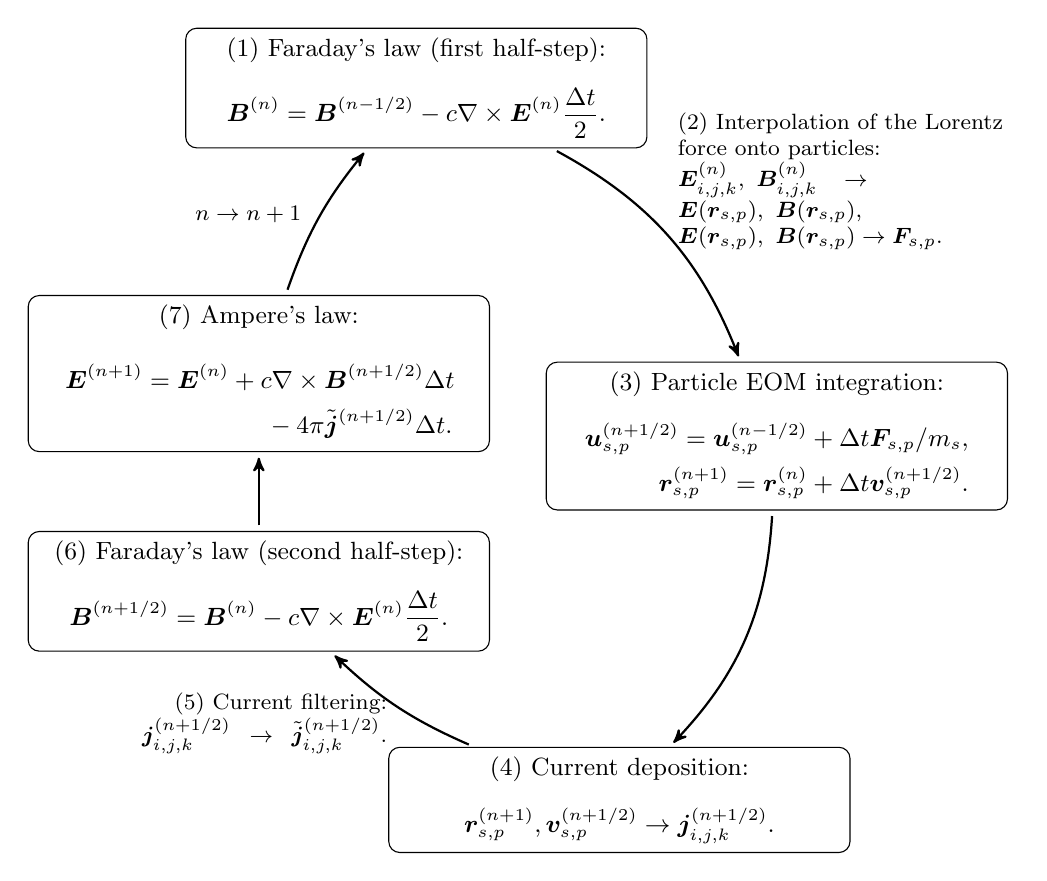
\begin{tikzpicture}[node distance=1cm, auto,]
  \node[box,xshift=2cm] (1) {
      (1) Faraday's law (first half-step): 
      \begin{equation*}
        \bm{B}^{(n)} = \bm{B}^{(n-1/2)} -c\nabla\times\bm{E}^{(n)}\frac{\Delta t}{2}.
      \end{equation*}
    };
  \node[box,below right=of 1,xshift=-2cm,yshift=-2cm] (3) {
      (3) Particle EOM integration: 
      \begin{equation*}
      \begin{aligned}
        \bm{u}_{s,p}^{(n+1/2)} = \bm{u}_{s,p}^{(n-1/2)} + \Delta t \bm{F}_{s,p}/m_s,\\
        \bm{r}_{s,p}^{(n+1)} = \bm{r}_{s,p}^{(n)} + \Delta t \bm{v}_{s,p}^{(n+1/2)}.
      \end{aligned}
      \end{equation*}
    };
  \node[box,below=of 3,yshift=-2cm,xshift=-2cm] (4) {
      (4) Current deposition: 
      \begin{equation*}
        \bm{r}_{s,p}^{(n+1)}, \bm{v}_{s,p}^{(n+1/2)}\rightarrow \bm{j}^{(n+1/2)}_{i,j,k}.
      \end{equation*}
    };
  \node[box,above left=of 4,yshift=0.5cm,xshift=2cm] (6) {
      (6) Faraday's law (second half-step): 
      \begin{equation*}
        \bm{B}^{(n+1/2)} = \bm{B}^{(n)} - c\nabla\times \bm{E}^{(n)}\frac{\Delta t}{2}.
      \end{equation*}
    };
  \node[box,above=of 6] (7) {
      (7) Ampere's law: 
      \begin{multline*}
        \bm{E}^{(n+1)} = \bm{E}^{(n)} + c\nabla\times \bm{B}^{(n+1/2)}\Delta t \\- 4\pi \tilde{\bm{j}}^{(n+1/2)}\Delta t.
      \end{multline*}
    };
  \draw[arrow] (1) to[bend left=20] 
    node [float,midway,align=left,yshift=-0.3cm,xshift=0cm] {
      (2) Interpolation of the Lorentz force onto particles: \\
      $\bm{E}_{i,j,k}^{(n)},~\bm{B}_{i,j,k}^{(n)}\rightarrow \bm{E}(\bm{r}_{s,p}),~\bm{B}(\bm{r}_{s,p}),$
      $\bm{E}(\bm{r}_{s,p}),~\bm{B}(\bm{r}_{s,p})\rightarrow \bm{F}_{s,p}.$
    } 
    (3);
  \draw[arrow] (3) to[bend left=20] (4);
  \draw[arrow] (4) to[bend left=10]
    node [float,midway,align=right,yshift=0.3cm,xshift=0cm] {
      (5) Current filtering: 
      $\bm{j}^{(n+1/2)}_{i,j,k}\rightarrow \tilde{\bm{j}}^{(n+1/2)}_{i,j,k}.$
    } 
    (6);
  \draw[arrow] (6) to (7);
  \draw[arrow] (7) to[bend left=10] 
    node [font=\footnotesize,midway,yshift=-0.2cm,align=right] {
      $n\to n+1$
    } 
    (1);
\end{tikzpicture}
  \caption{Key steps of the particle-in-cell plasma simulation algorithm.\label{fig:pic-steps}}
\end{figure}

There are numerous implementations of this algorithm \REF. In particular, \texttt{Tristan-MP} \REF has long been a reliable code widely used by the relativistic plasma astrophysics community. It is designed with the \texttt{Fortran 90} standards and parallelized using \texttt{MPI} libraries. \texttt{Tristan-MP v2} \REF~is the new incarnation of the original code with various added capabilities and optimizations. I will discuss some of the new capabilities, such as the radiation and quantum electrodynamic effects, in one of the following sections. Meanwhile, in the following section I describe another important advancement in the new code, aimed to help simulate plasmas in global astrophysical systems, where physically relevant scales are separated by many orders of magnitudes.

%\begin{figure}
  %\centering
  %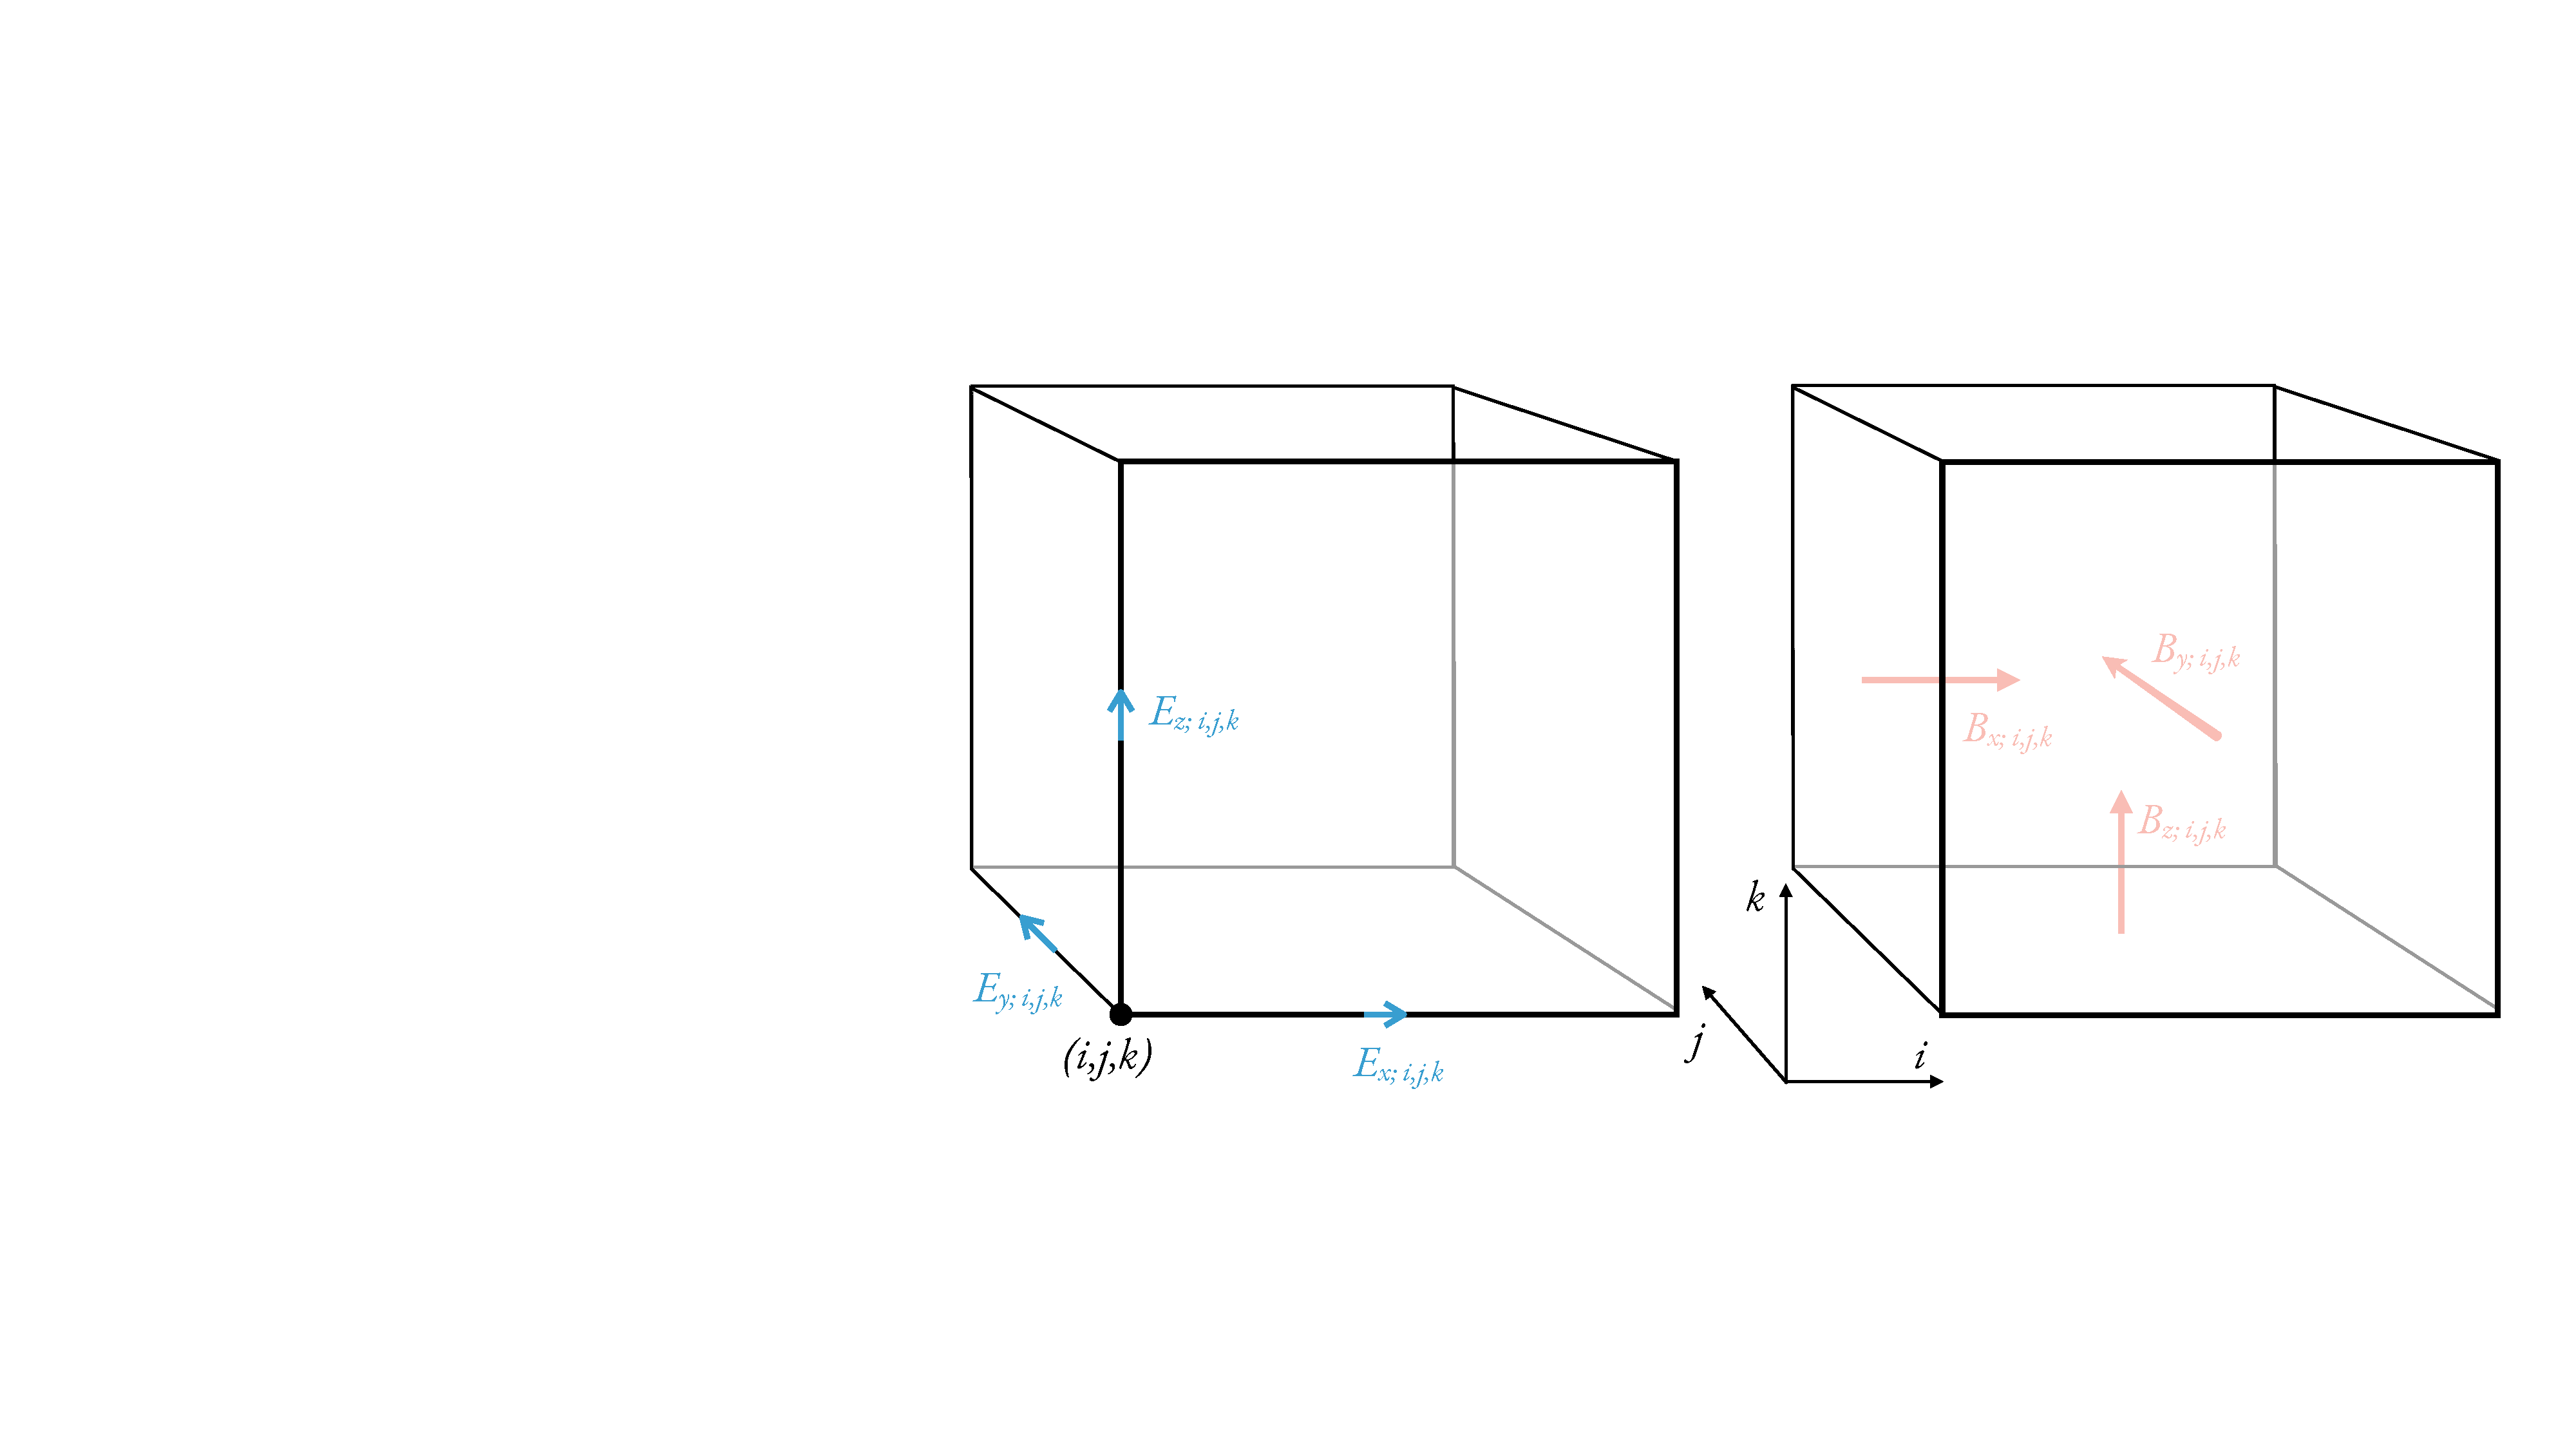
\includegraphics[trim=720 250 20 250,clip,width=0.7\textwidth]{figures/ch1-yee-mesh}
  %\caption[Yee mesh.]{Yee lattice configuration for the discretization of the electromagnetic field components. \label{fig:ch1-yee}}
%\end{figure}

\section{Highly magnetized (guiding center) approximation}

One of the main bottlenecks on the performance of the codes that employ PIC algorithms is the integration of particles' equations of motion (step 3 in figure~\ref{fig:pic-steps}); sometimes also called a \emph{particle push} substep. This integration is typically done using an explicit scheme with several substeps: 

\begin{align}
  \bm{r}^{(n+1/2)} &= \bm{r}^{(n)} + \frac{\bm{u}^{(n)}}{2\gamma^{(n)}}\Delta t,\\
  \frac{\bm{u}^{(n+1)}-\bm{u}^{(n)}}{\Delta t} &= \frac{1}{m_s} \bm{F}_{s,p}^{(n+1/2)},\label{eq:part-push2}\\
  \bm{r}^{(n+1)} &= \bm{r}^{(n+1/2)} + \frac{\bm{u}^{(n+1)}}{2\gamma^{(n+1)}}\Delta t.
\end{align}

\noindent Notice, that the Lorentz force, $\bm{F}_{s,p}$, in this scheme shall contain the particle's velocity \eqref{eq:lorentz-force}. In general, equation \eqref{eq:part-push2} is implicit with respect to the $\bm{u}^{(n+1)}$. However, typically, explicit approach is used for solving it. One of the most commonly used ones is the \emph{Boris algorithm} \REF, which is performed in three substeps:
\begin{equation}
  \begin{aligned}
    \textrm{half electric acceleration:  }&\bm{u}^- = \bm{u}^{(n)} + \frac{q_s}{m_s}\bm{E}(\bm{r}^{(n+1/2)})\frac{\Delta t}{2}, \\
    \textrm{magnetic rotation:  }& \bm{u}^+  = \bm{u}^- + (\bm{u}^-+\bm{u}^-\times \bm{t})\times\bm{s},\\
    \textrm{half electric acceleration:  }&\bm{u}^{(n+1)} = \bm{u}^+ + \frac{q_s}{m_s}\bm{E}(\bm{r}^{(n+1/2)})\frac{\Delta t}{2}.
  \end{aligned}
\end{equation}

\noindent Here $\bm{u}^\pm$ are intermediate variables, while 
\begin{equation}
  \bm{t} = \frac{q_s}{m_s}\frac{1}{\gamma^\pm }\bm{B}(\bm{r}^{(n+1/2)}) \frac{\Delta t}{2 c}, \textrm{ and } \bm{s} = \frac{2\bm{t}}{1 + |\bm{t}|^2}. 
\end{equation}
\noindent $\gamma^\pm$ are the Lorentz factors corresponding to intermediate velocities $\gamma^\pm = \sqrt{1 + (\bm{u}^{\pm})^2}$. Notice that they are equal, $\gamma^+ = \gamma^-$, i.e., the magnetic rotation substep does not modify particle's energy.\footnote{This result makes perfect physical sense as the magnetic field cannot impose work on charged particles.} There are numerous other integration schemes for the equations of motion; for a more detailed comprehensive overview and comparison see \REF. 

  %\newthought{There's something to be said} for having a good opening line. Morbi commodo, ipsum sed pharetra gravida, orci  $x = 1/\alpha$ magna rhoncus neque, id pulvinar odio lorem non turpis \cite{Eigen1971, Knuth1968}. Nullam sit amet enim. Suspendisse id velit vitae ligula volutpat condimentum. Aliquam erat volutpat. Sed quis velit. Nulla facilisi. Nulla libero. Vivamus pharetra posuere sapien. Nam consectetuer. Sed aliquam, nunc eget euismod ullamcorper, lectus nunc ullamcorper orci, fermentum bibendum enim nibh eget ipsum. Donec porttitor ligula eu dolor. Maecenas vitae nulla consequat libero cursus venenatis. Nam magna enim, accumsan eu, blandit sed, blandit a, eros.
  %$$\zeta = \frac{1039}{\pi}$$


  %% For an example of a full page figure, see Fig.~\ref{fig:myFullPageFigure}.

  %Lorem ipsum dolor sit amet, consectetuer adipiscing elit. Morbi commodo, ipsum sed pharetra gravida, orci magna rhoncus neque, id pulvinar odio lorem non turpis. Nullam sit amet enim. Suspendisse id velit vitae ligula volutpat condimentum. Aliquam erat volutpat. Sed quis velit. Nulla facilisi. Nulla libero. Vivamus pharetra posuere sapien. Nam consectetuer. Sed aliquam, nunc eget euismod ullamcorper, lectus nunc ullamcorper orci, fermentum bibendum enim nibh eget ipsum. Donec porttitor ligula eu dolor. Maecenas vitae nulla consequat libero cursus venenatis. Nam magna enim, accumsan eu, blandit sed, blandit a, eros.

  %Quisque facilisis erat a dui. Nam malesuada ornare dolor. Cras gravida, diam sit amet rhoncus ornare, erat elit consectetuer erat, id egestas pede nibh eget odio. Proin tincidunt, velit vel porta elementum, magna diam molestie sapien, non aliquet massa pede eu diam. Aliquam iaculis. Fusce et ipsum et nulla tristique facilisis. Donec eget sem sit amet ligula viverra gravida. Etiam vehicula urna vel turpis. Suspendisse sagittis ante a urna. Morbi a est quis orci consequat rutrum. Nullam egestas feugiat felis. Integer adipiscing semper ligula. Nunc molestie, nisl sit amet cursus convallis, sapien lectus pretium metus, vitae pretium enim wisi id lectus. Donec vestibulum. Etiam vel nibh. Nulla facilisi. Mauris pharetra. Donec augue. Fusce ultrices, neque id dignissim ultrices, tellus mauris dictum elit, vel lacinia enim metus eu nunc.

  %Pellentesque habitant morbi tristique senectus et netus et malesuada fames ac turpis egestas. Vestibulum tortor quam, feugiat vitae, ultricies eget, tempor sit amet, ante. Donec eu libero sit amet quam egestas semper. Aenean ultricies mi vitae est. Mauris placerat eleifend leo. Quisque sit amet est et sapien ullamcorper pharetra. Vestibulum erat wisi, condimentum sed, commodo vitae, ornare sit amet, wisi. Aenean fermentum, elit eget tincidunt condimentum, eros ipsum rutrum orci, sagittis tempus lacus enim ac dui. Donec non enim in turpis pulvinar facilisis. Ut felis.

  %Cras sed ante. Phasellus in massa. Curabitur dolor eros, gravida et, hendrerit ac, cursus non, massa. Aliquam lorem. In hac habitasse platea dictumst. Cras eu mauris. Quisque lacus. Donec ipsum. Nullam vitae sem at nunc pharetra ultricies. Vivamus elit eros, ullamcorper a, adipiscing sit amet, porttitor ut, nibh. Maecenas adipiscing mollis massa. Nunc ut dui eget nulla venenatis aliquet. Sed luctus posuere justo. Cras vehicula varius turpis. Vivamus eros metus, tristique sit amet, molestie dignissim, malesuada et, urna.

  %Cras dictum. Maecenas ut turpis. In vitae erat ac orci dignissim eleifend. Nunc quis justo. Sed vel ipsum in purus tincidunt pharetra. Sed pulvinar, felis id consectetuer malesuada, enim nisl mattis elit, a facilisis tortor nibh quis leo. Sed augue lacus, pretium vitae, molestie eget, rhoncus quis, elit. Donec in augue. Fusce orci wisi, ornare id, mollis vel, lacinia vel, massa.

  %Lorem ipsum dolor sit amet, consectetuer adipiscing elit. Morbi commodo, ipsum sed pharetra gravida, orci magna rhoncus neque, id pulvinar odio lorem non turpis. Nullam sit amet enim. Suspendisse id velit vitae ligula volutpat condimentum. Aliquam erat volutpat. Sed quis velit. Nulla facilisi. Nulla libero. Vivamus pharetra posuere sapien. Nam consectetuer. Sed aliquam, nunc eget euismod ullamcorper, lectus nunc ullamcorper orci, fermentum bibendum enim nibh eget ipsum. Donec porttitor ligula eu dolor. Maecenas vitae nulla consequat libero cursus venenatis. Nam magna enim, accumsan eu, blandit sed, blandit a, eros.

  %Quisque facilisis erat a dui. Nam malesuada ornare dolor. Cras gravida, diam sit amet rhoncus ornare, erat elit consectetuer erat, id egestas pede nibh eget odio. Proin tincidunt, velit vel porta elementum, magna diam molestie sapien, non aliquet massa pede eu diam. Aliquam iaculis. Fusce et ipsum et nulla tristique facilisis. Donec eget sem sit amet ligula viverra gravida. Etiam vehicula urna vel turpis. Suspendisse sagittis ante a urna. Morbi a est quis orci consequat rutrum. Nullam egestas feugiat felis. Integer adipiscing semper ligula. Nunc molestie, nisl sit amet cursus convallis, sapien lectus pretium metus, vitae pretium enim wisi id lectus. Donec vestibulum. Etiam vel nibh. Nulla facilisi. Mauris pharetra. Donec augue. Fusce ultrices, neque id dignissim ultrices, tellus mauris dictum elit, vel lacinia enim metus eu nunc.

  %\texttt{This is a line of code.}

  %Proin at eros non eros adipiscing mollis. Donec semper turpis sed diam. Sed consequat ligula nec tortor. Integer eget sem. Ut vitae enim eu est vehicula gravida. Morbi ipsum ipsum, porta nec, tempor id, auctor vitae, purus. Pellentesque neque. Nulla luctus erat vitae libero. Integer nec enim. Phasellus aliquam enim et tortor. Quisque aliquet, quam elementum condimentum feugiat, tellus odio consectetuer wisi, vel nonummy sem neque in elit. Curabitur eleifend wisi iaculis ipsum. Pellentesque habitant morbi tristique senectus et netus et malesuada fames ac turpis egestas. In non velit non ligula laoreet ultrices. Praesent ultricies facilisis nisl. Vivamus luctus elit sit amet mi. Phasellus pellentesque, erat eget elementum volutpat, dolor nisl porta neque, vitae sodales ipsum nibh in ligula. Maecenas mattis pulvinar diam. Curabitur sed leo.

  %Nulla facilisi. In vel sem. Morbi id urna in diam dignissim feugiat. Proin molestie tortor eu velit. Aliquam erat volutpat. Nullam ultrices, diam tempus vulputate egestas, eros pede varius leo, sed imperdiet lectus est ornare odio. Lorem ipsum dolor sit amet, consectetuer adipiscing elit. Proin consectetuer velit in dui. Phasellus wisi purus, interdum vitae, rutrum accumsan, viverra in, velit. Sed enim risus, congue non, tristique in, commodo eu, metus. Aenean tortor mi, imperdiet id, gravida eu, posuere eu, felis. Mauris sollicitudin, turpis in hendrerit sodales, lectus ipsum pellentesque ligula, sit amet scelerisque urna nibh ut arcu. Aliquam in lacus. Vestibulum ante ipsum primis in faucibus orci luctus et ultrices posuere cubilia Curae; Nulla placerat aliquam wisi. Mauris viverra odio. Quisque fermentum pulvinar odio. Proin posuere est vitae ligula. Etiam euismod. Cras a eros.

  %Nunc auctor bibendum eros. Maecenas porta accumsan mauris. Etiam enim enim, elementum sed, bibendum quis, rhoncus non, metus. Fusce neque dolor, adipiscing sed, consectetuer et, lacinia sit amet, quam. Suspendisse wisi quam, consectetuer in, blandit sed, suscipit eu, eros. Etiam ligula enim, tempor ut, blandit nec, mollis eu, lectus. Nam cursus. Vivamus iaculis. Aenean risus purus, pharetra in, blandit quis, gravida a, turpis. Donec nisl. Aenean eget mi. Fusce mattis est id diam. Phasellus faucibus interdum sapien. Duis quis nunc. Sed enim.

  %Pellentesque vel dui sed orci faucibus iaculis. Suspendisse dictum magna id purus tincidunt rutrum. Nulla congue. Vivamus sit amet lorem posuere dui vulputate ornare. Phasellus mattis sollicitudin ligula. Duis dignissim felis et urna. Integer adipiscing congue metus. Nam pede. Etiam non wisi. Sed accumsan dolor ac augue. Pellentesque eget lectus. Aliquam nec dolor nec tellus ornare venenatis. Nullam blandit placerat sem. Curabitur quis ipsum. Mauris nisl tellus, aliquet eu, suscipit eu, ullamcorper quis, magna. Mauris elementum, pede at sodales vestibulum, nulla tortor congue massa, quis pellentesque odio dui id est. Cras faucibus augue.

  %Suspendisse vestibulum dignissim quam. Integer vel augue. Phasellus nulla purus, interdum ac, venenatis non, varius rutrum, leo. Pellentesque habitant morbi tristique senectus et netus et malesuada fames ac turpis egestas. Duis a eros. Class aptent taciti sociosqu ad litora torquent per conubia nostra, per inceptos hymenaeos. Fusce magna mi, porttitor quis, convallis eget, sodales ac, urna. Phasellus luctus venenatis magna. Vivamus eget lacus. Nunc tincidunt convallis tortor. Duis eros mi, dictum vel, fringilla sit amet, fermentum id, sem. Phasellus nunc enim, faucibus ut, laoreet in, consequat id, metus. Vivamus dignissim. Cras lobortis tempor velit. Phasellus nec diam ac nisl lacinia tristique. Nullam nec metus id mi dictum dignissim. Nullam quis wisi non sem lobortis condimentum. Phasellus pulvinar, nulla non aliquam eleifend, tortor wisi scelerisque felis, in sollicitudin arcu ante lacinia leo.

  %Pellentesque habitant morbi tristique senectus et netus et malesuada fames ac turpis egestas. Vestibulum tortor quam, feugiat vitae, ultricies eget, tempor sit amet, ante. Donec eu libero sit amet quam egestas semper. Aenean ultricies mi vitae est. Mauris placerat eleifend leo. Quisque sit amet est et sapien ullamcorper pharetra. Vestibulum erat wisi, condimentum sed, commodo vitae, ornare sit amet, wisi. Aenean fermentum, elit eget tincidunt condimentum, eros ipsum rutrum orci, sagittis tempus lacus enim ac dui. Donec non enim in turpis pulvinar facilisis. Ut felis.

  %Cras sed ante. Phasellus in massa. Curabitur dolor eros, gravida et, hendrerit ac, cursus non, massa. Aliquam lorem. In hac habitasse platea dictumst. Cras eu mauris. Quisque lacus. Donec ipsum. Nullam vitae sem at nunc pharetra ultricies. Vivamus elit eros, ullamcorper a, adipiscing sit amet, porttitor ut, nibh. Maecenas adipiscing mollis massa. Nunc ut dui eget nulla venenatis aliquet. Sed luctus posuere justo. Cras vehicula varius turpis. Vivamus eros metus, tristique sit amet, molestie dignissim, malesuada et, urna.

  %Cras dictum. Maecenas ut turpis. In vitae erat ac orci dignissim eleifend. Nunc quis justo. Sed vel ipsum in purus tincidunt pharetra. Sed pulvinar, felis id consectetuer malesuada, enim nisl mattis elit, a facilisis tortor nibh quis leo. Sed augue lacus, pretium vitae, molestie eget, rhoncus quis, elit. Donec in augue. Fusce orci wisi, ornare id, mollis vel, lacinia vel, massa.

  %Lorem ipsum dolor sit amet, consectetuer adipiscing elit. Morbi commodo, ipsum sed pharetra gravida, orci magna rhoncus neque, id pulvinar odio lorem non turpis. Nullam sit amet enim. Suspendisse id velit vitae ligula volutpat condimentum. Aliquam erat volutpat. Sed quis velit. Nulla facilisi. Nulla libero. Vivamus pharetra posuere sapien. Nam consectetuer. Sed aliquam, nunc eget euismod ullamcorper, lectus nunc ullamcorper orci, fermentum bibendum enim nibh eget ipsum. Donec porttitor ligula eu dolor. Maecenas vitae nulla consequat libero cursus venenatis. Nam magna enim, accumsan eu, blandit sed, blandit a, eros.


  %\begin{figure}
  %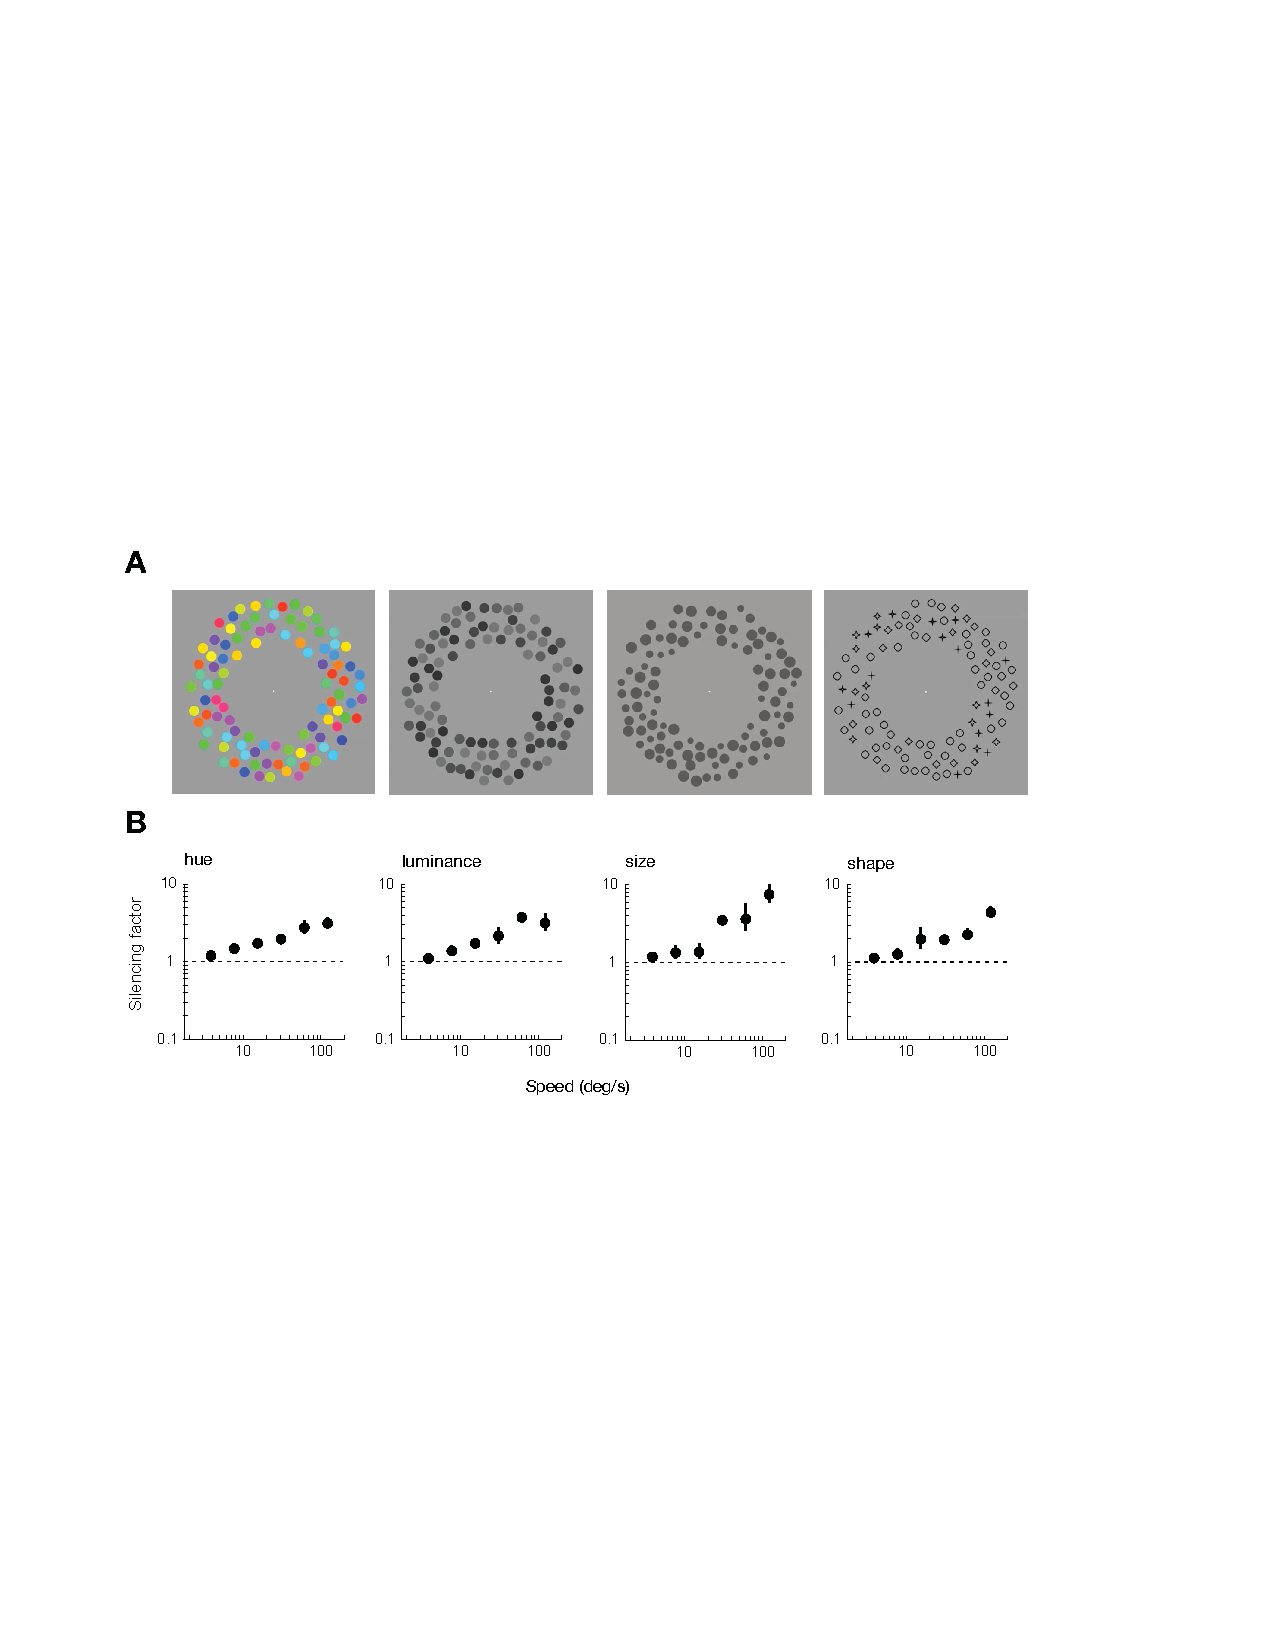
\includegraphics[width=\textwidth]{figures/fig1}
  %\caption[Short figure name.]{This is a figure that floats inline and here is its caption.
  %\label{fig:myInlineFigure}}
  %\end{figure}


  %Quisque facilisis erat a dui. Nam malesuada ornare dolor. Cras gravida, diam sit amet rhoncus ornare, erat elit consectetuer erat, id egestas pede nibh eget odio. Proin tincidunt, velit vel porta elementum, magna diam molestie sapien, non aliquet massa pede eu diam. Aliquam iaculis. Fusce et ipsum et nulla tristique facilisis. Donec eget sem sit amet ligula viverra gravida. Etiam vehicula urna vel turpis. Suspendisse sagittis ante a urna. Morbi a est quis orci consequat rutrum. Nullam egestas feugiat felis. Integer adipiscing semper ligula. Nunc molestie, nisl sit amet cursus convallis, sapien lectus pretium metus, vitae pretium enim wisi id lectus. Donec vestibulum. Etiam vel nibh. Nulla facilisi. Mauris pharetra. Donec augue. Fusce ultrices, neque id dignissim ultrices, tellus mauris dictum elit, vel lacinia enim metus eu nunc.

  %Proin at eros non eros adipiscing mollis. Donec semper turpis sed diam. Sed consequat ligula nec tortor. Integer eget sem. Ut vitae enim eu est vehicula gravida. Morbi ipsum ipsum, porta nec, tempor id, auctor vitae, purus. Pellentesque neque. Nulla luctus erat vitae libero. Integer nec enim. Phasellus aliquam enim et tortor. Quisque aliquet, quam elementum condimentum feugiat, tellus odio consectetuer wisi, vel nonummy sem neque in elit. Curabitur eleifend wisi iaculis ipsum. Pellentesque habitant morbi tristique senectus et netus et malesuada fames ac turpis egestas. In non velit non ligula laoreet ultrices. Praesent ultricies facilisis nisl. Vivamus luctus elit sit amet mi. Phasellus pellentesque, erat eget elementum volutpat, dolor nisl porta neque, vitae sodales ipsum nibh in ligula. Maecenas mattis pulvinar diam. Curabitur sed leo.

  %Nulla facilisi. In vel sem. Morbi id urna in diam dignissim feugiat. Proin molestie tortor eu velit. Aliquam erat volutpat. Nullam ultrices, diam tempus vulputate egestas, eros pede varius leo, sed imperdiet lectus est ornare odio. Lorem ipsum dolor sit amet, consectetuer adipiscing elit. Proin consectetuer velit in dui. Phasellus wisi purus, interdum vitae, rutrum accumsan, viverra in, velit. Sed enim risus, congue non, tristique in, commodo eu, metus. Aenean tortor mi, imperdiet id, gravida eu, posuere eu, felis. Mauris sollicitudin, turpis in hendrerit sodales, lectus ipsum pellentesque ligula, sit amet scelerisque urna nibh ut arcu. Aliquam in lacus. Vestibulum ante ipsum primis in faucibus orci luctus et ultrices posuere cubilia Curae; Nulla placerat aliquam wisi. Mauris viverra odio. Quisque fermentum pulvinar odio. Proin posuere est vitae ligula. Etiam euismod. Cras a eros.

  %Nunc auctor bibendum eros. Maecenas porta accumsan mauris. Etiam enim enim, elementum sed, bibendum quis, rhoncus non, metus. Fusce neque dolor, adipiscing sed, consectetuer et, lacinia sit amet, quam. Suspendisse wisi quam, consectetuer in, blandit sed, suscipit eu, eros. Etiam ligula enim, tempor ut, blandit nec, mollis eu, lectus. Nam cursus. Vivamus iaculis. Aenean risus purus, pharetra in, blandit quis, gravida a, turpis. Donec nisl. Aenean eget mi. Fusce mattis est id diam. Phasellus faucibus interdum sapien. Duis quis nunc. Sed enim.

  %Pellentesque vel dui sed orci faucibus iaculis. Suspendisse dictum magna id purus tincidunt rutrum. Nulla congue. Vivamus sit amet lorem posuere dui vulputate ornare. Phasellus mattis sollicitudin ligula. Duis dignissim felis et urna. Integer adipiscing congue metus. Nam pede. Etiam non wisi. Sed accumsan dolor ac augue. Pellentesque eget lectus. Aliquam nec dolor nec tellus ornare venenatis. Nullam blandit placerat sem. Curabitur quis ipsum. Mauris nisl tellus, aliquet eu, suscipit eu, ullamcorper quis, magna. Mauris elementum, pede at sodales vestibulum, nulla tortor congue massa, quis pellentesque odio dui id est. Cras faucibus augue.

  %%% Requires fltpage2 package
  %%%
  %% \begin{FPfigure}
  %% 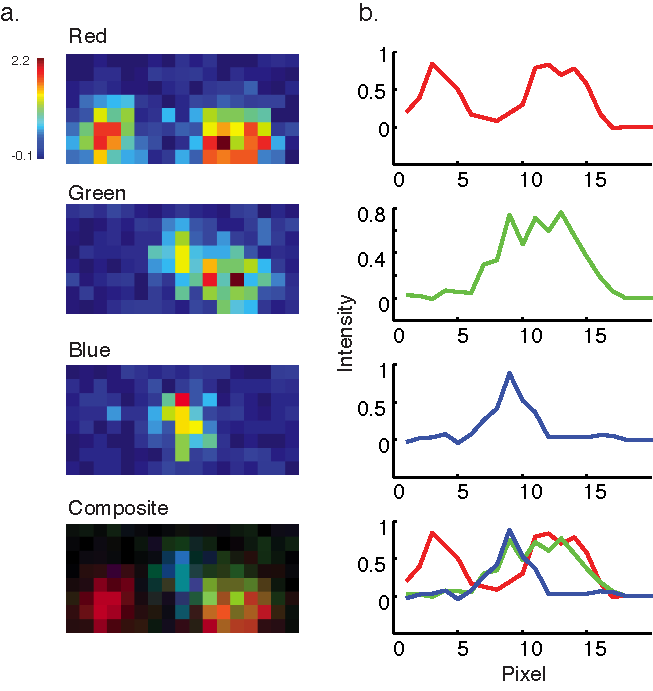
\includegraphics[width=\textwidth]{figures/fullpage}
  %% \caption[Short figure name.]{This is a full page figure using the FPfigure command. It takes up the whole page and the caption appears on the preceding page. Its useful for large figures. Harvard's rules about full page figures are tricky, but you don't have to worry about it because we took care of it for you. For example, the full figure is supposed to have a title in the same style as the caption but without the actual caption. The caption is supposed to appear alone on the preceding page with no other text. You do't have to worry about any of that. We have modified the fltpage package to make it work. This is a lengthy caption and it clearly would not fit on the same page as the figure. Note that you should only use the FPfigure command in instances where the figure really is too large. If the figure is small enough to fit by the caption than it does not produce the desired effect. Good luck with your thesis. I have to keep writing this to make the caption really long. LaTex is a lot of fun. You will enjoy working with it. Good luck on your post doctoral life! I am looking forward to mine. \label{fig:myFullPageFigure}}
  %% \end{FPfigure}
  %% \afterpage{\clearpage}

  %Suspendisse vestibulum dignissim quam. Integer vel augue. Phasellus nulla purus, interdum ac, venenatis non, varius rutrum, leo. Pellentesque habitant morbi tristique senectus et netus et malesuada fames ac turpis egestas. Duis a eros. Class aptent taciti sociosqu ad litora torquent per conubia nostra, per inceptos hymenaeos. Fusce magna mi, porttitor quis, convallis eget, sodales ac, urna. Phasellus luctus venenatis magna. Vivamus eget lacus. Nunc tincidunt convallis tortor. Duis eros mi, dictum vel, fringilla sit amet, fermentum id, sem. Phasellus nunc enim, faucibus ut, laoreet in, consequat id, metus. Vivamus dignissim. Cras lobortis tempor velit. Phasellus nec diam ac nisl lacinia tristique. Nullam nec metus id mi dictum dignissim. Nullam quis wisi non sem lobortis condimentum. Phasellus pulvinar, nulla non aliquam eleifend, tortor wisi scelerisque felis, in sollicitudin arcu ante lacinia leo.

  %Pellentesque habitant morbi tristique senectus et netus et malesuada fames ac turpis egestas. Vestibulum tortor quam, feugiat vitae, ultricies eget, tempor sit amet, ante. Donec eu libero sit amet quam egestas semper. Aenean ultricies mi vitae est. Mauris placerat eleifend leo. Quisque sit amet est et sapien ullamcorper pharetra. Vestibulum erat wisi, condimentum sed, commodo vitae, ornare sit amet, wisi. Aenean fermentum, elit eget tincidunt condimentum, eros ipsum rutrum orci, sagittis tempus lacus enim ac dui. Donec non enim in turpis pulvinar facilisis. Ut felis.

  %Cras sed ante. Phasellus in massa. Curabitur dolor eros, gravida et, hendrerit ac, cursus non, massa. Aliquam lorem. In hac habitasse platea dictumst. Cras eu mauris. Quisque lacus. Donec ipsum. Nullam vitae sem at nunc pharetra ultricies. Vivamus elit eros, ullamcorper a, adipiscing sit amet, porttitor ut, nibh. Maecenas adipiscing mollis massa. Nunc ut dui eget nulla venenatis aliquet. Sed luctus posuere justo. Cras vehicula varius turpis. Vivamus eros metus, tristique sit amet, molestie dignissim, malesuada et, urna.

  %Proin at eros non eros adipiscing mollis. Donec semper turpis sed diam. Sed consequat ligula nec tortor. Integer eget sem. Ut vitae enim eu est vehicula gravida. Morbi ipsum ipsum, porta nec, tempor id, auctor vitae, purus. Pellentesque neque. Nulla luctus erat vitae libero. Integer nec enim. Phasellus aliquam enim et tortor. Quisque aliquet, quam elementum condimentum feugiat, tellus odio consectetuer wisi, vel nonummy sem neque in elit. Curabitur eleifend wisi iaculis ipsum. Pellentesque habitant morbi tristique senectus et netus et malesuada fames ac turpis egestas. In non velit non ligula laoreet ultrices. Praesent ultricies facilisis nisl. Vivamus luctus elit sit amet mi. Phasellus pellentesque, erat eget elementum volutpat, dolor nisl porta neque, vitae sodales ipsum nibh in ligula. Maecenas mattis pulvinar diam. Curabitur sed leo.

  %Nulla facilisi. In vel sem. Morbi id urna in diam dignissim feugiat. Proin molestie tortor eu velit. Aliquam erat volutpat. Nullam ultrices, diam tempus vulputate egestas, eros pede varius leo, sed imperdiet lectus est ornare odio. Lorem ipsum dolor sit amet, consectetuer adipiscing elit. Proin consectetuer velit in dui. Phasellus wisi purus, interdum vitae, rutrum accumsan, viverra in, velit. Sed enim risus, congue non, tristique in, commodo eu, metus. Aenean tortor mi, imperdiet id, gravida eu, posuere eu, felis. Mauris sollicitudin, turpis in hendrerit sodales, lectus ipsum pellentesque ligula, sit amet scelerisque urna nibh ut arcu. Aliquam in lacus. Vestibulum ante ipsum primis in faucibus orci luctus et ultrices posuere cubilia Curae; Nulla placerat aliquam wisi. Mauris viverra odio. Quisque fermentum pulvinar odio. Proin posuere est vitae ligula. Etiam euismod. Cras a eros.

  %Nunc auctor bibendum eros. Maecenas porta accumsan mauris. Etiam enim enim, elementum sed, bibendum quis, rhoncus non, metus. Fusce neque dolor, adipiscing sed, consectetuer et, lacinia sit amet, quam. Suspendisse wisi quam, consectetuer in, blandit sed, suscipit eu, eros. Etiam ligula enim, tempor ut, blandit nec, mollis eu, lectus. Nam cursus. Vivamus iaculis. Aenean risus purus, pharetra in, blandit quis, gravida a, turpis. Donec nisl. Aenean eget mi. Fusce mattis est id diam. Phasellus faucibus interdum sapien. Duis quis nunc. Sed enim.

  %Pellentesque vel dui sed orci faucibus iaculis. Suspendisse dictum magna id purus tincidunt rutrum. Nulla congue. Vivamus sit amet lorem posuere dui vulputate ornare. Phasellus mattis sollicitudin ligula. Duis dignissim felis et urna. Integer adipiscing congue metus. Nam pede. Etiam non wisi. Sed accumsan dolor ac augue. Pellentesque eget lectus. Aliquam nec dolor nec tellus ornare venenatis. Nullam blandit placerat sem. Curabitur quis ipsum. Mauris nisl tellus, aliquet eu, suscipit eu, ullamcorper quis, magna. Mauris elementum, pede at sodales vestibulum, nulla tortor congue massa, quis pellentesque odio dui id est. Cras faucibus augue.

  %Suspendisse vestibulum dignissim quam. Integer vel augue. Phasellus nulla purus, interdum ac, venenatis non, varius rutrum, leo. Pellentesque habitant morbi tristique senectus et netus et malesuada fames ac turpis egestas. Duis a eros. Class aptent taciti sociosqu ad litora torquent per conubia nostra, per inceptos hymenaeos. Fusce magna mi, porttitor quis, convallis eget, sodales ac, urna. Phasellus luctus venenatis magna. Vivamus eget lacus. Nunc tincidunt convallis tortor. Duis eros mi, dictum vel, fringilla sit amet, fermentum id, sem. Phasellus nunc enim, faucibus ut, laoreet in, consequat id, metus. Vivamus dignissim. Cras lobortis tempor velit. Phasellus nec diam ac nisl lacinia tristique. Nullam nec metus id mi dictum dignissim. Nullam quis wisi non sem lobortis condimentum. Phasellus pulvinar, nulla non aliquam eleifend, tortor wisi scelerisque felis, in sollicitudin arcu ante lacinia leo.

  %Pellentesque habitant morbi tristique senectus et netus et malesuada fames ac turpis egestas. Vestibulum tortor quam, feugiat vitae, ultricies eget, tempor sit amet, ante. Donec eu libero sit amet quam egestas semper. Aenean ultricies mi vitae est. Mauris placerat eleifend leo. Quisque sit amet est et sapien ullamcorper pharetra. Vestibulum erat wisi, condimentum sed, commodo vitae, ornare sit amet, wisi. Aenean fermentum, elit eget tincidunt condimentum, eros ipsum rutrum orci, sagittis tempus lacus enim ac dui. Donec non enim in turpis pulvinar facilisis. Ut felis.

  %Cras sed ante. Phasellus in massa. Curabitur dolor eros, gravida et, hendrerit ac, cursus non, massa. Aliquam lorem. In hac habitasse platea dictumst. Cras eu mauris. Quisque lacus. Donec ipsum. Nullam vitae sem at nunc pharetra ultricies. Vivamus elit eros, ullamcorper a, adipiscing sit amet, porttitor ut, nibh. Maecenas adipiscing mollis massa. Nunc ut dui eget nulla venenatis aliquet. Sed luctus posuere justo. Cras vehicula varius turpis. Vivamus eros metus, tristique sit amet, molestie dignissim, malesuada et, urna.

  %Cras dictum. Maecenas ut turpis. In vitae erat ac orci dignissim eleifend. Nunc quis justo. Sed vel ipsum in purus tincidunt pharetra. Sed pulvinar, felis id consectetuer malesuada, enim nisl mattis elit, a facilisis tortor nibh quis leo. Sed augue lacus, pretium vitae, molestie eget, rhoncus quis, elit. Donec in augue. Fusce orci wisi, ornare id, mollis vel, lacinia vel, massa.

  %Lorem ipsum dolor sit amet, consectetuer adipiscing elit. Morbi commodo, ipsum sed pharetra gravida, orci magna rhoncus neque, id pulvinar odio lorem non turpis. Nullam sit amet enim. Suspendisse id velit vitae ligula volutpat condimentum. Aliquam erat volutpat. Sed quis velit. Nulla facilisi. Nulla libero. Vivamus pharetra posuere sapien. Nam consectetuer. Sed aliquam, nunc eget euismod ullamcorper, lectus nunc ullamcorper orci, fermentum bibendum enim nibh eget ipsum. Donec porttitor ligula eu dolor. Maecenas vitae nulla consequat libero cursus venenatis. Nam magna enim, accumsan eu, blandit sed, blandit a, eros.

  %Quisque facilisis erat a dui. Nam malesuada ornare dolor. Cras gravida, diam sit amet rhoncus ornare, erat elit consectetuer erat, id egestas pede nibh eget odio. Proin tincidunt, velit vel porta elementum, magna diam molestie sapien, non aliquet massa pede eu diam. Aliquam iaculis. Fusce et ipsum et nulla tristique facilisis. Donec eget sem sit amet ligula viverra gravida. Etiam vehicula urna vel turpis. Suspendisse sagittis ante a urna. Morbi a est quis orci consequat rutrum. Nullam egestas feugiat felis. Integer adipiscing semper ligula. Nunc molestie, nisl sit amet cursus convallis, sapien lectus pretium metus, vitae pretium enim wisi id lectus. Donec vestibulum. Etiam vel nibh. Nulla facilisi. Mauris pharetra. Donec augue. Fusce ultrices, neque id dignissim ultrices, tellus mauris dictum elit, vel lacinia enim metus eu nunc.

  %Proin at eros non eros adipiscing mollis. Donec semper turpis sed diam. Sed consequat ligula nec tortor. Integer eget sem. Ut vitae enim eu est vehicula gravida. Morbi ipsum ipsum, porta nec, tempor id, auctor vitae, purus. Pellentesque neque. Nulla luctus erat vitae libero. Integer nec enim. Phasellus aliquam enim et tortor. Quisque aliquet, quam elementum condimentum feugiat, tellus odio consectetuer wisi, vel nonummy sem neque in elit. Curabitur eleifend wisi iaculis ipsum. Pellentesque habitant morbi tristique senectus et netus et malesuada fames ac turpis egestas. In non velit non ligula laoreet ultrices. Praesent ultricies facilisis nisl. Vivamus luctus elit sit amet mi. Phasellus pellentesque, erat eget elementum volutpat, dolor nisl porta neque, vitae sodales ipsum nibh in ligula. Maecenas mattis pulvinar diam. Curabitur sed leo.

  %Nulla facilisi. In vel sem. Morbi id urna in diam dignissim feugiat. Proin molestie tortor eu velit. Aliquam erat volutpat. Nullam ultrices, diam tempus vulputate egestas, eros pede varius leo, sed imperdiet lectus est ornare odio. Lorem ipsum dolor sit amet, consectetuer adipiscing elit. Proin consectetuer velit in dui. Phasellus wisi purus, interdum vitae, rutrum accumsan, viverra in, velit. Sed enim risus, congue non, tristique in, commodo eu, metus. Aenean tortor mi, imperdiet id, gravida eu, posuere eu, felis. Mauris sollicitudin, turpis in hendrerit sodales, lectus ipsum pellentesque ligula, sit amet scelerisque urna nibh ut arcu. Aliquam in lacus. Vestibulum ante ipsum primis in faucibus orci luctus et ultrices posuere cubilia Curae; Nulla placerat aliquam wisi. Mauris viverra odio. Quisque fermentum pulvinar odio. Proin posuere est vitae ligula. Etiam euismod. Cras a eros.

  %Nunc auctor bibendum eros. Maecenas porta accumsan mauris. Etiam enim enim, elementum sed, bibendum quis, rhoncus non, metus. Fusce neque dolor, adipiscing sed, consectetuer et, lacinia sit amet, quam. Suspendisse wisi quam, consectetuer in, blandit sed, suscipit eu, eros. Etiam ligula enim, tempor ut, blandit nec, mollis eu, lectus. Nam cursus. Vivamus iaculis. Aenean risus purus, pharetra in, blandit quis, gravida a, turpis. Donec nisl. Aenean eget mi. Fusce mattis est id diam. Phasellus faucibus interdum sapien. Duis quis nunc. Sed enim.

  %Pellentesque vel dui sed orci faucibus iaculis. Suspendisse dictum magna id purus tincidunt rutrum. Nulla congue. Vivamus sit amet lorem posuere dui vulputate ornare. Phasellus mattis sollicitudin ligula. Duis dignissim felis et urna. Integer adipiscing congue metus. Nam pede. Etiam non wisi. Sed accumsan dolor ac augue. Pellentesque eget lectus. Aliquam nec dolor nec tellus ornare venenatis. Nullam blandit placerat sem. Curabitur quis ipsum. Mauris nisl tellus, aliquet eu, suscipit eu, ullamcorper quis, magna. Mauris elementum, pede at sodales vestibulum, nulla tortor congue massa, quis pellentesque odio dui id est. Cras faucibus augue.

  %Suspendisse vestibulum dignissim quam. Integer vel augue. Phasellus nulla purus, interdum ac, venenatis non, varius rutrum, leo. Pellentesque habitant morbi tristique senectus et netus et malesuada fames ac turpis egestas. Duis a eros. Class aptent taciti sociosqu ad litora torquent per conubia nostra, per inceptos hymenaeos. Fusce magna mi, porttitor quis, convallis eget, sodales ac, urna. Phasellus luctus venenatis magna. Vivamus eget lacus. Nunc tincidunt convallis tortor. Duis eros mi, dictum vel, fringilla sit amet, fermentum id, sem. Phasellus nunc enim, faucibus ut, laoreet in, consequat id, metus. Vivamus dignissim. Cras lobortis tempor velit. Phasellus nec diam ac nisl lacinia tristique. Nullam nec metus id mi dictum dignissim. Nullam quis wisi non sem lobortis condimentum. Phasellus pulvinar, nulla non aliquam eleifend, tortor wisi scelerisque felis, in sollicitudin arcu ante lacinia leo.

  %Pellentesque habitant morbi tristique senectus et netus et malesuada fames ac turpis egestas. Vestibulum tortor quam, feugiat vitae, ultricies eget, tempor sit amet, ante. Donec eu libero sit amet quam egestas semper. Aenean ultricies mi vitae est. Mauris placerat eleifend leo. Quisque sit amet est et sapien ullamcorper pharetra. Vestibulum erat wisi, condimentum sed, commodo vitae, ornare sit amet, wisi. Aenean fermentum, elit eget tincidunt condimentum, eros ipsum rutrum orci, sagittis tempus lacus enim ac dui. Donec non enim in turpis pulvinar facilisis. Ut felis.

  %Cras sed ante. Phasellus in massa. Curabitur dolor eros, gravida et, hendrerit ac, cursus non, massa. Aliquam lorem. In hac habitasse platea dictumst. Cras eu mauris. Quisque lacus. Donec ipsum. Nullam vitae sem at nunc pharetra ultricies. Vivamus elit eros, ullamcorper a, adipiscing sit amet, porttitor ut, nibh. Maecenas adipiscing mollis massa. Nunc ut dui eget nulla venenatis aliquet. Sed luctus posuere justo. Cras vehicula varius turpis. Vivamus eros metus, tristique sit amet, molestie dignissim, malesuada et, urna.

  %Cras dictum. Maecenas ut turpis. In vitae erat ac orci dignissim eleifend. Nunc quis justo. Sed vel ipsum in purus tincidunt pharetra. Sed pulvinar, felis id consectetuer malesuada, enim nisl mattis elit, a facilisis tortor nibh quis leo. Sed augue lacus, pretium vitae, molestie eget, rhoncus quis, elit. Donec in augue. Fusce orci wisi, ornare id, mollis vel, lacinia vel, massa.

  %Lorem ipsum dolor sit amet, consectetuer adipiscing elit. Morbi commodo, ipsum sed pharetra gravida, orci magna rhoncus neque, id pulvinar odio lorem non turpis. Nullam sit amet enim. Suspendisse id velit vitae ligula volutpat condimentum. Aliquam erat volutpat. Sed quis velit. Nulla facilisi. Nulla libero. Vivamus pharetra posuere sapien. Nam consectetuer. Sed aliquam, nunc eget euismod ullamcorper, lectus nunc ullamcorper orci, fermentum bibendum enim nibh eget ipsum. Donec porttitor ligula eu dolor. Maecenas vitae nulla consequat libero cursus venenatis. Nam magna enim, accumsan eu, blandit sed, blandit a, eros.

  %Quisque facilisis erat a dui. Nam malesuada ornare dolor. Cras gravida, diam sit amet rhoncus ornare, erat elit consectetuer erat, id egestas pede nibh eget odio. Proin tincidunt, velit vel porta elementum, magna diam molestie sapien, non aliquet massa pede eu diam. Aliquam iaculis. Fusce et ipsum et nulla tristique facilisis. Donec eget sem sit amet ligula viverra gravida. Etiam vehicula urna vel turpis. Suspendisse sagittis ante a urna. Morbi a est quis orci consequat rutrum. Nullam egestas feugiat felis. Integer adipiscing semper ligula. Nunc molestie, nisl sit amet cursus convallis, sapien lectus pretium metus, vitae pretium enim wisi id lectus. Donec vestibulum. Etiam vel nibh. Nulla facilisi. Mauris pharetra. Donec augue. Fusce ultrices, neque id dignissim ultrices, tellus mauris dictum elit, vel lacinia enim metus eu nunc.

  %Proin at eros non eros adipiscing mollis. Donec semper turpis sed diam. Sed consequat ligula nec tortor. Integer eget sem. Ut vitae enim eu est vehicula gravida. Morbi ipsum ipsum, porta nec, tempor id, auctor vitae, purus. Pellentesque neque. Nulla luctus erat vitae libero. Integer nec enim. Phasellus aliquam enim et tortor. Quisque aliquet, quam elementum condimentum feugiat, tellus odio consectetuer wisi, vel nonummy sem neque in elit. Curabitur eleifend wisi iaculis ipsum. Pellentesque habitant morbi tristique senectus et netus et malesuada fames ac turpis egestas. In non velit non ligula laoreet ultrices. Praesent ultricies facilisis nisl. Vivamus luctus elit sit amet mi. Phasellus pellentesque, erat eget elementum volutpat, dolor nisl porta neque, vitae sodales ipsum nibh in ligula. Maecenas mattis pulvinar diam. Curabitur sed leo.

  %Nulla facilisi. In vel sem. Morbi id urna in diam dignissim feugiat. Proin molestie tortor eu velit. Aliquam erat volutpat. Nullam ultrices, diam tempus vulputate egestas, eros pede varius leo, sed imperdiet lectus est ornare odio. Lorem ipsum dolor sit amet, consectetuer adipiscing elit. Proin consectetuer velit in dui. Phasellus wisi purus, interdum vitae, rutrum accumsan, viverra in, velit. Sed enim risus, congue non, tristique in, commodo eu, metus. Aenean tortor mi, imperdiet id, gravida eu, posuere eu, felis. Mauris sollicitudin, turpis in hendrerit sodales, lectus ipsum pellentesque ligula, sit amet scelerisque urna nibh ut arcu. Aliquam in lacus. Vestibulum ante ipsum primis in faucibus orci luctus et ultrices posuere cubilia Curae; Nulla placerat aliquam wisi. Mauris viverra odio. Quisque fermentum pulvinar odio. Proin posuere est vitae ligula. Etiam euismod. Cras a eros.

  %Nunc auctor bibendum eros. Maecenas porta accumsan mauris. Etiam enim enim, elementum sed, bibendum quis, rhoncus non, metus. Fusce neque dolor, adipiscing sed, consectetuer et, lacinia sit amet, quam. Suspendisse wisi quam, consectetuer in, blandit sed, suscipit eu, eros. Etiam ligula enim, tempor ut, blandit nec, mollis eu, lectus. Nam cursus. Vivamus iaculis. Aenean risus purus, pharetra in, blandit quis, gravida a, turpis. Donec nisl. Aenean eget mi. Fusce mattis est id diam. Phasellus faucibus interdum sapien. Duis quis nunc. Sed enim.


  %Cras sed ante. Phasellus in massa. Curabitur dolor eros, gravida et, hendrerit ac, cursus non, massa. Aliquam lorem. In hac habitasse platea dictumst. Cras eu mauris. Quisque lacus. Donec ipsum. Nullam vitae sem at nunc pharetra ultricies. Vivamus elit eros, ullamcorper a, adipiscing sit amet, porttitor ut, nibh. Maecenas adipiscing mollis massa. Nunc ut dui eget nulla venenatis aliquet. Sed luctus posuere justo. Cras vehicula varius turpis. Vivamus eros metus, tristique sit amet, molestie dignissim, malesuada et, urna.

  %Cras dictum. Maecenas ut turpis. In vitae erat ac orci dignissim eleifend. Nunc quis justo. Sed vel ipsum in purus tincidunt pharetra. Sed pulvinar, felis id consectetuer malesuada, enim nisl mattis elit, a facilisis tortor nibh quis leo. Sed augue lacus, pretium vitae, molestie eget, rhoncus quis, elit. Donec in augue. Fusce orci wisi, ornare id, mollis vel, lacinia vel, massa.

  %Lorem ipsum dolor sit amet, consectetuer adipiscing elit. Morbi commodo, ipsum sed pharetra gravida, orci magna rhoncus neque, id pulvinar odio lorem non turpis. Nullam sit amet enim. Suspendisse id velit vitae ligula volutpat condimentum. Aliquam erat volutpat. Sed quis velit. Nulla facilisi. Nulla libero. Vivamus pharetra posuere sapien. Nam consectetuer. Sed aliquam, nunc eget euismod ullamcorper, lectus nunc ullamcorper orci, fermentum bibendum enim nibh eget ipsum. Donec porttitor ligula eu dolor. Maecenas vitae nulla consequat libero cursus venenatis. Nam magna enim, accumsan eu, blandit sed, blandit a, eros.

  %Quisque facilisis erat a dui. Nam malesuada ornare dolor. Cras gravida, diam sit amet rhoncus ornare, erat elit consectetuer erat, id egestas pede nibh eget odio. Proin tincidunt, velit vel porta elementum, magna diam molestie sapien, non aliquet massa pede eu diam. Aliquam iaculis. Fusce et ipsum et nulla tristique facilisis. Donec eget sem sit amet ligula viverra gravida. Etiam vehicula urna vel turpis. Suspendisse sagittis ante a urna. Morbi a est quis orci consequat rutrum. Nullam egestas feugiat felis. Integer adipiscing semper ligula. Nunc molestie, nisl sit amet cursus convallis, sapien lectus pretium metus, vitae pretium enim wisi id lectus. Donec vestibulum. Etiam vel nibh. Nulla facilisi. Mauris pharetra. Donec augue. Fusce ultrices, neque id dignissim ultrices, tellus mauris dictum elit, vel lacinia enim metus eu nunc.

  %Proin at eros non eros adipiscing mollis. Donec semper turpis sed diam. Sed consequat ligula nec tortor. Integer eget sem. Ut vitae enim eu est vehicula gravida. Morbi ipsum ipsum, porta nec, tempor id, auctor vitae, purus. Pellentesque neque. Nulla luctus erat vitae libero. Integer nec enim. Phasellus aliquam enim et tortor. Quisque aliquet, quam elementum condimentum feugiat, tellus odio consectetuer wisi, vel nonummy sem neque in elit. Curabitur eleifend wisi iaculis ipsum. Pellentesque habitant morbi tristique senectus et netus et malesuada fames ac turpis egestas. In non velit non ligula laoreet ultrices. Praesent ultricies facilisis nisl. Vivamus luctus elit sit amet mi. Phasellus pellentesque, erat eget elementum volutpat, dolor nisl porta neque, vitae sodales ipsum nibh in ligula. Maecenas mattis pulvinar diam. Curabitur sed leo.

  %Nulla facilisi. In vel sem. Morbi id urna in diam dignissim feugiat. Proin molestie tortor eu velit. Aliquam erat volutpat. Nullam ultrices, diam tempus vulputate egestas, eros pede varius leo, sed imperdiet lectus est ornare odio. Lorem ipsum dolor sit amet, consectetuer adipiscing elit. Proin consectetuer velit in dui. Phasellus wisi purus, interdum vitae, rutrum accumsan, viverra in, velit. Sed enim risus, congue non, tristique in, commodo eu, metus. Aenean tortor mi, imperdiet id, gravida eu, posuere eu, felis. Mauris sollicitudin, turpis in hendrerit sodales, lectus ipsum pellentesque ligula, sit amet scelerisque urna nibh ut arcu. Aliquam in lacus. Vestibulum ante ipsum primis in faucibus orci luctus et ultrices posuere cubilia Curae; Nulla placerat aliquam wisi. Mauris viverra odio. Quisque fermentum pulvinar odio. Proin posuere est vitae ligula. Etiam euismod. Cras a eros.

  %Nunc auctor bibendum eros. Maecenas porta accumsan mauris. Etiam enim enim, elementum sed, bibendum quis, rhoncus non, metus. Fusce neque dolor, adipiscing sed, consectetuer et, lacinia sit amet, quam. Suspendisse wisi quam, consectetuer in, blandit sed, suscipit eu, eros. Etiam ligula enim, tempor ut, blandit nec, mollis eu, lectus. Nam cursus. Vivamus iaculis. Aenean risus purus, pharetra in, blandit quis, gravida a, turpis. Donec nisl. Aenean eget mi. Fusce mattis est id diam. Phasellus faucibus interdum sapien. Duis quis nunc. Sed enim.

  %Pellentesque vel dui sed orci faucibus iaculis. Suspendisse dictum magna id purus tincidunt rutrum. Nulla congue. Vivamus sit amet lorem posuere dui vulputate ornare. Phasellus mattis sollicitudin ligula. Duis dignissim felis et urna. Integer adipiscing congue metus. Nam pede. Etiam non wisi. Sed accumsan dolor ac augue. Pellentesque eget lectus. Aliquam nec dolor nec tellus ornare venenatis. Nullam blandit placerat sem. Curabitur quis ipsum. Mauris nisl tellus, aliquet eu, suscipit eu, ullamcorper quis, magna. Mauris elementum, pede at sodales vestibulum, nulla tortor congue massa, quis pellentesque odio dui id est. Cras faucibus augue.

  %Suspendisse vestibulum dignissim quam. Integer vel augue. Phasellus nulla purus, interdum ac, venenatis non, varius rutrum, leo. Pellentesque habitant morbi tristique senectus et netus et malesuada fames ac turpis egestas. Duis a eros. Class aptent taciti sociosqu ad litora torquent per conubia nostra, per inceptos hymenaeos. Fusce magna mi, porttitor quis, convallis eget, sodales ac, urna. Phasellus luctus venenatis magna. Vivamus eget lacus. Nunc tincidunt convallis tortor. Duis eros mi, dictum vel, fringilla sit amet, fermentum id, sem. Phasellus nunc enim, faucibus ut, laoreet in, consequat id, metus. Vivamus dignissim. Cras lobortis tempor velit. Phasellus nec diam ac nisl lacinia tristique. Nullam nec metus id mi dictum dignissim. Nullam quis wisi non sem lobortis condimentum. Phasellus pulvinar, nulla non aliquam eleifend, tortor wisi scelerisque felis, in sollicitudin arcu ante lacinia leo.

  %Pellentesque habitant morbi tristique senectus et netus et malesuada fames ac turpis egestas. Vestibulum tortor quam, feugiat vitae, ultricies eget, tempor sit amet, ante. Donec eu libero sit amet quam egestas semper. Aenean ultricies mi vitae est. Mauris placerat eleifend leo. Quisque sit amet est et sapien ullamcorper pharetra. Vestibulum erat wisi, condimentum sed, commodo vitae, ornare sit amet, wisi. Aenean fermentum, elit eget tincidunt condimentum, eros ipsum rutrum orci, sagittis tempus lacus enim ac dui. Donec non enim in turpis pulvinar facilisis. Ut felis.

  %Cras sed ante. Phasellus in massa. Curabitur dolor eros, gravida et, hendrerit ac, cursus non, massa. Aliquam lorem. In hac habitasse platea dictumst. Cras eu mauris. Quisque lacus. Donec ipsum. Nullam vitae sem at nunc pharetra ultricies. Vivamus elit eros, ullamcorper a, adipiscing sit amet, porttitor ut, nibh. Maecenas adipiscing mollis massa. Nunc ut dui eget nulla venenatis aliquet. Sed luctus posuere justo. Cras vehicula varius turpis. Vivamus eros metus, tristique sit amet, molestie dignissim, malesuada et, urna.

  %Cras dictum. Maecenas ut turpis. In vitae erat ac orci dignissim eleifend. Nunc quis justo. Sed vel ipsum in purus tincidunt pharetra. Sed pulvinar, felis id consectetuer malesuada, enim nisl mattis elit, a facilisis tortor nibh quis leo. Sed augue lacus, pretium vitae, molestie eget, rhoncus quis, elit. Donec in augue. Fusce orci wisi, ornare id, mollis vel, lacinia vel, massa.

  %Lorem ipsum dolor sit amet, consectetuer adipiscing elit. Morbi commodo, ipsum sed pharetra gravida, orci magna rhoncus neque, id pulvinar odio lorem non turpis. Nullam sit amet enim. Suspendisse id velit vitae ligula volutpat condimentum. Aliquam erat volutpat. Sed quis velit. Nulla facilisi. Nulla libero. Vivamus pharetra posuere sapien. Nam consectetuer. Sed aliquam, nunc eget euismod ullamcorper, lectus nunc ullamcorper orci, fermentum bibendum enim nibh eget ipsum. Donec porttitor ligula eu dolor. Maecenas vitae nulla consequat libero cursus venenatis. Nam magna enim, accumsan eu, blandit sed, blandit a, eros.

  %Quisque facilisis erat a dui. Nam malesuada ornare dolor. Cras gravida, diam sit amet rhoncus ornare, erat elit consectetuer erat, id egestas pede nibh eget odio. Proin tincidunt, velit vel porta elementum, magna diam molestie sapien, non aliquet massa pede eu diam. Aliquam iaculis. Fusce et ipsum et nulla tristique facilisis. Donec eget sem sit amet ligula viverra gravida. Etiam vehicula urna vel turpis. Suspendisse sagittis ante a urna. Morbi a est quis orci consequat rutrum. Nullam egestas feugiat felis. Integer adipiscing semper ligula. Nunc molestie, nisl sit amet cursus convallis, sapien lectus pretium metus, vitae pretium enim wisi id lectus. Donec vestibulum. Etiam vel nibh. Nulla facilisi. Mauris pharetra. Donec augue. Fusce ultrices, neque id dignissim ultrices, tellus mauris dictum elit, vel lacinia enim metus eu nunc.

  %Proin at eros non eros adipiscing mollis. Donec semper turpis sed diam. Sed consequat ligula nec tortor. Integer eget sem. Ut vitae enim eu est vehicula gravida. Morbi ipsum ipsum, porta nec, tempor id, auctor vitae, purus. Pellentesque neque. Nulla luctus erat vitae libero. Integer nec enim. Phasellus aliquam enim et tortor. Quisque aliquet, quam elementum condimentum feugiat, tellus odio consectetuer wisi, vel nonummy sem neque in elit. Curabitur eleifend wisi iaculis ipsum. Pellentesque habitant morbi tristique senectus et netus et malesuada fames ac turpis egestas. In non velit non ligula laoreet ultrices. Praesent ultricies facilisis nisl. Vivamus luctus elit sit amet mi. Phasellus pellentesque, erat eget elementum volutpat, dolor nisl porta neque, vitae sodales ipsum nibh in ligula. Maecenas mattis pulvinar diam. Curabitur sed leo.

  %Nulla facilisi. In vel sem. Morbi id urna in diam dignissim feugiat. Proin molestie tortor eu velit. Aliquam erat volutpat. Nullam ultrices, diam tempus vulputate egestas, eros pede varius leo, sed imperdiet lectus est ornare odio. Lorem ipsum dolor sit amet, consectetuer adipiscing elit. Proin consectetuer velit in dui. Phasellus wisi purus, interdum vitae, rutrum accumsan, viverra in, velit. Sed enim risus, congue non, tristique in, commodo eu, metus. Aenean tortor mi, imperdiet id, gravida eu, posuere eu, felis. Mauris sollicitudin, turpis in hendrerit sodales, lectus ipsum pellentesque ligula, sit amet scelerisque urna nibh ut arcu. Aliquam in lacus. Vestibulum ante ipsum primis in faucibus orci luctus et ultrices posuere cubilia Curae; Nulla placerat aliquam wisi. Mauris viverra odio. Quisque fermentum pulvinar odio. Proin posuere est vitae ligula. Etiam euismod. Cras a eros.

  %Nunc auctor bibendum eros. Maecenas porta accumsan mauris. Etiam enim enim, elementum sed, bibendum quis, rhoncus non, metus. Fusce neque dolor, adipiscing sed, consectetuer et, lacinia sit amet, quam. Suspendisse wisi quam, consectetuer in, blandit sed, suscipit eu, eros. Etiam ligula enim, tempor ut, blandit nec, mollis eu, lectus. Nam cursus. Vivamus iaculis. Aenean risus purus, pharetra in, blandit quis, gravida a, turpis. Donec nisl. Aenean eget mi. Fusce mattis est id diam. Phasellus faucibus interdum sapien. Duis quis nunc. Sed enim.

  %Pellentesque vel dui sed orci faucibus iaculis. Suspendisse dictum magna id purus tincidunt rutrum. Nulla congue. Vivamus sit amet lorem posuere dui vulputate ornare. Phasellus mattis sollicitudin ligula. Duis dignissim felis et urna. Integer adipiscing congue metus. Nam pede. Etiam non wisi. Sed accumsan dolor ac augue. Pellentesque eget lectus. Aliquam nec dolor nec tellus ornare venenatis. Nullam blandit placerat sem. Curabitur quis ipsum. Mauris nisl tellus, aliquet eu, suscipit eu, ullamcorper quis, magna. Mauris elementum, pede at sodales vestibulum, nulla tortor congue massa, quis pellentesque odio dui id est. Cras faucibus augue.

  %Suspendisse vestibulum dignissim quam. Integer vel augue. Phasellus nulla purus, interdum ac, venenatis non, varius rutrum, leo. Pellentesque habitant morbi tristique senectus et netus et malesuada fames ac turpis egestas. Duis a eros. Class aptent taciti sociosqu ad litora torquent per conubia nostra, per inceptos hymenaeos. Fusce magna mi, porttitor quis, convallis eget, sodales ac, urna. Phasellus luctus venenatis magna. Vivamus eget lacus. Nunc tincidunt convallis tortor. Duis eros mi, dictum vel, fringilla sit amet, fermentum id, sem. Phasellus nunc enim, faucibus ut, laoreet in, consequat id, metus. Vivamus dignissim. Cras lobortis tempor velit. Phasellus nec diam ac nisl lacinia tristique. Nullam nec metus id mi dictum dignissim. Nullam quis wisi non sem lobortis condimentum. Phasellus pulvinar, nulla non aliquam eleifend, tortor wisi scelerisque felis, in sollicitudin arcu ante lacinia leo.

%% paper # 2
%%\begin{savequote}[75mm]
%This is some random quote to start off the chapter.
%\qauthor{Firstname lastname}
%\end{savequote}


\newcommand{\sups}{\sigma_{\rm up}}
\newcommand{\rins}{r_{\rm in}}
\newcommand{\rups}{r_{\rm up}}
\newcommand{\Rlg}{\mathcal{R}}
\newcommand{\Blg}{\mathcal{B}}

\chapter{{\it Variation}: on relativistic magnetic reconnection}

\epigraph{In collaboration with M.~Petropoulou, A.~Spitkovsky, and L.~Sironi}

Magnetic reconnection is a very efficient and rapid mechanism of tapping magnetic field energy in astrophysical environments. In recent decades this phenomenon has been studied extensively with numerical techniques varying from resistive magnetohydrodynamics (MHD) \citep{2005PhRvL..95w5003L, 2010PhPl...17f2104H} to kinetic particle-in-cell (PIC) algorithms \citep[e.g.,][]{2001ApJ...562L..63Z, 2012ApJ...750..129B, 2014PhRvL.113o5005G, 2014ApJ...783L..21S}. Systems of two plane-parallel magnetic field regions with opposite polarities separated by a current layer are thought to serve as good localized analogs of  larger-scale astrophysical systems. PIC simulations of such regions in the magnetically dominated relativistic regime, when the available magnetic field energy greatly exceeds the plasma energy, have been studied in the past decade. These simulations (in both in two and three dimensions) have shown that relativistic magnetic reconnection produces extended nonthermal particle energy spectra, which can usually be described by a power law with a high-energy exponential cutoff, namely, ${\mathrm d}N/{\mathrm d}E \propto E^{p} e^{-E/E_{\rm cut}}$. The power-law index $p$ is found to depend on the plasma magnetization, $\sups$. This dimensionless parameter is defined as the ratio of the magnetic and the plasma enthalpy densities evaluated for the upstream unreconnected region. Typically hard power laws (i.e., $p\gtrsim -2$) are produced when the magnetization is high (i.e., $\sups\gtrsim 10$) \citep{2014PhRvL.113o5005G, 2014ApJ...783L..21S, 2016ApJ...816L...8W}.

The exact mechanism of particle acceleration and power-law formation in relativistic reconnection has been the topic of extensive research. Possible candidates include direct acceleration in magnetic X-points \citep[e.g.,][]{2001ApJ...562L..63Z, 2011ApJ...737L..40U, 2014ApJ...783L..21S}, Fermi-like acceleration by the motional electric field via the so-called ``slingshot'' mechanism \citep[e.g.,][]{2017ApJ...843...21L, 2019ApJ...879L..23G}, and mergers between large plasmoids \citep[e.g.,][]{2006Natur.443..553D, 2015ApJ...815..101N}. We will further refer to these mechanisms as {\it pre-acceleration} (or {\it primary} acceleration), while their details will remain out of the scope of this work. 

So far the pre-acceleration stage has been under the spotlight of the community. Instead, our main focus will be the energization process operating on longer timescales after the pre-acceleration stage, which we will refer to as the {\it secondary} acceleration. This secondary process has often been neglected in previous studies because it can only be seen by evolving a large-enough system to long timescales. \citealt{2018MNRAS.481.5687P} (hereafter PS18) performed large 2D simulations, where they demonstrated that a power law is formed at relatively short timescales during the pre-acceleration stage, while particles are slowly energized during the secondary acceleration stage on much longer timescales. In particular, they showed that in late stages of reconnection the characteristic maximum energy of the population of particles increases sublinearly with time, $E_{\rm max} \propto t^{1/2}$. This secondary acceleration, while being slow, may have an imprint on the formation and evolution of the nonthermal tail in the particle spectrum on long timescales, and might be relevant for astrophysical applications. 
% power-law distribution function.

In this chapter, we expand on the work of PS18 by investigating in detail the secondary particle energization process. In Section~\ref{sec:reconnection-qualitative}  we discuss qualitatively the structure of the reconnection layer and its dynamics. We then introduce our analytical model of the secondary acceleration and the formation and evolution of the nonthermal particle energy spectrum. Our analytical model relies on certain physical assumptions about both the structure of plasmoids and the motion of particles within them. To verify our analytical model, we perform numerical simulations with a setup presented in Section~\ref{sec:reconnection-setup}. In Sections~\ref{sec:reconnection-plasmoids} and  \ref{subsec:reconnection-particles_in_plasmoids} we justify the assumptions of our analytical model and empirically demonstrate their validity using results of our simulations. In Section~\ref{sec:reconnection-discussion} we discuss our results, focusing on their applicability to astrophysical systems, and conclude with a summary of the most important findings of this paper.

\label{sec:reconnection-qualitative}
\begin{figure}[!ht]
    \centering
    \includegraphics[width=0.85\textwidth]{figures/ch2-reconnection/fig1.pdf}
    \caption{Snapshots showing the temporal evolution of the current sheet from a simulation with the magnetization of the background (upstream) plasma of $\sigma_{\rm up}=100$. Color represents the plasma mass density $\rho$, in units of the mass density in the upstream region $\rho_{\rm up}$, in logarithmic scale (see color bar). We only show the region $|x| / r_L < 60$ to emphasize the small-scale structures in the reconnection layer, while the actual simulation box spans from $-200\, r_L$ to $200 \, r_L$ in the $x$-direction.  The plasmoid used in our subsequent analysis (see Section~\ref{sec:reconnection-plasmoids}) is highlighted with a solid white rectangle. Dashed white rectangles track the collision of two primary plasmoids (at $ct/r_L\sim322$) from the pre-merger ($ct/r_L=247$) to the post-merger ($ct/r_L=398$) phases. In the first and last panels we also overplot the magnetic field lines for reference. Here we used as our unit of length the Larmor radius $r_L$ of particles with energy $\sigma_{\rm up} m_e c^2$ (for the exact expression, see Equation~\eqref{eq:rL}).}
    \label{fig:rec-evolution}
\end{figure}

\section{Particle acceleration mechanisms}

We qualitatively describe the structure and evolution of the reconnection layer in the relativistic regime, setting the stage for the analytical model of particle energization presented in the next section.

Figure~\ref{fig:rec-evolution} shows snapshots of the plasma density structure from a 2D simulation of reconnection in pair plasma. The simulation is initialized with a cold background (upstream) plasma and a hot dense current sheet in the middle ($x=0$); the magnetic field in the $y$-direction changes its sign at $x=0$ (for a detailed description of the simulation setup, see Section~\ref{sec:reconnection-setup}). At early times the current sheet ``breaks'' in several locations as a result of the tearing instability \citep{1977PhFl...20.1341D, 2005PhRvL..95i5001Z, 2005ApJ...618L.111Z}, which in our simulations develops from numerical noise. Tearing of the initial current sheet leads to the formation of a series of primary magnetic islands, or {\it plasmoids}. These are separated by X-points, i.e., locations where the magnetic field vanishes, introducing a nonideal electric field. Secondary current sheets are formed in between primary plasmoids, and over time they also become unstable, leading to the formation of {\it secondary plasmoids} \citep{2006GeoRL..3313105D, 2010PhRvL.105w5002U, 2016PhRvL.116j5003U}. Although primary and secondary plasmoids evolve in a similar way, they have different internal structures. More specifically, primary plasmoids have an unmagnetized core with plasma from the initial current sheet, while secondary plasmoids form from the secondary current sheets that have been enrinched with magnetized upstream plasma. Henceforth, we focus on the evolution and structure of primary plasmoids, as they will contain the highest-energy particles in our simulations (see also PS18).

Plasmoids grow in size as they continuously accrete plasma and magnetic flux from the upstream region and flows of reconnected plasma along the current sheet (see, e.g., plasmoid highlighted with a solid white rectangle in Figure~\ref{fig:rec-evolution}). While plasmoids grow, their interiors compress over time, as injected particles and magnetic flux are advected inward toward the plasmoid center. Plasmoids can also collide and merge with one another to form bigger islands. In addition to ``minor'' mergers between plasmoids of unequal sizes, a plasmoid can occasionally undergo a ``major'' merger when colliding with a plasmoid of similar size (or equivalently similar mass), as illustrated in Figure~\ref{fig:rec-evolution} with a dashed white rectangle. In this paper, we will focus on periods between major mergers during which the properties of plasmoids (e.g., size, magnetic flux, and mass) evolve adiabatically slowly, i.e., at a rate dictated by the plasma inflow into the current sheet (this will be demonstrated in detail in Section~\ref{subsec:reconnection-particles_in_plasmoids}).

In general, the energy spectrum of particles injected into isolated plasmoids comprises of two main populations: cold particles (i.e., directly accreted from the upstream region), and nonthermal particles pre-accelerated in the regions of reconnected plasma (e.g., X-points, relativistic outflows along the sheet, smaller plasmoids). The exact shape of the injection spectrum will depend on the relative contribution of the two particle populations and its evolution with time. In our simulations, we typically find that the particle injection spectrum into isolated plasmoids can be phenomenologically described by a power law extending in energy up to a few times $\sigma_{\rm up} m_e c^2$ (for details, see Section \ref{subsec:reconnection-particles_in_plasmoids}).

Given this pre-accelerated energy spectrum, we aim to study the long-term energy evolution of particles upon their injection into magnetic islands, a process we refer to as the {\it secondary acceleration}.

\subsection*{An analytical model for particle energization in plasmoids}

In order to highlight the main mechanisms at work, we build an analytical model for the long-term particle energization within a constantly compressing plasmoid. 

Motivated by our simulation results (see Sections \ref{sec:reconnection-plasmoids} and \ref{subsec:reconnection-particles_in_plasmoids}) we assume that the magnetic field lines in the plasmoid interior can be described as concentric rings (see also last panel of Figure~\ref{fig:rec-evolution}). The radius of each ring is decreasing with time, while its magnetic field strength is increasing as a result of plasmoid compression. Particles within plasmoids are typically strongly magnetized (i.e., their gyroradius is much smaller than the plasmoid size), and their motion is confined to the concentric shrinking magnetic rings. Particles injected into the plasmoid roughly at the same time are tied to a single ring and experience an increasing magnetic field strength in time.

We model a compressing plasmoid in the reconnection layer as a confined region wherein charged particles are constantly injected. The volume of this region is permeated by a uniform magnetic field of increasing strength, $B(t)$, due to compression. The change in the magnetic field strength is assumed to be slow compared to the gyration period of particles. The first adiabatic invariant for particles is therefore conserved, $\mu \propto u_{\perp}^2 / B \propto \mathrm{const}$, where $u_{\perp}$ is the particle four-velocity in the direction perpendicular to the magnetic field. Here, for simplicity, the particle motion is considered to be confined in the plane perpendicular to the magnetic field, so that $u = u_{\perp}$, and we consider only the evolution of $f(t;u_\perp)$. This toy model is sufficient for explaining the trends found in our simulations, because the distribution cutoff energy and the high-energy tail are largely dictated by $u_{\perp}$. In the further discussion we also consider only the high-energy tail of the distribution function, where for particles $u\approx \gamma \gg 1$.

The evolution of the Lorentz factor of a single particle at the high-energy end of the distribution is then described by
\begin{equation}
    \label{eq:gammadot}
    \dot{\mu}=0~~~\rightarrow~~~\dot{u}_\perp\approx\frac{u_\perp}{2}\frac{\dot{B}}{B}~~~\rightarrow~~~\dot{\gamma}\approx\frac{\gamma}{2}\frac{\dot{B}}{B}.
\end{equation}

For a power-law scaling with time, i.e., $B\propto t^{\alpha}$, solution of Equation (\ref{eq:gammadot}) yields $\gamma\propto t^{\alpha/2}$ in the limit of $\gamma\gg 1$. In the case of linear growth of the magnetic field strength with time (i.e., $\alpha=1$), the particle energy will scale as $\propto t^{1/2}$. This is in agreement with the findings of PS18 about the growth of the maximum particle energy. Henceforth, we will assume for simplicity that $B(t)=B_0 \left(t/t_0\right)$. Equation (\ref{eq:gammadot}) then reads $\dot{\gamma}=\gamma/2t$.

Let us now consider the evolution of the distribution function, $f(t,\gamma)$, of the particle population contained in the volume. This evolution can be described by the following equation:
\begin{equation}
    \label{eq:fevolution}
    \frac{\partial f}{\partial t} + \frac{\partial}{\partial \gamma}\left(f\dot{\gamma}\right)=S(t,\gamma),
\end{equation}
where $S(t,\gamma)$ is a source term describing particle injection into the fixed volume. Because particles are confined within the volume (as it happens in plasmoids), there is no escape term on the left-hand side of the equation. Notice that in Equation~\eqref{eq:fevolution} for simplicity, it is assumed that particles injected at time $t_1$ will start experiencing a background magnetic field of strength $B(t_1)$ (because the energization rate $\dot{\gamma}(t)$ is common for all the injected particles). In reality, for plasmoids particles would have started from the upstream field $B(t_0)$ regardless of when they are injected. This, however, does not affect the final outcome, because the highest-energy part of the plasmoid spectrum is populated by the oldest particles, i.e., those that have been injected first in the plasmoid.\footnote{We have carried out synthetic particle simulations with individual particles being injected and getting energized according to Equation~\eqref{eq:gammadot}, i.e., always starting with $B(t_0)$. Results of these runs show that Equation~\eqref{eq:fevolution} approximates well the high-energy part of the resulting distribution function.}

The approach of using equations similar to Equation~\eqref{eq:fevolution} to describe the evolution of the power-law distribution of particles during magnetic reconnection is not novel. Similar approaches have been used earlier to study the primary acceleration and the emerging distribution of particles assuming first-order Fermi energization mechanism to estimate $\dot{\gamma}$ and $f(t;\gamma)$ \citep[see, e.g.,][]{2012MNRAS.422.2474D, 2014PhRvL.113o5005G, 2017PhPl...24f2906M, 2019ApJ...879L..23G}. In our case, however, a simplified approach is employed, where the energization term directly follows from the magnetic moment conservation \eqref{eq:gammadot}, and since particles are confined within the plasmoids, there is no escape term on the right-hand side. Moreover, in our model the magnetic field strength, $B$, and the plasma density, $\rho$,  are coupled via the MHD force balance condition and the equation of state (EOS) within plasmoids (for details, see Section~\ref{sec:reconnection-plasmoids}).

Assuming that at $t=t_0$ the volume is empty (i.e., $f(t_0,\gamma)=0$), and using the equation $\dot{\gamma}=\gamma/2t$, we obtain the general solution of Equation~\eqref{eq:fevolution}, which reads
\begin{equation}
    \label{eq:fsolution}
    f(t,\gamma)=\frac{2t}{\gamma^3}\int_{\gamma\sqrt{t_0/t}}^{\gamma}\xi^2 S\left(\xi\frac{\sqrt{t}}{\gamma},\xi\right)d\xi.
\end{equation}

\begin{figure}[tb]
    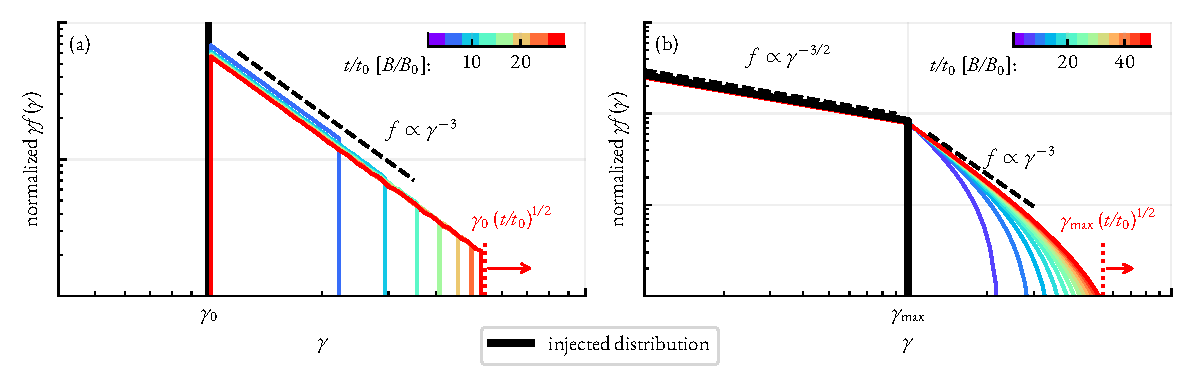
\includegraphics[width=\textwidth]{figures/ch2-reconnection/fig2.pdf}
    \caption{Temporal evolution of the particle distribution function, $f(t, \gamma)$ (see color bar), as obtained by numerically solving Equation~\eqref{eq:fsolution} with monoenergetic (panel (a)) or power law with $\gamma_{\min} \ll \gamma_{\max}$ (panel (b)) distribution functions at injection, $S$ (shown in black). In both panels, the magnetic field grows linearly with time, while the particle injection rate is assumed to be constant. All distribution functions are normalized, so that $\int f(\gamma)d\gamma = 1$. }
    \label{fig:rec-theory}
\end{figure}

In Figure~\ref{fig:rec-theory} we plot Equation~\eqref{eq:fsolution}, for two different choices for the source term, $S(t,\gamma)$. Curves with different colors correspond to different times, $t/t_0$ (and equivalently to different magnetic field strengths, $B/B_0\equiv t/t_0$), as indicated by the inset color bars. In both panels, black solid lines indicate the distribution function of injected particles.

In the simplest scenario, when particles are injected into the volume at a constant rate, $\dot{n}=\mathrm{const}$, and with the same energy $\gamma_0$ (i.e., $S(t, \gamma)=\dot{n}\delta(\gamma - \gamma_0)$), a power-law distribution function  will develop over time, namely, $f(\gamma)\propto \gamma^{p}$ with $p=-3$, extending to an evolving high-energy cutoff $\gamma_{\rm cut}=\gamma_0\left(t/t_0\right)^{1/2}$ (see Figure~\ref{fig:rec-theory}(a)). 

% This \mpet{result} is, in fact, independent of the exact compression rate, $\dot{B}$, since Equation~\eqref{eq:gammadot} relates the logarithmic derivatives of $\gamma$ and $B$.} 

We consider next a scenario where particles are injected into the compressing volume with a power-law injection spectrum at a constant rate (i.e., $S(t, \gamma)=\dot{n}\gamma^{s} H(\gamma - \gamma_{\min})H(\gamma_{\max}-\gamma)$, with $\gamma_{\rm max}\gg \gamma_{\rm min}$, where $H(\gamma)$ is the Heaviside function). This scenario is inspired by our simulation results, which will be described in detail in Section~\ref{subsec:reconnection-particles_in_plasmoids}, where particles are injected into plasmoids already pre-accelerated. The evolution of the particle distribution function in this case is illustrated in Figure~\ref{fig:rec-theory}(b), for $s=-3/2$. The shape of the distribution in the range $\gamma < \gamma_{\rm max}$ resembles the injected power law. Thus, a power-law distribution with a sharp cutoff at $\gamma_{\max}$ upon injection will be transformed into a broken power law with a sharp break at $\gamma_{\max}$, as shown in Figure~\ref{fig:rec-theory}(b). The break indicates the transition from the injected power law to a power law with an asymptotic slope $p=-3$, as expected by monoenergetic injection of particles at $\gamma_{\max}$. If the high-energy cutoff of the injected spectrum is not sharp, then a smooth transition between the two power-law segments is expected instead of the sharp break at $\gamma=\gamma_{\max}$ shown in Figure~\ref{fig:rec-theory}(b).

In this simplified model particles were confined to move in the direction perpendicular to the magnetic field, i.e., Equation~\eqref{eq:fsolution} describes the evolution of the $f(t;\gamma_{\perp})$. In our model, as we argue in Section~\ref{sec:reconnection-conserv_ad_inv}, energizations in parallel and perpendicular direction are disentangled. At the same time, for the highest-energy particles $\gamma_{\perp} \gtrsim 2\gamma_\parallel$, meaning that the cutoff and the power-law slope are well described by the evolution of $f(t;\gamma_{\perp})$.

The results will be slightly modified for the case when the energy gain in the parallel and perpendicular directions is entangled via the enforced isotropy condition.\footnote{A discussion of possible isotropization mechanisms as well as the associated timescales, can be found in Section~\ref{sec:reconnection-anisotropy}.} While Equation~\eqref{eq:fevolution} would still be applicable, the energization term, $\dot{\gamma}$, would become $\dot{\gamma} = \dot{\gamma}_{\perp} (\gamma_\perp/\gamma)+\dot{\gamma}_{\parallel} (\gamma_\parallel/\gamma)$. In the extreme case where the distribution isotropy is enforced on timescales shorter than the acceleration timescale, i.e., $\langle\gamma_\parallel\rangle/\langle\gamma_\perp\rangle=1/2$ at all times, we obtain $\dot {\gamma} = 3\sqrt{5}\dot{\gamma}_\perp/4 = 3\gamma / 4 t$, resulting in a somewhat faster acceleration rate, $\gamma_{\rm cut}\propto t^{3/4}$. However, the slope of the power-law tail will remain unchanged. 

An important remark is that the $p=-3$ power law is not universal and strictly relies on the magnetic field compression rate, $B\propto t^{\alpha}$, and the parameter $\alpha$ (which for $p=-3$ is $1$). This parameter, as will be shown in consequent sections, depends on the plasmoid growth rate and does not vary significantly (see Section~\ref{sec:reconnection-plasmoids}). So in general it is safe to assume that for realistic parameters the emerging power law will be very close to $p=-3$. 

Let us briefly recap the main results of our analytical model, which relies on the magnetic field compression and conservation of the first adiabatic invariant of particles.
\begin{itemize}
    \item Particles injected at a constant rate and with the same (relativistic) energy into an isolated volume permeated by a magnetic field whose strength is increasing linearly with time will obtain over time a power-law distribution function with slope $p=-3$ extending up to a high-energy cutoff evolving as $\propto t^{1/2}$.
    \item Particles injected at a constant rate with a power-law distribution function into the same volume will obtain over time a broken power-law distribution function with a break at the high-energy cutoff of the injection spectrum. The shape of the distribution below the break is the same as upon injection, while the  power-law segment above the break has a slope $p=-3$ and is followed by a high-energy cutoff evolving as $\propto t^{1/2}$. 
\end{itemize}

In subsequent sections we will address several assumptions that are used in the analytical model and may appear ad hoc. In Section~\ref{sec:reconnection-plasmoids} we present a theoretical model for the plasmoid interior structure that is developed based on the findings of our numerical simulations, whose setup is described in Section~\ref{sec:reconnection-setup}. We later combine the model for the plasmoid structure with the dynamics of particles within plasmoids to justify our analytical model for the evolution of the particle energy spectrum. In Section~\ref{subsec:reconnection-particles_in_plasmoids} we discuss the temporal evolution of particles injected into the plasmoid and directly compare the analytical predictions with our simulations.

% % % % % % % % % % % % % % % % % % % % % % % % % % % % % % % % % % % % 
%
% 
% % % % % % % % % SEC 3/  % % % % % % % % % % % % % % % % % % % % % % %
%
% 
% % % % % % % % % % % % % % % % % % % % % % % % % % % % % % % % % % % % 

\subsubsection{Simulation setup} 
\label{sec:reconnection-setup}
We use the electromagnetic relativistic particle-in-cell code \texttt{Tristan-MP v2},\footnote{\url{https://ntoles.github.io/tristan-wiki/}} which is a multispecies extension of the original \texttt{Tristan-MP} code \citep{2005AIPC..801..345S}. 
We perform 2D simulations of reconnection in electron--positron (pair) plasmas with zero guide field. We initialize the reconnection layer (along the $y$-direction) as a Harris sheet with length $L$. The magnetic field 
\begin{equation}
    \bm{B} = B_{\rm up} \tanh(x/\Delta) \hat{\bm{y}},
\end{equation} 
reverses at $x=0$ over a thickness $\Delta$. We choose the latter to be small enough so as to make the current sheet tearing-unstable on short timescales. For that we typically use $\Delta\approx 5\left(c/\omega_{\rm p}\right)_{\rm up}$ and $L\approx 5000\left(c/\omega_{\rm p}\right)_{\rm up}$, where $\left(c/\omega_{\rm p}\right)_{\rm up} \equiv \sqrt{m_e c^2/ 4\pi n_{\rm up} e^2}$ is the skin depth of the cold upstream plasma, which we resolve with five simulation cells, and $n_{\rm up}$ is the number density of background electrons (or positrons). Thus, even if we do not perturb the initial current sheet, it will ``break up'' starting from numerical noise with a subsequent development of the plasmoid instability. We use periodic boundaries in the $y$-direction (which is parallel to the current sheet), while in the other direction our boundaries are open with constant injection of plasma and magnetic field (for details, see \citealt{2014ApJ...783L..21S}). The energy in our simulations is not conserved to machine precision owing to the explicit nature of the numerical scheme and finite number of particles per skin depth. We thus employ eight Gaussian filter passes on deposited currents, which keeps the energy nonconservation well below the $1\%$ level. Note also that inside plasmoids the number of particles per skin depth is $\mathcal{O}(10^2)$, which further decreases the numerical noise in these regions of interest.

Upon initialization, the term $\nabla\times\bm{B}$ is balanced by the out-of-plane current, $j_z$. The magnetic pressure outside the current sheet is balanced by the particle pressure in the initial current sheet, which is provided by a hot plasma with three times higher number density compared to the number density of particles outside the layer. Because the properties of these initially hot particles in the current sheet depend on initial conditions, we exclude them from further analysis.
  
The plasma outside the layer (upstream) is cold, with a small thermal spread upon initialization ($k T_{\rm up}/m_e c^2 \equiv \Theta_e =10^{-4}$). The key parameter that characterizes the overall dynamics of the system is the magnetization of the upstream plasma, $\sigma_{\rm up}$. This quantity is a dimensionless measure of the magnetic energy available per particle and can be written as
\begin{equation}
    \label{eq:sigmaups}
    \sigma_{\rm up} = \frac{B_{\rm up}^2}{4\pi h},
\end{equation}
where $h$ is the plasma enthalpy density of the upstream plasma, including the contribution of its rest-mass energy density, i.e., 
\begin{equation}
    \label{eq:enthalpy}
    h = \rho_{\rm up}c^2\left(1 + \frac{\Gamma}{\Gamma-1} \Theta_e\right),
\end{equation} 
with $\Gamma$ being the adiabatic index of the plasma and $\rho_{\rm up}=n_{\rm up} m_e$. In the case of cold upstream plasma ($\Theta_e \ll 1$), as considered here, the enthalpy density is simply given by the rest-mass energy  density of the plasma, and the magnetization simplifies to $\sigma_{\rm up} = B_{\rm up}^2/4\pi \rho_{\rm up} c^2$. In this section of my thesis, we study reconnection in the relativistic regime (i.e., $\sups\gg 1$) and show results from two large-scale simulations with $\sups=10$ and $100$.

In general, the Larmor radius of an electron (or positron) in the upstream magnetic field, $B_{\rm up}$, can be written as 
\begin{equation}
    \tilde{r}_{L} = \gamma\beta \frac{m_e c^2}{|e| B_{\rm up}} = 
    \gamma\beta\frac{\left(c/\omega_{\rm p}\right)_{\rm up}}{\sqrt{\sups}}.
\end{equation}
where $\gamma$ and $\beta$ are the particle's Lorentz factor and three-velocity (in units of $c$), respectively.\footnote{Here the motion is assumed to be confined in the direction perpendicular to the magnetic field.} The Larmor radius, $r_L$, of particles with $\gamma=\sigma_{\rm up}\gg 1$, $\beta\approx 1$, which roughly corresponds to the energy gain assuming that particles tap the whole dissipated magnetic field energy, is
 \begin{equation}
 \label{eq:rL}
    r_{L}=\sqrt{\sigma_{\rm up}}\left(\frac{c}{\omega_{\rm p}}\right)_{\rm up}.
\end{equation}
Henceforth, we adopt $r_{L}$ as our length unit, and we quote times normalized to $r_L/c$. 

% % % % % % % % % % % % % % % % % % % % % % % % % % % % % % % % % % % % 
%
% 
% % % % % % % % % SEC 3/  % % % % % % % % % % % % % % % % % % % % % % %
%
% 
% % % % % % % % % % % % % % % % % % % % % % % % % % % % % % % % % % % % 

\section{Structure and evolution of magnetic islands}
\label{sec:reconnection-plasmoids}

\begin{figure}[htb]
    \sidebysidecaption{0.555\linewidth}{0.42\linewidth}{
        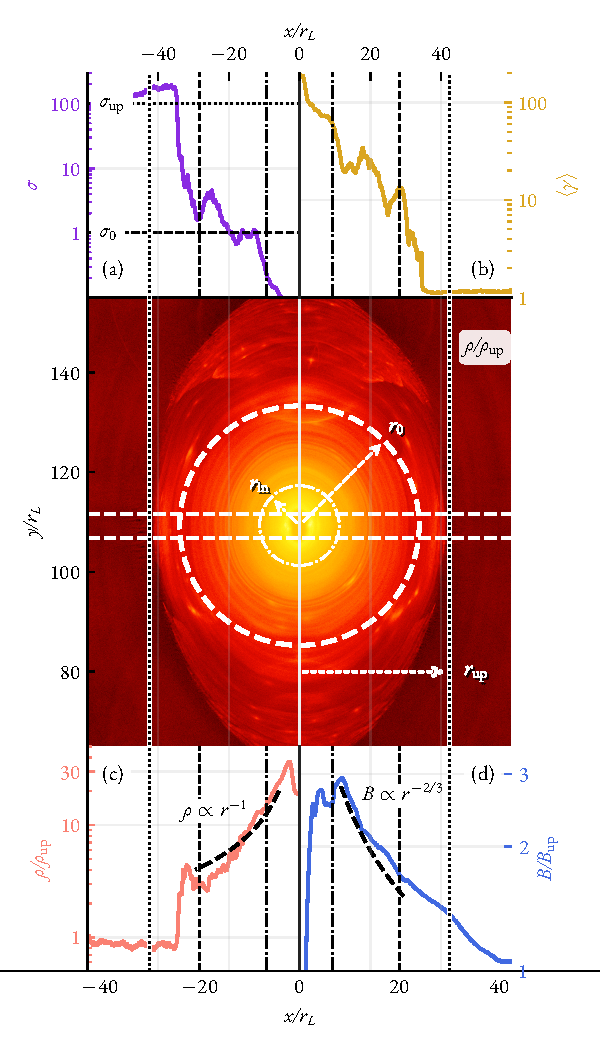
\includegraphics[width=0.95\linewidth]{figures/ch2-reconnection/fig3.pdf}
    }{
        \caption{Close-up view of a representative isolated primary plasmoid from the simulation with $\sups=100$ at time $ct/r_L=391$; this plasmoid is indicated in Figure~\ref{fig:rec-evolution} by a white solid rectangle. Color in the middle panel represents the plasma density $\rho$, in units of the upstream plasma density $\rho_{\rm up}$, in logarithmic scale (same color-coding as in Figure~\ref{fig:rec-evolution}). Three characteristic radii are also marked on the plot: $\rups$ indicates the boundary of the {\it plasmoid corona} (i.e., where the plasmoid ends and the upstream begins); $r_0$ shows the outer boundary of the {\it plasmoid shell}, where the local force balance condition is satisfied; and $\rins$ indicates the plasmoid core that contains hot unmagnetized plasma from the initial current sheet. Four peripheral panels show the radial profiles of (a) the magnetization, (b) mean Lorentz factor, (c) plasma density in units of its upstream value, and (d) magnetic field in units of its upstream value, computed along a transverse stripe passing through the plasmoid center (see horizontal dashed white lines in middle panel). In all peripheral panels, vertical lines indicate the characteristic radii marked in the middle plot. Two horizontal lines in the top left panel indicate the upstream magnetization, $\sups \gg 1$, and the effective magnetization of the plasmoid shell, $\sigma_0 \approx 1$. All plots share the same $x$-axes.}
        \label{fig:rec-plasm_example}
    }
\end{figure}

As we have postulated in the previous section, plasmoids can be thought of as compressing regions with a constantly amplifying magnetic field. They continuously accrete particles from the upstream plasma and the reconnected plasma outflows. In this section, we will study the structure of plasmoids and the plasmoid compression rate and explore the factors that determine these plasmoid properties. 

Let us take a close look at the structure of a typical isolated plasmoid in the reconnection layer. Figure~\ref{fig:rec-plasm_example} (middle panel) shows a close-up view of the plasma density structure in a typical isolated primary plasmoid, also highlighted with a solid rectangle in Figure~\ref{fig:rec-evolution} at time $ct/r_L = 391$. The four peripheral panels in the figure show 1D profiles of the magnetization\footnote{
The magnetization, $\sigma$, is computed using the local {magnetic field strength and} enthalpy density, $\sigma = B^2 / 4\pi h$, where  $h$ is defined in Equation~\eqref{eq:enthalpy} with $\Gamma\sim 4/3$ and $\Theta_e\equiv P_e/\rho_ec^2 \sim \langle\gamma\beta^2\rangle$/3.}
($\sigma$, panel (a)), mean particle Lorentz factor ($\langle\gamma\rangle$, panel (b)), mass density ($\rho$, panel (c)), and magnetic field strength ($B$, panel (d)), computed along a transverse stripe of width $5r_L$ passing through the plasmoid center (white dash-stroked stripe in middle panel). 
All panels share common $x$-axes. 

As we get closer to the plasmoid center, we can see how magnetization, $\sigma$, drops from the upstream value, $\sups$, to about $\sigma_0\sim 1$, which implies equipartition between the plasma and the magnetic field energy densities. At the same time, the plasma gets hotter towards the center (see panel (b) for $\langle\gamma\rangle$), which suggests that within the plasmoid the plasma has already been heated by magnetic energy dissipation. Both the plasma density and magnetic field strength increase compared to the upstream values as power laws of the distance from the plasmoid center (lower panels).

In primary plasmoids we can identify three regions of interest that we describe below. The central part of the plasmoid ($r < \rins$), the {\it plasmoid core}, contains typically hot unmagnetized plasma used to initialize the current sheet (see Section \ref{sec:reconnection-setup}). Because the core bears the memory of our initial conditions, it is excluded from all further analysis. The inner part of the plasmoid beyond the core (i.e., $\rins < r < r_0$), which we label as the {\it plasmoid shell}, is almost circular, and its structure is determined solely by the local force balance condition, which we will discuss later in this section. Henceforth, we use the subscript ``$0$'' to indicate physical quantities computed at the boundary of the plasmoid shell. Finally, the outer part of the plasmoid ($r_0 < r < \rups$),\footnote{$\rups$ denotes the characteristic size of the plasmoid.} which we call the {\it plasmoid corona}, is elongated along the current sheet. The corona can be thought of as a transitional layer between the inner plasmoid region and the upstream plasma where the magnetization changes rapidly (see, e.g., Figure~\ref{fig:rec-plasm_example}(a)). The coronal dynamics and structure are dictated by the plasma inflow and the time-varying properties of the upstream and current sheet. In what follows, we focus on the structure of the plasmoid shell.

Motivated by the power-law radial profiles of the magnetic field and density in the plasmoid shell (see Figure~\ref{fig:rec-plasm_example}(c) and \ref{fig:rec-plasm_example}(d)), we assume that they can both be expressed as functions of radius from the plasmoid center, $r$, and time, $t$, in the following form:
\begin{equation}
    \label{eq:radialstruct}
    B(r,t)=B_0\left(\frac{r}{r_0(t)}\right)^{-\zeta},~\rho(r,t)=\rho_0\left(\frac{r}{r_0(t)}\right)^{-\xi},
\end{equation}
where $\zeta, \xi \ge 0$, and $B_0\equiv B(r_0(t), t)$, $\rho_0\equiv \rho(r_0(t), t)$ are the time-independent boundary values of the magnetic field and density, respectively. The characteristic size of the plasmoid shell, which is proportional to the plasmoid size at all times (i.e., $r_0(t)\propto \rups(t)$), can be written as
\begin{equation}
    \label{eq:inflationrate}
    r_0(t)\propto t^\kappa,
\end{equation}
where $\kappa\ge 0$. 
Thus, at any fixed radius in the plasmoid shell, the temporal dependence of the magnetic field and plasma density can be written as $B\propto t^{\zeta\kappa}$ and $\rho\propto t^{\xi\kappa}$.

The exact value of $\kappa$ is determined by the large-scale reconnection process. By studying the growth of sufficiently large and slowly moving isolated plasmoids, like the one marked in Figure~\ref{fig:rec-evolution}, we find that
\begin{equation}
\label{eq:kappa}
    \kappa\approx 1/2 - 3/4
\end{equation}
for both $\sups = 10$ and $\sups = 100$ simulations. The exact value of the index $\kappa$ may also depend on the numerical setup and, more specifically, on the boundary conditions used. For example, \cite{2016MNRAS.462...48S} observed $\kappa\approx 1$ 
in their 2D simulations of reconnection with outflow boundary conditions in the
$y$-direction (as opposed to the periodic boundary conditions used in our simulations).

% This rate of growth can be larger for different types of boundary conditions; 

The power-law indices $\zeta$ and $\xi$ of the magnetic field and density profiles (see Equation~\eqref{eq:radialstruct}) can be predicted from the MHD force balance equation for the plasmoid shell, $\bm{j}\times\bm{B}=c{\bm \nabla} P$, assuming a polytropic EOS with adiabatic index $\Gamma$. The force balance condition yields
\begin{eqnarray}
    \label{eq:zeta}
    \zeta & = & \frac{\Gamma\sigma_0/2}{\Gamma + \Gamma\sigma_0/2 - 1}, \\
    \xi & = &  \frac{\sigma_0}{\Gamma + \Gamma\sigma_0/2 - 1} \cdot
    \label{eq:xi}
\end{eqnarray}
Here $\sigma_0$ is the effective magnetization inside the plasmoid shell, which is typically of the order of $\sigma_0\sim 1$, as illustrated in Figure~\ref{fig:rec-plasm_example}(a). For both $\sigma_{\rm up} = 10$ and $\sigma_{\rm up} = 100$ simulations, we also find typical values for the adiabatic index $\Gamma=4/3$. Substitution of these values into Equations \eqref{eq:zeta} and \eqref{eq:xi} yields
\begin{equation}
    \zeta \approx 2/3,~\text{and}~\xi \approx 1.
\end{equation}
These values are consistent with what we observe in our simulations (see, e.g., bottom panels in Figure~\ref{fig:rec-plasm_example}) and with the results of \cite{2016MNRAS.462...48S}, who reported $\zeta\approx 0.6$ and $\xi \approx 1$ (see, e.g., Appendix A of that reference).


Let us finally estimate the injection rate of particles into the plasmoid shell. At any given time, the total number of particles in the plasmoid shell can be estimated as 
\begin{equation}
    \label{eq:number_vs_time}
    N_0(t)\propto \int_{\rins}^{r_0(t)} \! \! \rho(r, t) rdr \propto r^2_0(t) \propto t^{2\kappa},
\end{equation}
where we used Equation~\eqref{eq:radialstruct} and assumed that $\rins \ll r_0(t)$ and $\xi \ne 2$ (for $\xi=2$, $N_0(t) \propto r^2_0(t) \ln [r_0(t)/\rins]$). The injection rate can be then written as
\begin{equation}
    \label{eq:injrate}
    \dot{N_0}(t)\propto r_0(t)\dot{r}_0(t)\propto t^{2\kappa-1}.
\end{equation}
For $\kappa\approx 1/2$ the injection rate of particles in the plasmoid shell is exactly constant in time, while for $\kappa\approx 3/4$ the rate scales as $t^{1/2}$. Equation~\eqref{eq:number_vs_time} also implies that the mean density inside the plasmoid shell, $\langle\rho\rangle \propto N_0(t)/r^2_0(t)$, is constant (or scales weakly with time), regardless of the exact value of $\kappa$.  

It is worth noting that the results presented in this section do not directly depend on the upstream conditions, such as the upstream magnetization. The reason is that the interior of the plasmoid -- the plasmoid shell -- contains magnetized plasma that has already been ``reprocessed'' by reconnection. The magnetic flux loops in the plasmoid shell do not bear the memory of the conditions in the unreconnected plasma. They are in force balance with the relativistically hot plasma in the plasmoid shell. The radial profile of the magnetic field essentially depends on the plasma EOS. The growth of the magnetic flux in the plasmoid interior, which is adiabatically slow, is dictated by the global reconnection rate. The reconnection rate, which can also be thought of as the inflow velocity from the upstream, is ubiquitous for systems with low enough-resistivity, and for relativistic plasmas it is equal to $v_{\rm in}\sim 0.1c-0.2c$. 

Summarizing, the key result of this section is that the structure and evolution of the plasmoid shell are described by three dimensionless numbers: the power-law indices of magnetic field and plasma density profiles $\zeta$ and $\xi$, respectively, defined in Equation \eqref{eq:radialstruct}, and the plasmoid growth rate $\kappa$ defined in Equation~\eqref{eq:inflationrate}. The first two are set by the force balance in the plasmoid shell and can be obtained assuming a simple polytropic EOS of the relativistically hot plasma in the plasmoid. The third one, however, is determined by the large-scale reconnection process and has to be determined empirically (from the simulations).

% % % % % % % % % % % % % % % % % % % % % % % % % % % % % % % % % % % % 
%
% 
% % % % % % % % % SEC 4/  % % % % % % % % % % % % % % % % % % % % % % %
%
% 
% % % % % % % % % % % % % % % % % % % % % % % % % % % % % % % % % % % % 

\section{Evolution of particles trapped inside the magnetic islands}
\label{subsec:reconnection-particles_in_plasmoids}

\begin{figure}[htb]
    \centering
    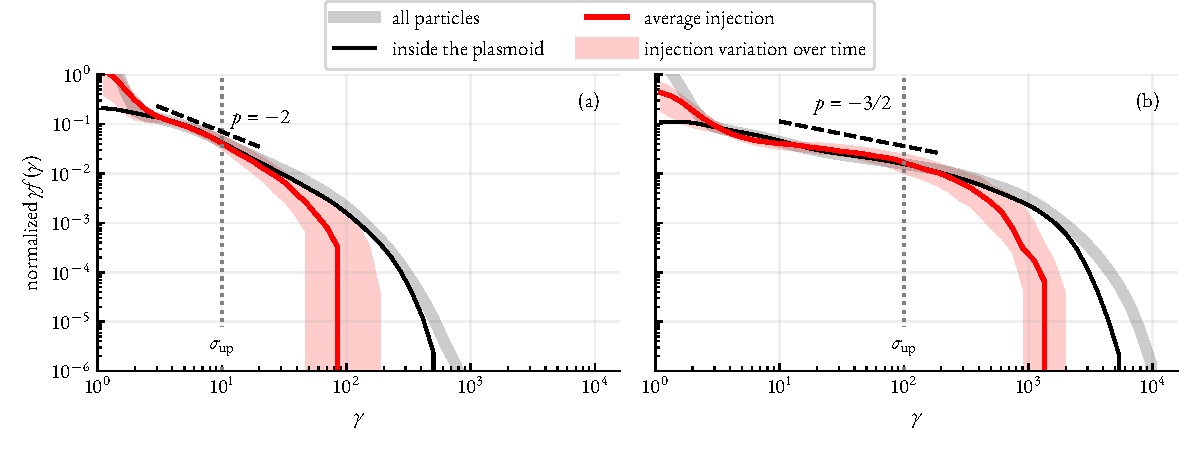
\includegraphics[width=\textwidth]{figures/ch2-reconnection/fig4.pdf}
    \caption{Particle distribution functions, $f(\gamma)$, compensated by $\gamma$, from  the $\sigma_{\rm up}=10$ (panel (a)) and $\sigma_{\rm up}=100$ (panel (b)) simulations. The time-averaged injection spectra are shown with a red line, while the variation of injected distribution over time is illustrated by the transparent red band. For panel (a) the averaging period is $1300<ct/r_L<2000$, and for panel (b) it is $420 < ct/r_L < 620$. Black solid lines show the distribution function of all the particles in the plasmoid, while the thick gray line represents the distribution function of all the particles in the simulation domain; both of these lines are computed at the end of the quoted time period. For comparison purposes, all distribution functions are normalized so that $\int f(\gamma)d\gamma=1$. In these plots it is evident that the distribution function of the plasmoid as a whole (black line) extends farther than the distribution of the injected particles (red line).}
    \label{fig:rec-injspec}
\end{figure}
In this section, we focus on the evolution of particles upon their injection into plasmoids, while making use of our results about the plasmoid interior structure and its evolution.

There are two main channels for particle injection into plasmoids from the cold upstream region. First, particles can be accreted directly onto a plasmoid as they are carried toward the current sheet by converging magnetic field lines. These particles typically have low energies upon entering a plasmoid (i.e., $\gamma \sim 1$), as they have never interacted with the current sheet before. Alternatively, particles from the upstream region can interact with the current sheet first before entering a plasmoid. In this case, the injected particle population is already pre-accelerated either by the electric field at an X-point \citep{2001ApJ...562L..63Z, 2003ApJ...586...72L, 2008ApJ...682.1436L} or by the motional electric field via the so-called ``slingshot'' Fermi-like mechanism \citep{2006Natur.443..553D, 2014PhRvL.113o5005G, 2015ApJ...806..167G}. Thus, at any given time the injection spectrum of a plasmoid is expected to be a superposition of the ``cold'' component directly coming from the upstream and a ``hot''  pre-accelerated component inflowing from the current sheet. 

Time-averaged spectra of particles injected\footnote{
We compute these spectra using particles near the boundary of plasmoid. The injection spectra are averaged over the time span mentioned in the caption of Figure~\ref{fig:rec-injspec}.} into a typical isolated plasmoid from our simulations are shown in Figure~\ref{fig:rec-injspec} (red lines). Panels (a) and (b) show results for $\sups=10$ and $\sups=100$, respectively. The plasmoid, whose spectrum is displayed in panel (b), is also highlighted in Figure~\ref{fig:rec-evolution} (white rectangle). In both panels, the average injection spectrum can be described by a power law (i.e., $f(\gamma)\propto\gamma^{p}$ with $p\sim -2$ for $\sups=10$ and $p\sim -1.5$ for $\sups=100$). This power law typically extends up to Lorentz factors of several $\sups$. We also note that the injection spectrum does not vary much with time, as shown  by the red colored band in Figure~\ref{fig:rec-injspec}. This is true except for times very early in a plasmoid's lifetime, when small variations in the amount of mass accreted via the adjacent current sheets and the upstream plasma can significantly affect the overall spectral shape (not explicitly shown here). 

The spectrum computed using all particles trapped within the plasmoid at a given time (thin black line) does not match the injection spectrum, as shown in Figure~\ref{fig:rec-injspec}. More specifically, the energy spectrum of particles contained in the plasmoid appears to be shifted to higher energies compared to the injected spectrum (compare black and red solid lines). These results suggest the presence of an acceleration mechanism operating within the isolated plasmoids that is responsible for pushing the injected particles to even higher energies than those achieved via other processes prior to injection. 

Identifying the process that energizes particles after their injection into plasmoids is also important for understanding the formation of the particle spectrum from the reconnection layer as a whole. The reason is that, at times when the current sheet is dominated by large plasmoids (see $ct/r_L > 300$ in Figure~\ref{fig:rec-evolution}), the majority of particles (including the most energetic ones) are ultimately trapped inside magnetic islands. This is exemplified in Figure~\ref{fig:rec-injspec}, where the particle spectrum from the whole simulation box (thick gray line) -- normalized to the total number of particles -- is compared against that of a single plasmoid (thin black line). When both spectra are normalized to their total number of particles, as done in this figure, the particle spectra for $\gamma \gg 1$ fall on top of each other, except for the highest-energy part. We note also that some of the freshly injected particles (distribution of which is shown by red color) may have already undergone this secondary energization in smaller plasmoids that merged into the bigger plasmoid under study. This, in part, can explain the variability in the particle injection spectrum.

\subsubsection{Particle evolution in the plasmoid shell}
\label{sec:part-evol}
\begin{figure}[htb]
    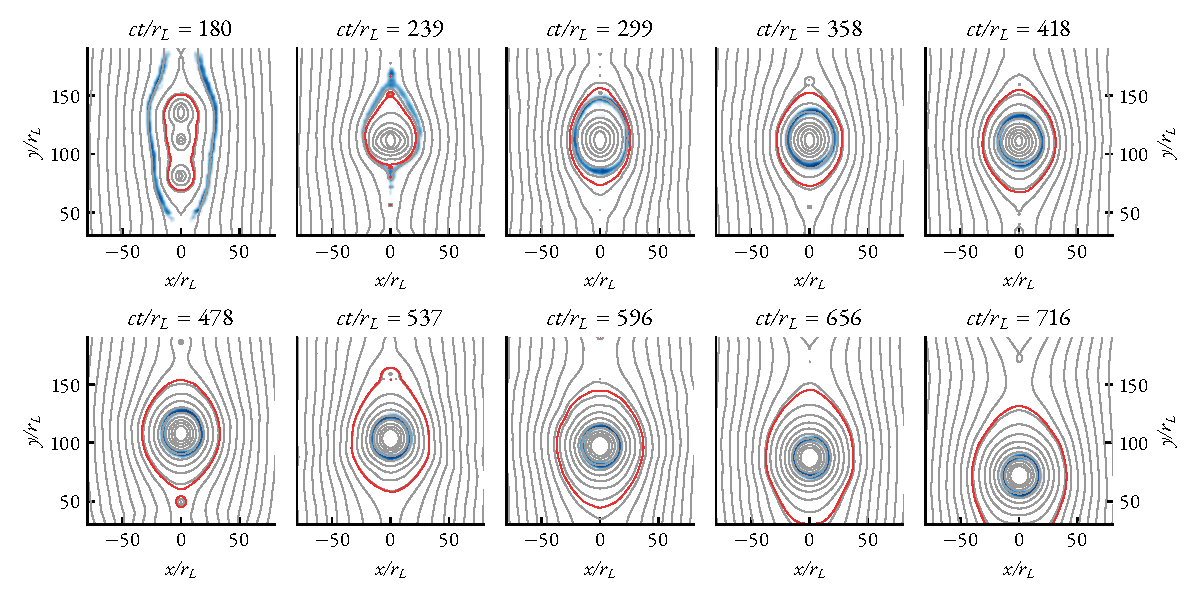
\includegraphics[width=\textwidth]{figures/ch2-reconnection/fig5.pdf}
    \caption{
        Snapshots from the $\sups=100$ simulation focused on the same primary plasmoid highlighted in Figure~\ref{fig:rec-evolution} with solid lines. The plasmoid boundary is highlighted with a solid red line. Gray lines are the isocontours of the magnetic vector potential, $A_z$. A population of $\sim 10^4$ particles (shown in blue) is initially frozen to a magnetic field line (see top left panel). The particles enter the plasmoid roughly at the same time ($239 < ct/r_L < 299$) and are later carried toward the center of the plasmoid. An animation showing the evolution of various physical quantities for the same particle population can be found at the following link: \url{https://youtu.be/UJsjoIieLm0}. 
    }
    \label{fig:rec-layerevol}
\end{figure}
In this section, we track a population of about $10^4$ particles from the $\sups=100$ simulation that enter the isolated primary plasmoid shown in Figure~\ref{fig:rec-evolution} (white rectangle) at roughly the same time (around $ct/r_L\approx 300$) and follow their evolution as they are carried inward to its center. This is illustrated in Figure~\ref{fig:rec-layerevol}, where different panels show different snapshots of the selected plasmoid (its boundary is indicated with a red contour) and the tracked particle population (shown in blue). With the help of these particles, we can not only study the acceleration taking place directly inside the plasmoid but also map the plasmoid structure in Lagrangian terms (i.e., in the frame comoving with the fluid element). Because particles are well magnetized, as their gyroradii are much smaller than the shell size (we will inspect this further in Section~\ref{sec:reconnection-conserv_ad_inv}), their evolution also tracks the magnetic field line on which they started in the upstream.

In Figure~\ref{fig:rec-layerevol} the particles (shown in blue) are frozen into converging magnetic field lines. At around $ct/r_L\sim 200$ the flux loop reconnects, and some of the particles are exposed to the X-point and are pre-accelerated in the current sheet, forming the injection spectrum shown in red color in Figure~\ref{fig:rec-injspec}(b). Around $ct/r_L\sim 300$ particles cross the plasmoid boundary entering the plasmoid corona but quickly converge into the plasmoid shell, as the flux loop to which they are frozen circularizes (we define the coronae and shells of plasmoids in Section~\ref{sec:reconnection-plasmoids}).

In the plasmoid shell, particles start their adiabatically slow descent toward the plasmoid core ($ct/r_L > 300$). Plasma in the plasmoid shell is also frozen to the converging concentric magnetic field lines, each of which can be thought of as a circle with a time-varying radius $\Rlg(t)$. Henceforth, calligraphic capital letters will be used to denote variables in Lagrangian terms. The total mass enclosed within a circle of radius $\Rlg$ is constant in time, as particles cannot move across concentric magnetic field lines. This condition yields
\begin{equation}
    \label{eq:rL_vs_t}
    \Rlg(t)\propto t^{-\kappa\xi/(2-\xi)},
\end{equation}
where $\xi$ and $\kappa$ are defined in Equations~\eqref{eq:radialstruct} and \eqref{eq:inflationrate}, respectively. For $\xi\approx 1$, as found in our simulations (see Section~\ref{sec:reconnection-plasmoids}), the expression above simplifies to $\Rlg \propto t^{-\kappa}$. The magnetic field strength at the particle location, $\Blg$, can be estimated by substituting $\Rlg(t)$ into Equation~\eqref{eq:radialstruct},
\begin{equation}
    \label{eq:BL_vs_t}
    \Blg(t)\propto t^{2\kappa \zeta/(2-\xi)}\propto t^{4\kappa/3},
\end{equation}
where we assumed $\xi\approx 1$ and $\zeta\approx 2/3$ to derive the second scaling relation in the equation above.


\begin{figure}[tb]
    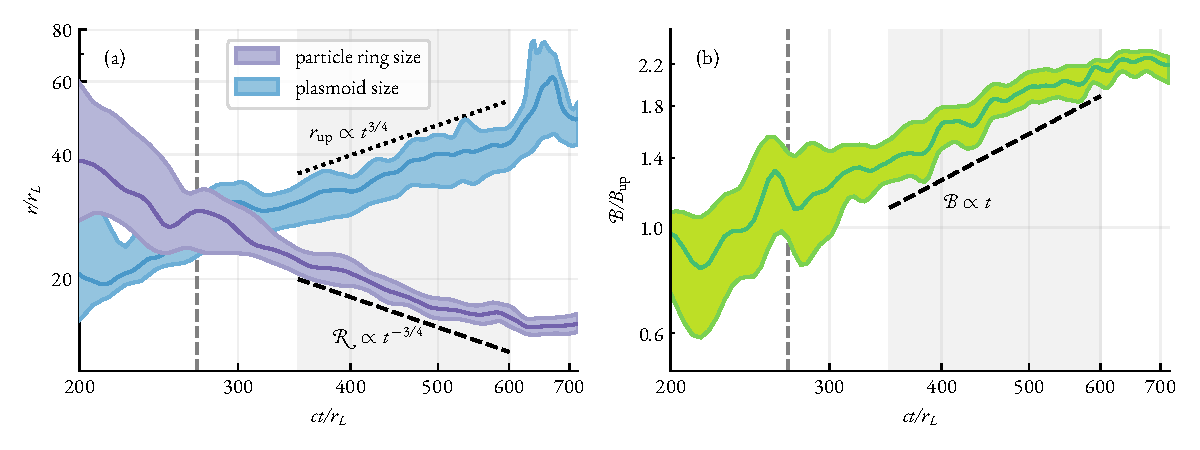
\includegraphics[width=\textwidth]{figures/ch2-reconnection/fig6.pdf}
    \caption{Temporal evolution of the distance from the plasmoid center, $\Rlg$ (panel (a)), and the magnetic field strength at the particle location, $\Blg$ (panel (b)), for the generation of particles shown in Figure~\ref{fig:rec-layerevol} in blue. Colored bands represent the spread in values within the particle population, while the solid lines show the median value. In panel (a) we also show the evolution of the plasmoid size, $\rups$, as a function of time; the spread, in this case, originates from the fact that the outer boundary of this plasmoid is actually elliptical. The vertical dashed line indicates the time when particles enter the plasmoid, and the gray band at $350<ct/r_L<600$ corresponds to the time when particles are within the contracting shell while the plasmoid remains isolated. As particles spiral down toward the center of the plasmoid ($\Rlg(t)$), the plasmoid itself grows ($r_{\rm up}(t)$), and the magnetic field strength that particles experience grows with time ($\Blg(t)$). At $ct/r_L\sim 600$ the ring of particles reaches the unmagnetized inner core of the plasmoid, where the MHD balance condition we discussed no longer holds, which is why the growth in $\Blg$ halts.}
    \label{fig:rec-layer_r_b}
\end{figure}
We then compare the empirical relations for $\Rlg(t)$ and $\Blg(t)$ with the scalings derived directly from our numerical simulations. In Figure~\ref{fig:rec-layer_r_b} we show how the distance from the plasmoid center (purple band in panel (a)) and the magnetic field strength (panel (b)) evolve with time for the same generation of particles shown in Figure~\ref{fig:rec-layerevol}. In both panels, solid lines correspond to the median value of the displayed variable, and the colored band indicates the spread in values within the tracked particle population. As particles move toward the plasmoid center, the corresponding spread in $\Rlg$ and $\Blg$ becomes smaller as the plasmoid shell is circularized. In panel (a), we also plot the radius of the plasmoid boundary, $\rups$, as a function of time (blue band). For this particular plasmoid, we find $\rups\propto t^{3/4}$ or $\kappa\approx 3/4$. As particles are advected by the magnetic loop toward the plasmoid center, their distance decreases with time as $\Rlg\propto t^{-3/4}$, while the magnetic field at the particle location grows roughly linearly with time, $\Blg\propto t$. This is in a good agreement with the analytical scalings of Equations~\eqref{eq:rL_vs_t} and \eqref{eq:BL_vs_t} for $\kappa=3/4$. Notice that the magnetic field strength $\mathcal{B}$ is measured in the lab frame, whereas to compare with our analytical estimations we need to measure it in the frame comoving with the plasmoid (i.e., moving with an $\boldsymbol{E}\times\boldsymbol{B}$ drift velocity). However, since the plasmoid we consider is large and slow, any corrections to our measurements are negligible.

Summarizing, there are two effects acting together to build up the linear increase of the magnetic field strength with time experienced by a particle population after its injection into a plasmoid shell. First, the plasmoid interior gets compressed, and the magnetic field at a fixed distance from its center gets amplified. Second, particles ``sink'' toward the center of the plasmoid, experiencing an increasingly stronger magnetic field. 

% \subsection{Evolution of particle energy in the  plasmoid shell}
\subsection*{Conservation of adiabatic invariants}
\label{sec:reconnection-conserv_ad_inv}
We now focus on the energization of particles after they enter into the plasmoid, using the same sample of tracked particles as in the previous section. In Figure~\ref{fig:rec-layer_gam_mu}(a) we plot the evolution of the mean energy of particles, $\langle \gamma\rangle$, as a function of time. For $ct/r_L \gtrsim 290$, i.e., after the particles have sunk into the plasmoid shell (see also Figure~\ref{fig:rec-layerevol}), the growth of the mean energy is sublinear with time. The same applies for the high-energy cutoff of the particle energy spectrum, namely, $\gamma_{\rm cut} \propto t^{1/2}$, in agreement with the results of PS18. The cutoff is found using a similar approach to that in \cite{2015ApJ...809...55B},
\begin{equation}
    \gamma_{\rm cut} = \frac{\int \gamma^{\alpha} f(\gamma)d\gamma}{\int \gamma^{\alpha - 1} f(\gamma)d\gamma},
\end{equation}
where the parameter $\alpha$ is empirically chosen to be $3$. This formula allows one to be agnostic to the exact power-law slope, while roughly estimating the position of the energy cutoff.

In Figure~\ref{fig:rec-layer_gam_mu}(a) we also plot the temporal evolution of the Lorentz factor of the particle motion perpendicular ($\langle\gamma_\perp\rangle$) and parallel ($\langle\gamma_{\parallel}\rangle$) to the magnetic field, averaged over the tracked particle population. We define $\gamma_{\parallel}$ and $\gamma_{\perp}$ of a single particle as
\begin{equation}
    \gamma_{\parallel} = \sqrt{1+u_{\parallel}^2},~\text{and}~\gamma_{\perp} = \sqrt{1+u_{\perp}^2},
\end{equation}
where $u_{\parallel}$ and $u_\perp$ are the parallel and perpendicular components of the particle's dimensionless 4-velocity with respect to the local magnetic field. As in PS18, we find that $\langle \gamma\rangle \approx \langle\gamma_{\perp}\rangle \sim 2 \langle\gamma_{\parallel}\rangle$. This suggests that inside the plasmoid shell the pressure\footnote{We define pressure components as the flux of the corresponding momentum components, $P_i\propto \langle\gamma_i\beta_i^2\rangle \approx \langle\gamma_i\rangle$, because $\beta_i\approx 1$.} is almost isotropic, namely $P_{\perp}\approx \rho c^2\langle\gamma_{\perp}\rangle \approx 2 \rho c^2 \langle\gamma_{\parallel}\rangle \approx 2P_{\parallel}$.


\begin{figure}[htb]
    \centering
    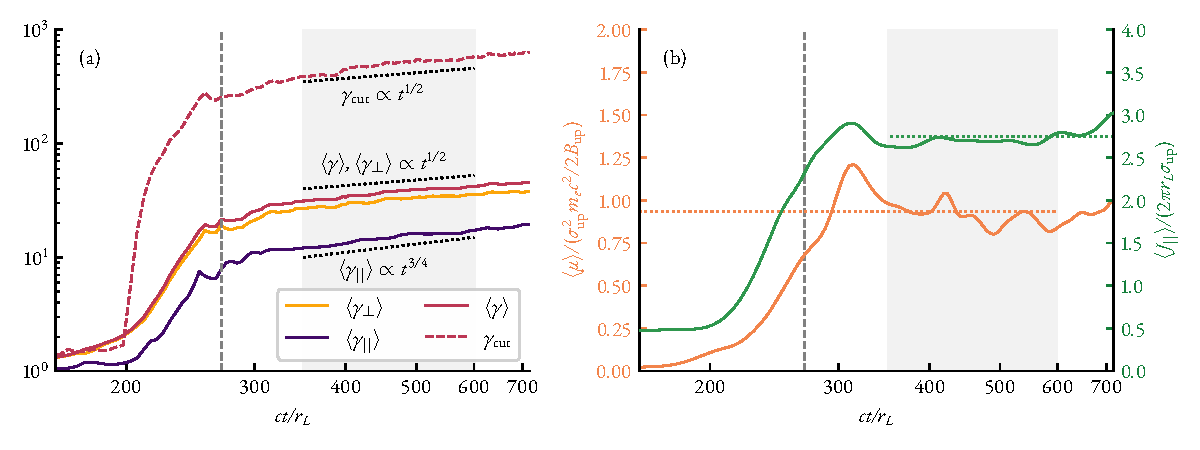
\includegraphics[width=\textwidth]{figures/ch2-reconnection/fig7.pdf}
    \caption{(a)
    Temporal evolution of the particle Lorentz factor $\langle\gamma\rangle$, and the Lorentz factor of the particle motion perpendicular ($\langle\gamma_\perp\rangle$), and parallel ($\langle\gamma_{\parallel}\rangle$) to the magnetic field (see inset legend), averaged over the particle population identified in Figure~\ref{fig:rec-layerevol}. The dashed colored line shows the evolution of the cutoff Lorentz factor of the particle energy spectrum, computed as described in Section~\ref{sec:reconnection-conserv_ad_inv}. (b) Temporal evolution of the population averaged adiabatic invariants $\mu$ and $J_\parallel$ (defined in Equations (\ref{eq:mu}) and (\ref{eq:Jpar}), respectively) for the same population of particles as in panel (a). $\langle\mu\rangle$ is normalized to $m_e \sups^2 c^2/2B_{\rm up}$, i.e., the magnetic moment of particles with $\gamma_\perp\sim \sups$ in the upstream field $B_{\rm up}$; $\langle J_\parallel\rangle$, on the other hand, is normalized to $\sups r_L$, i.e., the mirror invariant for a particle with $\gamma_\parallel\sim\sups$ trapped in a circular region of radius $r_L$. These quantities share the same $x$-axis with different $y$-axes on the left and right highlighted with corresponding colors; dotted horizontal lines indicate their average values after $ct/r_L=300$.
    In both panels, the gray dashed vertical line shows the moment when particles enter the plasmoid, and the gray band $350<ct/r_L<600$ corresponds to the time when particles are within the contracting shell while the plasmoid remains isolated. As wee see from panel (a), both the parallel and the perpendicular components of particle momenta grow with time. Since particles are well magnetized within the plasmoid shell ($ct/r_L>300$), this energization is caused by the conservation of adiabatic invariants shown in panel (b).}
    \label{fig:rec-layer_gam_mu}
\end{figure}

PS18 proposed that the conservation of the first adiabatic invariant, together with the magnetic field amplification due to plasmoid compression, is responsible for the slow and steady energy increase of particles contained within plasmoids. Our results confirm this physical interpretation, as illustrated in  Figure~\ref{fig:rec-layer_gam_mu}(b),
where we plot the magnetic moment (orange band)
\begin{equation}
\label{eq:mu}
    \mu=m_e c^2\frac{\gamma_\perp^2-1}{2 \Blg},
\end{equation} 
as a function of time for all the particles highlighted in Figure~\ref{fig:rec-layerevol}. In the equation above, $\mathcal{B}$ is computed along the particle trajectory (see also Figure~\ref{fig:rec-layer_r_b}(b)).

Soon after the particles enter the plasmoid (dashed gray line), their magnetic moment is, to a good approximation, conserved; the median value for the particle population (solid red line) is almost constant, and the variance (indicated by the width of the colored band) is much smaller than at earlier times. From the invariance of the magnetic moment ($\mu = \mathrm{const}$) and the magnetic field increase with time (see Equation \eqref{eq:BL_vs_t}) it follows that
\begin{equation}
    \gamma_{\perp}\propto \Blg^{1/2}\propto t^{1/2},
\end{equation}
where we used $\kappa=3/4$ to obtain the scaling with time. In Figure~\ref{fig:rec-layer_gam_mu}(b) we also plot the second adiabatic invariant of the particles (green band)
\begin{equation}
\label{eq:Jpar}
    J_{\parallel}=\oint p_{\parallel}dl_{\parallel} \propto \gamma\beta_{\parallel}\Rlg\approx
    \gamma_{\parallel}\Rlg,
\end{equation}
assuming that particles have $\beta_\parallel\approx 1$, and find that $J_{\parallel}\approx \mathrm{const}$ for $ct/r_L \gtrsim 300$. This conservation (not discussed in PS18) yields
\begin{equation}
    \gamma_{\parallel}\propto 1/\Rlg(t)\propto t^{3/4}.
\end{equation}
where we used Equation~\eqref{eq:rL_vs_t} with $\xi=1$ and $\kappa=3/4$. Thus, combining the conservation of the first two adiabatic invariants of the particles with the growth of the (Lagrangian) magnetic field strength, we can explain the scalings of $\langle \gamma_{\parallel}\rangle, \langle\gamma_{\perp}\rangle$ from our simulations (Figure~\ref{fig:rec-layer_gam_mu}(a)). For the the nonrelativistic version of these relations for $P_\perp(t)$ and $P_\parallel(t)$, we refer the reader to  \cite{2017PhPl...24f2906M}.

We discuss next the conditions for conservation of $\mu$ and $J_{\parallel}$ and check whether they are indeed satisfied in our simulations. The first adiabatic invariant is conserved if the particle gyration timescale ($\omega_g^{-1}$) is much shorter than the characteristic timescale for the change of the magnetic field ($\Blg/\dot{\Blg}$). The particle gyration timescale in the plasma shell (see blue ring in Figure~\ref{fig:rec-layerevol}) can be written as
\begin{equation}
    \omega_g^{-1} = \frac{B_{\rm up}}{\Blg}\cdot
        \frac{\langle\gamma\rangle}{\sups}\cdot
        \frac{r_L}{c}
    \sim \mathcal{O}(1) \frac{r_L}{c},
\end{equation}
where we assumed that $\langle\gamma\rangle\sim\sups$ and $\Blg\sim B_{\rm up}$ (see Figures \ref{fig:rec-layer_gam_mu} and \ref{fig:rec-layer_r_b}(b), respectively).
The timescale for the change of the magnetic field can be written as
\begin{equation}
    \frac{\Blg}{\dot{\mathcal{B}}}\sim \mathcal{O}\left(10^2\right) 
        \frac{r_L}{c} \gg \omega_g^{-1},
\end{equation}
as suggested by the results shown in Figure~\ref{fig:rec-layer_r_b}(b). Thus, the conservation of the first adiabatic invariant is satisfied inside the plasmoid shell. 

The second adiabatic invariant, also known as the {\it mirror invariant}, is conserved if the time to cross the system in the direction parallel to the magnetic field  is much shorter than the characteristic timescale for the change of that dimension ($\Rlg/\dot{\Rlg}$). The former timescale can be approximated by $2\pi \Rlg/c$, assuming that particles move along magnetic field lines with $\beta_\parallel \approx 1$. From Figure~\ref{fig:rec-layer_r_b}(a), we find order-of-magnitude estimates for both timescales, which read 
\begin{equation}
    \frac{\Rlg}{\dot{\Rlg}}\sim \mathcal{O}\left(10^2\right) \frac{r_L}{c},
    ~\text{while}~
    \frac{\Rlg}{c} \sim \mathcal{O}(10) \frac{r_L}{c}.
\end{equation}
Thus, the second adiabatic invariant is also conserved within a typical isolated plasmoid.

Let us also check that the particles can indeed be confined within the plasmoid during the energization process. On average, the Larmor radius of particles descending in the plasmoid shell can be written as $\tilde{r}_L \sim (\langle\gamma\rangle/\sups)(B_{\rm up}/\Blg)r_L \sim \mathcal{O}(1)r_L$, which is much smaller than the plasmoid size, $\rups \sim \mathcal{O}(10\text{-}10^2) r_L$ (see  Figure~\ref{fig:rec-layer_gam_mu}(a)). This suggests that most of the energetic particles are trapped within the plasmoid. In fact, as particles sink toward the plasmoid core, they get increasingly more magnetized;  their Larmor radii decrease, since the magnetic field strength grows faster than the particle energy, namely, $\langle\gamma\rangle\propto t^{1/2}$, whereas $\Blg\propto t$, which leads to $\tilde{r}_L\propto t^{-1/2}$.

\subsubsection{Comparison to analytical model}
\begin{figure}[htb]
    \centering
    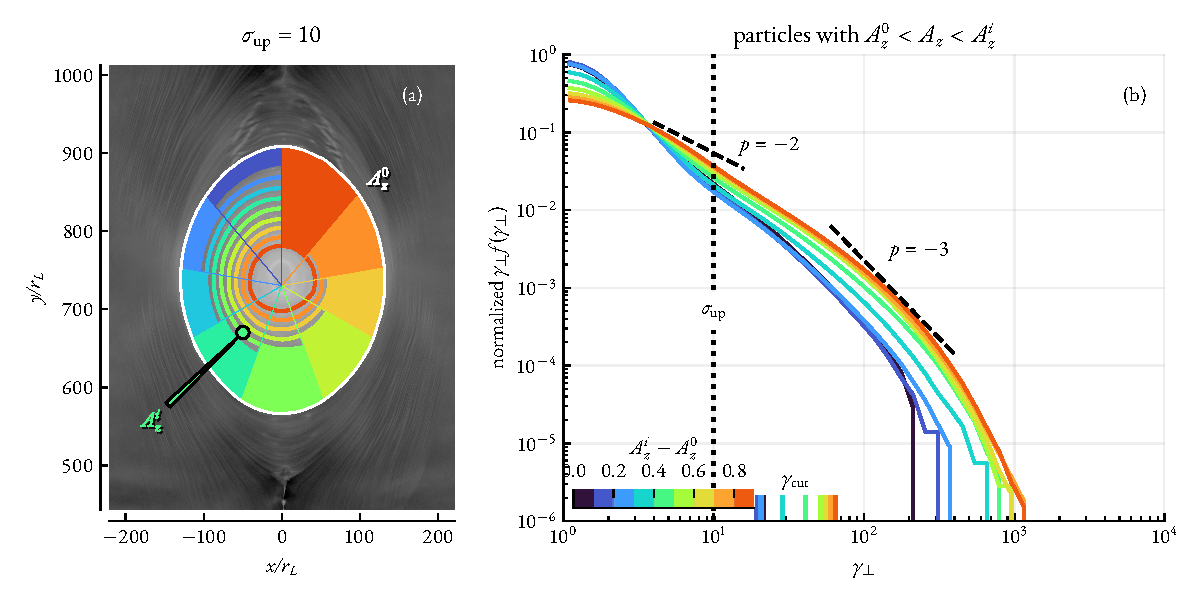
\includegraphics[width=0.75\textwidth]{figures/ch2-reconnection/fig8_1.pdf}
    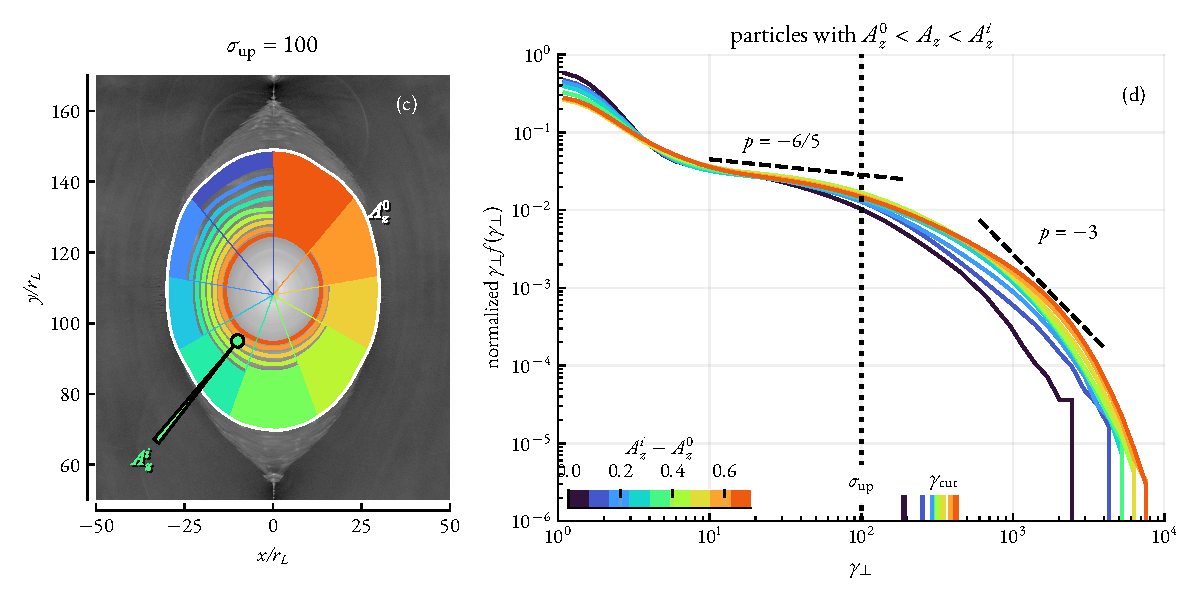
\includegraphics[width=0.75\textwidth]{figures/ch2-reconnection/fig8_2.pdf}
    \caption{(a, c) Contours of the magnetic vector potential, $A_z$, are shown with colored lines. Rings with $A_z^0 < A_z < A_z^i$ are marked using colored sectors to guide the eye. Contours are overlaid on the plasma density shown in gray from our $\sups=10$ (top) and $100$ (bottom) simulations. The white line indicates the plasmoid boundary $A_z^0$. (b, d) Distribution functions (in perpendicular direction to the magnetic field, $f(\gamma_\perp)$) of particles belonging to different rings; blue curves correspond to the outermost region, while yellow/red curves are for the entire plasmoid (except for the innermost core). Colored vertical dashes represent the corresponding cutoff energies, computed as described in Section~\ref{sec:reconnection-conserv_ad_inv}. Distribution functions are computed for the whole ring defined by $A_z^0 < A_z < A_z^i$.}
    \label{fig:rec-layers_df}
\end{figure}
In this section, we compare the predictions of our analytical model about the particle energy spectrum with the results of two simulations of reconnection with $\sups=10$ and $\sups = 100$.

First, we select an isolated plasmoid and partition it into several concentric disks defined by equally spaced contours of the vector potential, $A_z$. This is shown in panels (a) and (c) of Figure~\ref{fig:rec-layers_df}, where the $i$-th colored disk is defined by $A_z^0 < A_z < A_z^i$, and the white solid line represents the plasmoid boundary $A_z^0$. Disks are chosen in such a way that the $i$th disk contains all the $(i-1)$th, $(i-2)$th , ..., $0$th disks forming an onion structure, with the largest (red) disk containing all the other ones. We then pick particles from each of these disk regions and compute their distribution functions in the direction perpendicular to the local magnetic field, i.e., $f(\gamma_\perp)$. These are displayed in panels (b) and (d) of the same figure. For comparison purposes, all distribution functions are normalized to the total particle number of each region.

The distribution function of each disk is composed of multiple particle ``generations,'' namely, particles that were injected into the compressing plasmoid at different times. In general, particles from the outer regions (blue and green colored regions) have spent less time within the plasmoid than particles residing in the inner regions (orange and red colored regions). The difference in the particle residence time within the compressing plasmoid is reflected in the distribution functions extracted from different regions. This is illustrated in panels (b) and (d) of Figure~\ref{fig:rec-layers_df}, where we see that the energy spectra of particles from regions closer to the plasmoid center (orange and red curves) are systematically shifted to higher Lorentz factors compared to the spectra of particles from the outer regions (blue curves). Similarly, the cutoff Lorentz factor (also marked with vertical dashes in both panels) of the distribution function from the outer regions is lower and closer to $\sups$, as expected for the injection particle spectrum (see also Figure~\ref{fig:rec-injspec}). Moreover, the spectral shape is roughly the same among different disk regions, suggestive of an energization process that acts upon particles of all energies similarly, like adiabatic compression. 

The distribution functions from both simulations can be phenomenologically described as smooth broken power laws  with a high-energy exponential cutoff. The low-energy part of the spectrum has the slope of the injected energy spectrum, which depends on $\sups$. On the contrary, the high-energy part of the spectrum can be roughly described as a power law with $p\approx -3$ for both values of upstream magnetization. The steep power-law segment can be easily mistaken for an exponential cutoff because of the often limited energy range this spans. Without prior expectation for the existence of this steep power law, it is no surprise that previous studies did not report this. It is also worth emphasizing that for simulations with $\sups \lesssim 10$, where the X-point acceleration predicts steep particle spectra ($p<-2$), the robust identification of the $p=-3$ power-law tail is very difficult.

\subsubsection{Secondary energization timescale}

% Let us also make some simple estimations for the rate of plasmoid compression, which is directly related to the rate of secondary particle acceleration. 

% The magnetic field energy per unit time \mpet{and unit length in the $z$ direction that is} advected by the inflowing plasma into the current sheet is equal to
% \begin{equation}
%     W_{\rm in} \approx \frac{B_{\rm up}^2}{8\pi}v_{\rm in} \rups.
% \end{equation}
% \mpet{To derive the expression above we considered only a small region of characteristic length $\rups$ along the current sheet ($y$-direction).}
% % of the size of one particular plasmoid. 
% Some fraction of this magnetic energy is dissipated in the current sheet and directly deposited into particle energy, while the rest is carried into the plasmoid by the accreting plasma. We assume that the increase of the magnetic field energy contained within the plasmoid (due to both compression and plasmoid growth) is proportional to the magnetic energy inflow. Assuming $B \sim B_{\rm up}$ and $r\sim \rups$, we can then find the plasmoid growth rate (similar to~\citealt{2016MNRAS.462...48S})

The timescale for magnetic field compression in Lagrangian terms is $\mathcal{B} / \dot{\mathcal{B}}$. Since $\mathcal{B} = B(\mathcal{R}(t), t)$, from Equation~\eqref{eq:radialstruct} we see that this timescale is also directly related to the timescale of plasmoid growth
\begin{equation}
    \label{eq:acctimescale}
    \frac{\mathcal{B}}{\dot{\mathcal{B}}} \sim \frac{\rups}{\dot{r}_{\rm up}} \sim \frac{\rups}{v_{\rm in}},
\end{equation}
where $v_{\rm in}$ is the reconnection rate (this result is similar to~\citealt{2016MNRAS.462...48S}). This timescale is also a proxy for the secondary acceleration timescale $t_{\rm sec} = \gamma / \dot{\gamma}$, as the secondary acceleration is a direct consequence of the compression of plasmoid interior. Relation~\eqref{eq:acctimescale} implies that the timescale for plasmoid compression (and thus secondary particle acceleration) becomes longer as the plasmoid grows over time. For the particular case shown in Figure~\ref{fig:rec-layerevol}, where we can take $r_{\rm up}\sim 50r_L$ and $v_{\rm in}\sim 0.1 c$, we find that $t_{\rm sec}\sim 500r_L / c$, which roughly corresponds to the acceleration timescale inferred by Figure~\ref{fig:rec-layer_gam_mu}(a) (characteristic timescale for the growth of $\langle\gamma\rangle$ from $\sim 200$ to $\sim 400$).

% % % % % % % % % % % % % % % % % % % % % % % % % % % % % % % % % % % % 
%
% 
% % % % % % % % % SEC 5/  % % % % % % % % % % % % % % % % % % % % % % %
%
% 
% % % % % % % % % % % % % % % % % % % % % % % % % % % % % % % % % % % % 

\section{Discussion \& summary}
\label{sec:reconnection-discussion}

The standard picture for particle acceleration in relativistic reconnection is that particles get energized at the X-points and in the current sheet before being ultimately trapped inside  plasmoids, where they do not undergo any further energization. However, our study shows that this standard picture is not correct. In fact,  the dynamics of plasmoid compression is what actually dictates the formation of the overall spectrum in the long term, since most of the plasma in our 2D simulations ends up being trapped inside these islands. The potential drop across the X-points is limited to a few $\sups$, thus setting an upper bound (or a cutoff in energy) to which particles can get accelerated in astrophysical current sheets. Plasmoid compression, on the other hand, while being a slower process, can potentially accelerate particles to much higher energies.

\subsection*{\small\it Pressure anisotropy}
\label{sec:reconnection-anisotropy}
The energization process inside compressing plasmoids relies on the conservation of the first and second adiabatic invariants for magnetized particles trapped therein. As such, this process affects differently the parallel and perpendicular components of the particle momenta with respect to the local magnetic field. This can cause a slow buildup of pressure anisotropy $P_{\parallel}/P_{\perp} \propto t^{1/4}$. However, as discussed in Section~\ref{sec:part-evol}, on the scales of our simulations, we find that the pressure is almost isotropic inside the plasmoid shell, namely, $P_{\perp}\approx 2P_{\parallel}$. 

While on timescales of our simulations it is impossible to identify an anisotropy buildup this subtle, particles may scatter off the small substructures present inside the plasmoids (see Figure~\ref{fig:rec-plasm_example}). This process can slowly isotropize their distribution on timescales comparable to the plasmoid-crossing timescale $\mathcal{R}/c$. This timescale is much longer than the gyration period, and the conservation of the first adiabatic invariant will not be strongly affected by it. However, the conservation of the mirror invariant may be violated, in which case the evolution of $\gamma_\parallel$ will be dictated by the isotropy condition: $\langle\gamma_\parallel\rangle / \langle\gamma_\perp\rangle = 1/2$ (where averaging is done over a population of particles on a single field line). However, this will affect the process only marginally, slightly enhancing the energization rate.

Although not explicitly shown, we find deviations from isotropy (with $2P_{\parallel}<P_{\perp}$) in the plasmoid corona and plasmoid outskirts. While this evidence requires further analysis, it could cause the growth {\it of microinstabilities driven by pressure anisotropy} which tend to isotropize particle distribution functions \citep[e.g.,][]{2014PhRvL.112t5003K}. While these microinstabilities are typically studied for moderate plasma $\beta$ values ($\beta\gtrsim 1$), in our simulations we typically have $\beta\ll 1$ in plasmoid corona. This puts more stringent constraints on the development of these instabilities, requiring stronger pressure anisotropy.

\subsection*{\small\it Possible limitations of the model} 
The efficiency of the secondary acceleration within plasmoids may vary in reconnecting systems with different physical conditions. In particular, the presence of a strong guide field can make plasmoids nearly incompressible, thus strongly interfering with this secondary acceleration process (J.~Davelaar, \& A.~Philippov, 2019 private communication). In 3D reconnecting systems the picture can also be different. Instead of 2D flux loops the plasmoids in 3D will look like elongated tubes that might further break into ellipsoids owing to the kink instability \citep[e.g.,][]{2011PhPl...18e2105L, 2014ApJ...783L..21S}. The motion and trapping of particles in these magnetic structures will be different than in their 2D counterparts studied here, as the highest-energy particles might be able to leave plasmoids \citep[e.g.,][]{2019ApJ...884..118L}. In turbulent magnetized plasmas, current sheets and plasmoids may not live long enough for the slow secondary energization process to develop, as plasmoids get stochastically formed and disrupted on timescales much shorter than the secondary energization timescale, $t_{\rm sec}$ \citep[e.g.,][]{2017PhRvL.118e5103Z, 2018PhRvL.121y5101C}.

Radiative cooling (due to synchrotron or inverse Compton scattering) may halt the secondary energization process in certain systems (see \citealt{2018JPlPh..84c7501N, 2019ApJ...877...53H, 2019MNRAS.482L..60W}). To quantify the effect of radiative cooling, we define a ``saturation'' Lorentz factor for which the secondary acceleration timescale (see Equation~\eqref{eq:acctimescale}) is comparable to the cooling timescale.

The cooling timescale for particles with Lorentz factor $\gamma$ can be estimated from the following relation:
\begin{equation}
    t_{\rm cool} \sim \frac{m_e c}{\sigma_T U \gamma},
\end{equation}
where for synchrotron cooling $U=B^2/8\pi$ (here $B$ is the average magnetic field strength of the plasmoid), while for inverse Compton cooling (in the Thomson regime) $U$ is the energy density of the background soft photon bath. Comparing this to the secondary acceleration timescale from Equation \eqref{eq:acctimescale} we find
% finally get
\begin{equation}
    \label{eq:gammacrit}
    \gamma_{\rm sat} \sim \frac{m_e c v_{\rm in}}{w U \sigma_T},
\end{equation}
where $w$ is the characteristic plasmoid size (i.e., half-width in the perpendicular direction of the plasmoid motion). The value of $\gamma_{\rm sat}$ gives us a rough estimate of the Lorentz factor to which the secondary acceleration can energize electrons or positrons in a reconnecting current sheet, given the limitation from the radiative cooling. 

The fragmentation  of the reconnection layer results in the formation of plasmoids of different sizes, ranging from a few plasma skin depths to a sizable fraction of the layer's length $L$ \citep[e.g.,][]{2007PhPl...14j0703L, 2010PhRvL.105w5002U, 2016MNRAS.462...48S}, as also illustrated in Figure~\ref{fig:rec-evolution}. The impact of secondary energization on the plasmoid chain will differ, as the energization timescale depends on the plasmoid size (i.e., smaller plasmoids contract faster; see Equation~\ref{eq:acctimescale}). In the following subsection, where we discuss the astrophysical implications of our results, we will consider for simplicity a typical large plasmoid that forms in the layer with size $w\sim 0.1 \, L$. Such large plasmoids contain most of the radiating particles of the layer and can have a significant contribution to the radiation emerging from the layer \citep[see, e.g.,][]{2016MNRAS.462.3325P,2018MNRAS.475.3797P}.

When the radiative cooling is not limiting the secondary acceleration, the maximum energy is determined by how large can plasmoids grow given the size and geometry of the source, how consistently the system can provide fresh plasma and magnetic flux, and how long the energetic particles can be constrained inside the plasmoid.

\subsection*{\small\it Astrophysical implications} 

There are several astrophysical systems where the long-term acceleration scenario could play a role in shaping the energy distribution of radiating particles and producing a broken power law. In this model the acceleration time is assumed to be much smaller than the system lifetime, which is of order of few $L/c$. The only limiting factor in this case is the radiative cooling, which will effectively set the maximum energy to which particles can be accelerated via secondary energization.  In the following paragraphs, we make a qualitative discussion about the secondary acceleration and the possible impact of radiative cooling in jetted active galaxies, pulsars, and accretion disk coronae around black holes.

In {\it coronae of accretion disks around black holes} reconnection of magnetic flux tubes has been proposed to produce the nonthermal emission of the hard state of X-ray binaries. Relativistic particles in these systems are cooled on very short timescales (via either synchrotron or inverse Compton emission), much faster than the secondary energization. This conclusion is consistent with the results of \citet{2017ApJ...850..141B, 2020ApJ...899...52S}, and  \citet{2019MNRAS.482L..60W}, where emission models are based on bulk motions of cooled plasmoids instead of nonthermal acceleration.

Reconnection has also been shown to take place in the outer magnetospheres of {\it pulsars}, near the so-called light cylinder, producing nonthermal particle populations, which then emit pulsed synchrotron emission in X-rays and $\gamma$-rays \citep{1996A&A...311..172L, 2012MNRAS.424.2023P, 2014ApJ...780....3U, 2016MNRAS.457.2401C, PSAS18}. Typical sizes of the largest plasmoids in this scenario can be assumed to be equal to some fraction of the light cylinder radius, $w\sim 0.1 \, R_{\rm LC}$, where $R_{\rm LC}\sim c P / 2\pi$ and $P$ is the rotation period of the pulsar. The magnetic field decays as $r^{-3}$ from the neutron star surface ($B_*$) to the light cylinder. By equating the secondary energization rate with the synchrotron cooling rate, we find for regular pulsars
\begin{equation}
    \gamma_{\rm sat}\sim 3\times 10^2 
        \left(\frac{w}{0.1\, R_{\rm LC}}\right)^{-1}
        \left(\frac{P}{0.1~\text{s}}\right)^5,
\end{equation}
and for millisecond pulsars
\begin{equation}
    \gamma_{\rm sat}\sim 10^4 
        \left(\frac{w}{0.1\, R_{\rm LC}}\right)^{-1}
        \left(\frac{P}{5~\text{ms}}\right)^5,
\end{equation}
where we adopted $B_*\sim 10^{12}$ G for regular pulsars and $B_*\sim 10^8$ G for millisecond pulsars. Regular pulsars typically have magnetization parameters of $\sups\sim 10^3\text{-}10^5\gg \gamma_{\rm sat}$ close to the light cylinder \citep{1990ApJ...349..538C}. In other words, synchrotron cooling in this case is so strong that it limits the secondary acceleration to Lorentz factors well below $\sups$. In these systems, the formation of the nonthermal tail at $\gamma \gtrsim \sups$ is hampered by the radiative cooling. However, in millisecond pulsars, where the predicted $\gamma_{\rm sat}$ is an order of magnitude higher than for regular pulsars, the cooling might be slow enough for particles with energies $\sups \lesssim \gamma \lesssim \gamma_{\rm sat}$ for the secondary acceleration to matter.

% Thus, we do not expect the secondary \mpet{energization in compressing plasmoids} to play a major role in particle acceleration in regular pulsars, and the formation of the secondary non-thermal tail is implausible. 

In {\it blazars} -- active galaxies with relativistic jets closely aligned to the line of sight -- reconnection is believed to take place either in Poynting-flux-dominated jets \citep[e.g.,][]{2019MNRAS.484.1378G} or directly in the highly magnetized regions of accretion disks feeding the supermassive black holes, or close to the interface of jets and accretion flows \citep[e.g.,][]{2010A&A...518A...5D}. The occurrence of such reconnecting regions was also confirmed in general relativistic MHD simulations of black hole accretions disks \citep{2020MNRAS.495.1549N, 2020ApJ...900..100R}. Reconnection is also thought to take place in the collimated magnetically dominated outflows (jets) launched by the black hole and/or by the inner parts of the accretion disk \citep{2006A&A...450..887G, 2017MNRAS.469.4957B, 2018MNRAS.474.3535G}. Plasmoids produced during this process have also been invoked to explain high-energy flaring emission from blazar jets \citep[e.g.,][]{2013MNRAS.431..355G, 2016MNRAS.462.3325P, 2019MNRAS.482...65C}.

The high-energy radiation from blazar sources (i.e., from X-ray to $\gamma$-ray energies)  is usually modeled as inverse Compton emission by a nonthermal population of relativistic electrons and positrons in the jet scattering off low-energy photons (these can be synchrotron photons produced by the same particles or can originate from a radiation source external to the jet). The characteristic maximum energy to which particles are being accelerated sets a lower bound for the plasma magnetization parameter, which limits particle pre-acceleration in reconnection. Most blazar radiation models rely on a broken power-law distribution of injected particles to explain the observed broadband spectra \citep[e.g.,][]{2008MNRAS.385..283C, 2010MNRAS.401.1570T, 2013ApJ...768...54B}. For blazars typically the break occurs at $\gamma_{\rm b}\sim 10^2\text{-}10^3$, while the assumed nonthermal distribution usually spans up to $\gamma_{\rm max}\sim 10^5\text{-}10^6$. The power-law index typically varies from $p\sim [-1,-2]$ for energies below the break to $p\sim [-3,-4]$ for energies above the break. 

The secondary energization process described in this section naturally produces a broken power-law distribution of particles. Moreover, the power-law index below the break, which is determined by the upstream plasma magnetization (see Figure~\ref{fig:rec-injspec}), is similar to the values inferred by radiation modeling, for $\sups \gg 1$; for $\sups \sim 10$, $p\sim -2$, while for $\sups \gtrsim 10$, $p\sim [-1.5,-1]$ \citep[e.g.,][]{2014PhRvL.113o5005G, 2014ApJ...783L..21S,  2016ApJ...816L...8W}. Meanwhile, the plasmoid compression leads to a spectral break at $\gamma_{\rm b} \approx \mathcal{O}(1)\sups$ (which resembles the observed $\gamma_{\rm b}$ assuming $\sups\sim 10^2\text{-}10^3$) and to an asymptotic power-law index $p\approx -3$ above the break, in agreement with the radiation models. Moreover, the maximum energy reached by the particles due to the plasmoid compression is not limited by the magnetization; thus particles can, in principle, reach $\gamma_{\max} \gg \sups$.

% reach energies much higher than $E\sim \sups m_e c^2$. 

For these systems, assuming that the leading cooling mechanism is synchrotron emission, we find a conservative estimate for the ``saturation'' energy defined by Equation~\eqref{eq:gammacrit}
\begin{equation}
    \gamma_{\rm sat}\gtrsim 
        10^5 \left(\frac{w}{10^{14}~\text{cm}}\right)^{-1}
                \left(\frac{B}{1~\text{G}}\right)^{-2},
\end{equation}
where  $w\sim 0.1\, L$ is the typical plasmoid size, $B\sim 1$ G is the magnetic field within the plasmoid, and the typical size of the system $L\sim 10^{15}$ cm \citep[see, e.g.,][]{2008MNRAS.385..283C}. This estimation is close to the typical maximum injection energy, $\gamma_{\rm max}$, assumed when modeling the radiation from these systems. Thus, the secondary energization in plasmoids is a plausible mechanism for producing the broken power-law distributions of radiating particles in blazars.

% Because of this, it is feasible to expect the secondary energization process to produce the broken power law tail in these systems. 

% \mpetcom{This paragraph needs some expansion. Let's mention the typical sigma's, the U of the photon bath etc.}

% However,   \mpetcom{Here, we should add some explanation about the typical values we chose. }

% \section{Summary}
\subsubsection*{Summary}
% \label{sec:reconnection-summary}
Fast magnetic reconnection is accompanied by the formation of a self-similar chain of plasmoids, which accumulate particles both from the adjacent current sheets and directly from the upstream region. Because of this constant accretion of particles and magnetic flux, plasmoids grow in size, while their interiors get compressed, as particles are advected inward closer to the plasmoid core by converging magnetic flux loops. The radial structure of these plasmoids is independent of the upstream conditions and is determined exclusively by the force balance between the magnetic stresses and the plasma pressure.

We find that the highest-energy particles in our 2D simulations typically undergo a two-stage acceleration during their lifetime. They first get energized in the current sheets and X-points; this process forms the initial power-law distribution function, which depends on the upstream magnetization, $\sups$. These particles are then advected into plasmoids. As particles are advected toward the plasmoid center by the converging field lines, they experience an almost linearly growing magnetic field with time, while their adiabatic invariants are roughly conserved. As a result, $\gamma\sim \gamma_\perp \propto t^{1/2}$ and $\gamma_{\parallel} \propto t^{3/4}$, with $\gamma_\perp \sim 2\gamma_{\parallel}$, i.e., the pressure is isotropic. 


The power-law slope of injected particles, which depends on $\sups$, is conserved and extends to Lorentz factors of a few $\sups$ \citep{2016ApJ...816L...8W}. Meanwhile, a second power law with slope $p\approx -3$ forms at $\gamma\gtrsim \mathcal{O}(1)\sups$, and is followed by a time-evolving high-energy cutoff, $\gamma_{\rm cut}\propto t^{1/2}$. The rate of this secondary energization is primarily dictated by the large-scale reconnection dynamics and is independent of the upstream parameters. For a plasmoid with transverse width $w$, the secondary energization timescale is $\gamma/\dot{\gamma} \sim w / v_{\rm in}$, where $v_{\rm in}\sim 0.1 c$ is the global reconnection rate. As the plasmoid grows over time, the secondary energization will become slower. Ultimately the particle energization will cease, and $\gamma_{\rm cut}$ will stop growing, once the secondary acceleration timescale becomes comparable to the radiative cooling timescale for a given astrophysical system. We find that in the outer magnetospheres of millisecond pulsars and reconnecting regions in blazar jets the cooling may be weak enough for this slow secondary process to accelerate particles beyond the standard $E\sim \sups m_e c^2$ limit, forming an additional power-law tail $E^{-3}$ at higher energies. 

Although the secondary energization process was studied for reconnection in pair plasmas, we argue that it can operate also in magnetically dominated electron-ion plasmas, since all species are accelerated to roughly the same energy, and the secondary acceleration due to plasmoid compression proceeds in the same way.

%% paper # 3
%\newcommand\runit{{\hat{\bm{r}}}}
\newcommand\thetaunit{{\hat{\bm{\theta}}}}
\newcommand\phiunit{{\hat{\bm{\phi}}}}

\chapter{{\it \'Etude}: on magnetic reconnection in 3D magnetospheres of pulsars}

\label{ch:pulsar}

In $\gamma$-ray pulsars a significant fraction of the spin-down power (few to ten percent) is converted into high energy photons \citep{2013ApJS..208...17A}. This suggests that somewhere in the magnetosphere the Poynting flux radiated by the rotating star is efficiently converted into plasma kinetic energy and, ultimately, $\gamma$-rays. Magnetic reconnection in the equatorial current sheet is a likely candidate to power this energy extraction. The emergence of the current sheet in plasma-filled magnetospheres of neutron stars has been predicted in force-free formulation \citep{1999ApJ...511..351C, 2006ApJ...648L..51S}, while kinetic plasma simulations allowed to model them self-consistently, capturing the process of magnetic reconnection \citep{2014ApJ...785L..33P,2014ApJ...795L..22C,2015MNRAS.448..606C,2015MNRAS.449.2759B,2020A&A...642A.204C}. 2D simulations of axisymmetric magnetospheres were able to achieve significant separation of scales between the macroscopic extent of the current layer and the microscopic plasma-kinetic scale. This is critical for simulations of tearing unstable current sheets and magnetic reconnection to properly capture the hierarchical chain of magnetic islands (plasmoids) extending from the microscopic scales to the size of the whole system. However, the dynamics of a 2D reconnecting current sheet may be different from that in 3D. Current layers in 3D are prone to other kinetic instabilities, such as the kink instability, that additionally disrupt the layer on top of the tearing instability, which may lead to inhibited dissipation rate \citep{2021arXiv210500009Z,2020arXiv200802743G,2021arXiv210602790W}. On top of that, neutron stars which have magnetic axes misaligned with respect to their rotation axes have intrinsically non-axisymmetric magnetospheres and, as a result, more complex structures of current layers. 3D simulations are, thus, required to properly study both the onset and the dynamics of the magnetospheric current layer.

While 3D simulations properly recreate the general structure of the magnetosphere, the complex dynamics of the current layer is still largely unstudied due to rather limited scale separation. In this work we make an attempt to properly capture the microphysics of the current sheet in 3D PIC simulations by extending the separation of macro-to-micro scales to $\gtrsim 100$. We achieve this by employing a hybrid approach for particle pushing in our simulations described by \cite{2020ApJS..251...10B}. We also include a self-consistent synchrotron radiation reaction force. By properly modeling this radiative reconnection dynamics in the current sheet, we study how particles are accelerated in this process, and examine the key parameters that affect the amount of dissipated energy and the emerging $\gamma$-ray spectra.

We begin in section~\ref{sec:psr-magnetosphere} with a brief introduction to the 3D structure of the magnetosphere, and the numerical setup we employ to produce this solution. We then describe the energy dissipation process in the magnetically reconnecting current layer and demonstrate that the rate of the reconnection set by plasma microphysics controls the overall dissipation rate in the magnetosphere (section~\ref{sec:psr-dissipation}). We conclude with section~\ref{sec:psr-radiation} where we study the particle acceleration process mediated by a synchrotron radiation reaction. We show how the interplay between radiative losses and acceleration in magnetic reconnection explains the observed diversity of $\gamma$-ray spectra in pulsars. 

\section{Plasma-filled pulsar magnetospheres} 
\label{sec:psr-magnetosphere}
Pair-producing cascade near the neutron star surface has long been thought to populate the neutron star magnetospheres with pair-plasma \citep{1969ApJ...157..869G, 1975ApJ...196...51R}. For the most energetic young pulsars this pair-producing cascade is highly efficient \citep{2015ApJ...810..144T, 2019ApJ...871...12T}. Their magnetospheres are quenched with enough plasma to effectively screen large-scale accelerating electric fields, localizing and constraining the regions with $\bm{E}\cdot\bm{B} \ne 0$ to microscopic scales. Currents induced by the motion of this plasma also modify the large-scale structure of the magnetic fields. As a result, the global structure of young neutron star magnetospheres is well described by the so-called force-free (or plasma-filled) solution.

Charge density necessary to sustain this force-free solution is called \emph{Goldreich-Julian} (GJ) density,

\begin{equation}
    \rho_{\rm GJ} = \frac{\bm{\Omega} \cdot\bm{B}}{2\pi c}.
\end{equation}
\noindent That is, if enough plasma is provided, the local steady-state charge density that will be established to screen the accelerating electric field is $\rho_{\rm GJ}$. Magnetospheres that do not have enough plasma supply to screen parallel electric fields may have somewhat different structures; however, they are beyond the scope of this work \citep[see, e.g.,][]{2020ApJ...889...69C}.

According to force-free solution the plasma close to the surface corotates with the neutron star, flowing along almost poloidal magnetic field lines that start and end at the surface of the star. This corotation continues for distances from the rotation axis less than $R_{\rm LC}=c/\Omega$ ($\Omega$ being the rotation frequency of the neutron star), the \emph{light cylinder}. From that point the plasma can no longer corotate with the star, and the bulk of the particles flies away from the star almost radially, forming the so-called \emph{pulsar wind}.

\begin{figure}[htb]
\centering
\includegraphics[width=\columnwidth]{figures/ch3-pulsar/fig1.pdf}
\caption{Poloidal slice of the 3D plasma density from a simulation of an inclined rotator with $\chi=20^\circ$. The surface of the neutron star and the direction of its rotation are shown in blue. Magnetic field lines traced from the surface of the star, as well as the direction of the magnetic moment, are shown in green. The light cylinder, $R_{\rm LC}$, shown with white dashed lines, separates the inner magnetosphere from the outer magnetosphere and the wind. Current sheet originating near the Y-point and spreading to the outer magnetosphere is clearly visible. }
\label{fig:psr-pulsardraft}
\end{figure}

Schematically this solution is demonstrated in Figure~\ref{fig:psr-pulsardraft}. While in the inner magnetosphere (inside the light cylinder) magnetic field lines are almost purely poloidal, in the outer magnetosphere they have also a toroidal component. Opposing field lines from the northern and southern hemispheres of the neutron star are divided in the outer magnetosphere by a \emph{current sheet}. The physics of this current sheet is the main topic of the current work. 

The thickness of this current sheet is microscopic. Its characteristic scale does not exceed few-to-tens of plasma skin depths, $d_e$:
\begin{equation}
    d_e = c/\omega_{{\rm p}e},
\end{equation}
\noindent where $\omega_{{\rm p}e}$ is the plasma frequency for relativistic electron-positron pairs in the current sheet. For the Crab pulsar this parameter close to the light cylinder is of the order of a few centimeters, assuming the number density in the current sheet is $\sim 10^4|\rho_{\rm GJ}/e|$ \citep{1996A&A...311..172L}. The light cylinder, on the other hand, is almost $8$ orders of magnitude larger (for Crab it is $\sim 1500$ kilometers). Nevertheless, the dynamics of this microscopically thin current sheet is of critical importance. In this region the magnetic energy dissipation takes place that powers particle acceleration and the observed high-energy emission from pulsars.

\subsection*{\small\it Numerical setup}

Kinetic plasma simulations are necessary to properly capture the plasma processes in the magnetospheric current sheet and the energy dissipation process. In this work we employ particle-in-cell (PIC) algorithm implemented in the \texttt{Tristan-MP v2} code designed by \cite{tristanv2} to simulate the 3D dynamics of the entire magnetosphere. Our simulations start with an empty Cartesian domain of the size $\sim 5 R_{\rm LC}$ and a perfectly conducting rotating sphere in the center. Dipolar magnetic field is imposed as a boundary condition near the surface of the sphere; near outer boundaries the fields are damped to zero and the particles are free to outflow. It is important to note here, that in reality the magnetic field structure at the surface of the neutron star is not necessarily dipolar \citep{2019ApJ...887L..23B}. The reason we allow for this simplification is that the structure of the magnetosphere at distances $R_*\ll r\sim R_{\rm LC}$ ($R_*$ being the stellar radius) is mostly dictated by the dipolar component, that decays slowest with the distance \citep{2020ApJ...893L..38C}. 

To fill the magnetosphere with plasma we mimic the pair-production process near the surface of the star by injecting pair-plasma at a rate proportional to the local GJ density: $\dot{n}(\theta,\phi) = f_{\rm inj}|\rho_{\rm GJ}(\theta,\phi) / e|$. $f_{\rm inj}$ is a dimensionless number which we typically set to $1$; it controls the injection multiplicity. The exact value of this number is unimportant, as long as enough plasma is injected to establish the force-free solution. We also give a marginal initial velocity to the newly injected particles along the local magnetic field lines  (typically a Lorentz factor of $\gamma\approx 2$) \citep[similar technique has been previously used by][]{2015MNRAS.448..606C, 2015MNRAS.449.2759B}. After a brief transient lasting for about $1$ rotation period of the star, $P$, steady-state solution is established (see Figure~\ref{fig:psr-pulsardraft}) which closely resembles the force-free solution. Deviations from the force-free solution are at the scale of the local plasma skin-depth, $d_{e}$. 

To be able to properly resolve the skin depth almost everywhere with at least a few simulation cells (with the exception of the surface of the star) we greatly exaggerate the scale separation compared to realistic pulsars. First of all, in a series of our simulations the radius of the star is resolved by $75$ cells (we will denote $\Delta x$ as the size of the cell), while the period is $6200$ timesteps (we will denote $\Delta t$ as the length of a timestep). By having the speed of light $c=0.45\Delta x/\Delta t$,\footnote{This is the maximum we can allow to still satisfy the Courant–Friedrichs–Lewy (CFL) condition.} this makes the light cylinder about $R_{\rm LC}\sim 440\Delta x$, or $\sim 6$ times the radius of the star. For most of the astrophysical pulsars this ratio, $R_{\rm LC}/R_*$, is greater than $100$ (in particular, for Crab pulsar this value is about $150$), while only for the fastest spinning millisecond ones this value can be close to few tens. The downscaled ratio of $R_{\rm LC}/R_*$ in our simulations, however, only marginally affects the global structure of the magnetosphere, especially outside the light cylinder. 

More important assumption we make, is that we resolve the plasma skin depth near the light cylinder with at least a few cells: $d_e\sim \text{few}~\Delta x$. This means that the scale separation between macroscopic and microscopic (plasma kinetic) length scales is at most $\sim200$ in our highest resolution simulation (c.f. with almost $8$ orders of magnitude scale separation in realistic pulsars). Large scale separation ensures that the growth of microscopic plasma instabilities, that develop at kinetic timescales, $\omega_{{\rm p}e}^{-1}$, is much faster than the dynamical timescale characterized by rotation period, $P$. Localized 2D simulations \citep[see, e.g.,][]{2016ApJ...816L...8W} show that at scale separation $\gtrsim 100$ kinetic instabilities establish an asymptotic regime, which justifies our choice of $R_{\rm LC} / d_e^{\rm LC} \sim \omega_{{\rm p}e}^{\rm LC}/\Omega \sim 200$. 
% More details on these assumptions are discussed in the Appendix \ref{sec:psr-appendixA}. 

Such a long timestep, $\Delta t$, and scale separation are only accessible because we employ a coupled guiding-center/Boris algorithm for solving particle equations of motion \citep{2020ApJS..251...10B}. This approach allows to ignore gyrations of most of the particles in the magnetosphere, reducing their motion to that of their guiding centers, while still recovering the ``proper'' equation of motion for high-energy particles in regions with vanishing magnetic field (i.e., current sheet).

Overall, there are three dimensionless parameters that we can vary independently in our simulations (apart from the obliquity angle, $\chi$):
\begin{itemize}
    \item $R_{\rm LC} / d_e^{\rm LC}$: the ratio of the size of the light cylinder and the plasma skin depth at a corresponding GJ plasma density, we refer to this as the scale separation of our simulation;
    \item $R_* / \Delta x$: the number of simulations cells per stellar radius, which we call the resolution of our simulation;
    \item $R_{\rm LC} / R_*$: the size of the light cylinder w.r.t. the size of the star.
\end{itemize}
\noindent In our simulations typical plasma densities do not exceed the local GJ plasma density by more than a few times, meaning that the skin-depth computed for a local GJ density, $d_e(n=n_{\rm GJ})$, is a good proxy for the actual skin-depth. All the other parameters are directly related to these three numbers.\footnote{In principle, $f_{\rm inj}$ is another free parameter that we can vary, but we keep it close to $1$, as values less than that are unable to fill the magnetosphere with enough plasma, while values much greater than $1$ are unable to properly screen the accelerating electric at the surface producing too much numerical noise.}
% (more details on that can be found in \ref{sec:psr-appendixA})

\begin{figure}[htb]
\centering
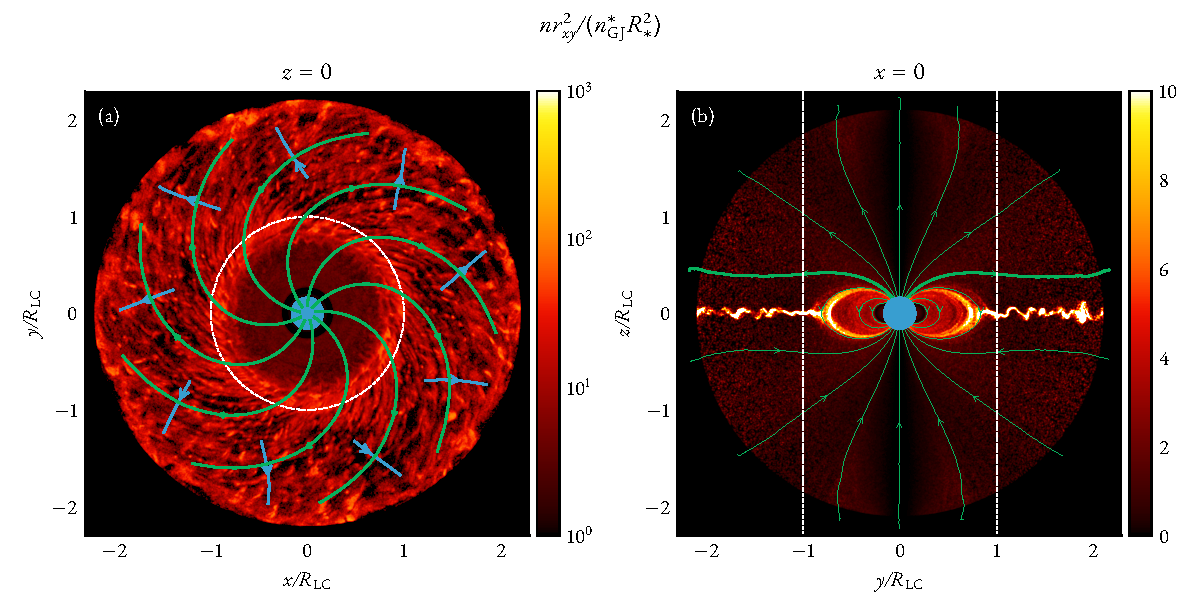
\includegraphics[width=\columnwidth]{figures/ch3-pulsar/fig2.pdf}
\caption{(a): equatorial slice of the plasma density from a simulation of an aligned rotator (\texttt{R75\_ang0}). Magnetic field lines originating at the stellar surface at about $30^\circ$ from the pole are shown with green lines. Blue arrows trace the direction of the equatorial current in the current sheet. White dashed circle indicates the light cylinder. Ripples in density are caused by the combined effect of two instabilities (tearing and kink) on the current sheet. (b): poloidal slice of the plasma from an axisymmetric simulation. As in (a), green lines show the direction of the magnetic field, while the two bold field lines correspond to the ones in panel (a). White dashed lines correspond to the position of the light cylinder. In this slice the kink-instability of the current sheet is apparent.}
\label{fig:psr-pulsarslice}
\end{figure}

\subsection*{\small\it Kinetic solution}
\label{psr:sub_kinetic_sol}

Let us closely inspect the structure of the magnetosphere in one of our simulations. For simplicity, we will consider an aligned rotator, $\chi=0^\circ$, where $R_{\rm LC} / d_e^{\rm LC} = 100$, $R_* = 75\Delta x$, and $R_{\rm LC} / R_* = 6$ (here and further we will refer to this simulation as \texttt{R75\_ang0}).\footnote{Simulations with the same basic parameters and other obliquity angles are, correspondingly, \texttt{R75\_ang20}, \texttt{R75\_ang60}, and \texttt{R75\_ang90}.} Snapshots of that simulation are shown in Figure~\ref{fig:psr-pulsarslice}. Cartesian coordinates are normalized to the $R_{\rm LC}$, and $(0, 0, 0)$ is the middle of the box, where the center of the neutron star is. Figure~\ref{fig:psr-pulsarslice}a shows the slice of the simulation in the $z=0$ plane, while Figure~\ref{fig:psr-pulsarslice}b shows the slice in the $x=0$ plane. Color indicates the plasma number density compensated by the cylindrical radius squared, $n r_{xy}^2$; its value is normalized by the corresponding GJ density at the surface of the star times the radius of the star squared, $n_{\rm GJ}^* R_*^2$. From the pictures it is evident that the total plasma density close to the current sheet exceeds the local GJ density few to ten times, which means the magnetosphere is quenched.

Projections of magnetic field lines to corresponding slices are shown with green. Thick field lines in the toroidal slice, Figure~\ref{fig:psr-pulsarslice}a, originate from the same points at the surface of the star as the thick field lines in the poloidal slice, Figure~\ref{fig:psr-pulsarslice}b. In the wind zone close to the equator ($\theta\approx \pi/2$) the structure of the magnetic field is close to that of the spinning (split-)monopole \citep{1973ApJ...180L.133M}:

\begin{equation}
\begin{split}
\label{eq:psr-bfields}
    B_{\runit}(r) =& B_{\rm LC}\left(\frac{R_{\rm LC}}{r}\right)^2,\\
    B_{\phiunit}(r) =& B_{\rm LC}\left(\frac{R_{\rm LC}}{r}\right),
\end{split}
\end{equation}
\noindent with $r$ being the distance from the center of the neutron star, and $B_{\rm LC} = B_*\left(R_*/R_{\rm LC}\right)^3$. In the closed zone the magnetic field lines are purely poloidal and their radial decay is close to $1/r^3$. 

Overdense region in the equatorial plane outside the light cylinder is the current sheet. Flapping of the current sheet in the poloidal slice, as well as the spiraling structures following the magnetic field lines in the $z=0$ slice, is the consequence of the kink instability (more on that in Section~\ref{sec:psr-dissipation}). Average directions of the local current density in the sheet are shown with blue arrows in Figure~\ref{fig:psr-pulsarslice}a. This current originates at the surface of the star near the boundary layer of the polar cap and propagates outwards along the separatrix line (the last closed field line). 

Since the current sheet is charged, there is a net poloidal electric field, $E_{\thetaunit} = B_{\phiunit}$. As a result, the pulsar radiates electromagnetic energy in the form of a radial Poynting flux: $(4\pi / c)\bm{S} = \bm{E}\times\bm{B} = E_{\thetaunit} B_{\phiunit} \runit$. This flux, integrated over a sphere that encloses the light cylinder, is the \emph{spin-down energy} of the neutron star, often denoted as $\dot{E}$ (for an aligned rotator):

\begin{equation}
\label{eq:psr-edot}
\begin{split}
    \dot{E} \equiv L_0 &= \oiint\limits_{r=R_{\rm LC}} \bm{S} \cdot d\bm{a} \\
    &= 2\pi \frac{B_*^2 R_*^3}{P}\left(\frac{R_*}{R_{\rm LC}}\right)^3.
\end{split}
\end{equation}

If there were no energy dissipation in the magnetosphere, the integral in \eqref{eq:psr-edot} would have been constant with $r$, or in other words the $L(r)=const$. However, as we will demonstrate in the upcoming section, magnetic energy is being constantly dissipated in the equatorial current sheet. This dissipation is driven by a magnetic reconnection, a microscopic process that transfers the electromagnetic Poynting flux to energized particles in the current sheet.

\section{Dissipation of spin-down energy}
\label{sec:psr-dissipation}

The structure of the magnetosphere in PIC is very similar to that in force-free. This should come as no surprise, since in our simulations the $\bm{E}_\parallel$ is perfectly screened with abundant plasma, and magnetized particles follow field lines almost everywhere. The key difference from force-free solutions is the dynamics of the equatorial current sheet. In ideal force-free the energy dissipation in the current sheet is caused purely by the numerical resistive diffusion of the magnetic field. PIC algorithm, however, enables us to ``resolve'' this dissipation at plasma kinetic scales. This allows us to self-consistently predict the efficiency of this dissipation, describe the non-linear plasma dynamics of the current sheet, and, ultimately, predict the particle distributions and emission spectra (more on that in Section~\ref{sec:psr-radiation}). 

\subsection*{\small\it Kinetic instabilities in the current sheet}

The equatorial current sheet highlighted in Figure~\ref{fig:psr-pulsarslice} is not laminar even in the case when $\chi=0^\circ$. Rather it is prone to kinetic instabilities, that develop at microscopic timescales comparable to $\omega_{{\rm p}e}^{-1}$. \emph{Kink instability} displaces the current sheet in $z$-direction, which results in flapping of the sheet as shown in poloidal slice (Figure~\ref{fig:psr-pulsarslice}b). The wave-vector of this perturbation is perpendicular to the local magnetic field and is parallel to the current density. This instability by itself does not dissipate the electromagnetic energy, and only changes the form of the otherwise laminar current sheet at microscopic plasma scales. 

More importantly, the current sheet also experiences \emph{tearing instability} due to relativistic reconnection of magnetic field lines from the upstream. As a result of this process, plasmoids are formed containing hot plasma energized in the reconnection process. In-between the plasmoids there are regions where magnetic energy dissipation happens, the \emph{x-points}.

Figure~\ref{fig:psr-pulsar3d}c shows a 3D rendering of the plasma density as well as two slices of the same quantity: one along the magnetic field lines (Figure~\ref{fig:psr-pulsar3d}a indicated with a red surface in panel \ref{fig:psr-pulsar3d}c), and the other one -- perpendicular to field lines, along the direction of the current (Figure~\ref{fig:psr-pulsar3d}b indicated with a blue surface). On panel Figure~\ref{fig:psr-pulsar3d}b one can see the flapping of the current sheet due to the kink instability. The reconnection and tearing instability, on the other hand, are better visible in Figure~\ref{fig:psr-pulsar3d}a; overdense regions in the sheet are the plasmoids, which in 3D look like dense flux tubes elongated almost radially (Figure~\ref{fig:psr-pulsar3d}c). 

\begin{figure}[htb]
\centering
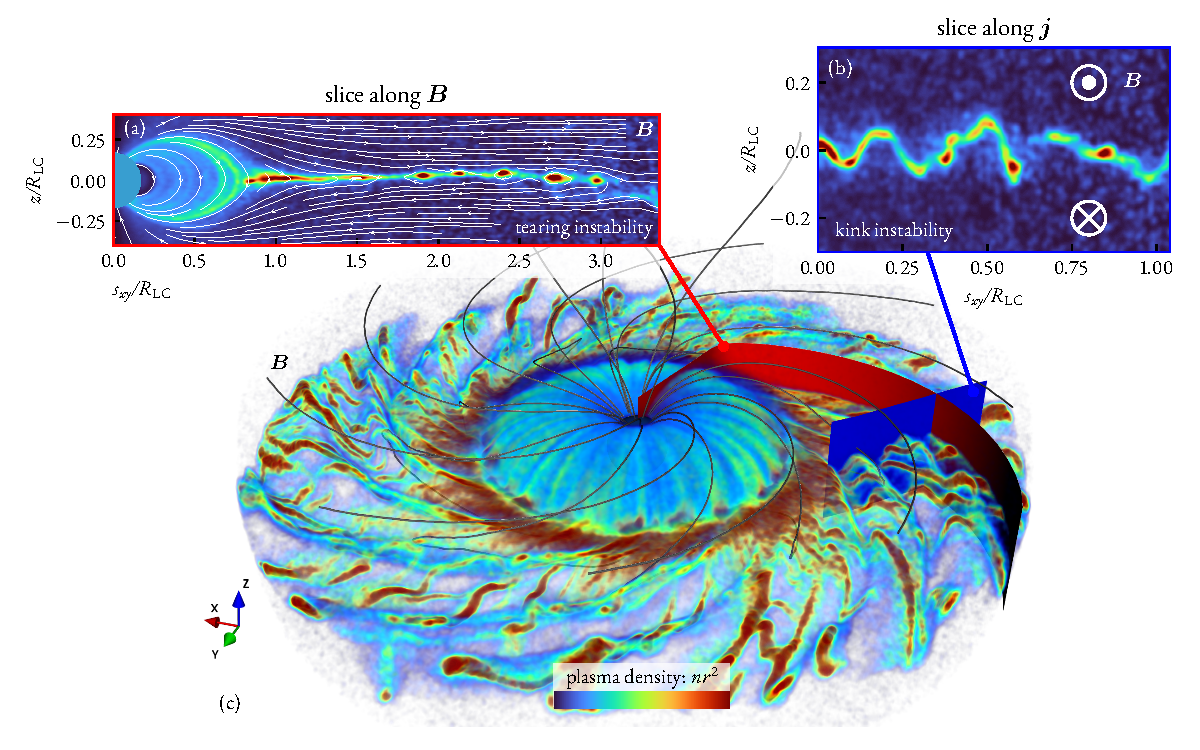
\includegraphics[width=\columnwidth,trim={10 10 10 5},clip]{figures/ch3-pulsar/fig3.pdf}
\caption{3D rendering of the plasma density (compensated by $r^2$) from a simulation of an aligned rotator (\texttt{R75\_ang0}). 3D rendering (panel c) is accompanied by the two slices (a and b, also visible in 3D as red and blue planes). One of the slices (a) is along the upstream magnetic field, while the second one (b) is along the direction of the current perpendicular to the magnetic field. Overdense elongated tubes in panel (c) are the 3D flux ropes, the plasmoids, which are produced as a result of the non-linear tearing instability. In a 2D slice (a) the dynamics of both the current sheet and the plasmoids themselves look very similar to those in localized current sheet simulations. In panel (b) kink instability is visible, which deforms the current sheet in the direction perpendicular to the direction of the tearing instability. An animated version of this plot is available with the following link: \url{https://youtu.be/-YXJ4yTlhWw}.}
\label{fig:psr-pulsar3d}
\end{figure}

In the rotating frame the dynamics of the reconnecting current sheet in slice \ref{fig:psr-pulsar3d}a is very similar to the one in a 2D Harris sheet, except for the fact that both the upstream and the current sheet are flying outwards with bulk $\Gamma\sim \mathcal{O}(1)$. In the upstream (above and below the current sheet) the plasma motion is strictly constrained by magnetic field lines. Cold plasma and opposing magnetic field lines are brought together by an $\left(\bm{E}\times\bm{B}\right)_z$ drift (shown in Figure~\ref{fig:psr-reconnection}a); the current sheet then becomes unstable and tears producing plasmoids (shown with magenta contours). The dimensionless rate of inflow is set by reconnection; this value can be directly measured for an axisymmetric pulsar (Figure~\ref{fig:psr-reconnection}a). For our simulations this value is close to
\begin{equation}
    \beta_{\rm rec} \equiv \frac{\left(\bm{E}\times\bm{B}\right)_{\rm in}}{|\bm{B}|^2} \approx 0.1\text{-}0.2.
\end{equation}

\begin{figure}[htb]
    \sidebysidecaption{0.555\linewidth}{0.42\linewidth}{
        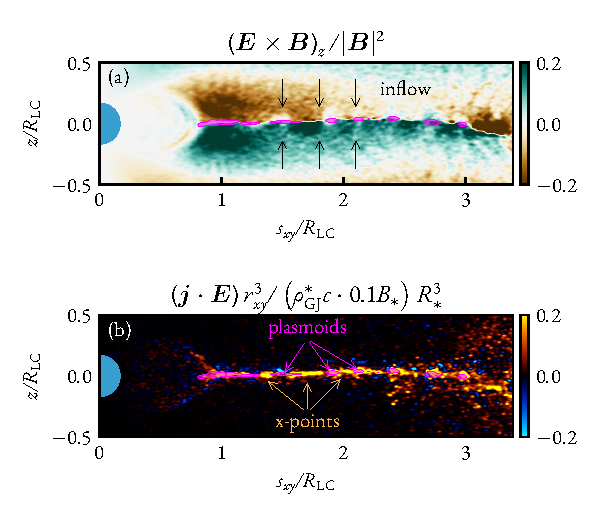
\includegraphics[width=\columnwidth,trim={10 10 10 5},clip]{figures/ch3-pulsar/fig4.pdf}
    }{
        \caption{Two panels show different quantities in the same slice as Figure~\ref{fig:psr-pulsar3d}a. (a) shows the  $\bm{E}\times\bm{B}$ inflow rate into the current sheet; this corresponds to the rate at which the reconnection of magnetic field lines occur, roughly, $\beta_{\rm rec}\sim 0.1$. In panel (b) we plot the work done by the electric field on current-carrying charges (compensated by $r_{xy}^3$). This term is responsible for the dissipation of the spin-down Poynting flux in the magnetosphere. The dissipation is mostly focused in the thin equatorial region, the current sheet. On both panels we overplot the plasmoids in magenta (they are clearly visible in Figure~\ref{fig:psr-pulsar3d}a).}
        \label{fig:psr-reconnection}
    }
\end{figure}

\subsection*{\small\it Magnetic energy dissipation via reconnection}

Reconnecting magnetic field in the current sheet generates an accelerating non-ideal electric field in the direction of the $\nabla\times \bm{B}$, same as the direction of the current in Figure~\ref{fig:psr-pulsarslice}a (in Figure~\ref{fig:psr-pulsar3d}a and Figure~\ref{fig:psr-reconnection}a,b that corresponds to the out-of-plane direction). Its magnitude is of the order of $E_{\rm rec}\sim \beta_{\rm rec}B_{\rm up}$, where $B_{\rm up}$ is the magnetic field strength in the upstream. Because of the emergence of $\bm{j}\cdot \bm{E}$ (shown in Figure~\ref{fig:psr-reconnection}b) the Poynting flux radiated by the star \eqref{eq:psr-edot} dissipates in the magnetosphere. As seen in Figure~\ref{fig:psr-reconnection}b dissipation occurs exclusively in the current sheet outside the light cylinder, where the energy of the electromagnetic field is converted into the kinetic energy of plasma through magnetic reconnection. According to Poynting's theorem:

\begin{equation}
\label{eq:psr-poynting-th}
    L(r) - L_0 \equiv \oiint\limits_{R_{\rm LC}}^r \bm{S} d\bm{a} = -\iiint \bm{j}\cdot \bm{E}d^3\bm{r}.
\end{equation}
\noindent This yields to the fact that $L(r)$ is a decaying function of radius. Figure~\ref{fig:psr-dissipation} shows the $L(r)$ from one of our simulations with $\chi=0^\circ$ computed using the flux of the Poynting vector (blue line), and the volume integral of $\bm{j}\cdot\bm{E}$ (red line). Orange band corresponds to an analytical model described in the next paragraph.

To understand the dependence of $L(r)$ it is useful to build a simple analytical model of the Poynting flux dissipation in the current sheet. For $\chi=90^\circ$ rotator this model has been studied by \cite{2020A&A...642A.204C}; here we focus on $\chi=0^\circ$. As mentioned earlier, the dissipation of Poynting flux is caused by the work done by the reconnection electric field, $\bm{j}\cdot\bm{E}$, as described by \eqref{eq:psr-poynting-th}. The strength of the electric field generated due to magnetic reconnection at a given distance $r$ from the star is $E_{\rm rec}(r)\sim\beta_{\rm rec} B_{\rm up}(r)$. Here the reconnecting magnetic field is a combination of poloidal and toroidal components from \eqref{eq:psr-bfields} $B_{\rm up}(r) =\sqrt{B_\runit^2 + B_\phiunit^2}$.\footnote{This is the main difference with the $\chi=90^\circ$ case, where only toroidal component of the magnetic field is reconnecting.} Since $(4\pi/c)\bm{j}=\nabla\times\bm{B}$, current, generated during the reconnection can be estimated as $j\sim c B_{\rm up} / (2\pi \delta_{\rm cs})$, where $\delta_{\rm cs}$ is the characteristic width of the current sheet. Thus, the volume integral in \eqref{eq:psr-poynting-th} reduces to:

\begin{equation}
\label{eq:psr-luminosity-int}
    L(r) - L_0 = -\int\limits_{R_{\rm LC}}^r dr\int\limits_0^{2\pi}d\phi \int\limits_0^\pi d\theta r^2\sin{\theta} \left(\frac{\beta_{\rm rec} c}{2\pi \delta_{\rm cs}}B_{\rm up}^2\right).
\end{equation}
\noindent Integral over the azimuthal angle $\phi$ is trivial because of the axisymmetry. Integral over the polar angle, $\theta$, at each $r$ is accumulated in a small region near the equator ($\theta=\pi/2$) of angular size $\Delta \theta\sim \delta_{\rm cs}/r$ (which is the current sheet highlighted in Figure~\ref{fig:psr-reconnection}b). Integrating \eqref{eq:psr-luminosity-int} using expressions for the fields from \eqref{eq:psr-bfields} then yields

\begin{equation}
\label{eq:psr-luminosity}
    \frac{L(r)}{L_0} = 1 - \beta_{\rm rec}\left(\ln{\frac{r}{R_{\rm LC}}}
    +\frac{1}{2}\left(1 -\left[\frac{r}{R_{\rm LC}}\right]^{-2}\right)\right).
\end{equation}

\noindent The logarithmic term in this relation corresponds to the dissipation of the toroidal field, $B_\phiunit$, while the second term corresponds to the dissipation of poloidal field, $B_{\runit}$. At large distances, $r\gg R_{\rm LC}$ the first term prevails, as the field is almost purely toroidal. However, for the short region, $R_{\rm LC}<r<2R_{\rm LC}$, considered in Figure~\ref{fig:psr-dissipation} contributions from both terms are important. Orange band in Figure~\ref{fig:psr-dissipation} corresponds to \eqref{eq:psr-luminosity} with $\beta_{\rm rec}$ varying from $0.09$ to $0.12$ (this number can be directly measured from Figure~\ref{fig:psr-reconnection}a). For other values of $\chi$ our results are consistent with earlier works (PIC: \citealt{2015ApJ...801L..19P}, and MHD: \citealt{2013MNRAS.435L...1T}). Namely, the spin-down luminosity near the light cylinder $\oint \bm{S}d\bm{a}\approx L_0(1 + \sin^2{\chi})$, and for larger values of $\chi$ we see inhibited dissipation in the current sheet, as the jump of the magnetic field across the current sheet is diminished for larger $\chi$.

\begin{figure}[htb]
    \sidebysidecaption{0.555\linewidth}{0.42\linewidth}{
        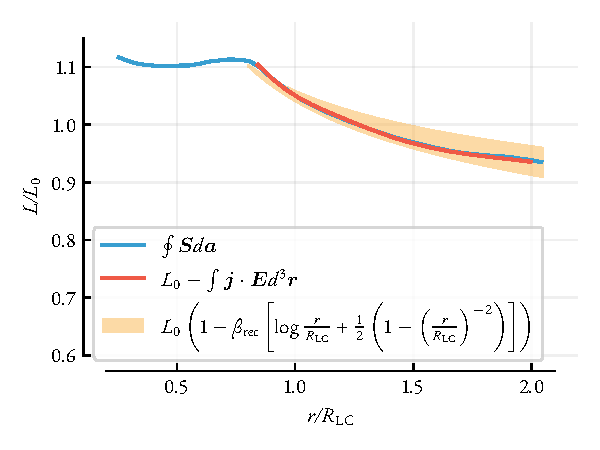
\includegraphics[width=\columnwidth,trim={10 10 10 5},clip]{figures/ch3-pulsar/fig5.pdf}
    }{
    \caption{Dissipation of the spin-down Poynting flux in the outer magnetosphere from a simulation of an aligned rotator. The blue line is the direct measurement of the Poynting flux vs $r$. The red line shows the work done by the electric field on charges, $\bm{j}\cdot\bm{E}$, which, according to Poynting's theorem, accounts for the dissipation of the Poynting flux. Orange band is the theoretical fit \eqref{eq:psr-luminosity} with $\beta_{\rm rec}\approx 0.09\textrm{-}0.12$. $L_0$ is computed from \eqref{eq:psr-edot}. A slight increase of $L$ with respect to $L_0$ in the inner magnetosphere is due to the fact that the Y-point in our simulation is slightly shifted inside w.r.t. the $r/R_{\rm LC} = 1$; this leads to slightly more open field lines and thus more Poynting flux.}
    \label{fig:psr-dissipation}
    }
\end{figure}

Dissipated energy of the magnetic field during the reconnection in the current sheet is deposited into plasma particles. In the next section we focus on particle energization in the current sheet and its consequences on the observed high-energy emission in $\gamma$-ray pulsars.

\section{Particle acceleration and $\gamma$-ray emission}
\label{sec:psr-radiation}
Relativistic magnetic reconnection is known to produce non-thermal particle population \citep{2014ApJ...783L..21S}; reconnection in the current sheets of neutron star magnetospheres is no exception. These energized particles are believed to radiate via synchrotron mechanism, producing the pulsed high-energy emission observed in $\gamma$-ray pulsars \citep{2016MNRAS.457.2401C,PSAS18}.

\subsection*{\small\it Efficiency of magnetic reconnection and synchrotron cooling}

Main parameter that determines the efficiency of particle acceleration during reconnection is \emph{the magnetization} of the upstream (unreconnected) plasma, $\sigma$. For the given background magnetic field, $B$, and the number density of inflowing plasma, $n$, this dimensionless parameter is equal to twice the ratio of the magnetic energy density and the rest mass energy density of plasma. Or equivalently, it is equal to the square of the ratio of gyrofrequency to plasma frequency (for cold particles with $\beta\gamma\approx 1$):
\begin{equation}
    \sigma \equiv \frac{B^2/4\pi}{n m_e c^2} = \left(\frac{\omega_{B}}{\omega_{{\rm p}e}}\right)^2.
\end{equation}
\noindent This parameter, which is $\gg 1$ in case of relativistic reconnection, determines the characteristic maximum energy to which particles can be accelerated in the single x-point (or x-line in 3D, see Figure~\ref{fig:psr-reconnection}b). If secondary reacceleration is prohibited, i.e. if particles leave the system as soon as they get accelerated in a single x-point, their non-thermal distribution function extends at most to energies of a few times $\sigma m_e c^2$. Energized particles, however, may either then reenter the current sheet or become trapped in plasmoids and get accelerated again via secondary processes to even higher energies \citep{2018MNRAS.481.5687P,2021ApJ...912...48H}. However, as we demonstrate below, in pulsar magnetospheres with realistic parameters this is almost impossible due to the chaotic nature of the current sheet and the synchrotron losses. 

Synchrotron cooling may slow down particles at timescales comparable to the acceleration timescale in the current sheet, affecting the emerging non-thermal particle distribution. The efficiency of cooling is determined by the strength of the magnetic field. This can be conveniently quantified with a dimensionless number, $\gamma_{\rm rad}$, easily transferable to PIC simulations. This number corresponds to the Lorentz factor of particles for which the synchrotron cooling timescale in a given background magnetic field $B$ is comparable to the acceleration timescale due to reconnection (acceleration in an electric field of strength $E\sim \beta_{\rm rec}B$):

\begin{equation}
    |e|\beta_{\rm rec}B c = \frac{2}{3}r_e^2 c B^2 \gamma_{\rm rad}^2,
\end{equation}
\noindent where $r_e=e^2/m_e c^2$ is the classical radius of the electron.\footnote{In terms of PIC simulations, defining dimensionless $\gamma_{\rm rad}$ is equivalent to upscaling the classical electron radius, $r_e$, which would otherwise be severely underresolved. Also note, that in this rough definition the magnetic field is considered to be exactly perpendicular to the motion of a particle. In our simulations, as well as in reality, particles flying at small pitch angles w.r.t. the magnetic field will be cooled less efficiently. Thus, $\gamma_{\rm rad}$ can be thought of as just a proxy for the average cooling efficiency for a population of isotropically distributed particles.} Particles with $\gamma \gg \gamma_{\rm rad}$ will lose their energies as soon as they are exposed to a perpendicular magnetic field component much faster than they are able to accelerate, while the opposite is true for particles with $\gamma \ll \gamma_{\rm rad}$. 

Guided by the $\sigma$-limit of the acceleration during magnetic reconnection, we will call the cooling \emph{strong} when $\gamma_{\rm rad} < \sigma$, while the opposite case will be referred to as the \emph{weak cooling} regime. Naively, one could think that in the reconnection process with strong cooling particles cannot gain energies higher than $\gamma_{\rm rad} m_e c^2$, as for these particles the cooling becomes faster than the acceleration. However, this is not necessarily true, as the acceleration takes place in the region of the current sheet where there is virtually no cooling (the magnetic field is zero in the x-points; we show this below, and this has also been demonstrated in 2D simulations by \citealt{2019ApJ...877...53H}). On the other hand, in the strong cooling regime once particles leave the accelerating regions (either back to the upstream or into plasmoids), they very quickly lose their energies without a chance to get reaccelerated again to energies larger than a few $\sigma m_e c^2$. This results in qualitatively different radiation spectra in two different cooling regimes. While cutoff energies of photons are still comparable, as plasma particles are still able to accelerate to $\gamma\sim \sigma$ in x-points, the peak of the radiation is shifted to lower energies in the strong cooling regime ($\gamma_{\rm rad}/\sigma \ll 1$), because particles are unable to retain energies $\gamma>\gamma_{\rm rad}$ for longer times.

The value of $\gamma_{\rm rad}$ (close to the light cylinder) only depends on the magnetic field strength:
\begin{equation}
    \gamma_{\rm rad}^{\rm LC}\approx 10^5\left(\frac{B_{\rm LC}}{10^5~\text{G}}\right)^{-1/2},
\end{equation}
\noindent which we know rather reliably for pulsars by extrapolating the magnetic field strength at the surface. The magnetization, $\sigma_{\rm LC}$, on the other hand, depends on plasma density near the light cylinder which is generally unknown. However, we can estimate that approximately, by assuming that the cutoff frequency of the $\gamma$-ray photons corresponds to the synchrotron peak energy for the highest-energy particles with $E\sim 10 \sigma_{\rm LC} m_e c^2$:
\begin{equation}
    \hbar \omega_B^{\rm LC} (10\sigma_{\rm LC})^2 \approx E_{\rm cut}.
\end{equation}
\noindent This provides a rough empirical estimate for $\sigma_{\rm LC}$. For the population of young pulsars $\sigma$ value is between $10^5$ and $10^6$, and the ratio $\gamma_{\rm rad}^{\rm LC}/\sigma_{\rm LC}$ varies between $0.5\text{-}2$ (for the Crab the value is $2$). We also note that the pulsars with stronger synchrotron cooling at the light cylinder typically have $\gamma$-ray spectra shifted to lower energies ($<0.1$ MeV).

In our simulations we keep $\sigma\gg 1$ in the outer magnetosphere (to ensure the reconnection is in the ultra-relativistic regime), and vary the ratio $\gamma_{\rm rad}/\sigma$. Following the discussion earlier, this ratio determines the relative importance of the effects of synchrotron cooling on reconnection dynamics, and, as we demonstrate later, results in qualitatively different high-energy radiation spectra.

\subsection*{\small\it Particle distributions and photon spectra in the radiatively cooled magnetosphere}

For the simulation \texttt{R75\_ang0} magnetization parameter in the upstream, shown in Figure~\ref{fig:psr-sigma}, is close to $\sigma_{\rm LC}\sim 10^3$ in the upstream (as shown with the linear plot on the right) and drops to zero inside the current sheet, where the magnetic field reconnects. This means that the characteristic energies to which particles can get accelerated in the current sheet is comparable to $\sigma m_e c^2$ (as will be demonstrated shortly).

\begin{figure}[htb]
    \sidebysidecaption{0.555\linewidth}{0.42\linewidth}{

        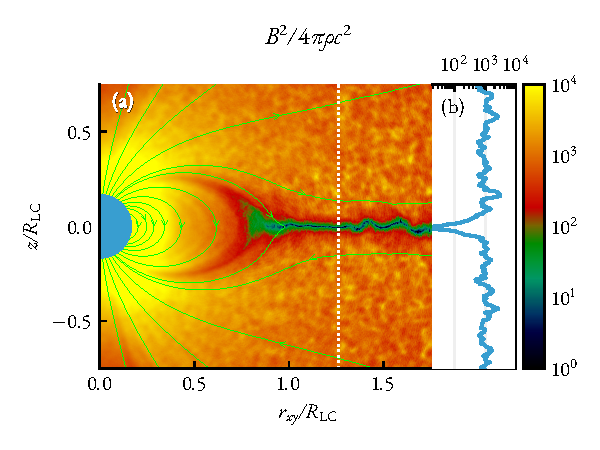
\includegraphics[width=\columnwidth,trim={10 10 10 5},clip]{figures/ch3-pulsar/fig6.pdf}
    }{
        \caption{(a): plasma magnetization parameter, $\sigma$, in a poloidal slice of the simulation \texttt{R75\_ang0}. 1D slice of the $\sigma$ across the current sheet is shown in panel (b). Magnetization of the upstream is close to $10^3$, while the background plasma density $n\sim \text{few}\cdot n_{\rm GJ}^*(R_*/r)^2$. Magnetic field lines are shown with green in panel (a).}
        \label{fig:psr-sigma}
    }
\end{figure}

Let us consider distribution functions for $e^\pm$ in different regions of our simulation \texttt{R75\_ang0}, as shown in Figure~\ref{fig:psr-spatial_spectra}. On a poloidal slice in panel \ref{fig:psr-spatial_spectra}a we show the bulk Lorentz factor of the plasma, $\Gamma = \sqrt{1 + \bm{U}^2/c^2}$, which is computed using the bulk four-velocity, $\bm{U} = \int \bm{u}f(\bm{u})d^3\bm{r}$. Panels \ref{fig:psr-spatial_spectra}b, \ref{fig:psr-spatial_spectra}c, and \ref{fig:psr-spatial_spectra}d show distribution functions of the electrons and positrons in three different regions: in the separatrix (last closed field line), in the current sheet, and in the upstream correspondingly. \emph{Upstream} plasma is relatively cold; electrons and positron are carried outwards almost radially via an $\bm{E}\times\bm{B}$ drift, gaining characteristic bulk Lorentz factors of $\Gamma \sim 10$ on scales of our simulation (Figure~\ref{fig:psr-spatial_spectra}d). On \emph{the separatrix} (Figure~\ref{fig:psr-spatial_spectra}b) both electrons and positrons from the surface are marginally accelerated by an unscreened electric field, gaining energies close to $\langle\gamma \rangle\sim 10\text{-}100$. This region also hosts hot electrons returning from the current layer, which is evident from the excess of electrons at Lorentz factors of a few $10^2$ shown in Figure~\ref{fig:psr-spatial_spectra}b. 

These two regions, the upstream and the separatrix, act as an ``intake'' and an ``exhaust'' for \emph{the current sheet}. It is important to note, that particles in these regions are generally exposed to a substantial orthogonal magnetic field component. This means that high-energy particles from the current sheet cannot exist there for timescales longer than the short cooling time. Thus, the main role in shaping the observed $\gamma$-ray emission is played by the current sheet, where constant release of magnetic energy sustainably accelerates particles in x-lines, where the magnetic field strength is zero (the cooling is non-existent).

In the current sheet (Figure~\ref{fig:psr-spatial_spectra}c) we see a substantial non-thermal particle population, extending to $\gamma\sim \sigma\sim 500\text{-}1000$. The bulk motion of the current sheet, on the other hand, has a Lorentz factor of $\Gamma\sim 10\text{-}100$, consistent with characteristic velocities of relativistic flows along the current sheet during the reconnection, $\Gamma\sim \sqrt{\sigma}$.\footnote{Slight enhancement is due to the fact that there is a bulk $\bm{E}\times\bm{B}$ outflow of the current sheet, similar to the wind in the upstream.} Notice also, that the distributions of electrons and positrons are slightly different: positrons extend to slightly higher energies. This is due to the fact that the electric field generated during reconnection ``pushes'' the electrons opposite to the global $\bm{E}\times\bm{B}$ drift, which is charge-invariant and directed radially outward (in Figure~\ref{fig:psr-pulsar3d}a the reconnection electric field is pointing in the out-of-plane direction). This difference in the electrons and positrons has been observed in earlier simulations \citep[see, e.g.,][]{PSAS18}; however, it almost vanishes for large obliquity angles, $\chi$, which we also see in our simulations.

\begin{figure}[htb]
\centering
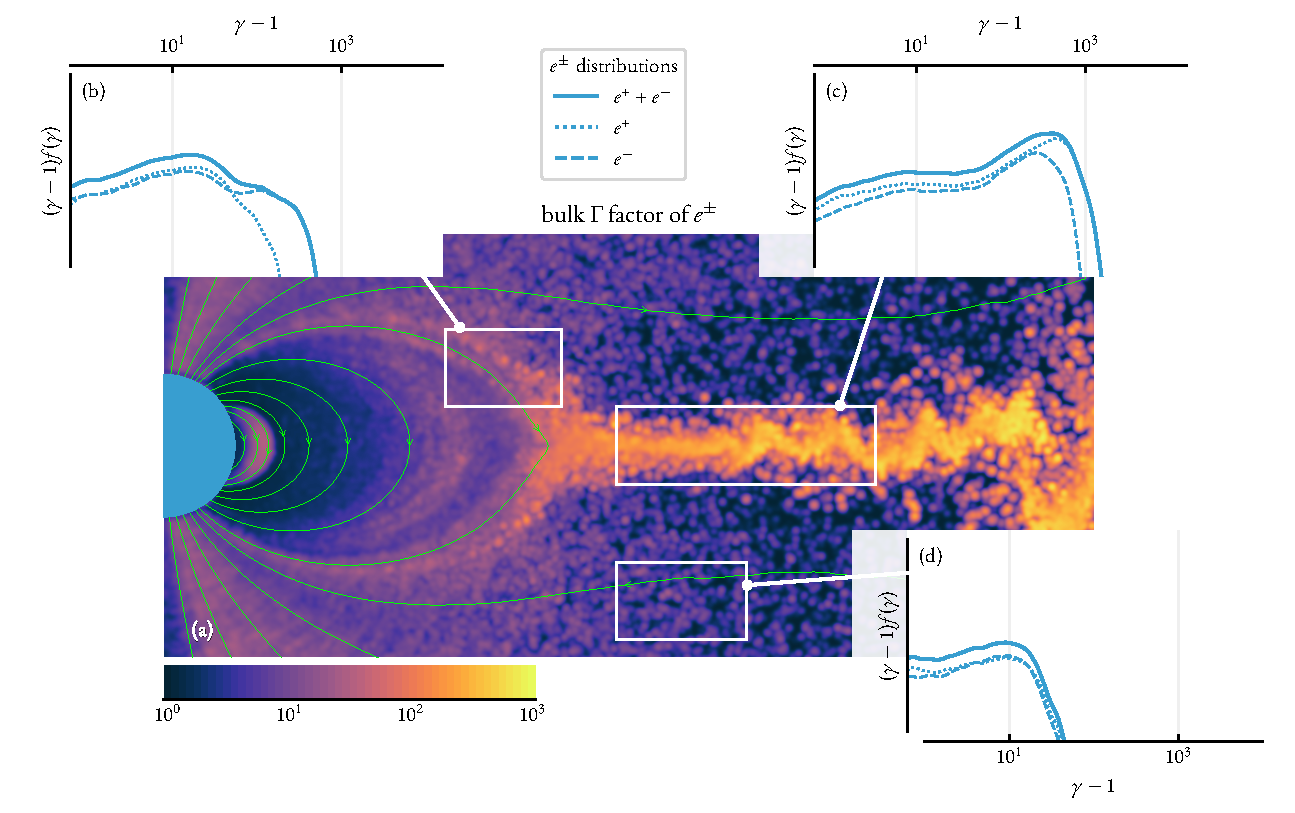
\includegraphics[width=\columnwidth,trim={10 0 10 5},clip]{figures/ch3-pulsar/fig7.pdf}
\caption{Distribution functions of electrons and positrons measured in different locations of our simulation. Bulk Lorentz factor is shown in panel (a). Panels (b), (c), and (d) show distribution functions in the separatrix, the current layer and the upstream, correspondingly. Plasma in the upstream is typically cold with a bulk outflow Lorentz factor of a few. As expected, the highest energy particles are produced in the current layer where magnetic reconnection occurs.}
\label{fig:psr-spatial_spectra}
\end{figure}

We now study the effects of different cooling regimes, i.e., different values of $\gamma_{\rm rad}/\sigma$, on both the global kinetic solution, as well as the particle and the photon spectra. Since an aligned pulsar with $\chi=0^\circ$ is pathological as it does not produce any modulated emission, most of the $\gamma$-ray pulsars are thought to have inclination angles $0<\chi<90^\circ$. We thus closely inspect two simulation setups with $\chi=20^\circ$ and $\chi=60^\circ$ (these simulations will be referred to as \texttt{R75\_ang20}, and \texttt{R75\_ang60}; all the other parameters except for the inclination angle are the same as in \texttt{R75\_ang0}). In a series of runs we keep $\sigma_{\rm LC}\approx 500\text{-}1000$ and vary $\gamma_{\rm rad}^{\rm LC}$ to capture the following regimes: $\gamma_{\rm rad}^{\rm LC}/\sigma_{\rm LC}=1/15,~1/3,~2,\infty$ (where $\gamma_{\rm rad}=\infty$ corresponds to simulation without synchrotron cooling; for a future reference, these simulations we denote as \texttt{R75\_ang20\_gr1o15}, \texttt{R75\_ang60\_gr1o15}, ..., \texttt{R75\_ang60\_grINF}).

\begin{figure}[htb]
    \sidebysidecaption{0.555\linewidth}{0.42\linewidth}{
        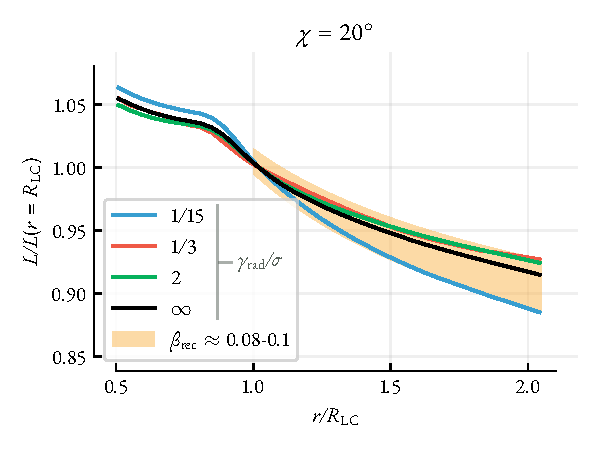
\includegraphics[width=\columnwidth,trim={10 0 10 5},clip]{figures/ch3-pulsar/fig10.pdf}
    }{
        \caption{Poynting flux dissipation as a function radius, $L(r)$, for different cooling regimes in \texttt{R75\_ang20}. Reconnection rate and, thus, the dissipation is only marginally affected by the strength of synchrotron cooling.}
        \label{fig:psr-rad-dissipation}
    }
\end{figure}

We find that the general structure of the current sheet is largely unaffected by the strength of synchrotron cooling. In the most extreme case $\gamma_{\rm rad}^{\rm LC}/\sigma_{\rm LC}=1/15$ plasmoids become slightly more compressed as radiation reaction suppresses the perpendicular plasma pressure which holds plasmoids in equilibrium counteracting the $\bm{j}\times\bm{B}$ force. Nevertheless, the rate of magnetic reconnection and, as a result, the Poynting-flux dissipation curves, $L(r)$, are only marginally affected as seen in Figure~\ref{fig:psr-rad-dissipation} for $\chi=20^\circ$. 

Particle distribution functions in the current sheet are also very similar in all of the cooling regimes, as shown in Figures~\ref{fig:psr-spec20}a and \ref{fig:psr-spec60}a. In all of the studied cases particles in the current are able to accelerate to $\sim\sigma_{\rm LC}$ in x-points, forming a power law of $f\propto \gamma^{-1}$ (for $\chi=60^\circ$ the spectrum is slightly steeper). Only in the most strongly cooled simulation we see that the cutoff of particle distribution is slightly shifted towards lower energies. This is most likely an effect of comparably small scale separation in our simulations, which will most likely be unnoticable for realistic systems. Since x-lines in 3D have finite extent, in a single encounter particles are unable to tap the full potential drop across it. Thus, typically, particles will need several encounters to be accelerated to highest energies. In the strongest cooling case, however, as soon as particles leave the x-point, they are cooled almost instantly either in the upstream or in plasmoids. These conclusions are consistent with 2D local simulations of radiative magnetic reconnection by \cite{2019ApJ...877...53H}. In weakly cooled simulations above $\gamma>\sigma_{\rm LC}$ we see a smooth transition to $\gamma^{-2.5}\text{-}\gamma^{-3}$ and, eventually, to an almost exponential cutoff. We speculate that this transition, almost absent in simulations with strong cooling, might be indicative that particles are also experiencing brief secondary acceleration inside the compressing plasmoids as described by \cite{2018MNRAS.481.5687P,2021ApJ...912...48H}.

In Figures \ref{fig:psr-spec20}b and \ref{fig:psr-spec60}b we show spectra of the emitted synchrotron photons for both $\chi=20^\circ$ and $\chi=60^\circ$ simulations at different cooling regimes. In all cases we see a recurring pattern in photon spectra: a rise $\nu F_\nu\propto \nu$, a transition with a peak and a decay at higher energies. Power-law index for the distribution of photons is roughly consistent with the power-law index for the distribution of particles, i.e., $f\propto \gamma^{-p}$ leads to $\nu F_\nu \propto \nu^{-(p-3)/2}$. We see a shift of the emission peak towards lower energies for simulations with stronger cooling. Also note, that we do not observe significant intermittency at higher energies for the strong cooling simulation as predicted by \cite{2019ApJ...877...53H}. This is most likely due to a much worse scale separation, and the overall complexity in the structure of the current sheet, as compared to 2D simulations (in 2D this high energy intermittency was primarily caused by plasmoid merger events).

\begin{figure}[htb]
\centering
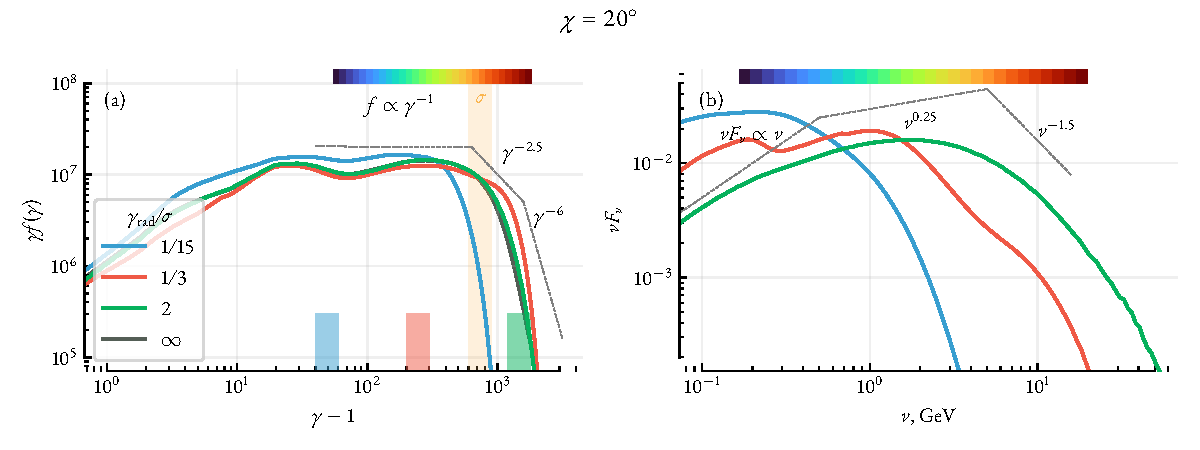
\includegraphics[width=\columnwidth,trim={10 0 10 5},clip]{figures/ch3-pulsar/fig9_a.pdf}
\caption{(a) particle and (b) photon spectra for the \texttt{R75\_ang20} simulation in different synchrotron cooling regimes. Effective $\sigma$ at the light cylinder is marked with a yellow stripe. Three smaller bars indicate the effective $\gamma_{\rm rad}$. Three power-law fits of $f\propto \gamma^{-p}$ in panel (a) translate to power-laws in photon spectra $\nu F_\nu \propto \nu^{-(p-3)/2}$. Colorbar at the top of both panels puts particle energies into correspondence with synchrotron peak energies, $\nu \propto \gamma^2 B_{\rm LC}$. While particle spectra look almost identical (except for the strongest cooled case), peaks of photons are shifted to smaller energies for smaller $\gamma_{\rm rad}/\sigma$. Only particles in the current layer are accounted for.}
\label{fig:psr-spec20}
\end{figure}

\begin{figure}[htb]
\centering
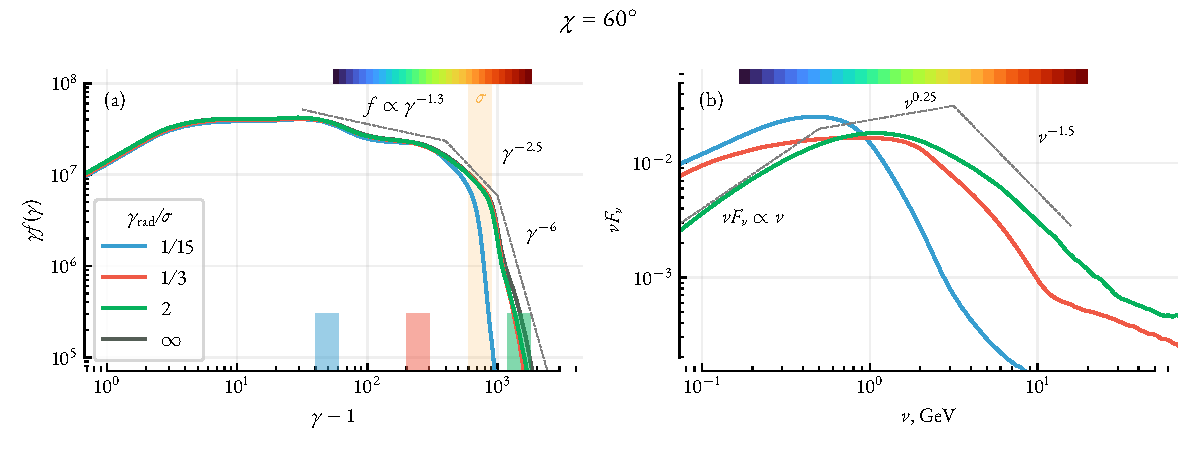
\includegraphics[width=\columnwidth,trim={10 0 10 5},clip]{figures/ch3-pulsar/fig9_b.pdf}
\caption{Same as in Figure~\ref{fig:psr-spec20} but for simulation \texttt{R75\_ang60}. Particle distributions are still largely unaffected by cooling, while the peaks of photon spectra are shifted towards lower energies for stronger cooling simulations.}
\label{fig:psr-spec60}
\end{figure}

\section{Discussion \& summary}

In this work we demonstrated the result from 3D PIC simulations of the neutron star magnetospheres with the synchrotron radiation reaction force included. Our primary focus was the energy dissipation and the plasma dynamics in the reconnecting current sheet. To be able to properly capture the kinetic physics, governing the energy extraction in the current layer we push the separation of macro-to-micro scales in our simulations to $\sim 200$, which allows to self-consistently model the hierarchical chain of plasmoids in the saturated tearing unstable regime. 

We show that the rate of inflow to reconnecting current sheet, which is controlled by plasma-kinetics at scales of microscopic x-lines, determines the dissipation rate in the entire magnetosphere. This puts a stringent constraint on how much energy can be dissipated in the current layer (and, ultimately, radiated) within a few light cylinders. From simulations we find that this dissipation rate is almost insensitive to both the bulk motion of the background unreconnected plasma, and the radiation efficiency.

We confirm that the particle distribution is almost unaffected by synchrotron cooling, with particles in the current sheet forming a hard power-law spectrum with steep cutoff at energies of $\sim \sigma_{\rm LC}m_e c^2$. Photon spectra, on the other hand, are largely different, with the stronger cooling simulations resulting in peaks shifted towards lower energies. 

These results are partly consistent with the observations by \emph{Fermi} satellite. However, we note an important difference: observations show that the pulsars with $\gamma$-ray peaks at lower energies have typically wider spectra resulting in almost constant value for the cutoff energy, $E_{\rm cut}$. This has also been confirmed in 2D localized simulations \citep{2019ApJ...877...53H}, where a wide spectrum with a slow $\nu F_\nu\propto \nu^{-1/2}$ decay was observed for the cases with strongest synchrotron cooling. This high-energy tail was mostly accumulated in the intermittent events of large plasmoid mergers, abundant in 2D simulations. In our 3D simulations, however, the limited scale separation does not allow to capture many of these events.
%% paper # 1
%%\begin{savequote}[75mm]
%Nulla facilisi. In vel sem. Morbi id urna in diam dignissim feugiat. Proin molestie tortor eu velit. Aliquam erat volutpat. Nullam ultrices, diam tempus vulputate egestas, eros pede varius leo.
%\qauthor{Quoteauthor Lastname}
%\end{savequote}

\newcommand{\linkVidOne}{https://youtu.be/VhwXzci_bY8} % large plasmoid
\newcommand{\linkVidTwo}{https://youtu.be/Mu_VYtADbnc} % weak cooling
\newcommand{\linkVidThree}{https://youtu.be/QY_Bpjr1p2Q} % strong cooling

\chapter{{\it Rhapsody}: pair-production and high-energy emission in pulsars}
\label{ch:pairproduction}

\epigraph{In collaboration with A.~Philippov, and A.~Spitkovsky}

One of the key observational characteristics of $\gamma$-ray pulsars is a hard power law spectrum (with a typical photon index $\Gamma\sim 1\text{-}2$) extending to cutoff energies of a few GeV \citep{2013ApJS..208...17A}. While pulsed radio emission is generated in the inner magnetosphere close to the neutron star surface, gamma radiation usually arrives in different rotational phases and based on its light curve properties is thought to be produced mainly in the outer magnetosphere close to the Y-point (see, e.g., \citealt{2010ApJ...715.1282B, 2010MNRAS.404..767C, 2015ApJ...811...63H}). Reconnection in the current layer beyond the Y-point just outside the light cylinder is a plausible mechanism of non-thermal particle acceleration that can later form the observed spectrum via synchrotron radiation \citep{1990ApJ...349..538C, 1996A&A...311..172L, 2012MNRAS.424.2023P, 2016MNRAS.457.2401C, PSAS18}. \par

\begin{figure}[htb]
    \sidebysidecaption{0.555\linewidth}{0.42\linewidth}{
        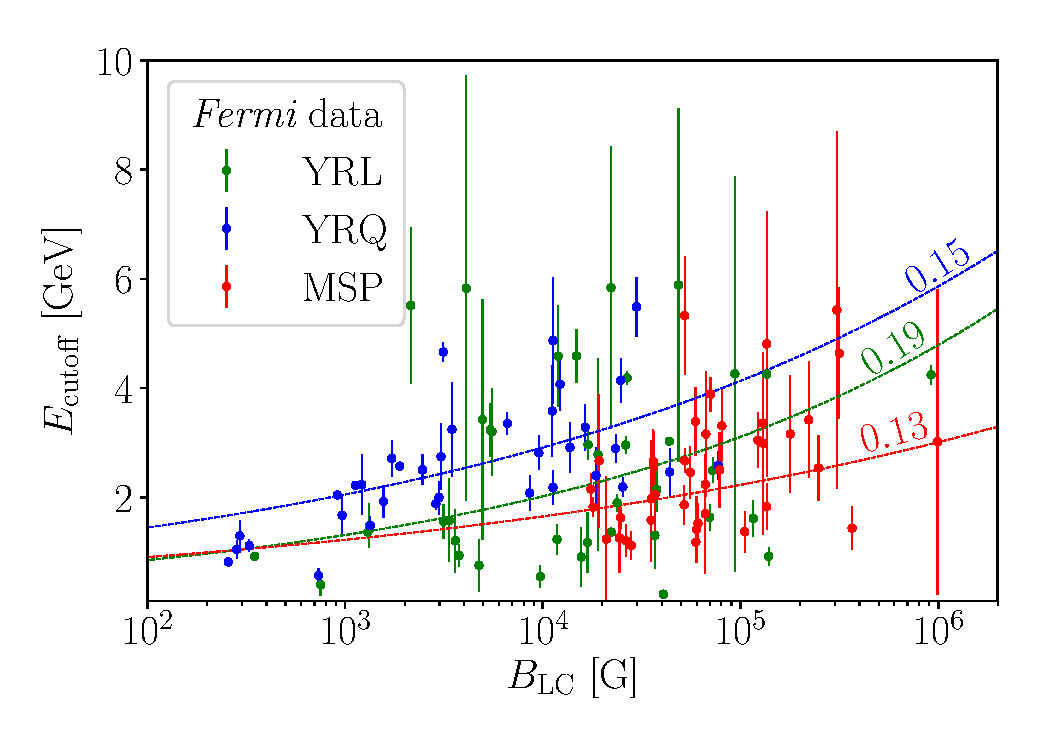
\includegraphics[width=\textwidth]{figures/ch4-pairproduction/fig1.pdf}
    }{
        \caption{Data from {\it Fermi Observatory} observations of the cutoff energy of photon spectra plotted against the estimated light cylinder magnetic fields for young radio-loud, young radio-quiet, and millisecond pulsars. The dashed lines are the best fit power laws, and the corresponding numbers are the power-law photon indices. Data taken from  \href{https://fermi.gsfc.nasa.gov/ssc/data/access/lat/2nd_PSR_catalog/}{LAT Second Catalog of Gamma-ray Pulsars} (direct link: \url{https://fermi.gsfc.nasa.gov/ssc/data/access/lat/2nd_PSR_catalog/}).}
        \label{fig:pairprod-fermi_data}
    }
\end{figure}

However, while the light curves and spectral shapes of pulsar $\gamma$-ray emission can be naturally explained with the current sheet emission, there is a disagreement between the observations and the predictions of spectral cutoff of this model. The high energy spectral cutoff in pulsars, as measured by the {\it Fermi Observatory}, depends weakly on the magnetic field at the light cylinder, $B_{\rm LC}$. As shown in Figure~\ref{fig:pairprod-fermi_data}, for a wide range of $B_{\rm LC}=10^3\text{-}10^6$ G the cutoff energy varies from $1$ to around $6$ GeV \citep{2013ApJS..208...17A}. On the other hand, the model that incorporates reconnection predicts a stronger dependence. In relativistic reconnection the magnetic energy that can be deposited into particle kinetic energy is controlled by the magnetization parameter at the light cylinder, $\sigma_{\rm LC}$, defined as the ratio of the magnetic energy to plasma enthalpy. For the cold plasma this parameter is equal to:
\begin{equation}\label{eq:pairprod-sigma_def}
    \sigma_{\rm LC}\approx \frac{B_{\rm LC}^2/4\pi}{n_{\rm LC}m_e c^2},
\end{equation}
where $B_{\rm LC}$ and $n_{\rm LC}$ are the magnetic field and the plasma density near the light cylinder. In particular, in a strongly magnetized plasma, $\sigma_{\rm LC}\gg 1$, the particle spectrum cutoff does not typically exceed few times $\sigma_{\rm LC}$ \citep{2014ApJ...783L..21S, 2016ApJ...816L...8W}. Note here, that there are mechanisms that can increase this cutoff to much higher energies in the uncooled reconnection \citep{2018arXiv180800966P}. We will discuss later why this is not possible when strong synchrotron cooling is present.

The plasma loading along the separatrix to the light cylinder and outer magnetosphere is set by the multiplicity of the primary cascade near the polar cap, $\kappa\sim 10^4$, \citep{1982ApJ...252..337D,2013MNRAS.429...20T,2018arXiv180308924T} and the local Goldreich-Julian density, $n_{\rm GJ}\approx\Omega B_{\rm LC}/2\pi c e$, i.e., $n_{\rm LC}\approx \kappa n_{\rm GJ}$. The multiplicity of primary cascade, $\kappa$, is roughly insensitive to the magnetic field strength. This means that the plasma density scales linearly with the magnetic field at the light cylinder, and thus from formula~(\ref{eq:pairprod-sigma_def}) the maximum particle energy, $\gamma_{\rm max}\sim \sigma_{\rm LC}$, also scales linearly with $B_{\rm LC}$. If these particles radiate synchrotron photons which form the observed $\gamma$-ray emission, the cutoff energy of photon spectrum, $E_{\rm cutoff}$, will correspond to the maximum energy of particle spectrum set by $\sigma_{\rm LC}$. This will lead to a strong dependence of the cutoff energy on the background magnetic field: $E_{\rm cutoff}\propto \gamma_{\rm max}^2 B_{\rm LC}\propto B_{\rm LC}^3P^2$, where $P$ is the period of the pulsar. Periods of $\gamma$-ray emitting normal pulsars vary within less than a decade; same is true for $\gamma$-ray emitting millisecond pulsars. For simplicity, we will ignore the dependence on periods in our further discussion. This discrepancy with the observed weak dependency suggests that there must be a self-regulating source of additional mass loading of the current layer that effectively decreases the magnetization and suppresses the particle acceleration for higher magnetic fields.

In the region close to the current layer the number density of high energy synchrotron photons is sufficiently high for two-photon pair production to be efficient. This process has previously been studied in the context of outer gap acceleration models \citep{1996A&AS..120C..49A, 2010ApJ...715.1318T}. As was shown by \cite{1996A&A...311..172L} for the reconnection-powered acceleration occurring in the equatorial current sheet, this pair creation process can significantly increase the plasma population with multiplicities of secondary pairs up to several thousand ($\sim 3000$ for Crab). On the other hand, thermal keV radiation from the neutron star surface is insufficiently luminous to interact with high energy GeV photons and significantly contribute to pair production. Thus, the main effect is due to high energy (keV to GeV) synchrotron photons emitted locally in the sheet interacting with each other in the current layer near the Y-point.

Since plasma loading of the reconnection layer affects the rate of reconnection and its acceleration properties, it is reasonable to expect that the system will reach a self-consistent steady state in both particle and radiation spectra. Such steady states driven by secondary pair plasma loading can also have observational manifestations in other environments where extreme reconnection with pair production is thought to occur, such as in blazar jets~\citep{2009MNRAS.395L..29G}, magnetar flares~\citep{1994MNRAS.270..480T}, or black hole disk coronae~\citep{2017ApJ...850..141B}.

In this work we study the previously unexplored regime of reconnection with self-consistent pair production that achieves high multiplicities of secondary plasma. We present the results of relativistic particle-in-cell simulations of a two-dimensional reconnecting current sheet with photon radiation and pair production, where we create and track photons as separate particles and self-consistently incorporate two-photon pair production events. In \S\ref{sec:predict} we revisit the general picture of relativistic magnetic reconnection and introduce the main parameters of the problem. We then discuss an analytical model of how pair production and secondary plasma loading affects the steady state of reconnection and, as a result, the emerging particle and photon spectra. In \S\ref{sec:pairprod-results} we introduce the numerical setup that we used and describe our algorithm and summarize the main results and discuss how they can be applied to understand the high energy radiation from pulsars.

\section{Reconnection with pair production: theory}
\label{sec:predict}

\begin{figure}[ht]
    \centering
    \centerline{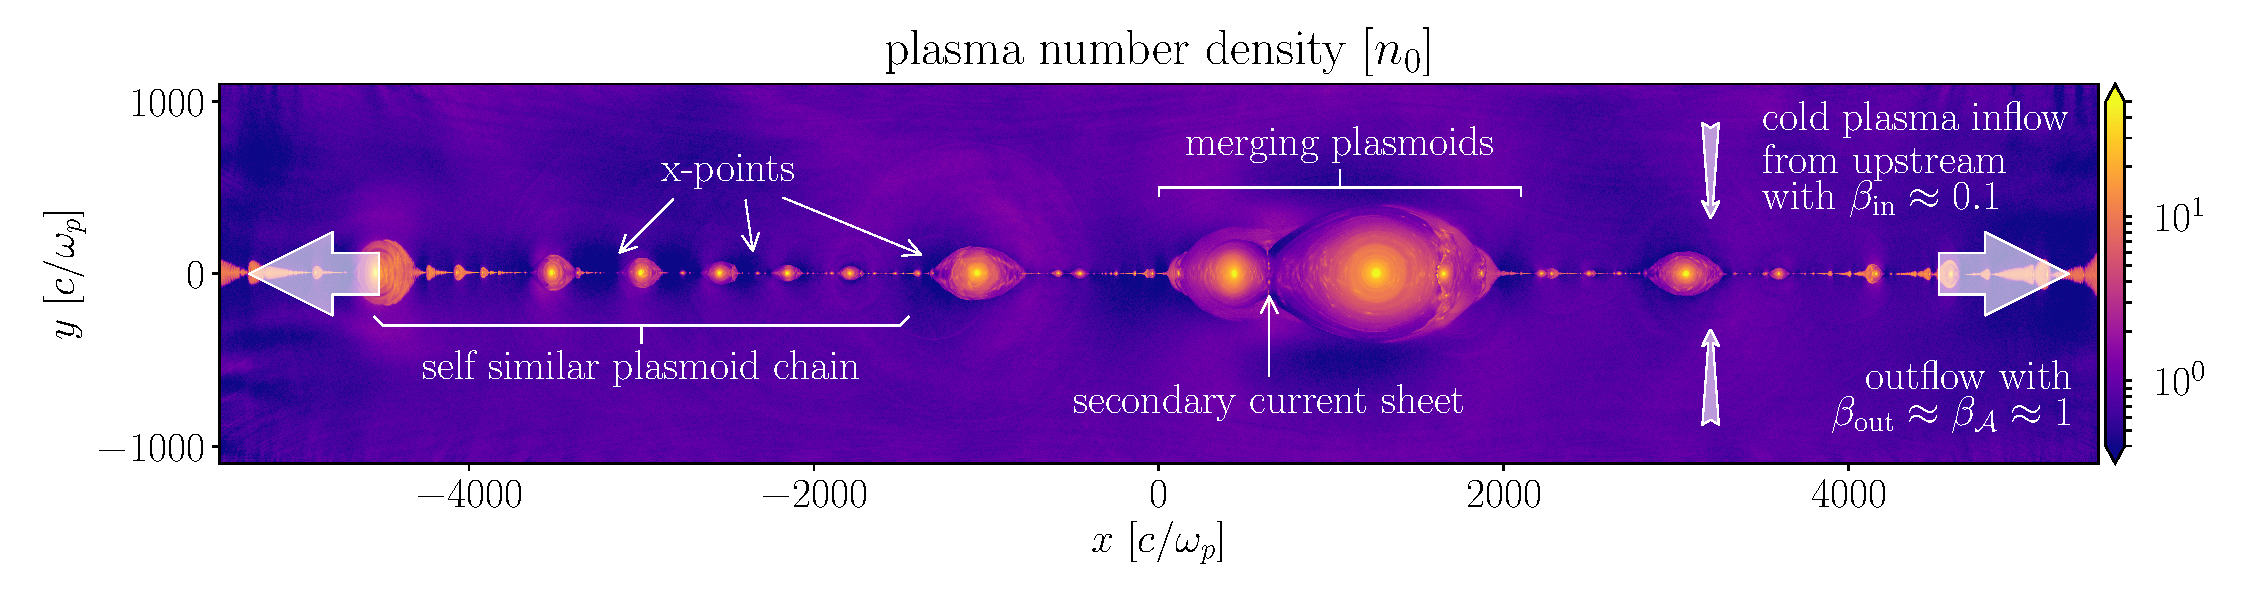
\includegraphics[width=\textwidth]{figures/ch4-pairproduction/fig2.pdf}}
    \caption{Reconnection in two-dimensional box with injection from top and bottom and outflowing boundaries on the left and right. The upstream magnetic field is in the plane of the picture. The color represents the plasma density normalized to the upstream value, $n_0$. $\beta=v/c$ is the typical inflow or outflow velocity. The image is taken from an actual simulation.}
    \label{fig:pairprod-rec_scheme}
\end{figure}

In this section we give a theoretical outline of our work as well as introduce the main terminology and current understanding of how relativistic reconnection works.

\subsection*{\small\it Relativistic reconnection in $e^\pm$ plasma}

It is well known that a current layer separating uniform oppositely directed magnetic field regions is unstable. Plasmoid instability, developing quickly on Alfv\'en crossing timescales, initiates  magnetic reconnection, breaking the current layer into a chain of outflowing plasmoids (see, e.g., \citealt{1997plasconf, 2007PhPl...14j0703L}). Energy of the magnetic field is liberated in this process, which in the relativistic case powers non-thermal particle acceleration, forming a power law spectrum of particles with a cutoff set by the magnetization.\par

% \sasha{Introduce Fig.3 here? In fig.3 we show ...}
In Figure~\ref{fig:pairprod-rec_scheme} we show a typical simulation snapshot of a two dimensional current sheet undergoing the plasmoid instability and reconnection. All the important features, such as the plasmoids, plasmoid mergers, and secondary current sheets are shown in the figure for guidance. The pattern of plasmoids is self-similar on a wide range of scales, and their evolution is stochastic: smallest plasmoids move along the layer with the Alfv\'en velocity (which in relativistic case is close to $c$), but they also merge to become larger and slower, with bulk motions that are just marginally relativistic (for more details see~\citealt{2016MNRAS.462...48S}).

Between the plasmoids, the annihilated magnetic field in the x-points allows the reconnection electric field to accelerate particles. Along with the primary current layer, there are also secondary layers which occur during the plasmoid collisions, serving as additional locations of particle acceleration \citep{2015ApJ...806..167G}. Plasmoids advect hot plasma containing the most energetic particles along the sheet with the Alfv\'en velocity, while the cold upstream plasma, having typically small Lorentz-factors, $\langle\gamma\rangle\approx 1$, inflows with a characteristic velocity $\beta_{\rm in}\equiv v_{\rm in}/c\sim0.1\text{-}0.2$, which corresponds to the reconnection rate. \par

The main dimensionless parameter controlling the dynamics of collisionless relativistic reconnection is the cold magnetization parameter, $\sigma_{\rm c}\equiv (B^2/4\pi) / n m_e c^2$, that sets the available magnetic energy per particle. Here, $n$ is the pair plasma density far from the reconnection layer, where the unreconnected field has the value $B$. When $\sigma_{\rm c}\gg 1$, the majority of particles accelerated in the current layer is typically in the ultra-relativistic regime.
Magnetization controls the maximum energy to which a particle can be accelerated in reconnection. In particular, as was shown by~\cite{2014ApJ...783L..21S} and \cite{2016ApJ...816L...8W}, in the x-point particles can be accelerated up to a few times $\sigma_{\rm c}$. The plasmoids can further accelerate particles, extending the power law to much higher energies \citep{2001ApJ...562L..63Z, 2016MNRAS.462...48S, 2016ApJ...818L...9G, 2018arXiv180800966P}.
%\sasha{may be just say that further acceleration is possible in plasmoid mergers via Fermi process? Also, cite some paper of Fan Guo here.}

In pulsars the value of magnetization, which
%is set by the ratio of Poynting flux to plasma kinetic energy flux,
depends both on the magnetic field strength and the plasma density, can be estimated from the spin down power of the pulsar and the properties of the initial pair production cascade near the polar caps~\citep{1983AIPC..101..163A, 1995phpu.book.....L, 2001ApJ...547..437L, 2010MNRAS.406.1379M, 2010MNRAS.408.2092T}. Typically, this parameter lies between $10^3\text{-}10^5$; for the Crab it can also be directly constrained from PWN observations to be close to $10^4$. This value sets the cutoff energies to which particles can be accelerated.

% \hayk{I just removed this part, I think it won't hurt}

% thus, in terms of our simulations this will correspond to the effective magnetization of the current sheet, $\sigma_{\rm eff}$. When pair production is not involved, this value corresponds to $\sigma_{\rm c}$.

\subsection*{\small\it Particle cooling and photons}

Both electrons and positrons are subject to radiation cooling at relativistic energies. In this work we only consider synchrotron cooling, while  inverse-Compton (IC) cooling may also be important in some contexts~\citep{2018arXiv180501910W}. If the synchrotron cooling time is shorter than the acceleration time (we call this a strong cooling regime), accelerated particles will quickly lose their gained energy in the large background magnetic field without having a chance to reaccelerate again. Unlike the case without cooling, the highest energy particles will no longer be located within the plasmoids, since the plasmoids have typically higher magnetic fields, and the particles within them are efficiently cooled. Instead, most of the high energy particles will be piled up in the vicinity of plasmoids and along the primary and secondary current layers where the magnetic field is close to zero; the maximum energy will thus no longer be set by the plasmoid sizes. Even when synchrotron cooling is strong, the particle energy cutoff will be close to a few times $\sigma_{\rm c}m_e c^2$, as these particles would still accelerate in the primary and secondary current sheets where the local cooling is inefficent.

% Thus, a mechanism described, where particles can reaccelerate to much higher energies in large plasmoid mergers will no longer work.

%\sasha{you don't seem to say why you can accelerate to that energies even in the "strong" cooling case. Because cooling is still slow when B gets to zero in X-points / current sheets}

The cooling regime is parametrized by the value of the Lorentz-factor of particles, $\gamma_{\rm rad}$, for which the radiation drag force is comparable to the accelerating force (for the accelerating electric field we assume $E \sim \beta_{\rm rec} B_0$; hereafter, we use subscript ``0" for upstream values):
\begin{equation}
    \label{eq:pairprod-def_gammarad}
    2\sigma_{\rm T}\frac{B_0^2}{8\pi}\gamma_{\rm rad}^2 = e\beta_{\rm rec}B_0,
\end{equation}
where $\beta_{\rm rec}\approx 0.1$ is the steady-state reconnection rate, and $\sigma_{\rm T}$ is the Thomson cross section.

%As we demonstrate  below using simulations, the particular choice of $\gamma_{\rm rad}$ is not important as long as for highest energy particles with $\gamma>\sigma_{\rm c}$ the cooling time is shorter than the acceleration time, i.e., $\gamma_{\rm rad}\lesssim \sigma_{\rm c}$.

The radiation from a single plasma particle is described by the synchrotron spectrum, peaking at frequency $\omega_{\rm syn}\approx eB_0\gamma^2 / m_e c$. An important benchmark energy for pair production is the electron (positron) rest-mass energy, $m_e c^2$, which determines the minimum center-of-momentum energies for two photons to pair produce. We are, thus, interested to know which plasma particles radiate photons with characteristic energies close to $m_e c^2$. This sets another dimensionless parameter -- the Lorentz-factor of these particles, $\gamma_c$, determined by
\begin{equation}
    \label{eq:pairprod-def_gammac}
    \hbar \frac{e B_0 \gamma_c^2}{m_e c}= m_e c^2.
\end{equation}

Combined together, the cold magnetization parameter of the upstream, $\sigma_{\rm c}$, radiation-reaction limit, $\gamma_{\rm rad}$, and the pair threshold parameter, $\gamma_c$, give the full description of the synchrotron-cooled reconnection problem. We can rewrite the definitions as
\begin{equation}
\label{eq:pairprod-def_gammas}
    \gamma_{\rm rad}^2 \equiv \frac{3\beta_{\rm rec}}{2}\frac{B_{\rm cl}}{B_0},~~~
    \gamma_c^2 \equiv \frac{\alpha B_{\rm cl}}{B_0} = \frac{B_{\rm S}}{B_0},
\end{equation}
where $\alpha$ is the fine-structure constant, $1/137$, $B_{\rm cl}=m^2 c^4/e^3$ is the classical magnetic field, and $B_{\rm S}=m_e^2 c^3/e\hbar$ is the Schwinger field.

For a typical pulsar with the magnetic field at the light cylinder $B_0 = B_{\rm LC} \sim 10^{5}$ G, we find
\begin{equation}\label{eq:pairprod-rad_c_values}
    \gamma_{\rm rad} \approx 10^5 \left(\frac{B_0}{10^{5}~\textrm{G}}\right)^{-1/2},~~~
    \gamma_c \approx 2\cdot 10^4 \left(\frac{B_0}{10^{5}~\textrm{G}}\right)^{-1/2}.
\end{equation}
For the Crab, with $B_{\rm LC}\sim 4\times 10^6$ G, these values are $\gamma_{\rm rad}\approx 10^4$ and $\gamma_c\approx 3\times 10^3$~\citep{2014ApJ...780....3U}, and the typical magnetization near the light cylinder is $10^4\text{-}10^5$. We, thus, have a hierarchy of energy scales with $\gamma_c \ll \gamma_{\rm rad} \lesssim \sigma_{\rm c}$, which we will use in our simulations.

\subsection*{\small \it Two-photon pair production}

Two photons can interact through the Breit-Wheeler process to form an electron-positron pair, $\gamma\gamma\to e^-e^+$ \citep{PhysRev.46.1087}. This can happen if the center-of-momentum energy of photons is greater than the rest-mass energy of the electron-positron pair
\begin{equation}
    \label{eq:pairprod-def_s}
    s \equiv \frac{1}{2}\frac{\varepsilon_1\varepsilon_2}{(m_e c^2)^2} (1-\cos{\phi}) > 1,
\end{equation}
where $\varepsilon_1$ and $\varepsilon_2$ are the lab frame photon energies, and $\phi$ is the angle between their momenta. The cross section for this interaction behaves as $\sqrt{s-1}$ near $s\gtrsim 1$, peaks around $s\approx 2$ and drops down as $1/s$ for $s\gg 1$. In Figure~\ref{fig:pairprod-sigma_pp} we show the magnitude of this cross section plotted vs the relative angle of two interacting photons, $\phi$, and the product of their energies measured in $m_ec^2$. White shaded region corresponds to values of $s$ where pair production is not possible.

Figure \ref{fig:pairprod-sigma_pp} demonstrates two important facts: the high energy photons ($\varepsilon \gg m_e c^2$) pair produce preferentially with the lower energy ones ($\varepsilon \ll m_e c^2$), while the ones with intermediate energies ($\varepsilon \approx m_e c^2$) pair produce with each other. Also, the small angle interactions with $\phi\approx 0$ are suppressed, while the head-on collisions, $\phi\approx \pi$, are more preferred.

\begin{figure}[htb]
    \sidebysidecaption{0.555\linewidth}{0.42\linewidth}{
        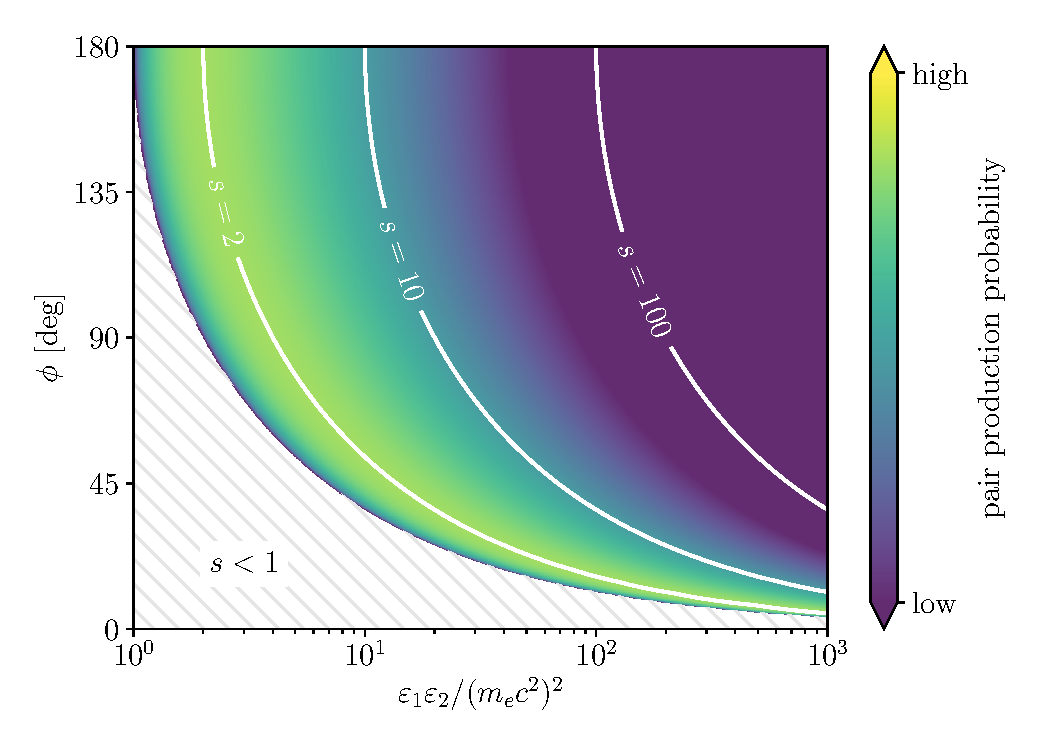
\includegraphics[width=\textwidth]{figures/ch4-pairproduction/fig3.pdf}
    }{
        \caption{Two-photon pair production cross section as a function of the angle between their momenta, $\phi$, and the product of photon energies in units of $m_e c^2$. The pair production probability is highest when the center-of-momentum energy is $\approx \sqrt{2}m_e c^2$. For small angles only the most energetic photons can pair produce with each other, while head-on interactions allow a wider range of energies.}
        \label{fig:pairprod-sigma_pp}
    }
\end{figure}

We will consider a system to be optically thin to two-photon pair production, $\tau_{\gamma\gamma}\ll 1$, if at all energies only a small fraction of photons is converted to pairs. This means that most of the photons stream freely out of the system without any interactions. Note also, that this condition is hardest to satisfy for the highest energy photons, since they typically have a high pair production probability while streaming through a dense background of low energy radiation.

In an optically thin regime for a power-law energy distribution of photons one can show that photons in a wide range of energies contribute roughly equally to pair production. If the photon energy cutoff is at $\varepsilon_{\rm max}$, all the photons from $\varepsilon_{\rm min} \approx (m_e c^2)^2/\varepsilon_{\rm max}$ to $\varepsilon_{\rm max}$ are equally important to consider. This makes the problem of photon tracking numerically challenging. On the other hand, very low energy photons, $\varepsilon \ll \varepsilon_{\rm min}$, have no high energy partner to interact with, and can thus be thrown out of consideration in the context of pair production.

\subsection*{\small \it Steady state and the effective secondary plasma density}

\begin{figure}[tb]
    \sidebysidecaption{0.555\linewidth}{0.42\linewidth}{
        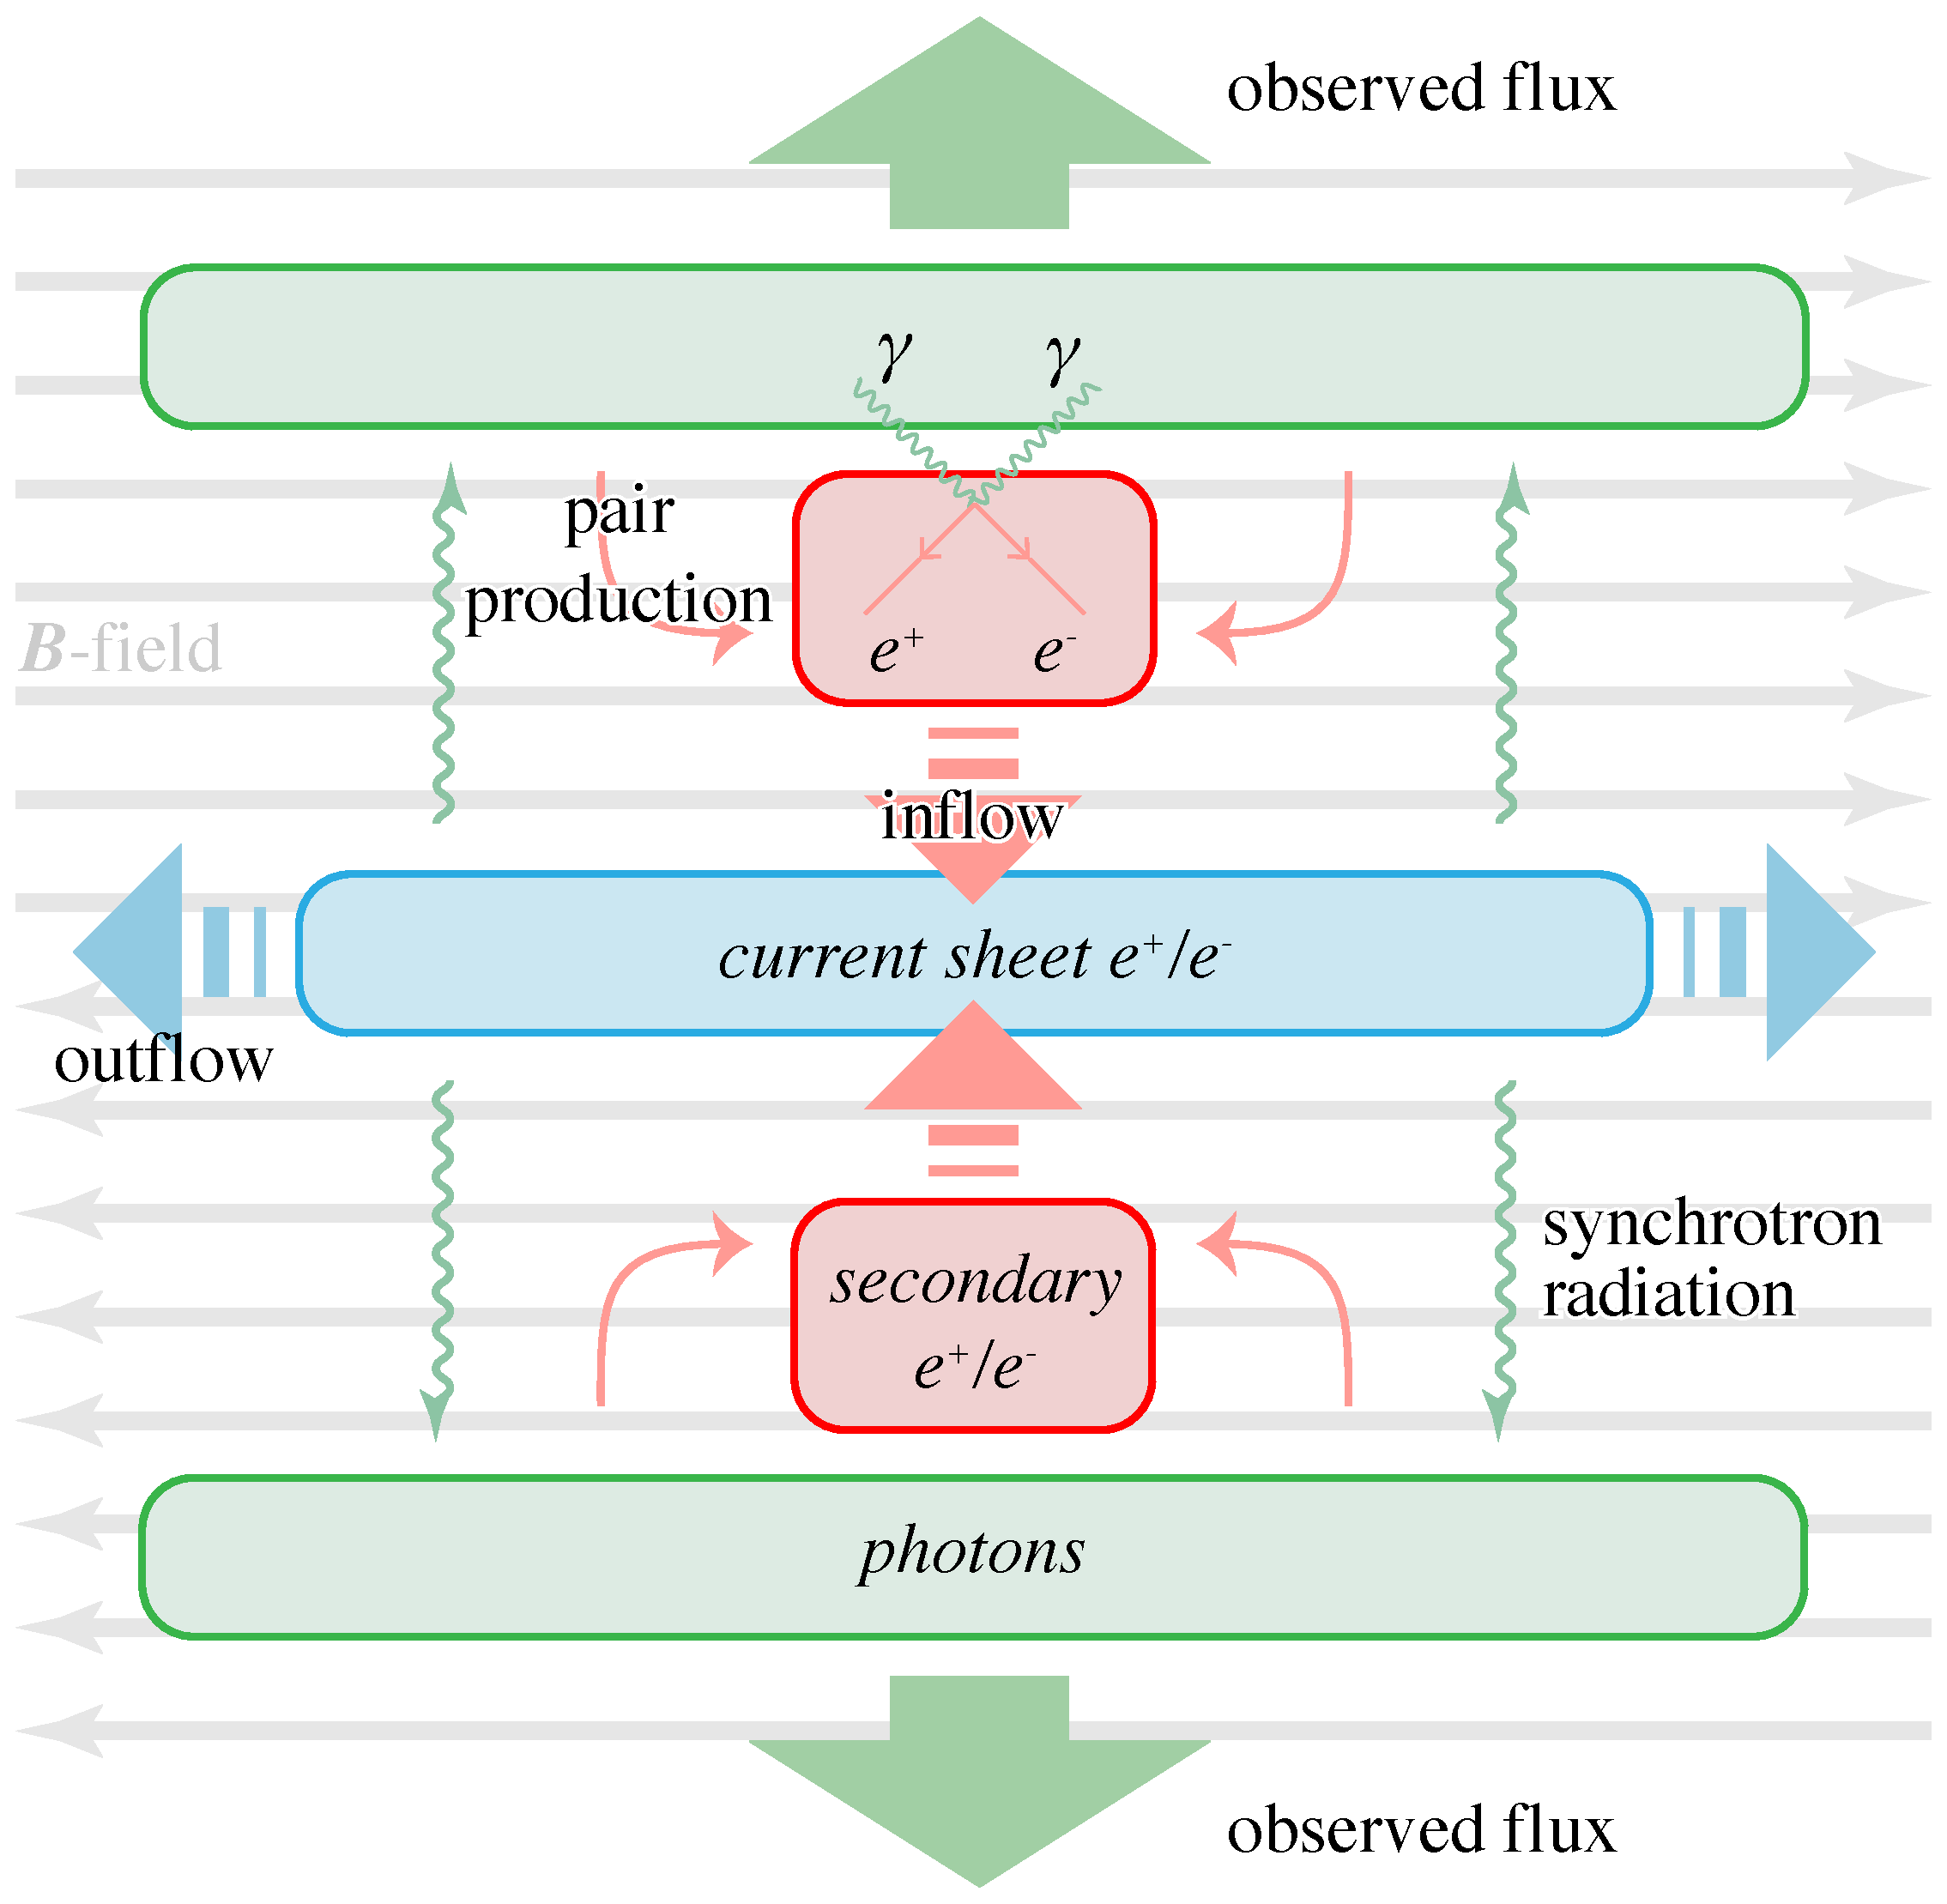
\includegraphics[width=\textwidth]{figures/ch4-pairproduction/fig4.pdf}
    }{
        \caption{Schematic illustration of the reconnecting current sheet in its steady state. Plasma in the current sheet cools down via synchrotron radiation. These photons later pair produce in the upstream, and secondary pairs are advected into the current sheet.}
        \label{fig:pairprod-steady_state}
    }
\end{figure}

We now describe a simple model of reconnection with synchrotron cooling and pair production to better illustrate the pair loading feedback mechanism and the steady state. We also predict the steady state multiplicity of secondary plasma in our simulations and in $\gamma$-ray pulsars, and it's dependence on the background magnetic field.

The general picture is schematically shown in Figure~\ref{fig:pairprod-steady_state}, where we show how different ingredients of reconnection work together to build up the feedback and ultimately drive the system to a steady state. Most of the plasma resides in the current sheet (blue region in Fig.~\ref{fig:pairprod-steady_state}), where it gets accelerated and radiates a power law distribution of photons $\mathrm{d}n_\gamma/\mathrm{d}\varepsilon_\gamma\propto\varepsilon_\gamma^{-\Gamma}$. Each particle experiences a radiative drag force and loses its energy to radiation at the rate
\begin{equation}
    \label{eq:pairprod-sync_rate}
    \dot{\epsilon} = 2\sigma_{\rm T} c \frac{B_0^2}{8\pi}\gamma^2 = e c \beta_{\rm rec} B_0 \left(\frac{\gamma}{\gamma_{\rm rad}}\right)^2,
\end{equation}
where $\gamma_{\rm rad}$ is defined in Eq.~(\ref{eq:pairprod-def_gammarad}).

We will assume that each particle with energy $\gamma m_e c^2$ radiates photons with synchrotron peak frequency in the fixed upstream field $B_0$:
\begin{equation}
    \label{eq:pairprod-sync_peak}
    \varepsilon_\gamma = m_e c^2\left(\frac{\gamma}{\gamma_c}\right)^2,
\end{equation}
where $\gamma_c$ is defined in Eq.~(\ref{eq:pairprod-def_gammac}). The radiated photons pair produce in the upstream, creating secondary pairs that feed the current sheet further. The total photon production rate can be found from  equations (\ref{eq:pairprod-sync_rate}) and (\ref{eq:pairprod-sync_peak}):
\begin{equation}\label{eq:pairprod-photon_rate}
    \dot{n}_\gamma = \frac{\dot{\epsilon} (n_{\rm sec} + n_0)}{\varepsilon_\gamma} = \frac{e c \beta_{\rm rec} B_0 n_0 (1+\eta)}{m_e c^2}\left(\frac{\gamma_c}{\gamma_{\rm rad}}\right)^2,
\end{equation}
where we defined the multiplicity, $\eta$, as the ratio of the secondary plasma density to that of the primary, $n_{\rm sec} / n_0$.

Given the spectrum of photons we can find how the number of pair producing photons scales with the spectral cutoff
\begin{equation}\label{eq:pairprod-photon_pp_scale}
    \tilde{n}_\gamma \propto \int\limits_{\varepsilon_{\rm min}}^{\varepsilon_{\rm max}}\varepsilon_\gamma^{-\Gamma}\mathrm{d}\varepsilon_\gamma \propto \varepsilon_{\rm min}^{1-\Gamma}\propto \varepsilon_{\rm max}^{\Gamma - 1},
\end{equation}
where we used the fact, that $\varepsilon_{\rm min}\varepsilon_{\rm max}\approx (m_e c^2)^2$.

% We will assume that most of the photon-to-photon collisions are head-on. This means, that the center-of-momentum energy of photons given by Eq.~(\ref{eq:pairprod-def_s}) is $s\approx \varepsilon_1\varepsilon_2 / (m_e c^2)^2$. Since pair production cross section peaks when $s\approx 2$, the lowest energy photons (with $\varepsilon_\gamma\ll m_e c^2$) pair produce with the highest energy ones (with $\varepsilon_\gamma\gg m_e c^2$), while the intermediate energy photons ($\varepsilon_\gamma\approx m_ec^2$) pair produce with each other. Moreover, the contribution of all energy bins is roughly the same (see details in the appendix~\ref{sec:appendixB}).

Photons of the highest energies are radiated by the particles with the highest Lorentz-factors. Reconnection accelerates particles up to a few times $\sigma$, which is lower than the initial value $\sigma_0=B_0^2/4\pi n_0 m_e c^2$ by a factor of $(1+\eta)$. Thus, when the multiplicity grows, the effective magnetization and the maximum photon energy decrease, shrinking the energy band of pair producing photons (decreasing $\tilde{n}_{\gamma})$. This is the pair production feedback that drives the system to a self-regulated steady state.

To estimate the steady state multiplicity we can write the pair production rate as follows:
\begin{equation}\label{eq:pairprod-pair_rate}
    \dot{n}_{\rm sec} \approx \sigma_{\rm T} c \tilde{n}_\gamma^2 f_0,
\end{equation}
where the dimensionless parameter $f_0$ sets the interaction cross section, $\sigma_{\gamma\gamma} = f_0 \sigma_{\rm T}$, and depends on the energies and momenta of interacting photons. The peak value of $f_0$ is close to $0.3$; we will take an empirical value of $0.1$. The final result depends weakly on this parameter.

In steady state both the secondary plasma and the photons are advected out of the reconnection region. Our simplified model is purely one-dimensional: the system extends infinitely in the horizontal and out-of-plane directions in Figure~\ref{fig:pairprod-steady_state}, while the only variation appears in the direction perpendicular to the current sheet (vertical direction in the figure). We then introduce two length-scales in this direction in the current sheet inflow domain: $s_1$ -- the region where most of the photon radiation happens, and $s_2$, where most of the pair production events take place. We can then convert the production rates to steady-state densities:
\begin{equation}\label{eq:pairprod-def_scales}
    n_\gamma = \dot{n}_{\gamma} s_1 / c,~~~n_{\rm sec} = \dot{n}_{\rm sec} s_2 / c.
\end{equation}
Combining Eq.~(\ref{eq:pairprod-photon_rate}-\ref{eq:pairprod-def_scales}) we find
\begin{equation}
\begin{split}
    n_{\rm sec} = n_0 \eta & =
                    \beta_{\rm rec}^2 f_0 \frac{\sigma_{\rm T} e^2 B_0^2 n_0^2}{(m_e c^2)^2} s_1^2 s_2 \times \\
                    & \times (1+\eta)^2\left(\frac{\varepsilon_{\rm max}}{m_e c^2}\right)^{2\Gamma-2}\left(\frac{\gamma_c}{\gamma_{\rm rad}}\right)^4,
\end{split}
\end{equation}
where we set $\tilde{n}_\gamma = n_{\gamma}(\varepsilon_{\rm max}/m_e c^2)^{\Gamma-1}$. We can then take $\varepsilon_{\rm max}/m_e c^2 = (\sigma/\gamma_c)^2$, with $\sigma = \sigma_0 / (1 + \eta)$, and substitute $n_0 = B_0^2 / 4\pi \sigma_0 m_e c^2$. After some simplification we get
\begin{equation}
    \frac{\eta}{(1+\eta)^{6-4\Gamma}} =
            \frac{\beta_{\rm rec}^2 f_0}{4\pi}
            \frac{\sigma_{\rm T} e^2 B_0^4}{(m_e c^2)^3}s_1^2 s_2
            \frac{\gamma_c^{8-4\Gamma}}{\gamma_{\rm rad}^4\sigma_0^{5-4\Gamma}}.
\end{equation}

To express this relation through dimensionless numbers let us substitute $\sigma_{\rm T}$ from~(\ref{eq:pairprod-def_gammarad}) and define the cold plasma gyroradius as $\rho_0 = m_e c^2 / e B_0$. We can then rewrite the expression above:
\begin{equation}\label{eq:pairprod-sim_mult_theory}
    \frac{\eta}{(1+\eta)^{6-4\Gamma}} =
            \beta_{\rm rec}^3 f_0
            \frac{s_1^2 s_2}{\rho_0^3}
            \frac{\gamma_c^{8-4\Gamma}}{\gamma_{\rm rad}^6\sigma_0^{5-4\Gamma}},
\end{equation}
or, assuming $\eta \gg 1$,
\begin{equation}\label{eq:pairprod-sim_mult_theory2}
    \eta = \left(\beta_{\rm rec}^3 f_0\right)^{1/(4\Gamma-5)}
            \left(\frac{s_1^2 s_2}{\rho_0^3}\right)^{1/(4\Gamma-5)}
            \frac{\sigma_0}{\gamma_{\rm rad}^{6/(4\Gamma-5)}\gamma_c^{(4\Gamma-8)/(4\Gamma-5)}}.
\end{equation}
We will compare this estimate with our simulations in section \S\ref{sec:pairprodaccell} where we describe our results.

In $\gamma$-ray pulsars the power law index of photons is close to $\Gamma\approx 1\text{-}2$ \citep{2013ApJS..208...17A}. To estimate the multiplicity near the light cylinder, we can use the values of $\gamma_c$ and $\gamma_{\rm rad}$ defined in Eq.~(\ref{eq:pairprod-rad_c_values}) and take $n_0 = \kappa n_{\rm GJ}$, where $\kappa\approx 10^4$ is the multiplicity of the primary cascade near the polar cap, and $n_{\rm GJ}\approx\Omega B_0 / 2\pi c e$. We will also assume that $s_1 = s_2 \approx 0.1 R_{\rm LC}$. We then find, for $\Gamma=2$, that
\begin{equation}\label{eq:pairprod-obs_mult_theory}
    \eta \approx 2\times 10^4~
    \left(\frac{B_{\rm LC}}{10^5~\text{G}}\right)^{3}
    \left(\frac{P}{100~\text{ms}}\right)^{2}
    \frac{(s_1^2 s_2)^{1/3}}{0.1~R_{\rm LC}}.
\end{equation}
In particular, for the Crab ($B_0\sim 10^6$ G, $P=33$ ms) we find $\eta\sim 10^5\text{-}10^6$ for $\Gamma=2$. Thus, we expect pair loading to significantly affect reconnection near the Y-point.

% (as seen on Figure~\ref{fig:snapshot}).

\section{Reconnection with cooling and pair production: simulations}
\label{sec:pairprod-results}

\subsection*{Simulation setup}

We set up a 2D relativistic particle-in-cell simulation of a reconnecting current sheet using the code \texttt{TRISTAN-MP} \citep{2005AIPC..801..345S}. The current sheet is initially in Harris equilibrium: cold (Maxwellian) upstream plasma with no bulk motion and a current sheet with hot plasma and bulk current (electrons and positrons having bulk velocities in opposite direction) to balance the magnetic field. The sheet is perturbed by either the artificial cooling of the central region or by adding a temporary magnetic loop near the center (see, e.g.,~\citealt{2018MNRAS.473.4840W}). In either case, the evolution does not depend on the way we trigger reconnection, and the later steady state behavior is completely determined by our initial parameters.

Reconnection rapidly develops into the non-linear stage where plasmoids are formed, advecting magnetic field loops and particles out of the box. While in one direction the absorbing boundary conditions allow plasma and fields to flow out (left and right boundaries on Figure~\ref{fig:pairprod-rec_scheme}), in the other direction the boundaries are being constantly extended while injecting seed primary plasma at rest in the far upstream (for more details see~\citealt{2014ApJ...783L..21S}). This approach eliminates reflections from the boundaries. In the third unmodeled dimension the boundary conditions are periodic.

The box size, $L$, is chosen so that $L/\sigma\rho_0 \gtrsim 50$, where $\rho_0$ is the gyroradius of a low energy particle in the upstream field, and $\sigma$ is either the initial upstream magnetization parameter, $\sigma_0$, or, in the case of pair production, the effective magnetization, $\sigma_{\rm eff}$, which is much lower due to the mass loading by secondary pairs. After the reconnection starts, we wait until the transient plasmoids are advected out of the box, and the steady state is reached, and then turn on the cooling and pair production. We then wait for a few light-crossing times of the box until a new steady state is reached.

A charged ultra-relativistic particle ($\gamma\gg 1$, $\beta\approx 1$) in electromagnetic field experiences the radiation drag force (see, e.g., \citealt{1975ctf..book.....L})
\begin{equation}
\label{eq:pairprod-drag}
    \bm{F} = -\frac{2}{3}r_e^2\gamma^2\bm{\beta}\left[\left(\bm{E}+\bm{\beta}\times\bm{B}\right)^2 - \left(\bm{\beta}\cdot\bm{E}\right)^2\right],
\end{equation}
where $r_e$ is the classical radius of the electron, and radiates synchrotron photons. In our simulations we define the effective perpendicular magnetic field,
\begin{equation}
    B_{\rm eff}^2=\left(\bm{E}+\bm{\beta}\times\bm{B}\right)^2 - \left(\bm{\beta}\cdot\bm{E}\right)^2,
\end{equation}
which we will further use to compute the photon energy and the cooling rate. When the synchrotron cooling is enabled, each particle in our simulation probabilistically radiates a photon at the corresponding synchrotron frequency set by the pair threshold parameter, $\gamma_c$,
\begin{equation}
    \label{eq:pairprod-synch_form}
    \varepsilon_{\rm sync} = m_e c^2\left(\frac{\gamma}{\gamma_c}\right)^2\left(\frac{B_{\rm eff}}{B_0}\right)\left(\frac{\sigma_0}{10^3}\right)^{1/2},
\end{equation}
where $B_0$ is the upstream magnetic field, and the last factor takes into account the magnetic field normalization, i.e., $\varepsilon_{\rm sync}\propto \gamma^2 B_0$. The photon radiation probability is set in such a way that the overall cooling rate, or the energy lost by a particle in a timestep, is consistent with the drag force in formula (\ref{eq:pairprod-drag}) and is controlled by $\gamma_{\rm rad}$:
\begin{equation}
    \label{eq:pairprod-synch_rate}
    \frac{\Delta \varepsilon}{\Delta t} \propto \left(\frac{\gamma}{\gamma_{\rm rad}}\right)^2 \left(\frac{B_{\rm eff}}{B_0}\right)^2.
\end{equation}\par
% On the other hand, the number of produced photons per timestep, and thus the energy of each photon is set by $\gamma_c$ and is also consistent with the particle momentum and the magnetic field \sasha{should we write an explicit equation here for the emission probability and photon energy? That would be better than these long sentences}.
Our simulation tracks photons as regular chargeless and massless particles propagating along straight lines with speed $c$. We do not track photons with very low energies (typically lower than $0.1\text{-}1\%$ of $m_e c^2$), since they do not significantly contribute to pair production (for details see appendix~\ref{sec:pairprod-appendixB}); they are, however, accounted for in particle cooling.

In each cell, every pair of photons can pair produce with a certain probability. We compute these binary probabilities for each pair of photons in the same cell according to Breit-Wheeler cross section and probabilistically create electron-positron pairs in that cell with momenta consistent with the differential cross section of the process. This algorithm naturally conserves both momentum and energy. Since we loop through all pairs of photons in each cell, this automatically ensures that the mean free path of every photon is inversely proportional to the number density of photons.

Magnetic reconnection in real astrophysical environments is controlled by a combination of the inflowing plasma density and the background magnetic field. Corresponding synchrotron energy is coupled to these parameters through the Planck's constant, $\hbar$, while pair production cross section magnitude is set by the Thomson cross section, $\sigma_{\rm T}$. Particle-in-cell simulations without radiation can be made dimensionless by normalizing simulation parameters to plasma length- and time-scales. Radiation and pair production introduce two extra scales (set by $\hbar$ and two-photon interaction cross section). We thus have four dimensionless parameters in our simulations:
\begin{itemize}

    \item The cold upstream magnetization parameter, $\sigma_{\rm c} = \sigma_0$, and the radiation-reaction limit, $\gamma_{\rm rad}$, set the background magnetic field and the effective plasma density, determining the available magnetic energy budget per particle and the rate with which particle energy is being transferred to radiation.

    \item The pair threshold parameter, $\gamma_c$, sets the scale of the Schwinger field, $B_{\rm S}$, with respect to the background magnetic field through relation (\ref{eq:pairprod-def_gammas}). Given the total energy deposited into radiation (which is set by $\sigma_0$ and $\gamma_{\rm rad}$), this parameter determines how this energy is distributed between photons, defining the Lorentz-factor of the particle that radiates an MeV photon in the upstream field, as defined in equation (\ref{eq:pairprod-def_gammac}).
% \sasha{again, too many words. may be add an equation that clarifies?} \hayk{I just don't want to write the same equation 2 times}%, defining the position of the synchrotron peak.

    \item The effective mean free path to pair production is set by the fiducial dimensionless parameter $p_0$. In particular, the probability for two photons to produce $e^-e^+$ pair in one timestep is
    \begin{equation}
        p(\Delta t)=p_0\frac{\sigma_{\gamma\gamma}}{\sigma_{\rm T}},
    \end{equation}
    where $\sigma_{\gamma\gamma}$ is the Breit-Wheeler cross section that depends on momenta and energies of the two photons, and $\sigma_{\rm T}$ is the Thomson cross section. We choose a particular value of $p_0$ to ensure the small optical thickness of the overall system, while still producing enough secondary plasma. In Appendix~\ref{sec:pairprod-appendixA} we discuss in more detail how varying this parameter affects the regime we are simulating. 
\end{itemize}

In order to accurately sample the photon momentum space in our typical runs, we would require on average $10^3\text{-} 10^5$ photons per cell. To make this problem computationally feasible, we introduce ``weights'' for each photon and a merging routine to combine them. We use the algorithm described by \cite{2015CoPhC.191...65V} that merges all photons in the same momentum bin (and the same cell) to produce two ``heavy'' photons, while conserving energy and momentum without introducing any unnecessary momentum spread. Our momentum bins are uniform in direction and logarithmic in energy. To avoid artificial effects of binning, such as clumping of momenta in a particular direction, we change the orientations and sizes of these bins with times.

The disadvantage of this photon merging process is that it artificially decreases the pair production efficiency, since photons merged into a single ``heavy'' photon can no longer pair produce with each other. This turns out to have a weak effect on the results, since all the merged photons have small angles between their momenta and small relative energies, and so they have a small interaction probability according to Figure~\ref{fig:pairprod-sigma_pp}. While photon merging is as expensive as pair production in terms of computational time, it is crucial to implement to reduce the memory usage. As a result, we can reduce the number of photons by a factor of $10\text{-}100$, while keeping the overall energy and momentum conserved and not affecting strongly the pair production.

In addition, we make several compromises in order to reduce both the time and memory consumption.
%, which do not, however, significantly affect the overall results.
Synchrotron cooling makes plasmoids effectively compressible, and in the strong cooling regime the centers of plasmoids may get very high overdensities where the local skin depth becomes unresolved:
\begin{equation}
    \frac{c/\omega_{\rm p}}{c/\omega_{\rm p0}} = \langle \gamma \rangle^{1/2} \left(\frac{n_0}{n}\right)^{1/2}.
\end{equation}
Here, $\langle \gamma \rangle$ is the mean Lorentz-factor of particles, which is typically of the order of $\sigma_0$ in plasmoid centers, $n/n_0$ is the particle overdensity compared to the upstream, $c/\omega_{\rm p}$ and $c/\omega_{\rm p0}$ are the local and upstream skin depths. To resolve the local skin depth with the same number of cells as in the upstream, we need to prevent overdensities larger than $\sim \sigma_0$. To alleviate this issue, we turn off the cooling in the very centers of plasmoids, where the overdensity compared to the upstream is above a certain value (typically few $\sigma_0$).\footnote{The regions of large density where the cooling is artificially turned off are very small and are located deep in the middle of the plasmoids. We set the overdensity threshold for turning off the cooling, so that this region is just a few skin depths in size. This limiter does not affect the overall dynamics of the plasmoid, since the majority of particles still lie well beyond the very central region.} As a result, the plasma cools down within the plasmoid until it reaches a particular distance from the center below which the cooling is turned off. The hot central region supports the plasmoid against further contraction; this has no noticeable effect on plasmoid motion. Upstream pair production is also not strongly affected by this effect, since the photons emitted in the centers would not escape the plasmoid due to a high optical depth inside. If the cooling were not turned off in the center, radiated photons would pair produce inside the plasmoid, feeding its interior with additional plasma until the plasmoid center cooled down and stopped emitting pair producing photons.
% as higher energy photons will have high optical depth and will pair produce locally within the plasmoid, feeding it further until the plasma cools down enough to stop emitting radiation that is able to pair produce.

We also allow photons to escape into upstream from within the dense regions of plasmoids before they pair produce. This results in the lack of secondary plasma in the plasmoid interiors which, however, does not affect the overall physics, since most of this plasma would be carried away with the plasmoids,  unable to escape upstream.


\begin{figure}[tb]
    \centering
    \centerline{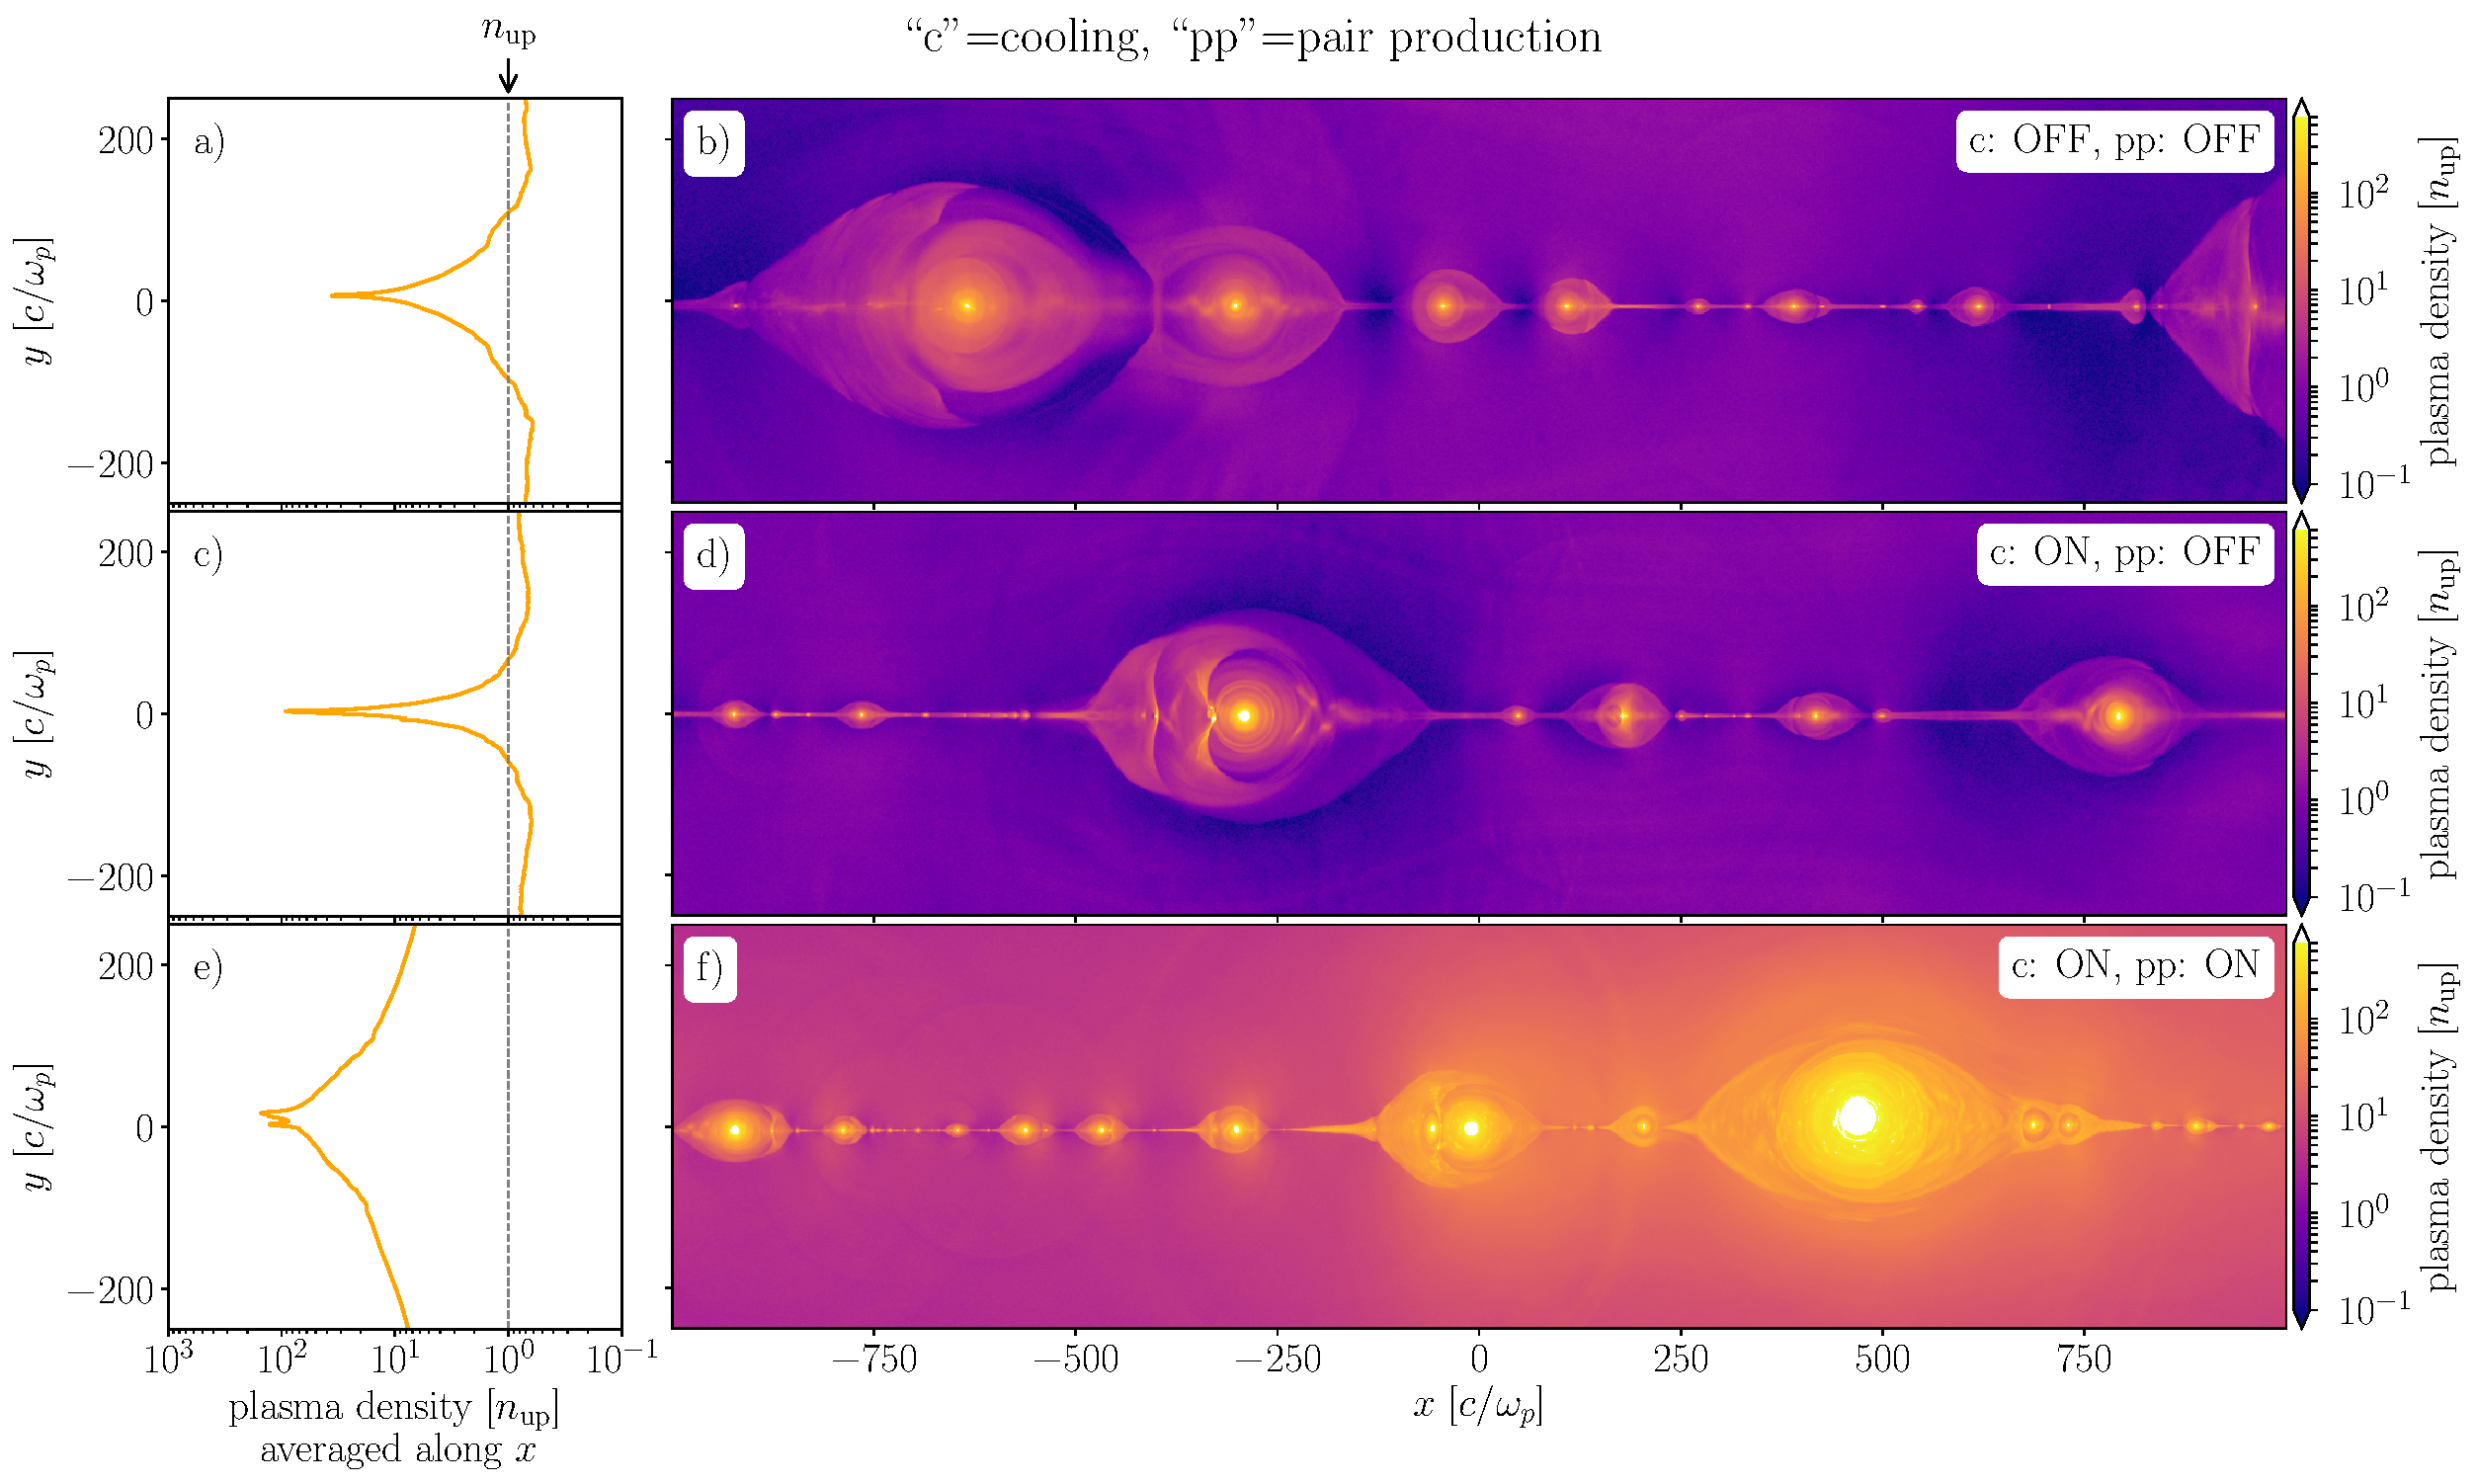
\includegraphics[width=\textwidth]{figures/ch4-pairproduction/fig5.pdf}}
    \caption{Snapshots of plasma density from three different simulations with $\sigma_0=5000$: a-b) without synchrotron cooling or pair production; c-d) with cooling ($\gamma_{\rm rad}=1000$, $\gamma_c=50$) but without pair production; e-f) with both cooling and pair production (additionally $p_0=10^{-5}$). Three plots on the left (panels a, c, e) represent the averaged densities along the current sheet ($x$ axis) plotted vs $y$ axis. Note that all three colorbars as well as the horizontal axes in panels (a, c, e) have the same scale for convenience. When cooling is enabled, plasmoids become effectively compressive, so the typical plasmoid sizes and central overdensities are larger in panel (c) compared to panel (a), where there is no cooling. With pair production enabled (panels e, f) the secondary plasma mass loads both the far upstream and plasmoids, making them larger and heavier.}
    \label{fig:pairprod-snapshot_dens}
\end{figure}

\begin{figure}[tb]
    \centering
    \centerline{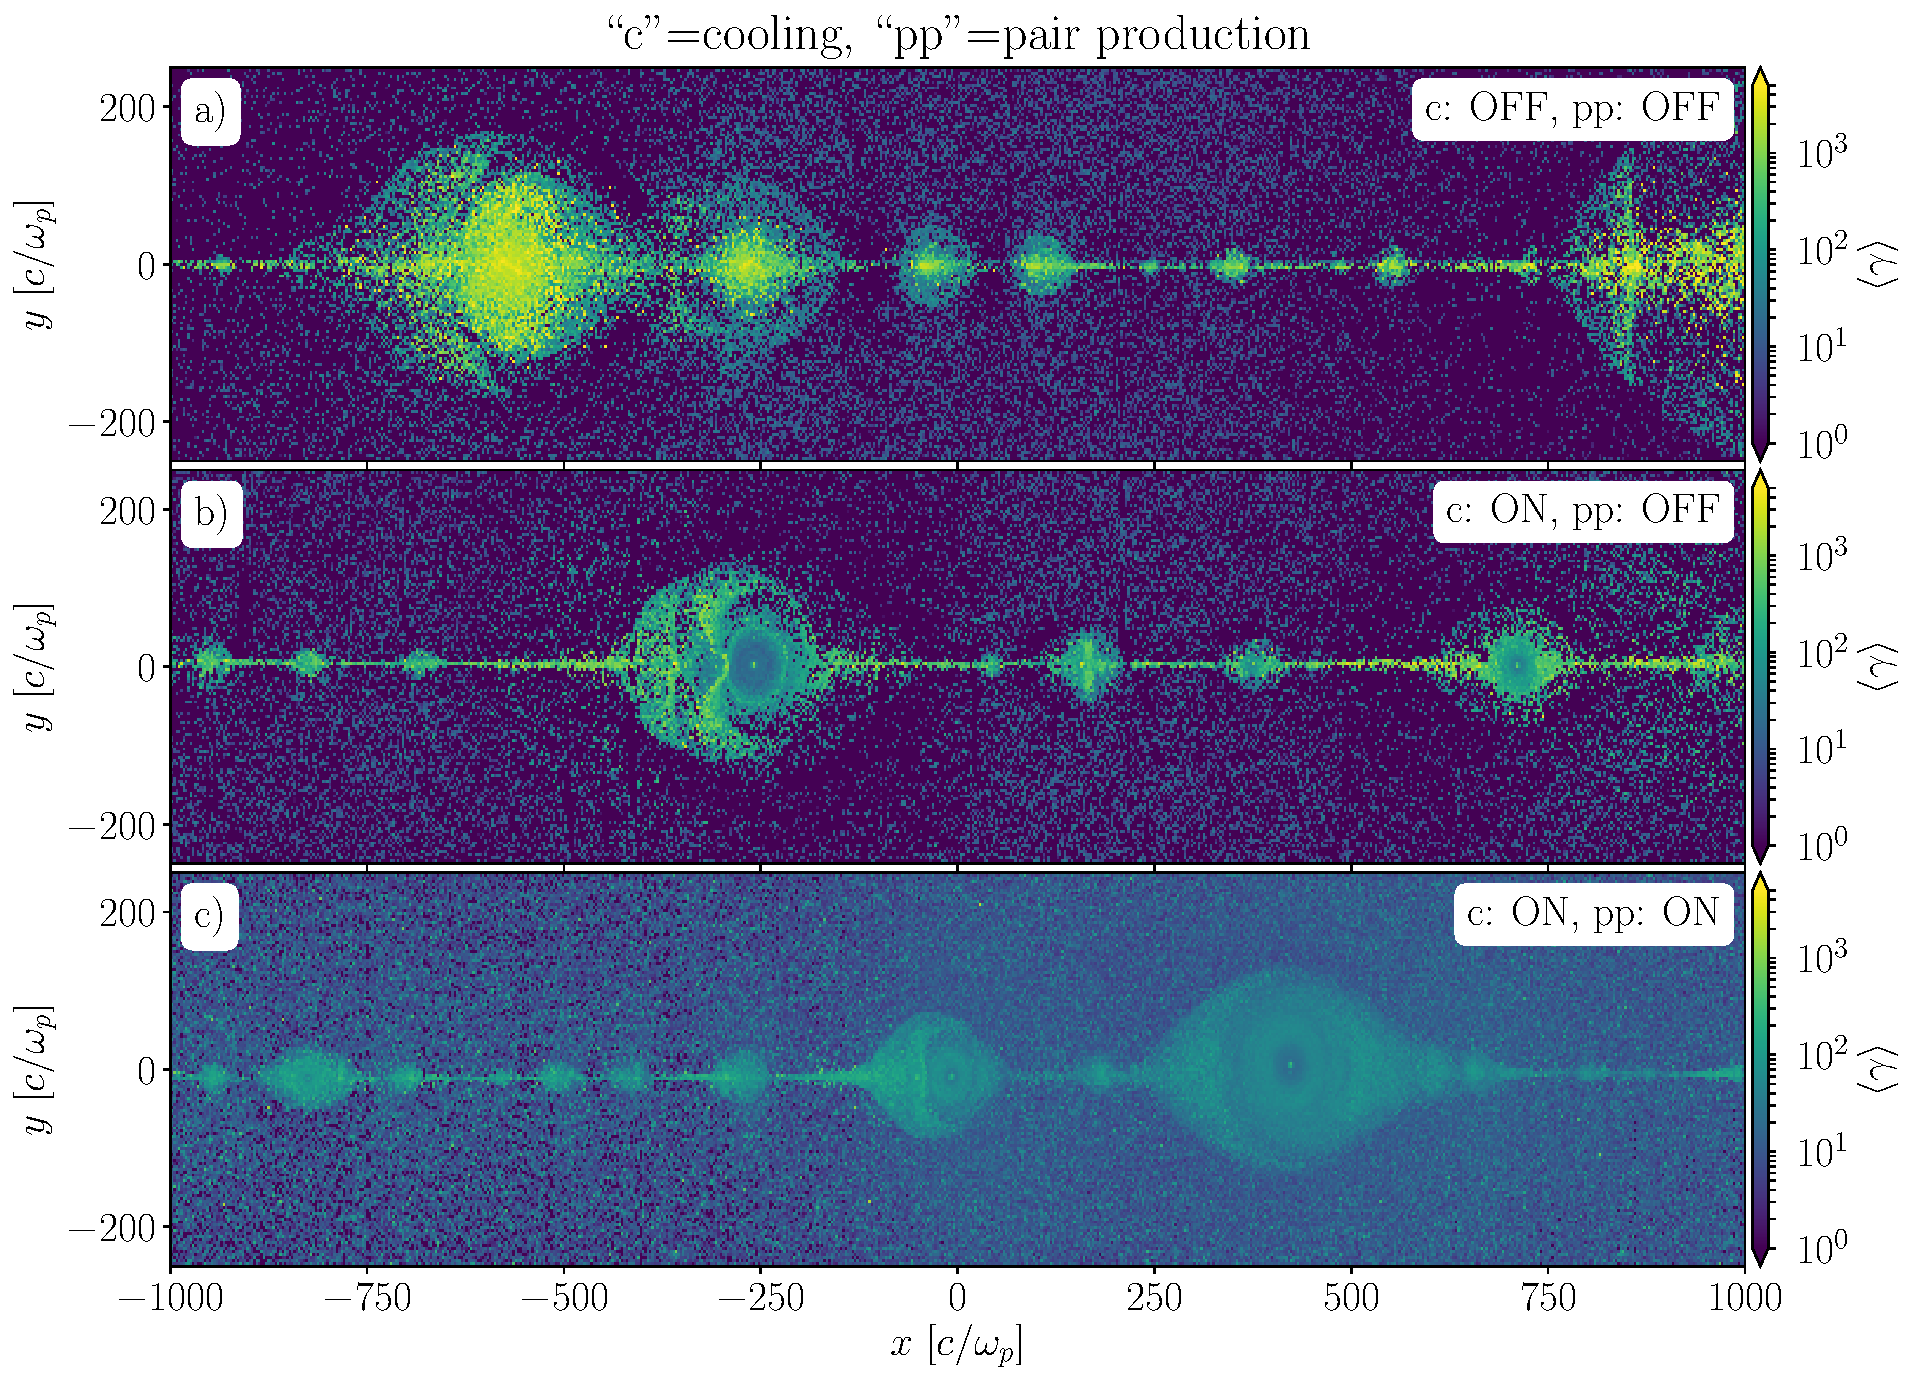
\includegraphics[width=0.85\textwidth]{figures/ch4-pairproduction/fig6.pdf}}
    \caption{Snapshots of the mean particle Lorentz factor from the same three simulations as in Figure~\ref{fig:pairprod-snapshot_dens}. In panel (a) where we present the fiducial run without cooling or pair production, most of the high energy plasma with $\gamma\sim \sigma_0$ is contained within the plasmoids, providing pressure support to resist contraction. When synchrotron radiation is enabled, shown in (b), particles within the plasmoids are efficiently cooled to energies $<\gamma_{\rm rad}$, the pressure support is weaker, and the plasmoids are denser. In this case most of the high energy plasma is contained around the primary current layer, where the magnetic field is weak and the cooling is inefficient. Panel (c) shows the run with pair production, in which case the upstream is hotter, since the newly born secondary pairs inherit the power-law energy distribution from their parent photons.}
    \label{fig:pairprod-snapshot_meang}
\end{figure}
% \new{Snapshots of plasma density from three different simulations with $\sigma_0=5000$, from top to bottom: (A) without synchrotron cooling or pair production, (B) with cooling ($\gamma_{\rm rad}=1000$, $\gamma_c=50$) but without pair production, (C) with both cooling and pair production (additionally $p_0=10^{-5}$). Three plots on the left represent the averaged densities along the current sheet ($x$ axis) plotted vs $y$ axis in all three cases. Note that all three colorbars as well as horizontal axes on three left panels have the same scale. When cooling is enabled (panel B), plasmoids become effectively compressive, so the typical plasmoid sizes and central overdensities are higher on panel B, than on panel A, where there is no cooling. With pair production enabled (panel C) the secondary plasma produced in $\gamma+\gamma$ interactions is produced in the upstream, mass loading both the far upstream and plasmoids, making them effectively larger and heavier.}

% A steady state is reached in our simulations in a few light-crossing times of the box. In this state the particle spectrum is stable with a maximum energy defined by the effective magnetization, which is reduced from the initial value, $\sigma_0$, if the pair production feedback is present.

In the following section we will discuss our main simulation results. We first compare how synchrotron cooling and pair production individually affect the overall dynamics of reconnection and the formation and evolution of plasmoids. We then turn to particle acceleration and the emerging particle and photon spectra, again considering the effects of cooling and pair production separately. In most of our simulations we take the upstream magnetization to be $\sigma_0\sim 10^3\text{-}10^4$, in order to reach the desired high secondary plasma multiplicities. Cooling parameters $\gamma_c$ and $\gamma_{\rm rad}$ are typically a few times $10^2\text{-}10^3$, to ensure that the number of high energy photons is large enough and the cooling is in the strong regime. The cross section magnitude, $p_0=10^{-5}$, is chosen so that enough pairs are produced (multiplicity $\gg 1$), but at the same time the optical depth to pair production is small across the box for all photons ($\tau_{\gamma\gamma}<1$), see details in appendix~\ref{sec:pairprod-appendixA}.

\subsection*{Upstream inflow and plasmoids in the steady state}

In Figure~\ref{fig:pairprod-snapshot_dens} we show a snapshot of the plasma density (panels b,d,f) and the plot of the density averaged along the current sheet (panels a,c,e) for three different cases. For all the runs we use 3 cells per cold skin depth, $c/\omega_{\rm p0}$, initial plasma has 5 particles per cell, and the box size is  $L=7500~\text{cells}=2500~c/\omega_{\rm p0}$. Our results are unchanged for different values of skin depth ($3$ to $10$ cells), and the number of particles per cell ($2$ to $10$). As a fiducial case, in Fig.~\ref{fig:pairprod-snapshot_dens}a,b we show relativistic reconnection ($\sigma_0=5000$) without either synchrotron cooling or pair production. In Fig.~\ref{fig:pairprod-snapshot_dens}c,d we show the result with synchrotron cooling turned on ($\gamma_{\rm rad}=1000$, $\gamma_c=50$), but without pair production, and finally Fig.~\ref{fig:pairprod-snapshot_dens}e,f show the run with pair production. Also, in Fig.~\ref{fig:pairprod-snapshot_meang} we show the same snapshots as in Fig.~\ref{fig:pairprod-snapshot_dens}, but plotting the mean particle Lorentz-factor in each cell to indicate the temperature of the plasma. For ease of comparison all the corresponding colorbar scales are the same.

In the fiducial run (Figs.~\ref{fig:pairprod-snapshot_dens}a,b, and \ref{fig:pairprod-snapshot_meang}a), dense plasmoids contain most of the high energy plasma particles (with $\gamma\sim \sigma_0$, see yellow regions in Fig.~\ref{fig:pairprod-snapshot_meang}a), accelerated in x-points and mergers. This hot plasma provides the pressure support for plasmoids against contraction due to the Lorentz force, $\bm{j}\times\bm{B}$. Interiors of plasmoids typically have higher magnetic fields and densities compared to both the current sheet and the plasmoid peripheries. In the presence of cooling (Figs.~\ref{fig:pairprod-snapshot_dens}c,d, and \ref{fig:pairprod-snapshot_meang}b), the high energy particles within the plasmoids will be efficiently cooled to energies $<\gamma_{\rm rad}$. We see in Fig.~\ref{fig:pairprod-snapshot_meang}b that the interiors of plasmoids have smaller average $\gamma$-factors compared to Fig.~\ref{fig:pairprod-snapshot_meang}a. This removal of pressure support makes plasmoids compressive: they are now slightly smaller in size and are more dense and concentrated toward their centers (see Fig.~\ref{fig:pairprod-snapshot_dens}c).

When pair production is enabled (Figs.~\ref{fig:pairprod-snapshot_dens}e,f and \ref{fig:pairprod-snapshot_meang}c), photons radiated in the current sheet and plasmoids escape to the upstream and pair produce with each other, additionally loading the system with secondary plasma (see Fig.~\ref{fig:pairprod-snapshot_dens}f: both upstream and plasmoids are significantly denser compared to Fig.~\ref{fig:pairprod-snapshot_dens}b,d). These upstream pairs inherit the power law distribution function from the parent photons and are hot, as opposed to the cold inflowing primary plasma injected at the boundaries. This hot\footnote{Here the terms ``cold'' and ``hot'' refer to the mean Lorentz-factor of particles ($\langle\gamma\rangle\sim 1$ -- cold, $\langle\gamma\rangle\gg 1$ -- hot), which we used as a proxy for the characteristic particle energy. Note, however, that the distribution function of particles is a power-law instead of a Maxwellian, and the mean Lorentz factor, strictly speaking, does not correspond to the thermal temperature.} upstream can be seen as higher average Lorentz factor plasma in the upstream region in Fig.~\ref{fig:pairprod-snapshot_meang}c.

\begin{figure}[htb]
    \centering
    \centerline{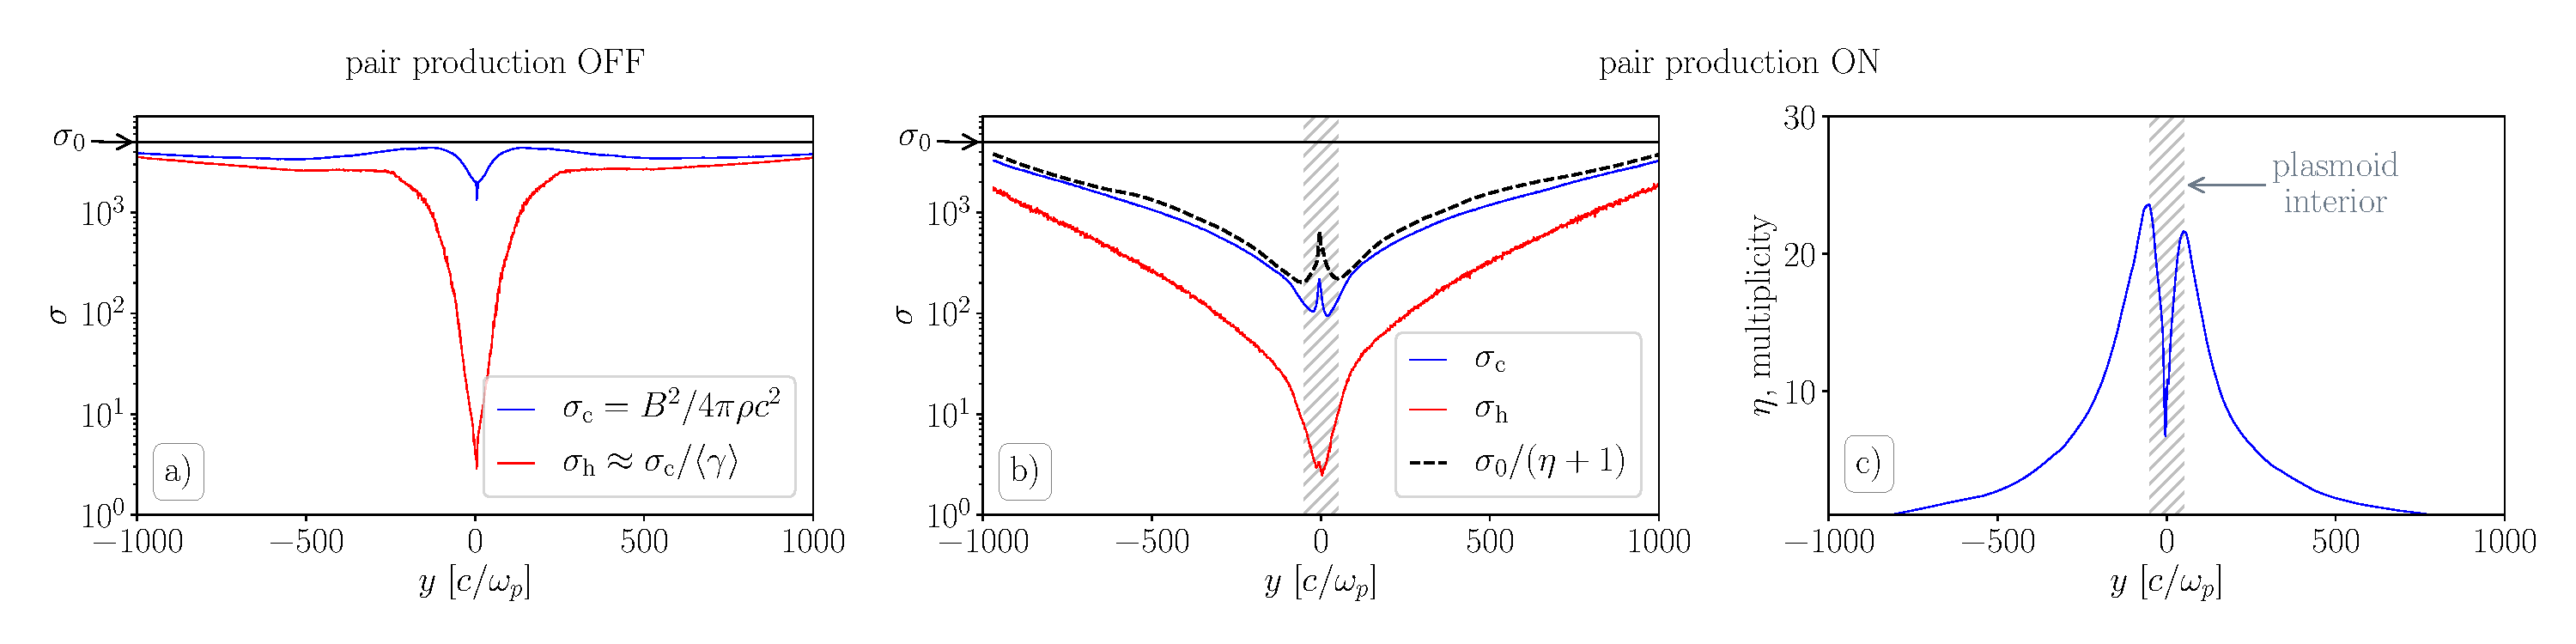
\includegraphics[width=\textwidth]{figures/ch4-pairproduction/fig7.pdf}}
    \caption{Cold magnetization parameter, $\sigma_{\rm c}=B^2/4\pi\rho c^2$, and hot magnetization parameter, $\sigma_{\rm h}=B^2/4\pi\langle\gamma\rangle\rho c^2$, averaged along the current sheet and over time for the runs without (a) and with pair production (b). Panel (c) shows the average multiplicity (density of secondary pairs divided by the density of primary pairs). Shaded regions show the interior of plasmoids where the multiplicity is suppressed artificially. Two solid black lines show the level of the upstream magnetization $\sigma_{\rm c}$, which, when divided by multiplicity, gives the effective magnetization (black dashed line). In contrast to the case without pair production (a), when secondary plasma is produced the magnetization is reduced by a factor of multiplicity (b). Also, since the newly born pairs are hot, $\sigma_{\rm h}$ is also reduced in the upstream.}
    \label{fig:pairprod-sigmas_cut}
\end{figure}

% The plasmoids, on the other hand, are much colder than in case when there is no pair production. This is because the mass loading by secondary plasma decreases the available magnetic energy budget per particle, dropping the effective magnetization by a factor of the multiplicity, $\sigma_{\rm eff}<\sigma_0$.

Pair production also decreases the effective magnetization. To demonstrate this effect, in Figure~\ref{fig:pairprod-sigmas_cut} we plot the cold, $\sigma_{\rm c}\equiv B^2/4\pi\rho c^2$, and hot, $\sigma_{\rm h}=\sigma_{\rm c}/\langle\gamma\rangle$, magnetization parameters, as well as the multiplicity of the secondary plasma, averaged along the $x$-axis and plotted against the $y$-axis.  Fig.~\ref{fig:pairprod-sigmas_cut}a is the fiducial run without pair production or cooling, while Fig.~\ref{fig:pairprod-sigmas_cut}b,c are for the run with pair production.

In Fig.~\ref{fig:pairprod-sigmas_cut}a we see that the cold magnetization parameter is very close to the far upstream value, $\sigma_0$, shown with a black solid line. On the other hand, pair production suppresses this number (Fig.~\ref{fig:pairprod-sigmas_cut}b) by a factor of $\eta +1$, where $\eta$ is the effective multiplicity, also computed {\it in situ} (see Fig.~\ref{fig:pairprod-sigmas_cut}c).\footnote{The local multiplicity here is defined as the density of secondary pairs produced via two-photon pair production divided by the density of primary pairs originally injected from the boundaries.} Note also that the hot magnetization, $\sigma_{\rm h}$ (red line), in the case with pair production, differs strongly from $\sigma_{\rm c}$ (blue line) even in the upstream. This underscores the fact that the upstream plasma, which is dominated by secondary pairs, is hot.

Pair production also has a strong impact on the overall dynamics and evolution of plasmoids. Figure~\ref{fig:snapshot} shows a typical snapshot from one of our pair producing simulations with higher $\sigma_0$. In this figure we show the plasma density (Fig.~\ref{fig:snapshot}a), the density of high energy photons with $h\nu>50$ MeV (Fig.~\ref{fig:snapshot}b) and the local multiplicity (Fig.~\ref{fig:snapshot}c).
% When there is no pair production, plasmoids can grow only through the slow accretion of plasma from the upstream region and through plasmoid mergers. However, when pair production is present the steady state multiplicities reached in our simulations are as high as a few hundred, at which point the whole dynamics of reconnection is controlled by hot secondary pairs, injected by the pair production in the upstream. Plasma accretion onto plasmoids is thus more aggressive with pair production; plasmoids are constantly fed by this secondary plasma, which is then accumulated around the plasmoids in concentric layers that mark the age of the plasmoid (very similar to growth rings in trees, see panel A and C in Fig.~\ref{fig:snapshot}).
Without pair production the plasmoids can grow only through the slow accretion of plasma from upstream and through plasmoid mergers. When pair production is enabled, plasmoids radiate high energy photons (Fig.~\ref{fig:snapshot}b), some of which can pair produce with the low energy photons near the plasmoid peripheries (see high multiplicity regions in Fig.~\ref{fig:snapshot}c). This additional mass loading with hot secondary plasma produces more radiation that pair produces further, and the plasmoid continues to expand as it is being advected out of the simulation box.

In the real reconnection this plasmoid growth will cease once the emitted photons can no longer pair produce near plasmoid peripheries. This can happen either because the optical depth across the plasmoid is large and the photons never escape from it, or because the plasmoid cools down, and the radiated photons have energies that are too low. In our simulations we allow these high energy photons to escape from the plasmoids before they pair produce.

In addition, the mergers constantly eject new high energy photons from freshly accelerated particles. These photons can then pair produce outside the current sheet, providing even more secondary plasma to the plasmoids. Because of this, plasmoids are typically larger and slower for higher multiplicities. When the sizes of plasmoids become comparable to the simulation box size, they effectively slow down the reconnection rate and in some situations can nearly stop it. After plasmoids leave the simulation box, the reconnection continues with the regular rate at $\beta_{\rm in}\approx 0.1\text{-}0.2$. The movie of our simulation from Fig.~\ref{fig:snapshot} that shows a large plasmoid and explosive photon ejections during plasmoid mergers is available \href{\linkVidOne}{online}.\footnote{Direct link: \url{\linkVidOne}.}

% Ultimately, it is clear that the macroscopic properties of the steady state, such as the formation and growth of plasmoids, their dynamics and pressure support, are different depending on whether there is synchrotron cooling or pair production in the system.
% \sasha{whant to comment how particles are accelerated in mergers in the case of strong cooling?};\hayk{I don't understand this}

\begin{figure}[H]
    \centering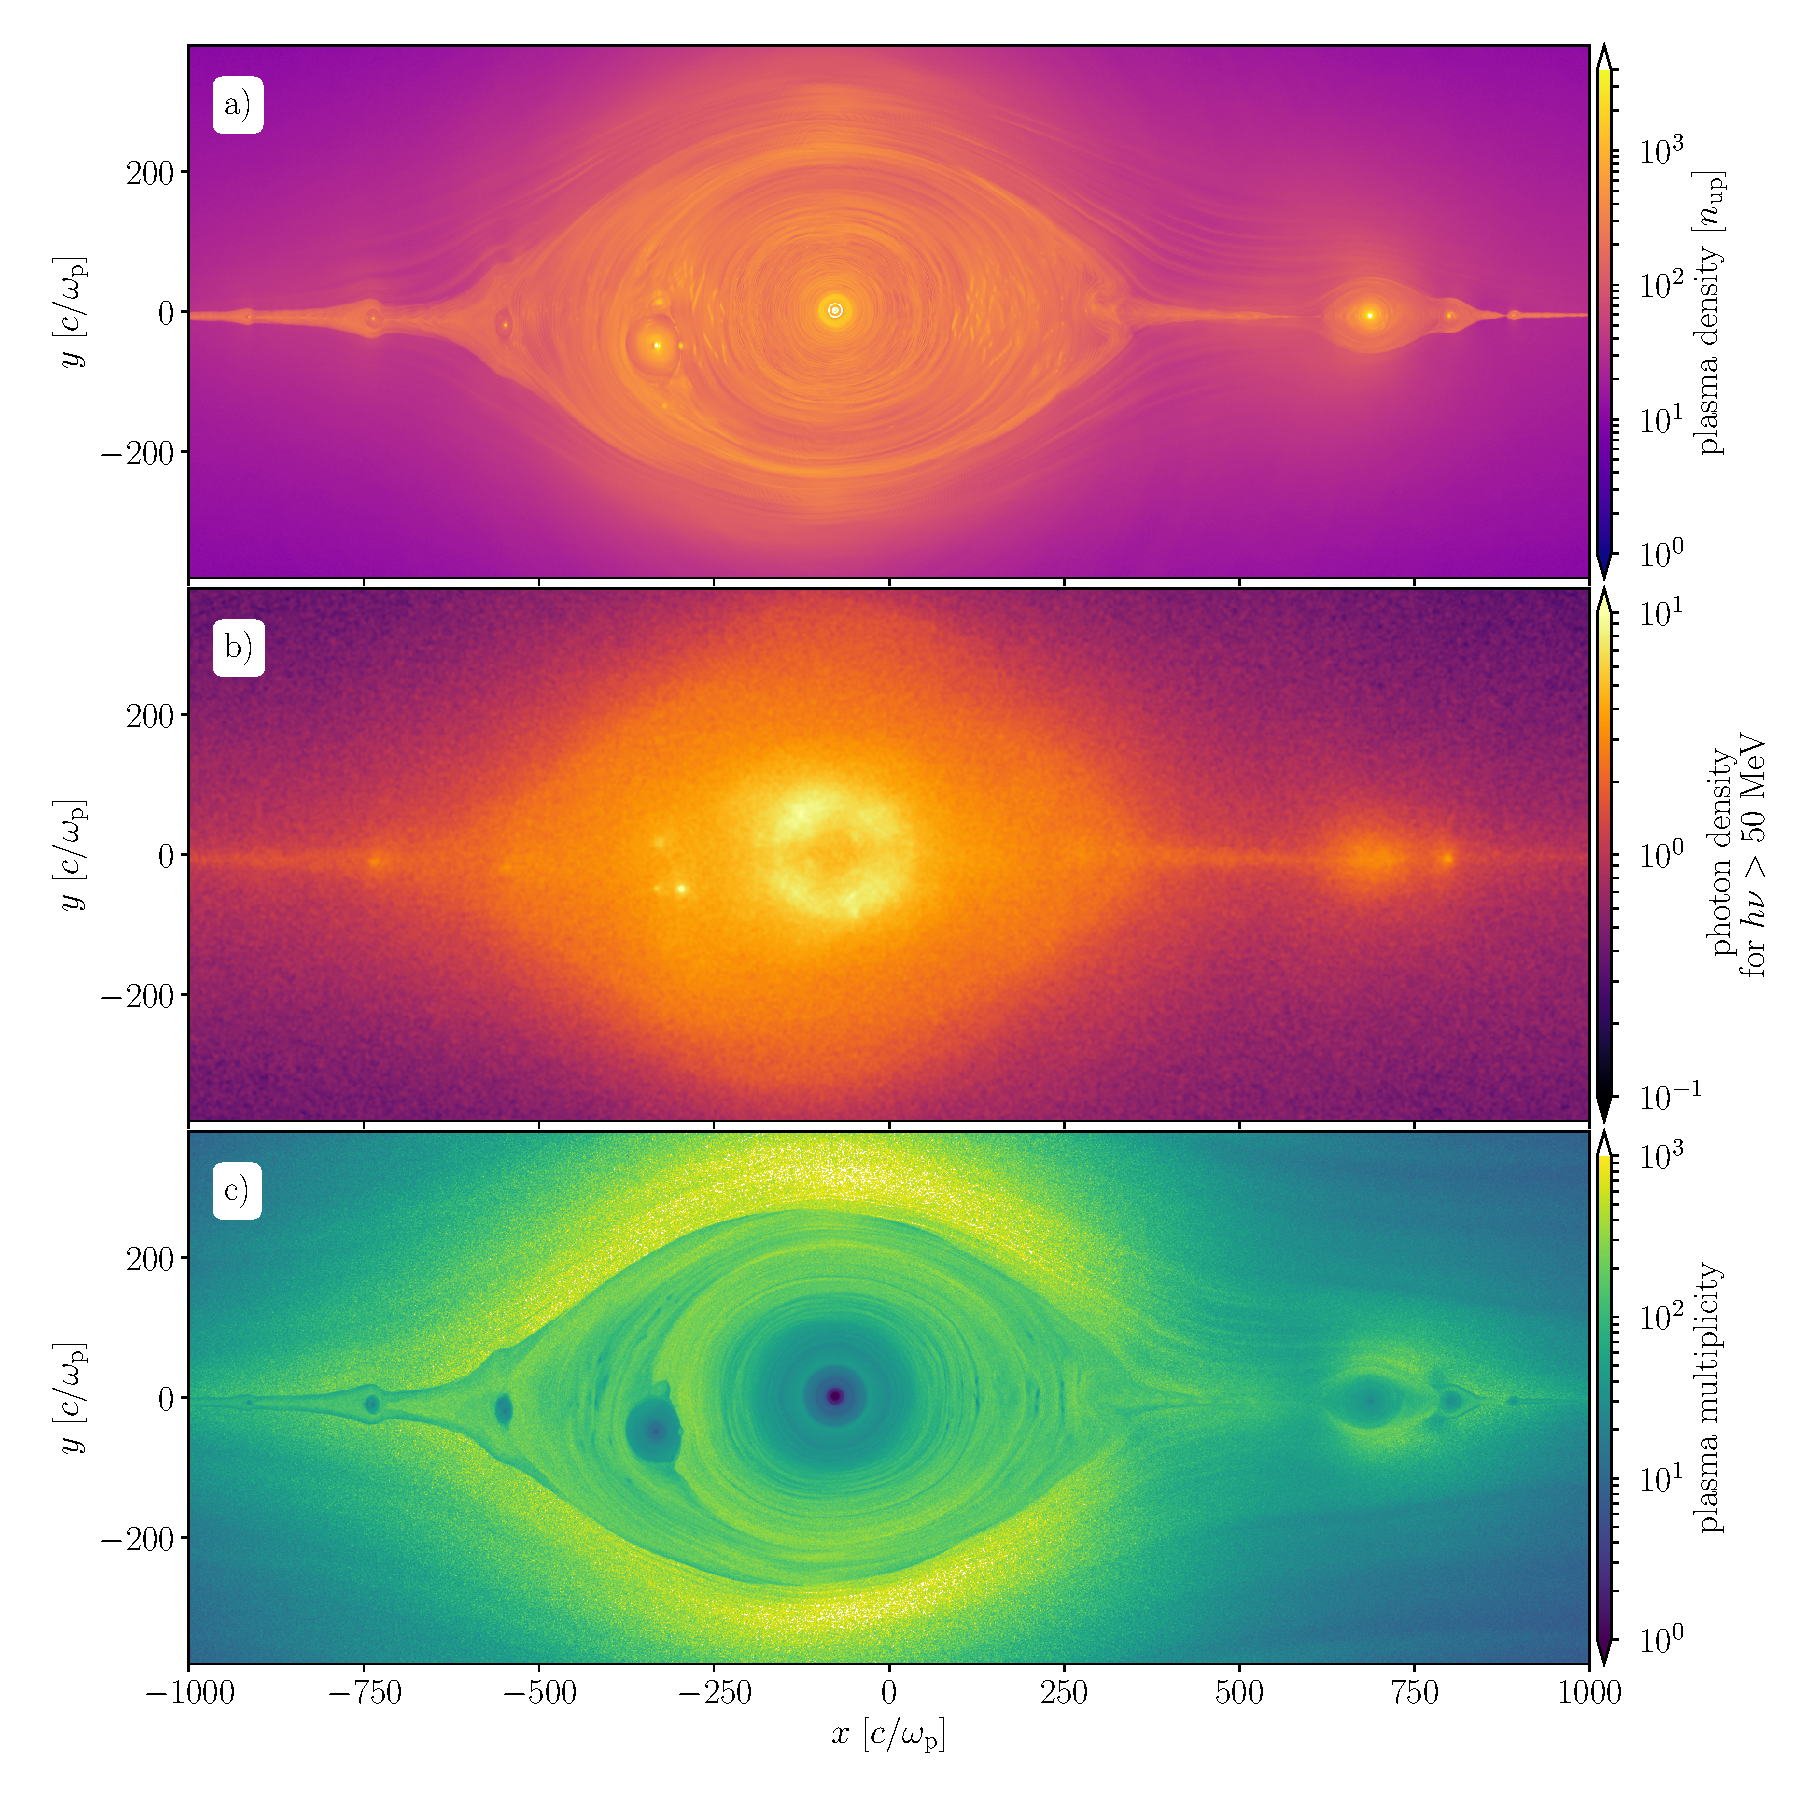
\includegraphics[width=0.9\textwidth]{figures/ch4-pairproduction/fig8.pdf}
    \caption{Snapshot from a simulation of the reconnection with the cooling and pair production with $\sigma_0=10^4$, $\gamma_c=50$, $\gamma_{\rm rad}=1000$, $p_0=10^{-5}$. The box extends further in the vertical direction, in this figure we focus on the large plasmoid. Plots show (a) the total plasma density normalized by the initial upstream density, (b) the density of photons with $h\nu>50$ MeV, (c) the local plasma multiplicity, $\eta$, defined as the density of secondary plasma divided by the density of the injected plasma. Interiors of plasmoids are low in multiplicity since we allow photons to escape from them without having a chance to pair produce. Maximum density in the top plot (in white) indicates the region, where we turn off cooling to prevent plasmoids from getting too dense and making the local skin depth unresolved. When the pair production is enabled the upstream is abundant with secondary plasma and also plasmoids are typically larger and slower, since they rapidly expand via pair production. In this snapshot the massive plasmoid in the middle is undergoing mergers with smaller plasmoids, one of which (at $x=-300$, $y=-50$) has not yet been fully absorbed. Most of the photons are emitted within plasmoids close to their centers, where both the magnetic field and density are high. Lack of high energy photons in the very middle of the large plasmoid is due to the fact that plasma in that region is cold. The full movie of this simulation is available \href{\linkVidOne}{online} (direct link: \url{\linkVidOne}).}
    \label{fig:snapshot}
\end{figure}

\subsection*{Particle acceleration and the emerging radiation spectra}
\label{sec:pairprodaccell}

\begin{figure}[htb]
    \centering
    \centerline{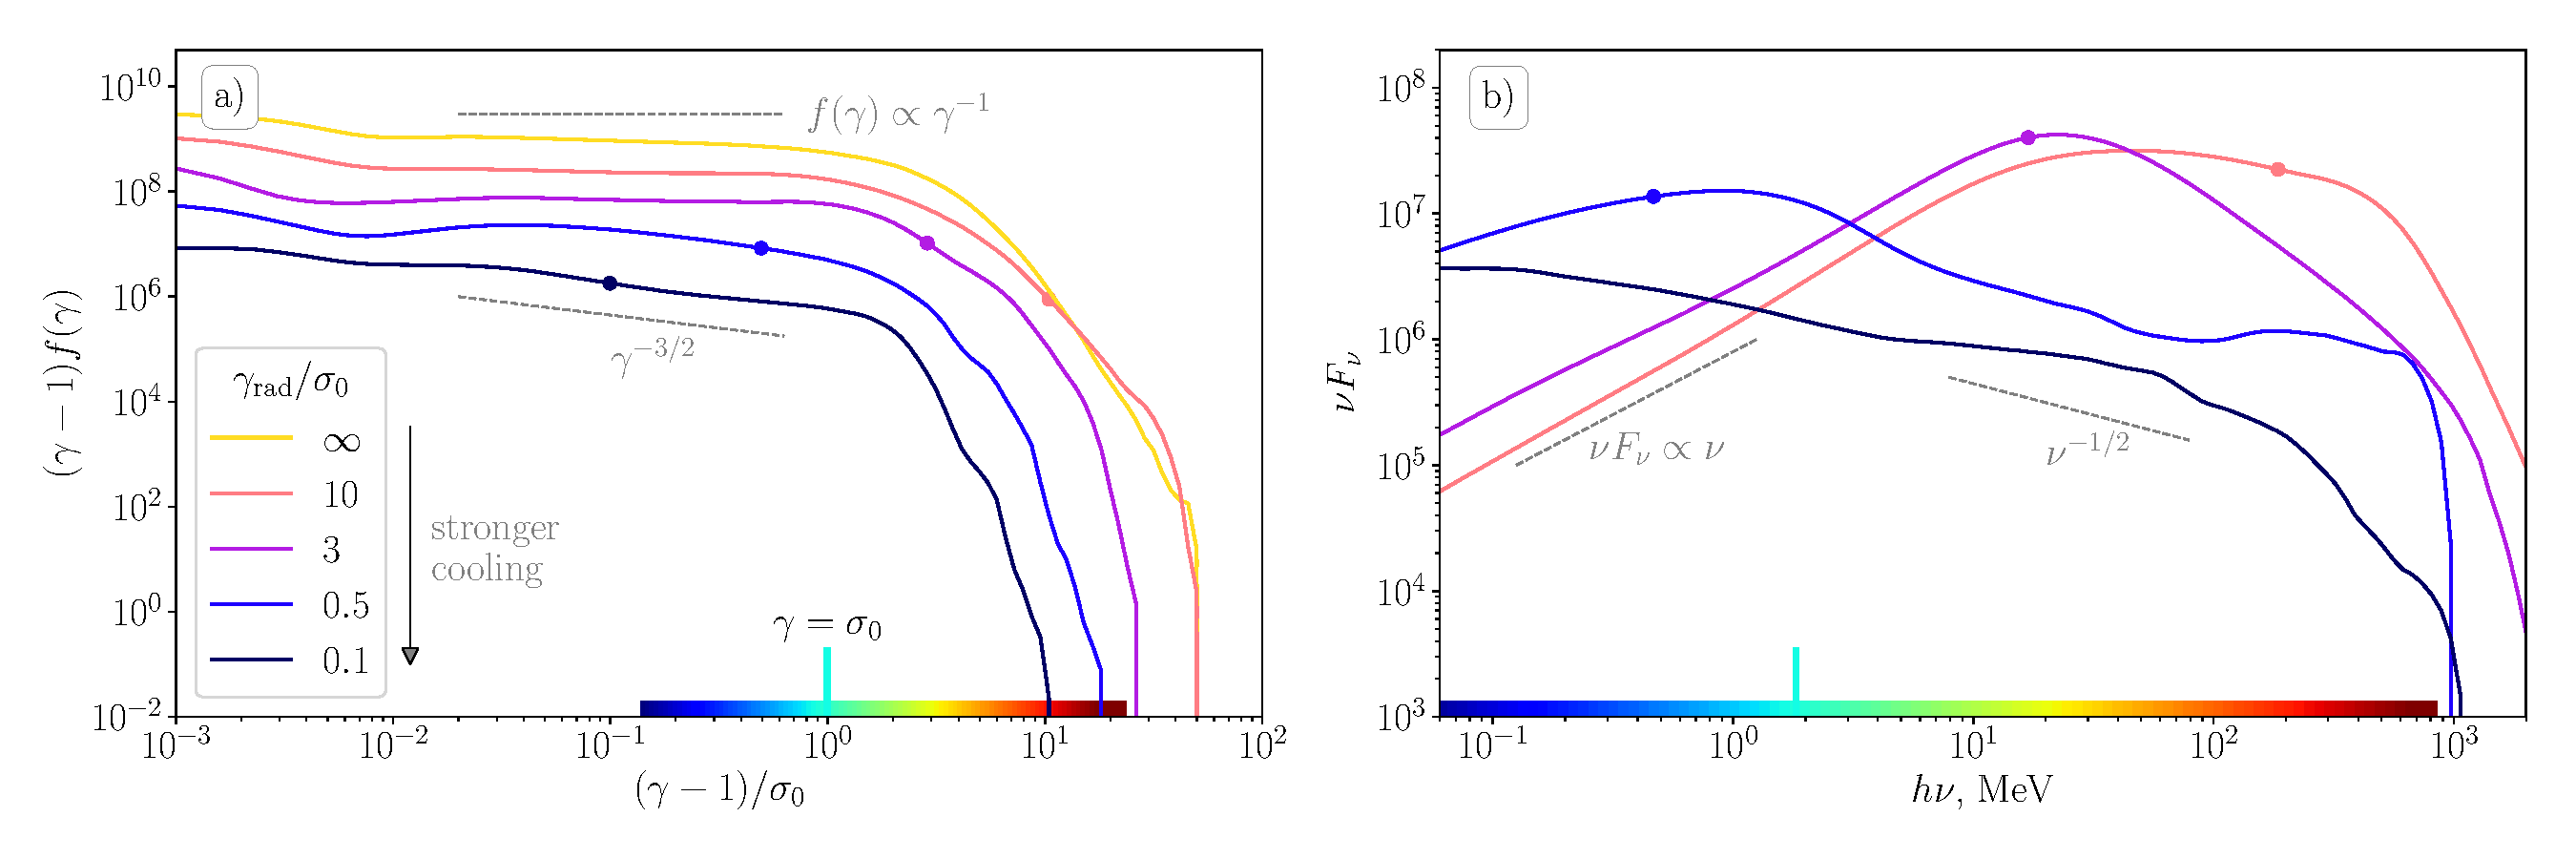
\includegraphics[width=\textwidth]{figures/ch4-pairproduction/fig9.pdf}}
    \caption{Particle and photon spectra for the $\sigma_0=200$ simulations without pair production for different cooling regimes in late-time steady state. The cooling decreases, i.e., $\gamma_{\rm rad}$ increases, from dark blue to yellow; $\gamma_{\rm rad}=\infty$ is the case without cooling (i.e., no photons). Two colorbars below put particle energies and synchrotron photon energies into correspondence, given a fixed background magnetic field, which in general varies depending on particle position. Particle spectra are shifted vertically for illustration purposes; circles indicate $\gamma_{\rm rad}$ for each case as well as the corresponding synchrotron photon energy in the upstream magnetic field. Cooling typically conserves the $\gamma^{-1}\text{-}\gamma^{-3/2}$ slope of the particle energy distribution function. Peaks in synchrotron photon spectra for each case corresponding to $\gamma_{\rm rad}$ in particles; high energy tails with $\nu F_{\nu}\propto \nu^{-1/2}$ are formed during transient mergers, when particles accelerated in secondary current sheets are captured by plasmoids and rapidly cooled.}
    \label{fig:pairprod-no_pair_runs}
\end{figure}

We now focus on how cooling and pair production affect particle acceleration in reconnection, and how the resulting particle and photon spectra are formed. To distinguish the effects of cooling and pair production we first analyze the process without pair production. We test how the cooling regime affects particle and radiated photon spectra (cf., e.g., \citealt{2016ApJ...833..155K, 2018JPlPh..84c7501N}).

The cooling regime is characterized by the ratio $\gamma_{\rm rad}/\sigma_0$, which effectively sets the cooling time compared to the acceleration time $\sim (t_{\rm cool}/t_{\rm acc})^{1/2}$. If this ratio is $\gg 1$, the cooling is inefficient, i.e., the cooling time is much longer than the acceleration time, and vice versa. Note, however, that this ratio is defined for the upstream magnetic field, so the actual cooling time of a particle will depend on the local magnetic field.

We initialize our simulations with the magnetization parameter $\sigma_0=200$ and cold plasma in the upstream. We fix $\gamma_c=50$ and vary $\gamma_{\rm rad}$ to study the different regimes. The results of our runs are shown in Figure~\ref{fig:pairprod-no_pair_runs}, where we plot the particle and photon spectra (computed for the whole simulation domain) for the runs in different cooling regimes: from no cooling (yellow line) to strong cooling (dark blue line). The horizontal colorbar puts into correspondence the particle energies and the energies of synchrotron photons that would have been radiated by these particles in the upstream magnetic field; circles on the lines mark $\gamma_{\rm rad}$ and the corresponding synchrotron photon energy.

When the cooling is weak, $\gamma_{\rm rad}/\sigma_0\gg 1$, particles form a power-law, $f(\gamma) \propto \gamma^{-1}$, similar to what is observed in uncooled simulations for high $\sigma_0$ (cf., e.g., \citealt{2014ApJ...783L..21S}). The strong cooling cases have slightly steeper spectra (close to $f(\gamma)\propto \gamma^{-3/2}$). For all values of $\gamma_{\rm rad}$ the power-law slope is followed by a steep decay at higher energies (close to a few times $\sigma_0$, see Fig.~\ref{fig:pairprod-no_pair_runs}a).

The overall picture is then as follows: particles are accelerated in primary and secondary current sheets up to a few times $\sigma_0 m_e c^2$. The magnetic field in these current sheets is weak, and the cooling time, $t_{\rm cool}$, is much longer than the residence time in the x-points. This means that the cooling is inefficient close to the current sheets, and the particles remain hot until they are captured by the plasmoids, where they cool down to energies $<\gamma_{\rm rad}$. Since the acceleration and cooling happen in different regions, we do not expect a different power-law slope or any pronounced power-law break in the particle distribution function close to $\gamma_{\rm rad}$. The cutoff energy in particles is dictated by the acceleration in x-points, and is typically a few times $\sigma_0$. Note that there is no growth of this cutoff over time due to plasmoid compression as found in the uncooled simulations of \cite{2018arXiv180800966P}, because particles within the plasmoids are efficiently cooled to $\gamma_{\rm rad}$ in our runs, unless the cooling is too weak $\gamma_{\rm rad}/\sigma_0\gg 1$.

The corresponding time-averaged photon spectra are shown in Fig.~\ref{fig:pairprod-no_pair_runs}b. A standard result in the theory of synchrotron radiation is that particles constantly injected with a power-law energy distribution $f(\gamma)\propto \gamma^{-p}$ form a synchrotron spectrum described as $\nu F_{\nu}\propto \nu^{-(p-3)/2}$ \citep{1979rpa..book.....R}. In our simulations, the plasma that resides within the plasmoids ($\gamma < \gamma_{\rm rad}$)  and forms a power-law spectrum with $p\approx 1$, radiates $\nu F_{\nu}\propto \nu$ synchrotron spectrum (see photon spectra before the peak in Fig.~\ref{fig:pairprod-no_pair_runs}b). The peaks in photon spectra correspond to particles with the energy $\gamma_{\rm rad}$ radiating in magnetic fields of value close to the upstream field.

Photons with energies beyond the peak frequency are radiated by the particles with energies up to a few times $\sigma_0$. These particles enter the plasmoids after being accelerated in x-points and rapidly lose their energy, being exposed to a large perpendicular magnetic field, until they cool down to $\gamma\lesssim \gamma_{\rm rad}$. As a result, the photon spectrum at high energies is highly fluctuating in time, since there is no steady population of high energy particles ($\gamma > \gamma_{\rm rad}$) in a large magnetic field. The majority of these high energy photons, especially for the strong cooling regime ($\gamma_{\rm rad}/\sigma_0\ll 1$), are radiated during violent events such as plasmoid mergers. Averaged over time,  these transients form an extended power law tail (close to $\nu^{-1/2}$). We also present these results in the form of movies to better illustrate how the transients work both in \href{\linkVidThree}{strong} and \href{\linkVidTwo}{weak} cooling regimes.\footnote{Direct links: \url{\linkVidThree} and \url{\linkVidTwo}.}.

Further, we discuss the results of our runs with pair production. For all the runs below we chose the parameters to be $\sigma_0=10^3\text~\text{to}~4\times10^4$, $\gamma_{\rm rad} = 10^3$, $\gamma_c=50$ and $p_0=10^{-5}$. These values are chosen to satisfy the relation $\gamma_c \ll \gamma_{\rm rad} \lesssim \sigma_{\rm eff}$. We also want the synchrotron peak to be roughly at $0.1\text{-}1$ GeV, which fixes $\gamma_c$ and $\gamma_{\rm rad}$. %Cross section magnitude, $p_0$, is chosen in such a way that for the photons of all energies the optical depth to pair production is $<1$ (see more on that in the appendix~\ref{sec:appendixA}).

\begin{figure}[htb]
    \centering
    \centerline{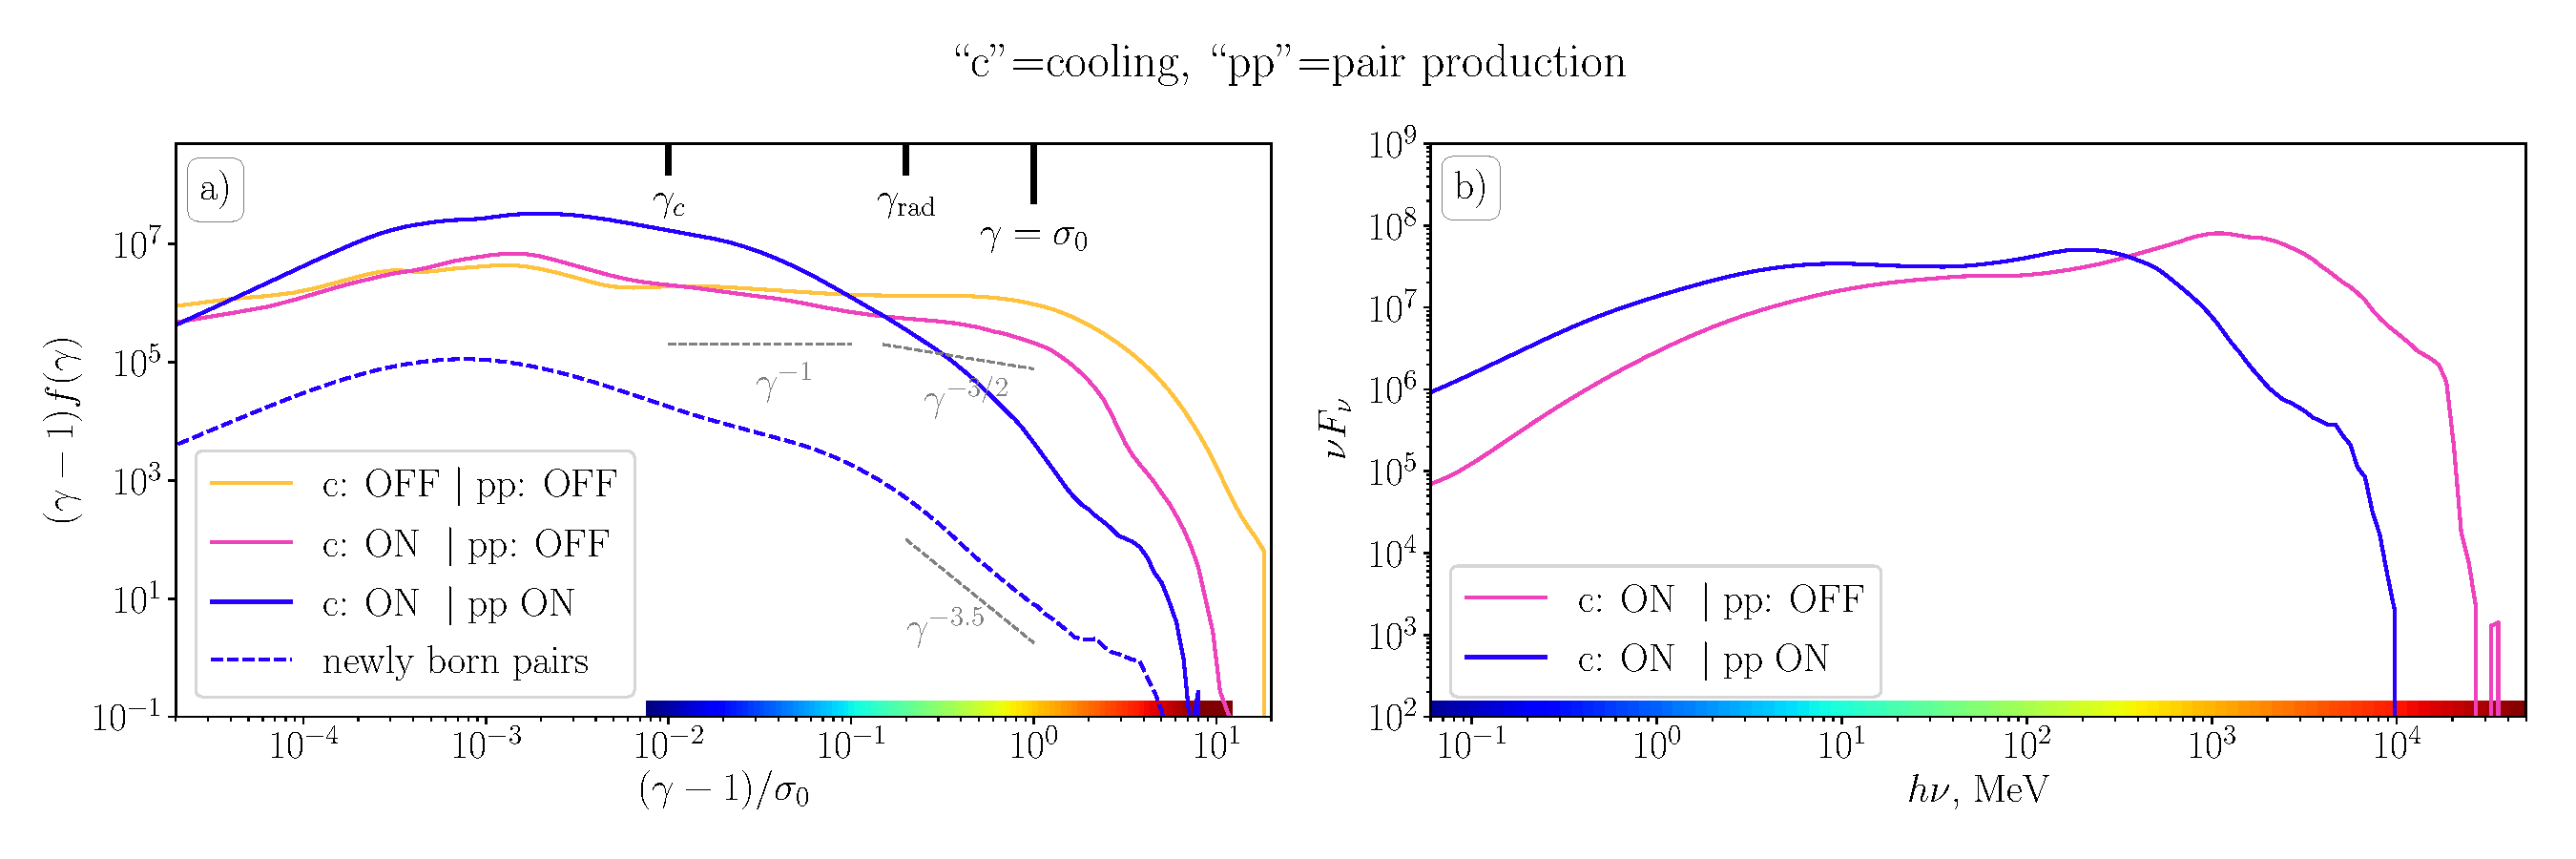
\includegraphics[width=\textwidth]{figures/ch4-pairproduction/fig10.pdf}}
    \caption{Particle (a) and photon (b) spectra for the $\sigma_0=5000$, $\gamma_{\rm rad} = 1000$, $\gamma_c=50$ simulations without cooling, with cooling but without pair production, and with both cooling and pair production enabled in late-time steady state. Two colorbars below put particle energies and synchrotron photon energies into correspondence, given a fixed background magnetic field. Dashed line is the spectrum of newly born secondary pairs in the run with pair production. Cooling does not strongly affect the slope, whereas when pair production is enabled the effective magnetization is dropped, and the upstream is no longer cold (see the newly born pairs). This causes the shift of the peak in photon spectrum (corresponding to the effective magnetization, $\sigma_{\rm eff}$).}
    \label{fig:pairprod-pair_runs}
\end{figure}

We first focus on a single value of $\sigma_0=5000$ to see how enabling pair production changes the shape of the particle and photon spectra. In Figure~\ref{fig:pairprod-pair_runs} we present the energy distribution of particles (Fig.~\ref{fig:pairprod-pair_runs}a) and photons (Fig.~\ref{fig:pairprod-pair_runs}b) for three runs: without cooling or pair production (yellow line), with cooling but without pair production (pink line), and with both cooling and pair production (blue line).

Cooling without pair production does not strongly affect the particle spectrum of $f(\gamma)\propto \gamma^{-1}\text{-}\gamma^{-3/2}$, in agreement with what we found earlier, only slightly decreasing the energy cutoff (see yellow and pink lines in Fig.~\ref{fig:pairprod-pair_runs}a). On the other hand, when pair production is on, the spectrum is no longer flat and there is no clear cutoff energy. Instead, particles form a wide power-law distribution, ranging from $\gamma^{-2}$ to $\gamma^{-4}$.

There are two effects causing this. First, since the layer is being mass loaded with secondary plasma, the effective magnetization parameter, $\sigma_{\rm eff}$, decreases compared to the upstream magnetization, $\sigma_0$. This means that the reconnection has less magnetic energy per particle and the resulting spectrum shifts to lower energies. At the same time, the newly born secondary pairs (dashed blue line in Fig.~\ref{fig:pairprod-pair_runs}a) that have not yet been accelerated in the electric field at the x-point, form a steep power law with $f(\gamma)\propto \gamma^{-3}\text{-}\gamma^{-4}$ up to the highest energies. This means that, unlike two other cases where the current sheet was being fed by an initially cold plasma, in this case the upstream secondary plasma is already hot, due to a wide distribution in energies of parent photons that produced these pairs.

This behavior is also reflected in the photon spectrum (Fig.~\ref{fig:pairprod-pair_runs}b), where the peak is shifted due to the reduced magnetization. The peak in photons corresponds to $\gamma\approx \sigma$ in particles, where in the case of pair production the value of $\sigma$ is reduced with respect to $\sigma_0$ by a factor of multiplicity. In this particular run, presented in Fig.~\ref{fig:pairprod-pair_runs}, the multiplicity is of the order of a few, and thus the effective magnetization is few times less than $\sigma_0$. The resulting peak frequency is proportional to the particle energy squared, and is, therefore, smaller by roughly an order of magnitude.

\begin{figure}[htb]
    \centering
    \centerline{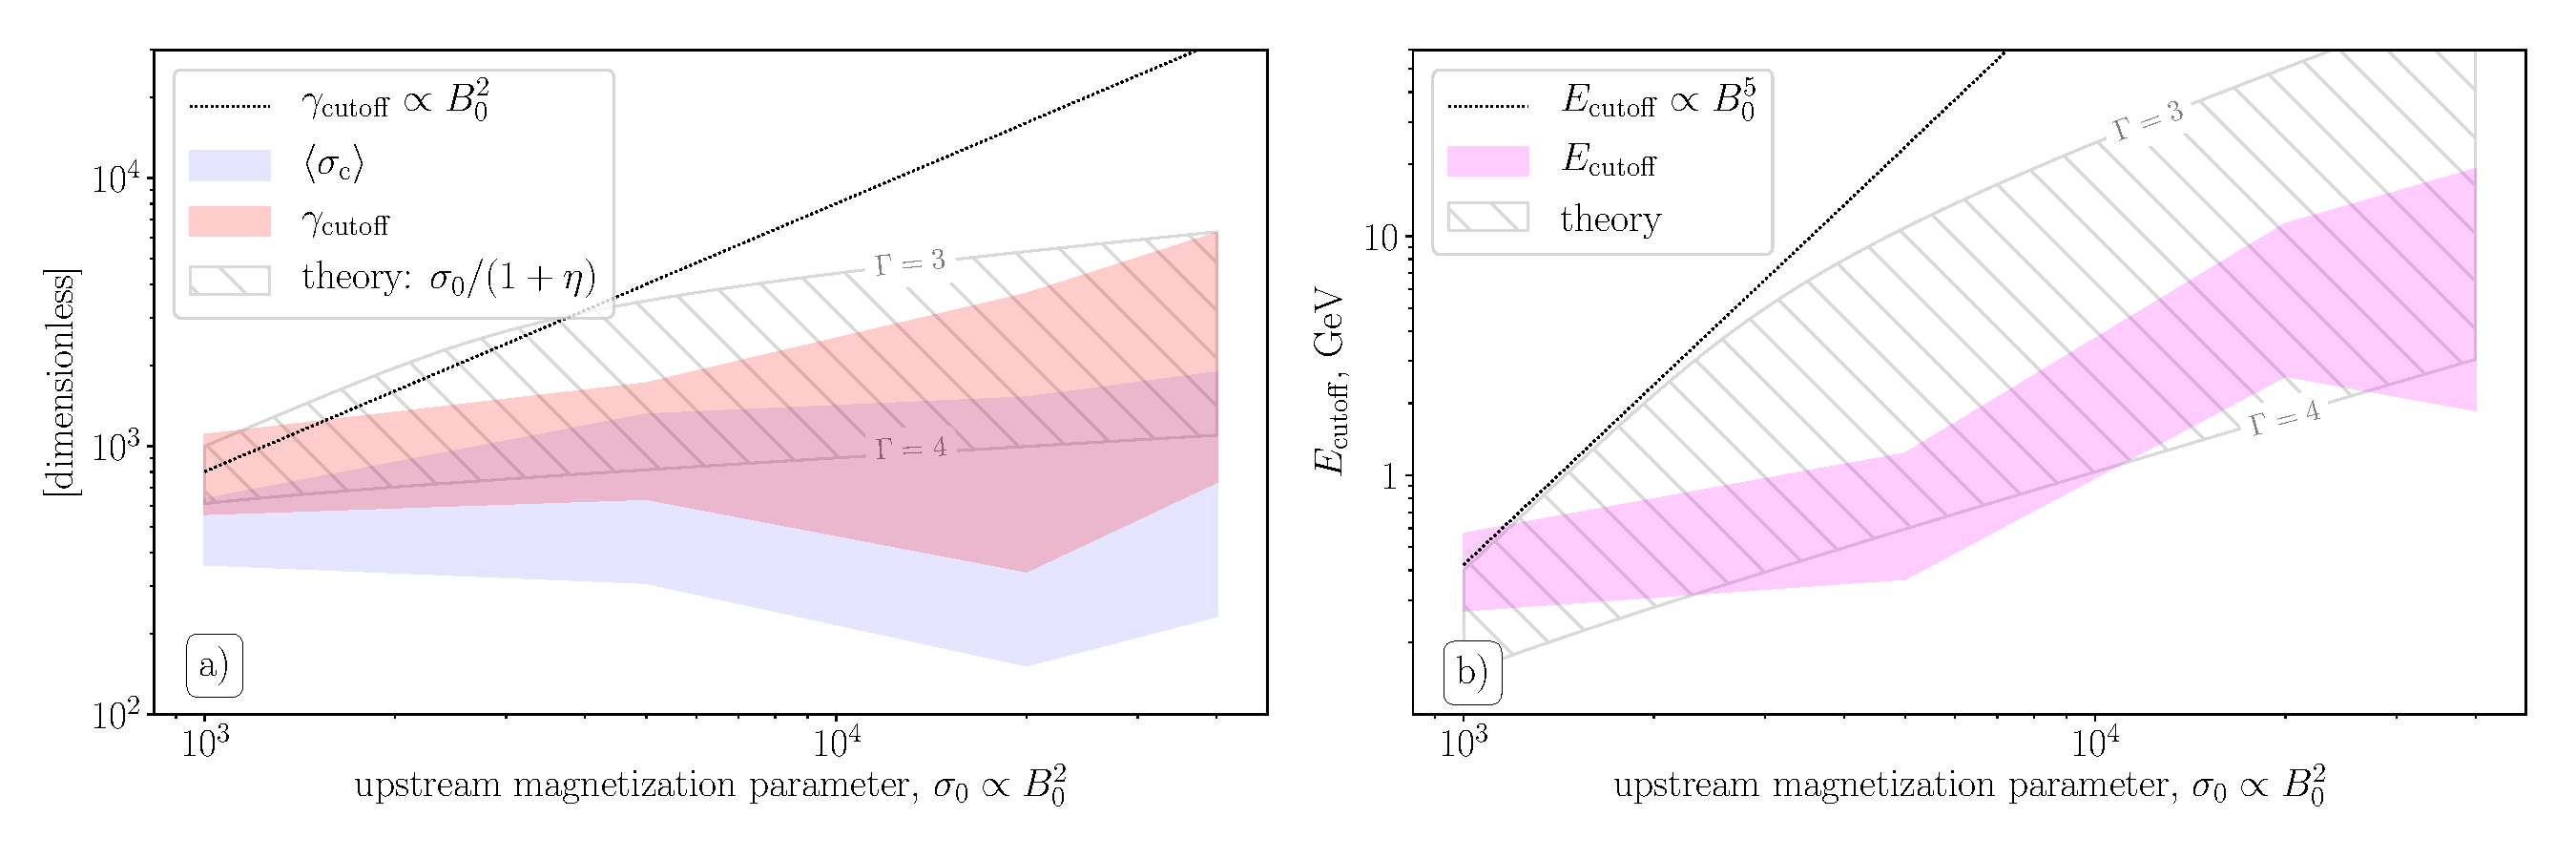
\includegraphics[width=\textwidth]{figures/ch4-pairproduction/fig11.pdf}}
    \caption{Box-averaged quantities from four of our simulations: (a) magnetization $\langle\sigma_{\rm c}\rangle$ (blue) and particle spectra cutoff $\gamma_{\rm cutoff}$ (red); (b) photon spectral cutoff $E_{\rm cutoff}$ (magenta), all plotted against the initial magnetization parameter, $\sigma_0$, which is proportional to the background magnetic field squared, $B_0^2$. Widths of the colored regions represent the uncertainties in determining these parameters from simulations. Dotted black lines are simple scalings without pair production feedback, and hatched regions are theoretical predictions with photon indexes $\Gamma=3\text{-}4$.}
    \label{fig:pairprod-cutoffs_vs_sigma}
\end{figure}

Finally, in Figure~\ref{fig:pairprod-cutoffs_vs_sigma} we show how the particle cutoff, box averaged $\sigma_{\rm c}$ (defined similar to Fig.~\ref{fig:pairprod-sigmas_cut}b) and spectral cutoff for photons depend on $\sigma_0$, i.e., the background magnetic field $B_0$ (since $\sigma_0\propto B_0^2$ for fixed density). The average cold magnetization, $\langle \sigma_{\rm c}\rangle$ (blue line in Fig.~\ref{fig:pairprod-cutoffs_vs_sigma}a), is found by averaging $B^2/4\pi\rho c^2$ over a region around the current sheet where most of the pair production takes place. Different sizes of this region give different values, which we represent as errorbars. To determine the cutoffs we define a model-independent measure of how far our spectrum extends
\begin{equation}
    \gamma_{\rm cutoff}\sim \frac{\int\mathrm{d}\gamma f(\gamma)\gamma^\alpha}{\int\mathrm{d}\gamma f(\gamma)\gamma^{\alpha-1}},
\end{equation}
and the same for photons (similar to what was done by~\citealt{2015ApJ...809...55B}). This gives a rough estimate of where the spectral break (or the cutoff) is. Power $\alpha$ is empirically chosen to be between $2$ and $3$: varying $\alpha$ in that range gives different cutoff energies which we present as errorbars (as a rough estimate of how wide and uncertain the cutoff is).

We compare our findings with the simple predictions without pair production feedback:
\begin{equation}
    \gamma_{\rm cuttoff}\propto \sigma_0\propto B_0^2,~~~E_{\rm cutoff}\propto \gamma_{\rm cuttoff}^2 B_0\propto B_0^5,
\end{equation}
and also overplot the predicted effective magnetization, $\sigma=\sigma_0 / (1+\eta)$, and the corresponding synchrotron cutoff energies (hatched regions in both plots). For that, we estimate the steady state multiplicity (see equation~\ref{eq:pairprod-sim_mult_theory}) with different values of the photon power law index $\Gamma$.

First, note that both the cutoff energy and the magnetization are reduced compared to simple predictions without pair production feedback. This means that not only is the maximum energy of particles lower with pair production, but there is an effective upstream magnetization, $\sigma_{\rm eff}$, that is decreased from the initial value $\sigma_0$ by a factor of multiplicity of secondary plasma.

From the runs with different values of $\sigma_0$ we find that the particle cutoff, $\gamma_{\rm cutoff}$, grows roughly as $B_0^{0.2\text{-}0.5}$ with the background magnetic field, and the photon spectral cutoff energy, $E_{\rm cutoff}$, grows as $B_0^{1.2\text{-}1.8}$. These two scalings are consistent with each other, since $E_{\rm cutoff}\propto \gamma_{\rm cutoff}^2 B_0$. We can compare these results with simple predictions described by equation (\ref{eq:pairprod-sim_mult_theory}). In our simulations the distribution function of high energy photons has a power law index $\Gamma\approx 3\text{-}4$ (corresponding to spectral index $\nu F_{\nu}\propto \nu^{-1}\text{-}\nu^{-2}$). To zeroth order, scale lengths $s_1$ and $s_2$ from  (\ref{eq:pairprod-sim_mult_theory}) can be taken to be equal to the size of the simulation box $L$. In these simulations we have $L / \sigma \rho_0 \approx 70 (\sigma_0 / 10^3)^{-1/2}$, since the box has a fixed number of cells, but the gyroradius scales with the upstream magnetization. With $s_1 = s_2 = L$ and $\eta \gg 1$, we get roughly $\eta \propto \sigma_0$, meaning that the effective magnetization scales weakly with $\sigma_0$: $\sigma = \sigma_0 / (1+\eta) \approx const$ and $E_{\rm cutoff}\propto B_0$.
Taking $f_0\approx 0.1\text{-}0.01$, $\beta_{\rm rec}\approx 0.1$, $\gamma_c = 50$, $\gamma_{\rm rad} = 1000$, and $\Gamma=3\text{-}4$, we find that the steady state multiplicity for $\sigma_0=10^4$ is $\eta\approx 2\text{-}10$, while for $\sigma_0 = 4\times 10^4$ it is $\eta\approx 10\text{-}50$, which roughly agrees with what we see. However, as our simplified model does not account for time variability, we underestimate the multiplicity by a factor of a few, which results in a slightly higher effective magnetization (compared to $\langle\sigma_{\rm c}\rangle$).
%Presumably\hayk{a better word here}, a factor of a few is not crucial, %given that the model is very naive and does not account for the time %variability of the system and other possible complications.

To interpret these results in terms of observations, one should note that in these simulations we only varied the background magnetic field, while keeping the upstream plasma density constant. However, in reality the inflowing plasma density from the inner magnetosphere to the Y-point depends also on the magnetic field and period of the pulsar, as the overall plasma density is normalized by Goldreich-Julian density $n_{\rm GJ}=\bm{\Omega}\cdot\bm{B}/2\pi ce$. This will further make the dependence of cutoff energy on the magnetic field at the light cylinder even weaker.

\begin{figure}[htb]
    \sidebysidecaption{0.555\linewidth}{0.42\linewidth}{
        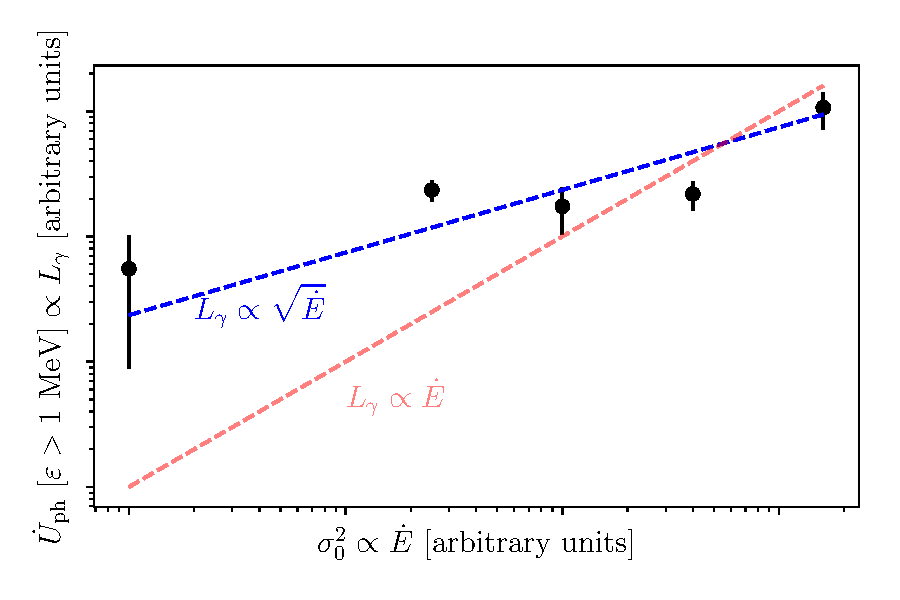
\includegraphics[width=\textwidth]{figures/ch4-pairproduction/fig12.pdf}
    }{
        \caption{High energy photon luminosity in our simulations plotted against the square of the initial upstream magnetization, which in pulsars should be proportional to the Poynting flux and thus the spin-down rate $\dot{E}$. The observed $L_\gamma\propto\sqrt{\dot{E}}$ (in blue) and expected $L_\gamma\propto\dot{E}$ (if no pair production were present, in red) trends are also shown.}
        \label{fig:pairprod-Lgamma_Edot}
    }
\end{figure}

Another important observation in $\gamma$-ray pulsars is the dependence of the luminosity in $\gamma$-rays, $L_\gamma$, on the pulsar spin-down rate, $\dot{E}$. For most of the $\gamma$-ray pulsars (with the exception of millisecond pulsars) this dependence is sublinear, with a rough $L_\gamma\propto \sqrt{\dot{E}}$ fit~\citep{2013ApJS..208...17A}. We can evaluate that dependence from our simulations. As $L_\gamma$ we take the energy deposited into the high energy photons ($>$MeV) per unit time. On the other hand, we have the following two relations:
\begin{equation}
    \dot{E}\propto B_{\rm LC}^2 R_{\rm LC}^2,~~~\sigma^{(0)}_{\rm LC}\propto B_{\rm LC}^2 / n_{\rm GJ}\propto B_{\rm LC}R_{\rm LC},
\end{equation}
where we assume that the spin-down energy is carried away in the form of the Poynting flux throughout the light cylinder. Here $\sigma^{(0)}_{\rm LC}$ is the primary magnetization without the feedback from pair production. We thus find that our $\sigma^{(0)}_{\rm LC}\propto B_{\rm LC}R_{\rm LC}$, or $\dot{E}\propto {\sigma^{(0)}_{\rm LC}}^2$, since the spin-down power, $\dot{E}\propto B_{\rm LC}^2 R_{\rm LC}^2$, depends only on magnetization at the light cylinder.\par

Since the photon production is variable in time, we average $L_\gamma$ over a large number of steps and present the time variability as errorbars. The results are shown in Fig.~\ref{fig:pairprod-Lgamma_Edot}, where we also overplot the observed $L_\gamma\propto\sqrt{\dot{E}}$ trend, and the naively expected $L_\gamma\propto\dot{E}$ trend, which would be applicable if no pair formation were present. As seen in the plot the observed dependence can indeed be understood if the pair production regulates the effective magnetization and thus the photon production in the current sheet.

\section{Discussion \& summary}
\label{sec:pairprod-discussion}

%Let us briefly summarize the main results presented above.
In this work we discussed the results of two dimensional particle-in-cell simulations of radiative relativistic reconnection with pair production. We included both synchrotron cooling and two-photon pair production self-consistently by tracking all the radiated photons as separate particles and colliding them with each other. We then separately studied the effects of both cooling and pair production on particle acceleration and the emission signatures of reconnection. Our main findings are summarized below.

\subsection*{\small \it Synchrotron cooling}

\begin{itemize}[leftmargin=*,wide = 0pt]
  \item Particles with energies $\gamma>\gamma_{\rm rad}$ exist near the peripheries of plasmoids or close to the primary or secondary current layers, where cooling is inefficient. Bulk of the particles within the plasmoids have energies $<\gamma_{\rm rad}$.

  While in the case of non-radiative reconnection large plasmoids contain the bulk of the high energy particles (with energies up to a few times $\sigma_{\rm c}m_e c^2$), when synchrotron cooling is enabled these particles can no longer maintain their energies within the plasmoids due to the strong magnetic field. Thus, the particles in plasmoids are cooled to energies $\gamma < \gamma_{\rm rad}$, while the rest of the high energy plasma, $\gamma > \gamma_{\rm rad}$, exists either around the primary and secondary current sheets or in the vicinities of plasmoids, where the magnetic field is weak, and the cooling is inefficient.
\end{itemize}


\begin{itemize}[leftmargin=*,wide = 0pt]
% \setcounter{enumi}{1}
  \item Cooling removes the pressure support for plasmoids against contraction, and plasmoids become effectively compressive with typically smaller sizes and larger overdensities in the centers.
\end{itemize}

\begin{itemize}[leftmargin=*,wide = 0pt]
% \setcounter{enumi}{2}
  \item Weak cooling, $\gamma_{\rm rad}/\sigma_{\rm c}\gg 1$, preserves the hard power-law in particle energy distribution function $f(\gamma)\propto \gamma^{-1}$; in strong cooling regime, $\gamma_{\rm rad}/\sigma_{\rm c}\ll 1$ the slope steepens towards $f(\gamma)\propto \gamma^{-3/2}$.

  Since the acceleration and cooling of the particles take place in different locations (x-points and plasmoids), there is no cooling break near $\gamma_{\rm rad}$ and the power-law slope of the particle spectrum is generally unaffected.
\end{itemize}


\begin{itemize}[leftmargin=*,wide = 0pt]
% \setcounter{enumi}{3}
    \item The high energy cutoff in particle distribution is only slightly shifted towards the lower energies (still being a few times $\sigma_{\rm c}$). Because of that, the corresponding cutoff in photon spectrum is only marginally affected by cooling.

    This maximum energy is roughly unaffected, because the x-points are still able to accelerate particles effectively up to a few times $\sigma_{\rm c} m_e c^2$, as the cooling is inefficient in current sheets. However, once particles are captured by the plasmoids, where the magnetic field is high, and the cooling time is short, they rapidly lose their energies. Because of that we do not expect to observe any growth in particle cutoff energy with time for $\gamma_{\rm rad}\lesssim\sigma_{\rm c}$, as was predicted by \cite{2018arXiv180800966P} in the uncooled case.
\end{itemize}


\begin{itemize}[leftmargin=*,wide = 0pt]
% \setcounter{enumi}{4}
    \item For weak cooling, the peak in photon spectrum is set by the cutoff in particle spectrum (few times $\sigma_{\rm c}$). For strong cooling, the peak in photons corresponds to $\gamma_{\rm rad}$ in particle energy. Photons form $\nu F_{\nu}\propto \nu$ spectrum at low energies with a wide power-law tail at higher energies, close to $\nu F_{\nu}\propto \nu^{-1/2}$, up to a cutoff.

    Photon spectrum beyond the peak is nonstationary with strong time variability, especially for stronger cooling regimes. Over time, these fluctuations add up to form a power-law tail. The time variability is primarily caused by plasmoid mergers, where particles are violently accelerated up to a few times $\sigma_{\rm c}$ in secondary current layers and cool down by radiating high energy photons when captured in merging plasmoids.

\end{itemize}

\subsection*{\small \it Two-photon pair production}

Synchrotron photons, tracked in our simulations as regular massless and chargeless particles, can pair produce in the upstream and feed the current layer with secondary plasma. This process decreases the effective magnetization, suppressing the acceleration, and thus, the radiation and further pair production.

\begin{itemize}[leftmargin=*,wide = 0pt]
    \item Pair production drives the system to a self-regulated steady state, where the initial upstream magnetization, $\sigma_{\rm c}$ is reduced by a factor of the resulting secondary plasma multiplicity.

    Simple analytical model for this steady state predicts the following relation for the multiplicity of secondary plasma near the light cylinder in $\gamma$-ray pulsars:
    \begin{equation}
        \label{eq:pairprod-eta_th}
        \eta_{\rm LC} \approx 2\times 10^4~
        \left(\frac{B_{\rm LC}}{10^5~\text{G}}\right)^{3}
        \left(\frac{P}{100~\text{ms}}\right)^{2}
        \frac{(s_1^2 s_2)^{1/3}}{0.1~R_{\rm LC}},
    \end{equation}
    where $B_{\rm LC}$ and $P$ are the magnetic field at the light cylinder and the period of the pulsar, and $s_1$ and $s_2$ are the sizes of the regions where most of the radiation and pair production take place. For the Crab pulsar this formula predicts $\eta_{\rm LC} \sim 10^5\text{-}10^6$.
\end{itemize}

\begin{itemize}[leftmargin=*,wide = 0pt]
    \item Pairs produced in the upstream form an extended power-law slope, which they inherit from their parent photons. This makes the inflowing secondary plasma hot.

    This effect causes the particle energy distribution to depart from the standard $f(\gamma)\propto \gamma^{-1}$ spectrum to form a wide power law tail with indexes changing from $\gamma^{-2}$ at low energies to $\gamma^{-4}$ at higher energies.
\end{itemize}

\begin{itemize}[leftmargin=*,wide = 0pt]
    \item Particles in the plasmoids radiate high energy photons that can pair produce in the peripheries of these plasmoids. This process feeds plasmoids with newly born secondary plasma and causes the plasmoids to rapidly inflate. These ``monster" plasmoids are typically larger and move slower than in the case of no pair production. They can capture a significant fraction of the simulation box, temporarily decreasing the reconnection rate.
\end{itemize}

\begin{itemize}[leftmargin=*,wide = 0pt]
    \item In most of the runs with the radiation and pair production $\sim30-40\%$ of the total magnetic field energy in the box is deposited into particles and radiation equally (see details in the appendix~\ref{sec:pairprod-appendixB}). Resistive MHD \citep{2012ApJ...749....2K} and PIC \citep{2014ApJ...785L..33P} simulations of the global magnetosphere predict that around $10\%$ of the total Poynting flux in pulsars is dissipated near the light cylinder. Combined with our finding of the efficiency of relativistic reconnection for generating radiation, this means that a few $\%$ of the spin-down energy is radiated as synchrotron radiation from the outer magnetosphere.
\end{itemize}

\begin{itemize}[leftmargin=*,wide = 0pt]
    \item By running simulations of reconnection with different magnetizations we find that $\gamma_{\rm cutoff}\propto B_0^{0.2\text{-}0.5}$, and the corresponding photon cutoff scales as $E_{\rm cutoff}\propto B_0^{1.2\text{-}1.8}$ with the background magnetic field, significantly weaker than without pair formation.

    We did not vary the density of the inflowing primary plasma, which in the case of pulsars should scale with the corresponding Goldreich-Julian density near the light cylinder (thus with the background magnetic field near the light cylinder). This scaling would make the expected dependence on the magnetic field even weaker.
\end{itemize}

\subsection*{\small \it Observational implications}

In our simulations we demonstrated that the effects of two-photon pair production are crucial to consider even in the optically thin regime, when most of the high-energy photons leave unaffected by pair production. We have shown that this effect leads to the weak dependence of synchrotron spectrum cutoff in pulsars on the magnetic field strength near the light cylinder. In particular, observations with {\it Fermi Observatory} find $E_{\rm cutoff}\propto B_{\rm LC}^{0.1}\text{-}B_{\rm LC}^{0.2}$ (see Fig.~\ref{fig:pairprod-fermi_data}). This cutoff energy is set by the maximum energy of accelerated particles, $\gamma_{\rm cutoff}$, and the background magnetic field near the light cylinder, i.e., $E_{\rm cutoff}\propto \gamma_{\rm cutoff}^2 B_{\rm LC}$. The particle energy cutoff is determined by the effective magnetization, $\gamma_{\rm cutoff}\sim \sigma_{\rm LC}\propto\sigma^{(0)}_{\rm LC}/\eta_{\rm LC}\propto \dot{E}^{1/2} / \eta_{\rm LC}$ (with $\dot{E}$ being the spin-down power, proportional to the Poynting flux), which is smaller by the factor of multiplicity of the secondary plasma produced near the light cylinder. Then the photon cutoff energy can be written as: $E_{\rm cutoff}\propto \dot{E}B_{\rm LC}/\eta_{\rm LC}^2$. \par

From our simulations we find that $\eta_{\rm LC}\propto \sigma_0\propto \dot{E}^{1/2}$ (see the last paragraph in \S\ref{sec:pairprodaccell}), which roughly results in the dependence $E_{\rm cutoff}\propto B_{\rm LC}$ and supports our previous assumption that the dependence on period is only included in the $B_{\rm LC}$. For a more detailed application to $\gamma$-ray pulsars this effect needs to be studied more closely using the global magnetospheric simulations \citep{PSAS18}. \par

\begin{figure}[htb]
    \sidebysidecaption{0.555\linewidth}{0.42\linewidth}{
        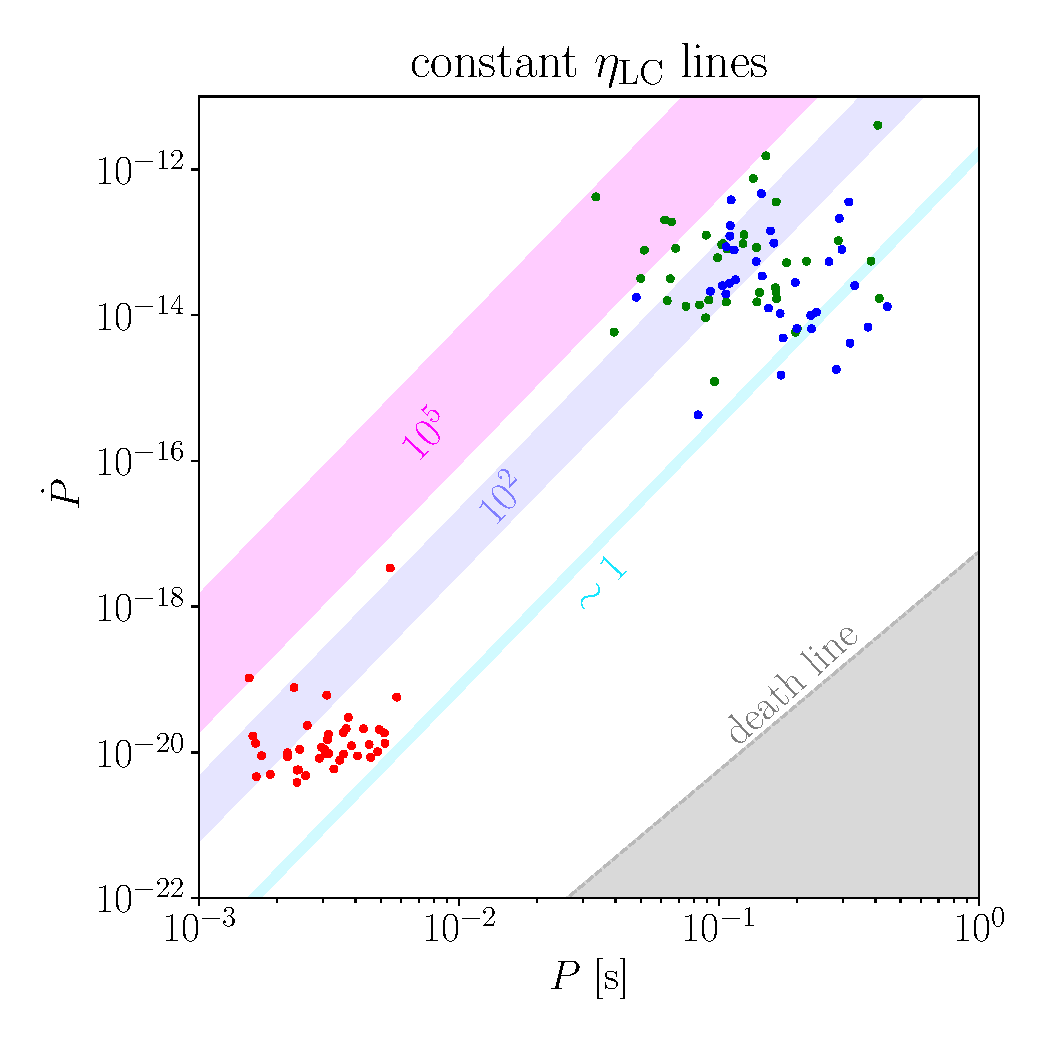
\includegraphics[width=\textwidth]{figures/ch4-pairproduction/fig13.pdf}
    }{
        \caption{Efficiency of the outer magnetosphere pair production in terms of the secondary plasma multiplicity, $\eta_{\rm LC}$, plotted against $P$ and $\dot{P}$ for all of the known $\gamma$-ray pulsars. Uncertainties of constant $\eta_{\rm LC}$ regions are due to varying the effective photon index (within $\Gamma\sim 1.5\text{-}2.5$). According to this figure, most of the $\gamma$-ray pulsars produce a substantial amount of secondary pairs in the outer magnetosphere.}
        \label{fig:pairprod-eta_th}
    }
\end{figure}

In Fig.~\ref{fig:pairprod-eta_th} we show our estimations for the secondary plasma multiplicity in the current sheet, $\eta_{\rm LC}$, computed using equation (\ref{eq:pairprod-eta_th}). Constant $\eta_{\rm LC}$ regions are plotted on a $P$-$\dot{P}$ diagram for known $\gamma$-ray pulsars, uncertainty of these regions are due to are due to the variation of the assumed photon index (within $\Gamma\sim 1.5\text{-}2.5$). As one can see, the majority of the observed $\gamma$-ray pulsars should be very efficient in producing secondary pairs, $\eta_{\rm LC}\gg 1$. Note, however, that here we assume the efficiency of polar pair production to be roughly $\kappa\sim 10^4$ for all pulsars, which might not be true (especially for the millisecond pulsars). Pulsars below $\eta_{\rm LC}\sim 1$ line ($X$-ray pulsars) will not have enough high energy radiation to substantially pair load the current sheet, and will thus have a much stronger dependency of the photon cutoff on the light cylinder magnetic field.

Our model also suggests that pair production in the outer magnetosphere may efficiently increase the density of the plasma escaping to the pulsar wind nebula. Observed injection rate of $X$- and $\gamma$-ray emitting particles to the PWN suggests multiplicities $\sim 10^4$ with respect to the average Goldreich-Julian density. This number is consistent with the upper limit provided by pair creation models from primary cascade near the polar cap \citep{2018arXiv180308924T}. However, observations of radio-emission from low energy plasma population implies a much higher limit on the ultimate multiplicity at the level of $10^5\text{-}10^6$ for  several different nebulae \citep{2010ApJ...720..266S, 2011MNRAS.410..381B, 2012SSRv..173..341A}. In this work we argue that on top of the primary cascade near the polar cap, two-photon pair production in the outer magnetosphere can further enhance the density of the outflowing plasma. This can account to the anomalously rich low-energy plasma population in the PWN observed in radio.

It is important to emphasize that in the present work we studied the optically thin regime to both Thomson scattering and pair production, with only synchrotron radiation enabled, and with pair production driven by the interactions of these synchrotron photons. While this regime is applicable to pulsars, the process of two-photon pair production in reconnecting regions is ubiquitous and might be important in a wide range of astrophysical environments, in regimes where other QED mechanisms may also be important. We list some examples below.\par

\begin{itemize}[leftmargin=*,wide = 0pt]
    \item {\it Black hole accretion disk coronae} are thought to sustain reconnecting current layers with enough $\sim$MeV photons to trigger the production of secondary pairs. This effectively increases the Thomson optical depth of the layer to unity \citep{1983MNRAS.205..593G, 1987MNRAS.227..403S, 1993ApJ...413..507H}. In this optically thick environment both the synchrotron and inverse-Compton (IC) cooling as well as the $e^-e^+$ annihilation are important to consider \citep{2017ApJ...850..141B}.
    \item {\it Blazar jet flares} with durations of several hours to days have been interpreted as powered by large and slow plasmoids in the reconnection layer, where two-photon pair production of IC photons may play a crucial role \citep{2012MNRAS.424L..26G, 2016MNRAS.462.3325P}.
    \item {\it Gamma-ray flares in SGRs} are also thought to be powered by relativistic reconnection with a near-critical magnetic field and with ongoing pair production driven primarily by $\gamma+B$ process (see, e.g., \citealt{2001ApJ...561..980T, 2006MNRAS.367.1594L}, studied in particle-in-cell by \citealt{2018arXiv180709750S})
\end{itemize}

The approach introduced in this work suggests a novel framework that could help to incorporate additional pair production effects in particle-in-cell simulations in a self-consistent way. We plan to continue improving our algorithms and investigating these unexplored regimes in future work.

% \appendix

%\chapter{Conclusion}
\label{conclusion}

Relativistic magnetic reconnection is a fast and efficient process of magnetic field dissipation, during which the energy stored in magnetic fields is extracted and deposited into plasma particles. Owing to its extremely violent character and the ability to accelerate particles to form non-thermal distributions, this process is thought to power many of the persistent and transient emission characteristics in compact astrophysical objects: from the magnetospheres of neutron stars and black holes to accretion disk coronae and jets. In many of these objects reconnection dynamics is also largely affected by the matter-light interaction, which may strongly alter their observational appearance. 

Up until now reconnection has been modeled using kinetic plasma simulations which mostly ignored these radiative effects. In \S\ref{ch:numerics} of this thesis I presented novel computational methods for including radiative and quantum electrodynamic (QED) effects in particle-in-cell plasma simulations. These techniques allow to self-consistently model plasma processes in extreme astrophysical conditions, where radiative reaction force is dynamically important, and the emitted light is strongly coupled to plasma via Compton scattering, two-photon pair production and $e^\pm$ pair-annihilation. I also proposed several simplified numerical experiments to test the performance of these algorithms and compare the outcome with the analytic predictions. 

Reconnection can accelerate particles to ultra-relativistic energies generating a non-thermal power-law distribution. The maximum energy of this distribution, as well as the power-law index are thought to be uniquely controlled by the so-called magnetization parameter in the upstream unreconnected plasma. In \S\ref{ch:plasmoids}, I explored a new powerful acceleration channel during magnetic reconnection that allows to overcome the previously known limit on the maximum energy, and form a broken power-law. This acceleration mechanism operates in continuously compressing magnetic islands, called plasmoids, that form in the non-linear stage of the reconnection and carry away the reconnected flux and energized particles. Theoretical model of this process allowed me to extrapolate its implications to real astrophysical systems. This mechanism may explain the observed broken power-law distributions and anomalously high energies in some of the blazar jets.

Macroscopic current layers are thought to emerge in the magnetospheres of neutron stars as a result of the large-scale magnetic topology. Magnetic reconnection in these layers may dissipate a significant amount of Poynting flux carrying away the rotational power of the neutron star. In \S\ref{ch:pulsar}, I recreated the magnetospheres of neutron stars in PIC simulations and from first principles reproduced the reconnection plasma dynamics in the current layer. I demonstrated that microscopic plasma physics in the thin reconnecting layer controls the overall energy dissipation rate in the entire magnetosphere. The fraction of energy dissipated is uniquely set by the rate of magnetic reconnection, and appears to be insensitive to synchrotron radiation efficiency and bulk motion of the magnetospheric wind. I have also studied the acceleration of particles during reconnection and resulting synchrotron spectra for pulsars in different radiative regimes. I provided a possible explanation for why pulsars with higher spin-down power and stronger synchrotron cooling typically exhibit $\gamma$-ray spectra that peak at lower energies. 

In the most energetic $\gamma$-ray pulsars, such as the Crab, synchrotron emission in the current layer is so abundant and energetic that the emitted photons can interact with each other producing secondary $e^\pm$ pairs. In \S\ref{ch:pairproduction}, I studied this process by self-consistently coupling photon emission and two-photon pair production process to plasma simulations of the magnetically reconnecting current layer. In certain regimes pair production is so abundant that the current layer is dominated by the pairs produced \emph{in-situ}. This process feeds the radiated energy back into the current sheet in the form of secondary pairs, inhibiting the acceleration efficiency of reconnection. As a result, a negative feedback loop emerges, which controls the overall particle acceleration efficiency. This effect explains the universality of $\gamma$-ray cutoff energies in young pulsars, which is around few to $10$ GeV and is surprisingly insensitive to the strength of the magnetic field in the reconnecting current layer.

\subsection*{\small \it Future prospects}

Large-scale reconnecting current layers can be intermittently produced in \emph{the magnetically arrested accretion disks} of supermassive black holes (such as the one in M87; see, e.g., \citealt{2020ApJ...900..100R,ripperdainprep}). Parameter regimes in these layers are close to those in $\gamma$-ray pulsars: the synchrotron cooling efficiency is marginal and the two-photon pair production process is abundant. These transient reconnection events most likely power the observed TeV flares \citep[see, e.g.,][]{2006Sci...314.1424A} by upscattering soft background photons on pair plasma energized during reconnection. Modeling radiative reconnection in this regime to reproduce the emerging TeV emission, as well as the lower energy counterpart, is the next logical step in this topic. 

In the hard states of X-ray binaries millisecond-duration $\gamma$-ray flares \citep[see, e.g.,][]{2003MNRAS.343L..84G} are thought to be powered by transient reconnection events from disrupting magnetic flux ropes in \emph{the accretion disk coronae} \citep{1979ApJ...229..318G,2008ApJ...682..608U,2017ApJ...850..141B}. In these environments, synchrotron and inverse Compton cooling are very efficient, while the optical depth of the emission (which is close to unity) is self-consistently controlled by the balance between two-photon pair production and electron-positron annihilation. Dynamics of the reconnection has never been studied in such an exotic regime.

In \emph{magnetars}, non-linear Alfv\'enic fluctuations generated at the surface of the star may disrupt the magnetosphere, producing large-scale reconnecting current sheets \citep{2020arXiv201107310B,2020ApJ...900L..21Y}. Emission from these current sheets may be responsible for the observed $\gamma$-ray flares and short-duration X-ray bursts \citep{2017ARA&A..55..261K}. Simulations show that similar dynamics may occur in the coupled magnetospheres of \emph{the coalescing binary neutron stars} shortly before they merge \citep{2020ApJ...893L...6M}. Since the parameter regimes are very close in these systems, this transient would generate a strong high-energy precursor to the neutron star merger event. In the regimes applicable both to magnetar flares and binary neutron stars, pair-production and annihilation are self-balanced, while the Compton scattering is so violent that it can effectively couple plasma to radiation, providing an effective ``photon viscosity'' and possibly strongly inhibiting the reconnection process. 

In this thesis I described a novel set of tools and techniques for modeling plasma kinetics (such as reconnection, turbulence, collisionless shocks, etc) mediated by radiative and QED processes. This extreme regime has largely been beyond the reach of first-principle plasma simulations, and many of the observational implications have been overlooked. My thesis is intended to serve as one of the first steps towards enabling us to reproduce and understanding the microscopic plasma behavior in these violent environments. Above I presented just a few of the examples of systems where radiative and QED processes may play a vital role both in terms of the fundamental plasma physics, and also in terms of interpreting the observations from compact sources.

%\begin{appendices}
    %\chapter{}
\section{Cross sections for the QED processes}
\label{appendix:num-crosssections}

In this appendix we present the expressions for the differential and total cross sections of three different QED processes included in \texttt{Tristan-MP v2} and described in section~\ref{sec:num-QED}. All the expressions are taken from the book by \cite{1985quel.book.....A}. In this section $\sigma_T$ is the Thomson cross section, $d\Omega$ is the differential solid angle, and $\theta$ is the scattering angle between the initial and final momenta; all the energies are normalized to $m_e c^2$. Also notice, that the total cross section is a relativistic invariant.

For \emph{Compton scattering} of a photon on an electron (or positron) it is convenient to express the cross sections in the $e^\pm$ rest-frame:
\begin{equation}
    \begin{aligned}
        \frac{d \sigma_C}{d\Omega} &= \frac{3}{16\pi} \sigma_T 
            \frac{1 + \cos^2{\theta}}{\left(1 + \varepsilon_1(1-\cos{\theta})\right)^2}
            \left(1 + \frac{\varepsilon_1^2(1-\cos{\theta})^2}{(1+\cos^2{\theta})\left(1 + \varepsilon_1 (1-\cos{\theta})\right)}\right),\\
        \sigma_C &= \frac{3}{4}\sigma_T\left[
            \frac{1+\varepsilon_1}{\varepsilon_1^3}
                \left( \frac{2\varepsilon_1(1+\varepsilon_1)}{1+2\varepsilon_1} - \ln{(1 + 2\varepsilon_1)}\right)
            + \frac{\ln{(1+2\varepsilon_1)}}{2\varepsilon_1} - \frac{1 + 3\varepsilon_1}{(1 + 2\varepsilon_1)^2},
        \right]
    \end{aligned}
\end{equation}

\noindent where $\varepsilon_1$ is the energy of the photon before the scattering (in the  $e^\pm$ rest-frame).

For \emph{two-photon pair production} process the cross sections are given in the center-of-momentum frame of the two interacting photons:

\begin{equation}
    \begin{aligned}
        \frac{d \sigma_{\gamma\gamma}}{d\Omega} &= \frac{3}{32\pi} \sigma_T 
            \frac{\sqrt{\varepsilon_0^2-1}}{\varepsilon_0^3}
            \left[
                \frac{2 \varepsilon_0^2 -1 + (\varepsilon_0^2 - 1)\sin^2{\theta}}{\cos^2{\theta} + \varepsilon_0^2\sin^2{\theta}}
                - \frac{2(\varepsilon_0^2 - 1)^2\sin^4{\theta}}{\left(\cos^2{\theta}+\varepsilon_0^2 \sin^2{\theta}\right)^2}
            \right] \\
        \sigma_{\gamma\gamma} &= \frac{3}{8}\sigma_T \frac{1}{\varepsilon_0^2}\left[
            \left(2 + \frac{2}{\varepsilon_0^2} - \frac{1}{\varepsilon_0^4}\right)\ln{\left(\varepsilon_0 + \sqrt{\varepsilon_0^2 - 1}\right)} - 
            \sqrt{1 - \frac{1}{\varepsilon_0^2}}\left(1 + \frac{1}{\varepsilon_0^2}\right)
        \right],
    \end{aligned}
\end{equation}

\noindent where $\varepsilon_0$ is the energy of either of the photons in the center-of-momentum frame. For two photons with energies $\varepsilon_1$ and $\varepsilon_2$ in an arbitrary frame with an incident angle $\phi$ w.r.t. each other we find: 
\begin{equation}
    \varepsilon_0 = \frac{1}{2}\frac{\varepsilon_1 \varepsilon_2}{(m_e c^2)^2}\left(1-\cos{\phi}\right).
\end{equation}

\noindent Notice, that this interaction is prohibited if $\varepsilon_0 < 1$, i.e., if the total energy of the interacting photons in the center-of-momentum frame is less than $2m_e c^2$.

For \emph{pair-annihilation} the cross sections are also given in the center-of-momentum frame of the interacting electron and positron:

\begin{equation}
    \begin{aligned}
        \frac{d \sigma_{\rm ann}}{d\Omega} &= \frac{3}{32\pi} \sigma_T \frac{1}{v_0 \varepsilon_0^2}
        \frac{1+v_0^2\sin^2{2\theta} - v_0^4(1 - \sin^4{\theta})}{\left(1 - v_0^2\cos^2{\theta}\right)^2 },\\
        \sigma_{\rm ann} &= \frac{3}{32}\sigma_T \frac{1}{v_0\varepsilon_0^2}
        \left(
            \frac{3-v_0^4}{v_0} \ln{\left|\frac{1+v_0}{1-v_0}\right| + 2(v_0^2 - 2)}
        \right)
        ,
    \end{aligned}
\end{equation}

\noindent with $\varepsilon_0$ and $v_0$ being, correspondingly, the energy and the magnitude of the three-velocity of either of the interacting particles in the center-of-momentum frame.
    %\chapter{}
\section{Structure of the plasmoid shell}
\label{appendix:rec-plasmashell}

This appendix focuses on the internal structure of primary isolated plasmoids. We estimate the power-law indices, defined by Equation~\eqref{eq:rec-radialstruct}, of the radial profiles of the magnetic field and plasma density inside the plasmoid shell, $\rins < r < r_0(t)$. We also derive how the distance of particles from the plasmoid center decreases with time, as particles slowly descend toward it.

First, let us assume that at any given radius from the center of the plasmoid there is a balance between the magnetic forces and plasma pressure
\begin{equation}
    \label{eq:rec-forcebalance}
    \frac{1}{c}\bm{j}\times\bm{B} = \nabla P,
\end{equation}
where the current density $\bm{j}$ can be expressed as $4\pi\bm{j}/c=\nabla\times\bm{B}$. Motivated by the simulation results, we assume that, within the plasmoid shell, $\bm{B}$ is purely toroidal and the only variation occurs in the radial direction, i.e., $\bm{B}=B(r)\bm{\hat{\phi}}$. Then, Equation~\eqref{eq:rec-forcebalance} can be rewritten as
\begin{equation}
    \label{eq:rec-b1}
    -\frac{B^2}{r} = \frac{d}{dr}\left(4\pi P + \frac{B^2}{2}\right) \cdot
\end{equation}

We also assume a polytropic EOS for the plasma inside the plasmoid shell, with isotropic pressure
\begin{equation}
    \label{eq:rec-state}
    P = K\rho^\Gamma,
\end{equation}
where $K$ is some dimensional constant and $\Gamma$ is the adiabatic index. Substitution of Equations~\eqref{eq:rec-radialstruct} and  \eqref{eq:rec-state} into Equation~\eqref{eq:rec-b1} yields
\begin{equation}
\label{eq:rec-b2}
    \frac{(1-\zeta)\sigma_0}{\xi(\Gamma-1)} = \left(\frac{r}{r_0(t)}\right)^{2\zeta-\xi\Gamma},
\end{equation}
where $\sigma_0$ is the plasma magnetization at $r=r_0$. This can be expressed as
\begin{equation}
    \label{eq:rec-sigma0}
    \sigma_0 \approx \frac{B_0^2(\Gamma-1)}{4\pi \Gamma K\rho_0^\Gamma},
\end{equation}
where we used the definition for the plasma magnetization $\sigma_0 = B_0^2/4\pi h_0$, and expression of the enthalpy density $h_0$ (at $r=r_0$) for a relativistically hot plasma ($kT_0 \gg m_e c^2$)
% We set our boundary conditions at $r=r_0$, by defining the magnetization in the plasmoid shell, $\sigma_0 = B_0^2/4\pi h_0$, where $h_0$ is the enthalpy at $r=r_0$. For the relativistically hot plasma in the plasmoid shell ($T_0\gg m_e c^2$) we may write that
\begin{equation}
    h_0 = \rho_0 c^2\left(1 + \frac{\Gamma}{\Gamma-1} \frac{kT_0}{m_e c^2}\right) \approx \frac{\Gamma}{\Gamma-1} P_0,
\end{equation} 

For Equation~\eqref{eq:rec-b2} to be satisfied at all times and for all $\rins <r\le r_0$, the following relations must hold:
% and $t$ if and only if
\begin{equation}
    2\zeta=\xi\Gamma,~\text{and}~(1-\zeta)\sigma_0=\xi(\Gamma-1).
\end{equation}
Solving the above equations for the unknown power-law indices $\zeta$ and $\xi$, we find
\begin{equation}\label{eq:rec-powerlaws_app}
    \zeta=\frac{\Gamma\sigma_0/2}{\Gamma + \Gamma\sigma_0/2 - 1},~\text{and}~\xi = \frac{\sigma_0}{\Gamma + \Gamma\sigma_0/2 - 1} \cdot
\end{equation}

Particles inside the plasmoid shell are frozen into the slowly contracting magnetic field loops, which bring the particles closer to the plasmoid center. As a result, the mass enclosed within a fixed magnetic loop in the plasmoid shell is approximately constant in time. This condition can be expressed as
\begin{equation}
    \int_{\rins}^{\Rlg}r \rho(r, t)dr \approx \mathrm{const},
\end{equation}
where $\Rlg$ is the decaying radius of a fixed magnetic loop or plasma ring (see Figure~\ref{fig:rec-layerevol}). 
This condition, together with Equations~\eqref{eq:rec-radialstruct} and \eqref{eq:rec-inflationrate}, yields
\begin{equation}
    \label{eq:rec-lagrangian_radius}
    \Rlg\propto r_0(t)^{-\xi/(2-\xi)} \propto t^{-\kappa\xi/(2-\xi)}
\end{equation}
where we assumed $\rins \ll \Rlg$.

As an example, Figure~\ref{fig:rec-plasm_eos} shows results from our simulations (for a description, see Section~\ref{sec:reconnection-setup}) for $\sups=10$ (top row) and $100$ (bottom row). Panels (a) and (d) show the region of the plasmoid where the force balance is satisfied, panels (b) and (e) show magnetization as a function of radius from the plasmoid center (blue shaded region corresponds to the same region in (a) and (d)), and panels (c) and (f) show the EOS for the same region (top and bottom panels correspond to different upstream magnetizations, $\sigma_{\rm up}=10$ and $\sigma_{\rm up} = 100$). As we see from panels (b) and (e), the effective magnetization drops from the upstream value to a roughly constant value $\sigma_0\approx 1$ in the plasmoid shell. From panels (c) and (f) we can see that the EOS indeed looks like a polytrope with a characteristic adiabatic index of $\Gamma=4/3$. 

Thus, for $\Gamma=4/3$ and $\sigma_0\approx 1$ from Equation \eqref{eq:rec-powerlaws_app} we find that $\zeta\approx 2/3$ and $\xi \approx 1$. From Equation \eqref{eq:rec-lagrangian_radius} we also find that $\Rlg\propto t^{-\kappa}$ when $\xi\approx 1$.

\begin{figure}[htb]
    \centering
    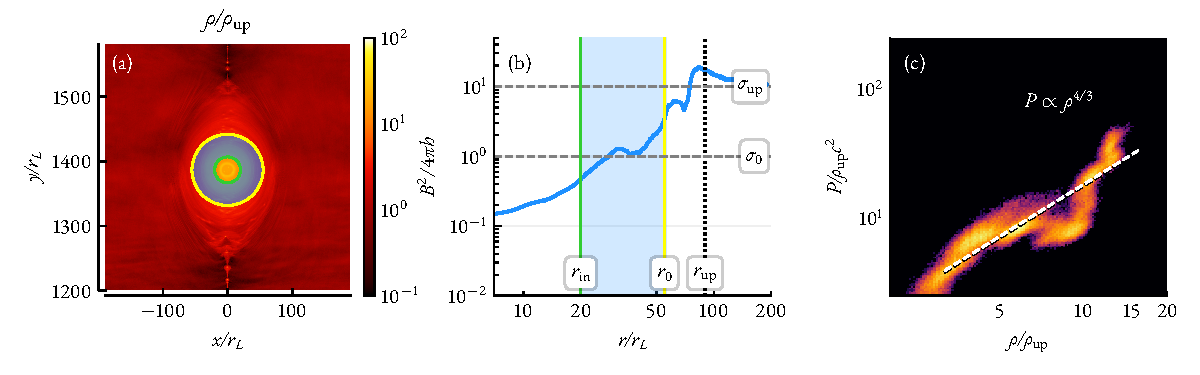
\includegraphics[width=\textwidth]{figures/ch2-reconnection/figa1_1.pdf}
    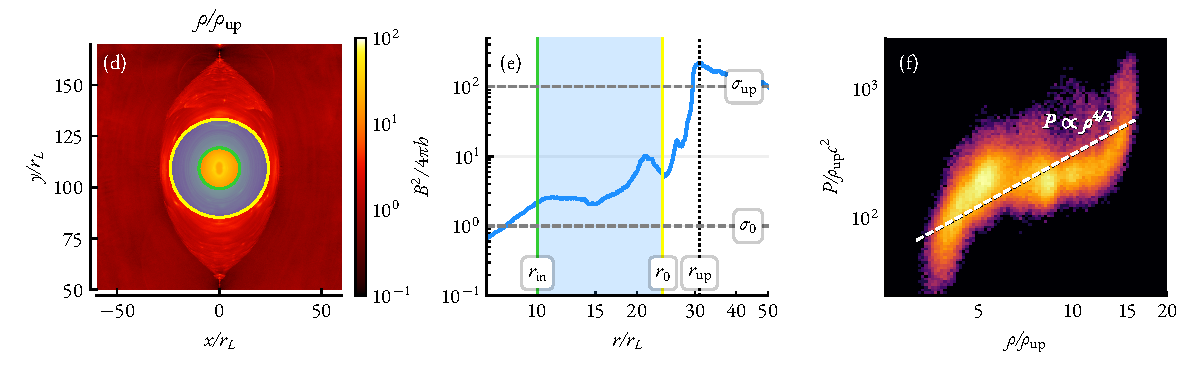
\includegraphics[width=\textwidth]{figures/ch2-reconnection/figa1_2.pdf}
    \caption{Top panels correspond to the $\sups=10$ simulation, while bottom panels are for the $\sups=100$ case. (a, d) Close-up view of an isolated primary plasmoid, with color indicating $\rho/\rho_{\rm up}$ (see color bar). The plasmoid shell, where the force balance condition \eqref{eq:rec-forcebalance} is satisfied, is shown as a blue shaded ring; the green and yellow circles indicated the core radius and the boundary of the shell. (b, e) Plasma magnetization as a function of radius from the plasmoid center (in units of $r_L$). The blue shaded region corresponds to the plasmoid shell, shown in blue in panels (a) and (d). The horizontal dashed lines correspond to the upstream magnetization, $\sups$, and the magnetization of the plasmoid shell, $\sigma_0$ (see Equation~\eqref{eq:rec-sigma0}). The three radii marked on the plot are defined in Section~\ref{sec:reconnection-plasmoids}. (c, f) Typical two-dimensional histogram of the plasma pressure and plasma density for the shaded region in panels (a) and (d). The polytropic EOS for a relativistic gas is also shown (dashed line).}
    \label{fig:rec-plasm_eos}
\end{figure}

\section{Finding the boundaries of plasmoids}
\label{appendix:rec-plasmbound}
In this section, we describe the algorithm we used for identifying the plasmoid boundaries. This relies on the mixing criterion~\citep{2014PhPl...21e2307D, 2017ApJ...850...29R} and on the vector potential.

We distinguish particles originating from one side of the current sheet, $+x$, from the ones from the other side, $-x$. Henceforth, we refer to their densities as $\rho^+$ and $\rho^-$. We then compute the so-called {\it mixing factor}, $\lambda_f$, in each cell of our simulation domain

\begin{equation}
    \lambda_f = 1 - \left(1 - 2\frac{\rho^+}{\rho^+ + \rho^-}\right)^2.
    \label{eq:rec-mixingf}
\end{equation}

The mixing factor is defined in a way that $\lambda_f = 1$ inside the plasmoids and the current sheet, where particles from two separated regions are perfectly ``mixed,'' and $\lambda_f = 0$ everywhere else. At the plasmoid edges the mixing factor takes intermediate values, $0 < \lambda_f < 1$ (see Figure~\ref{fig:rec-plasmbound}(b)). We compute the isocontours of the vector potential $A_z$ (the simulation is done in the $x$-$y$ plane). To identify the boundary of a particular plasmoid, we select regions characterized by intermediate values of the mixing factor (i.e.,  $0.1 < \lambda_f < 0.9$) and find the average value of the vector potential values in these regions, $A_z^0$. We then define the isocontour of $A_z=A_z^0$ as the boundary for that particular plasmoid (see Figure~\ref{fig:rec-plasmbound}(a), thick white line).

\begin{figure}[!ht]
    \centering
    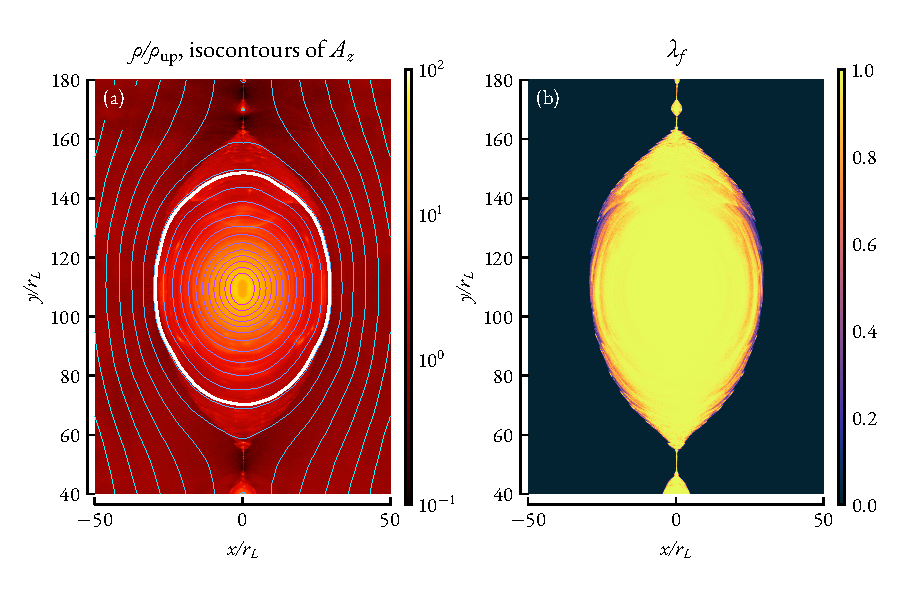
\includegraphics[width=\textwidth]{figures/ch2-reconnection/figb1.pdf}
    \caption{Zoom in of a small region of the reconnection layer (from the $\sups=100$ simulation) containing an isolated large plasmoid. Panel (a) Plasma density in logarithmic scale (see color bar on the side)  with overlaid contours of the vector potential (solid cyan lines). The thick white line corresponds to $A_z=A_z^0$ and marks the plasmoid boundary. (b) Mixing factor, $\lambda_f$, defined by Equation~\ref{eq:rec-mixingf}. The transition from $\lambda_f=1$ (fully mixed) to 0 (not mixed) happens over only a few skin depths.}    
    \label{fig:rec-plasmbound}
\end{figure}

Our results are robust to the choice of the exact mixing factor values, as $\lambda_f$ has a very steep spatial profile at the plasmoid edges; it changes quickly from $0$ to $1$ going from the upstream to the plasmoid within a few skin depths, meaning that the mixing of particles happens very abruptly. Even if one argues that our method does not yield the exact plasmoid boundary, this does not affect our results, because our analysis focuses on long-term processes taking place well within the plasmoid boundary.

    %\chapter{}
\section{Details on the pair-production algorithm}
\label{sec:pairprod-appendixA}

Since this is the first implementation of the self-consistent pair production in a particle-in-cell code, in this Appendix we present the details about the algorithm we used in our simulations.

\begin{figure}[htb]
    \centering
    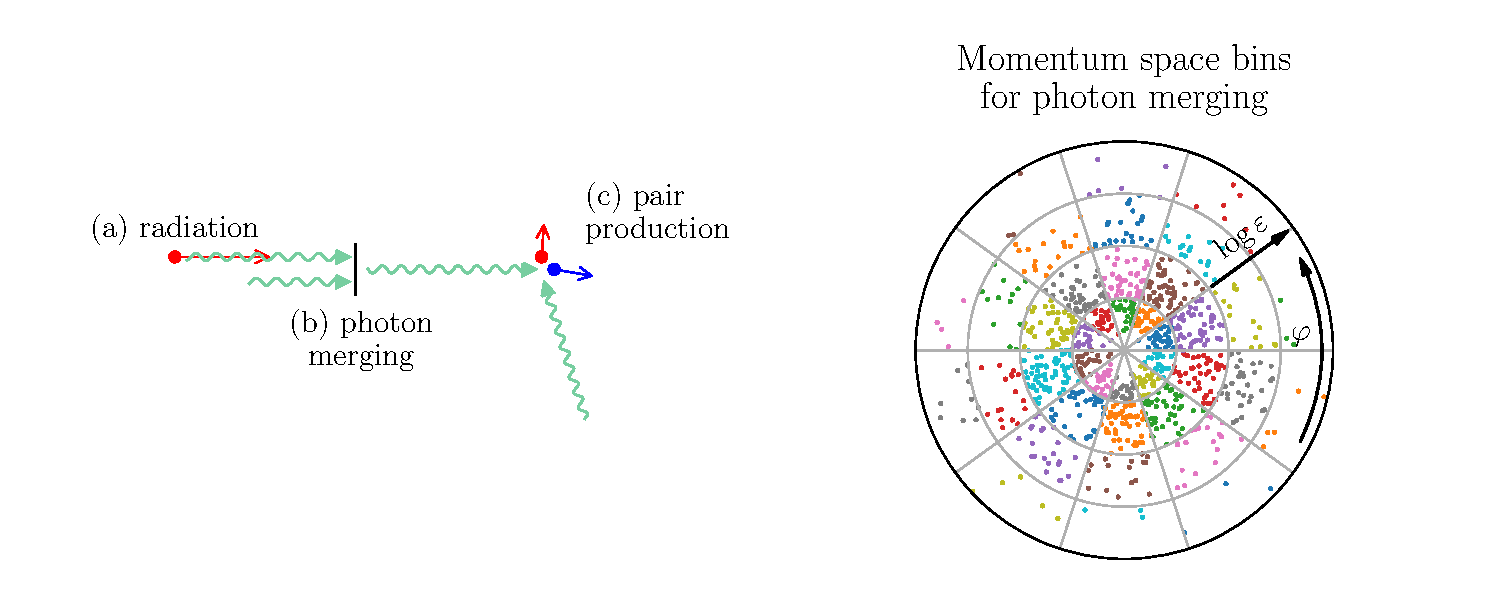
\includegraphics[width=.8\textwidth]{figures/ch4-pairproduction/fig_a1.pdf}
    \caption{{\it Left}: three main steps in our algorithm -- plasma particle radiation a photon, photons merging (downsampling) in a given cell, photons interacting and producing secondary pairs. {\it Right}: two-dimensional version of the momentum binning we use for the photon downsampling. Binning is logarithmic in energy (momentum magnitude) and uniform in direction. Photons are colored according to their location in those bins, all the photons of the same color will be merged into two photons with higher weights conserving energy and momenta.}
    \label{fig:pairprod-alg_scheme}
\end{figure}

We track two particle species: charged and massive plasma particles and massless photons. At each timestep a plasma particle can radiate a photon (step (a) in Figure~\ref{fig:pairprod-alg_scheme}, {\it left}) with a corresponding synchrotron energy given by formula (\ref{eq:pairprod-synch_form}), and the overall cooling rate is set by relation (\ref{eq:pairprod-synch_rate}). The photons are then resorted in memory according to their spatial location.

Since we intend to study the optically thin regime to pair production, $\tau_{\gamma\gamma}\ll1$, and at the same time we have a sufficiently high multiplicity of secondary pairs, in our simulations the typical number of photons greatly exceeds the number of particles. This can very quickly exhaust the memory capabilities. To avoid this we use a downsampling (merging) algorithm for the photons similar to one described by \cite{2015CoPhC.191...65V}.

In each simulation cell we define three-dimensional photon momentum bins and sort photons according to their momenta as seen in Figure~\ref{fig:pairprod-alg_scheme}, {\it right}. The bins are logarithmic in photon energies and uniform in 3D directions. We also randomly ``rotate'' the bins to minimize any downsampling artifacts. All the photons in the same momentum bin are then merged into two photons with higher effective weights (step (b) in Figure~\ref{fig:pairprod-alg_scheme}, {\it left}), conserving total energy and momentum. Note also, that since the downsampling is done for the lowest energy photons (which are the majority) and for those who have small relative momenta angles, downsampling does not strongly affect the pair production efficiency, since those photons have a negligible probability to pair produce.

Two-photon pair production (step (c) in Figure~\ref{fig:pairprod-alg_scheme}, {\it left}) is another expensive step that we implement in our simulation. At each cell we loop through all the non-repetitive pairs of photons and compute their binary probabilities $p_{ij}$ to pair produce given their energies, momenta and the cross section formula.

Since the weights of those photons can be greater than one, these probabilities as well can exceed unity, i.e., if $p_{ij}=4.2$ on average from these photons $i$ and $j$ we will create $4.2$ $e^-e^+$ pairs: $4$ pairs with a probability $1$ and one more pair with a probability $0.2$ (reducing the photon weights each time). This approach is designed to mimic as if these interactions were between independent photons not merged into a two ``heavy'' ones.

The probability magnitudes are normalized to a fiducial parameter, $p_0$, which is chosen to ensure the low optical depth to pair production. Overall the optical depth for a photon can be written as
\begin{equation}
    \tau_{\gamma\gamma} = L\langle n_{\rm ph}\rangle f_0 p_0,
\end{equation}
where $L$ is the effective size of the system, $\langle n_{\rm ph}\rangle$ is the average number of (potentially pair producing) photons per cell along the path, $p_0$ is our fiducial parameter, and the prefactor $f_0$ accounts for the cross section for different energies and momenta orientation (see Figure~\ref{fig:pairprod-sigma_pp}) and is typically $0.1\text{-}0.01$. In our simulations the size of the system is typically a few times $10^3$ cells, and the effective number of pair producing photons along the path can vary $10^2\text{-}10^3$ (less than the total number of photons per cell). This gives us a rough estimate that
\begin{equation}
    \tau_{\gamma\gamma} \sim \frac{p_0}{10^{-3}}.
\end{equation}

The difference between optically thick and thin regimes is demonstrated in Figure~\ref{fig:pairprod-opt_thick}. The evolution of a single photon generation spectra are different in these two cases ($p_0=10^{-3}$ and $p_0=10^{-5}$). In optically thick regime (Figure~\ref{fig:pairprod-opt_thick}, {\it right}) most of the high energy photons interact with lower energy ones and pair produce in less than a single light-crossing time, resulting in a lower cutoff energy, whereas in optically thin regime (Figure~\ref{fig:pairprod-opt_thick}, {\it left}) the spectrum nearly uniformly drops down over all energies due to pair production in a few light-crossing times.

\begin{figure}[htb]
    \centering
    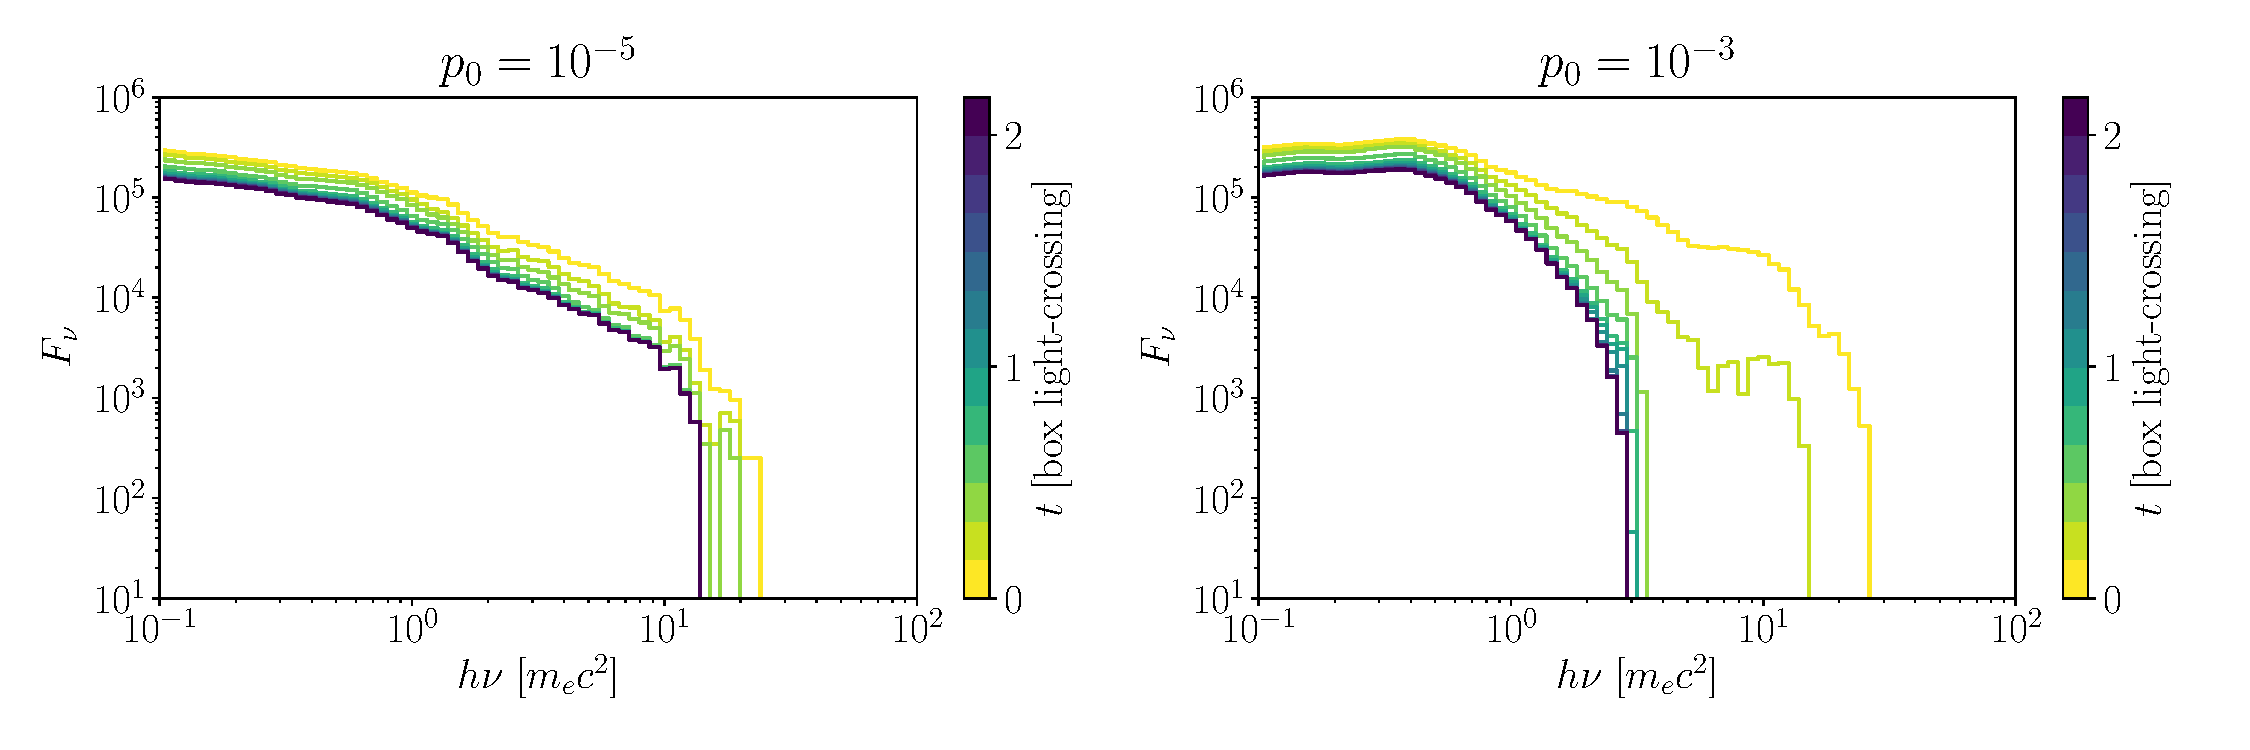
\includegraphics[width=.8\textwidth]{figures/ch4-pairproduction/fig_a2.pdf}
    \caption{Time evolution of the spectrum of photons born at the same timestep. The time is measured in box light-crossing times, {\it left} plot corresponds to an optically thin regime with $p_0=10^{-5}$, and {\it right} -- optically thick with $p_0=10^{-3}$. Spectra are corrected to photons leaving the box, i.e., the reduction is only due to pair production. In optically thick regime most of the high energy photons interact in less than a light-crossing time.}
    \label{fig:pairprod-opt_thick}
\end{figure}

\begin{table}
\begin{centering}
 \begin{tabular}{ l || c | c }
 \hline
  & Computational cost & Memory usage \\ [0.5ex]
 \hline\hline
 photon sorting & $\mathcal{O}(N_{\rm ph})$ & $\mathcal{O}(N_{\rm ph})$ \\
 photon merging & $\mathcal{O}(N_{\rm ph})$ & $\mathcal{O}(n_{\rm ph})$ \\
 pair production & $\mathcal{O}(n_{\rm ph} N_{\rm ph})$ & $\mathcal{O}(N_{\rm ph})$ \\ [1ex]
 \hline
\end{tabular}
\caption{Time and memory costs for the most expensive parts of our algorithm as a function of the total number of photson in the box, $N_{\rm ph}$, and the average number of photons in each cell, $n_{\rm ph}$. }
\label{table:comp}
\end{centering}
\end{table}

Finally, in Tab.~\ref{table:comp} we present the time and memory consumption of our algorithm as a function of the total number of photons, $N_{\rm ph}$, and the average number of photons per simulation cell, $n_{\rm ph}$. Pair production is the most expensive procedure, since it is $\sim\mathcal{O}(n_{\rm ph}^2 N_{\rm cells}) \sim \mathcal{O}(n_{\rm ph} N_{\rm ph})$.

Merging is efficient as far as the average number of photons per cell is $n_{\rm ph}\gg N_{\rm bins}$, where the number of momentum bins we typically use is $N_{\rm bins}=8^3=512$. In our typical run we have $10^4\text{-}10^5$ photons per cell, and, thus, this downsampling significantly decreases the cost by reducing the number of tracked photons typically by a factor of $10\text{-}100$.

In most of our runs this is still expensive, and we do this procedure once every several steps, instead of doing it every step. One, however, should keep in mind, that this interval cannot be longer than the typical mean free path of the photons to pair production (which in our case is a fraction of the box size), and also the interval should be short enough for the merging to prevent the memory exhaustion.


\section{Radiation and pair production statistics}
\label{sec:pairprod-appendixB}

We also present several diagnostic plots to justify our assumptions made earlier. Figure~\ref{fig:pairprod-phot_born} ({\it left}) shows the two-dimensional histogram of the number of produced synchrotron photons plotted against the plasma particle energy and effective magnetic field that a particle experienced when radiating. Contour lines show the corresponding synchrotron energies.

One can see that most of the photons are produced in a narrow range of magnetic field values from $0.1B_0$ to $B_0$, and the range gets even smaller for the higher energy particles, which are interesting in terms of pair production. Also it is clear that most of the photons are very low energy, which, however, do not strongly contribute to pair production. Thus, it is important to correctly set the minimum tracking energy to make sure to capture enough pair production, but at the same time not to overwhelm the memory.

\begin{figure}[tb]
    \centering
    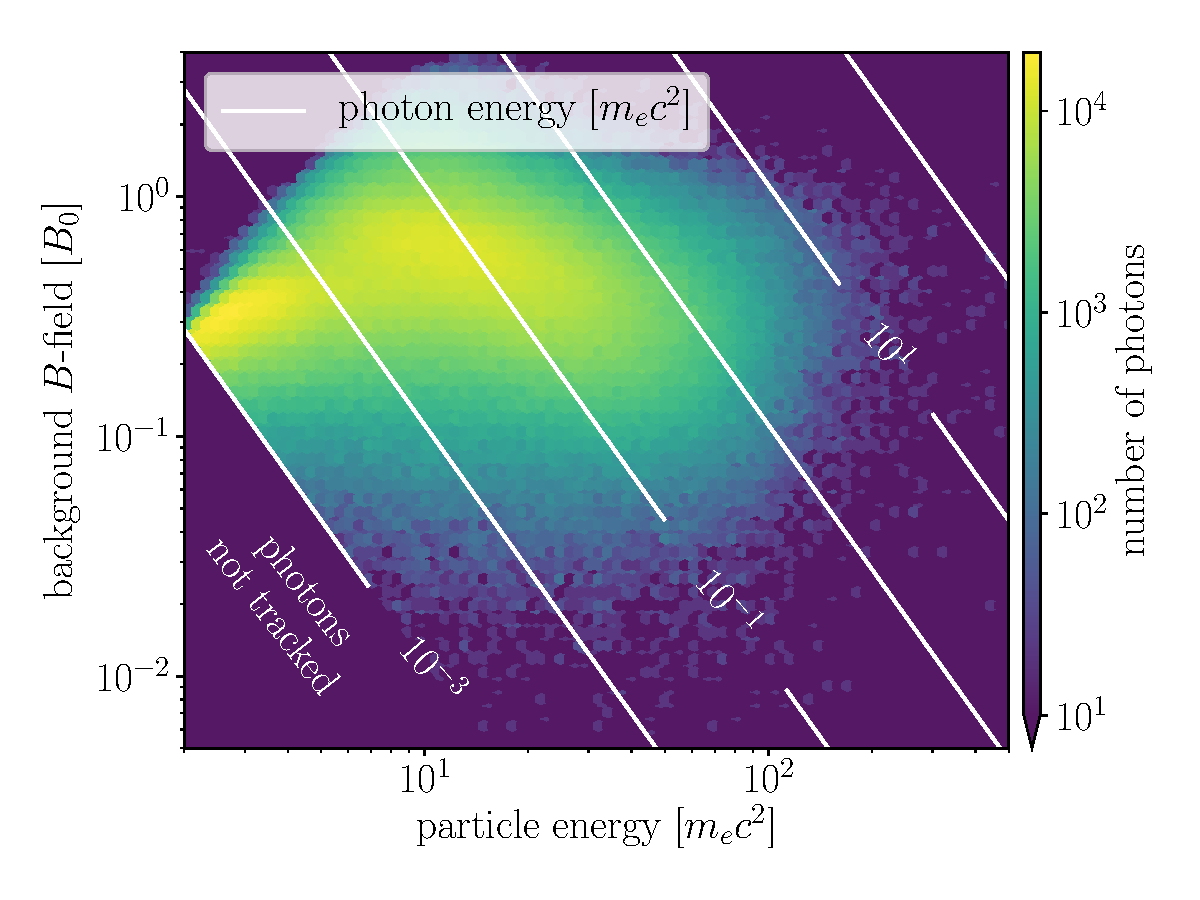
\includegraphics[width=0.5\textwidth]{figures/ch4-pairproduction/fig_b1.pdf}
    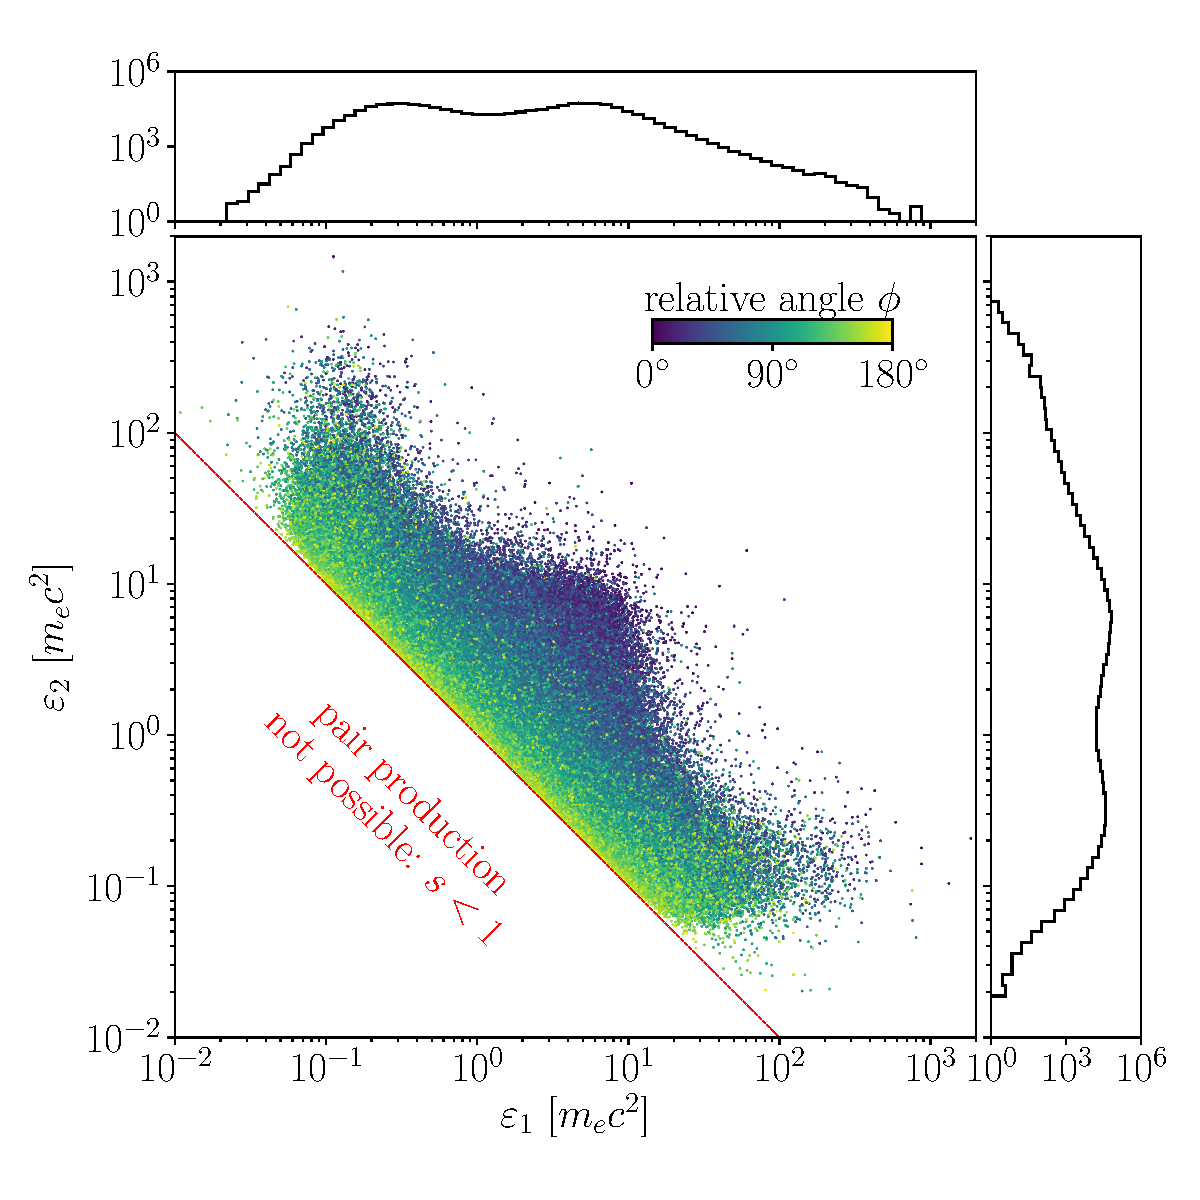
\includegraphics[width=0.4\textwidth]{figures/ch4-pairproduction/fig_b2.pdf}
    \caption{{\it Left:} 2D histogram of the radiated synchrotron photons vs the particle energy and the background magnetic field from one of our simulations ($\sigma_{\rm c}=5000$, $\gamma_c=50$, $\gamma_{\rm rad}=200$, $p_0=10^{-5}$). Each particle radiates at a corresponding synchrotron frequency (white contours), set by an effective background magnetic field (y-axis) and the Lorentz-factor of the particle (x-axis). Photons below $10^{-3}m_e c^2$ are not tracked, since they do not participate in pair production. {\it Right:} pair production statistics from the same simulation as on the left. Each point is a pair production event with $x$ and $y$ axes corresponding to the interacted photon energies and colors corresponding to their relative angles. One dimensional histograms are shown above and to the right, demonstrating that a wide range of photon energies are roughly equally important in terms of pair production.}
    \label{fig:pairprod-phot_born}
\end{figure}

Figure~\ref{fig:pairprod-phot_born} ({\it right}) shows the statistics of pair production from the same run, scatter plotted against the energies of two photons that produced the pairs. Each point is the pair production event, the color of each point represents the relative angle, $\phi$, between photon momenta. As one could have anticipated, the closer the energy product $\varepsilon_1\varepsilon_2$ to $2m_e c^2$, the closer the relative angle to $180^{\circ}$, and vice versa: two high energy photons can interact if their relative angle is small.

As one can also see from the one-dimensional histograms (Figure~\ref{fig:pairprod-phot_born}, {\it right}), the majority of pair production is for the photon energies $\varepsilon>10^{-2}m_e c^2$, and, thus, the photon tracking energy limit (which in this case is $10^{-3} m_e c^2$) is justified. Two extended scatter ``wings'' to the right and up are due to the fact that some very high energy photons do not have a low energy partner to interact (not tracked), and are left to interact with the higher energy ones. These tails, while being a numerical artifact, however, do not contribute much to pair production. We have carried convergence tests with lowering the energy limit with similar results: very low energy photons do not have a a significant contribution to pair production.

In Figure~\ref{fig:pairprod-energy_vs_time} the distribution of total energy in the box between different components is shown (normalized by the initial magnetic field energy, $U_B$). After the reconnection is triggered we let the initial plasma to escape through the boundaries perpendicular to the current sheet, which are being opened at around 1-2 light crossing times. After that new plasma (and thus magnetic flux) is injected at the boundaries, carrying additional energy, which is why we see that first spike in the plot. Most of the energy is carried by the magnetic field which in the process of regular reconnection is being transferred to primary generation of particles up to 2-3 box light-crossing times. At that point the synchrotron cooling and pair production are turned on and the reconnection relaxes to a new steady state.

At late times the energy is mostly contained in photons and secondary particles created in pair production events. The large ``waves" lasting a few box light-crossing times at late times are due to the large plasmoid, that constantly form, accumulate secondary plasma from the environment, and are then advected out from the box.

\begin{figure}[tb]
    \centering
    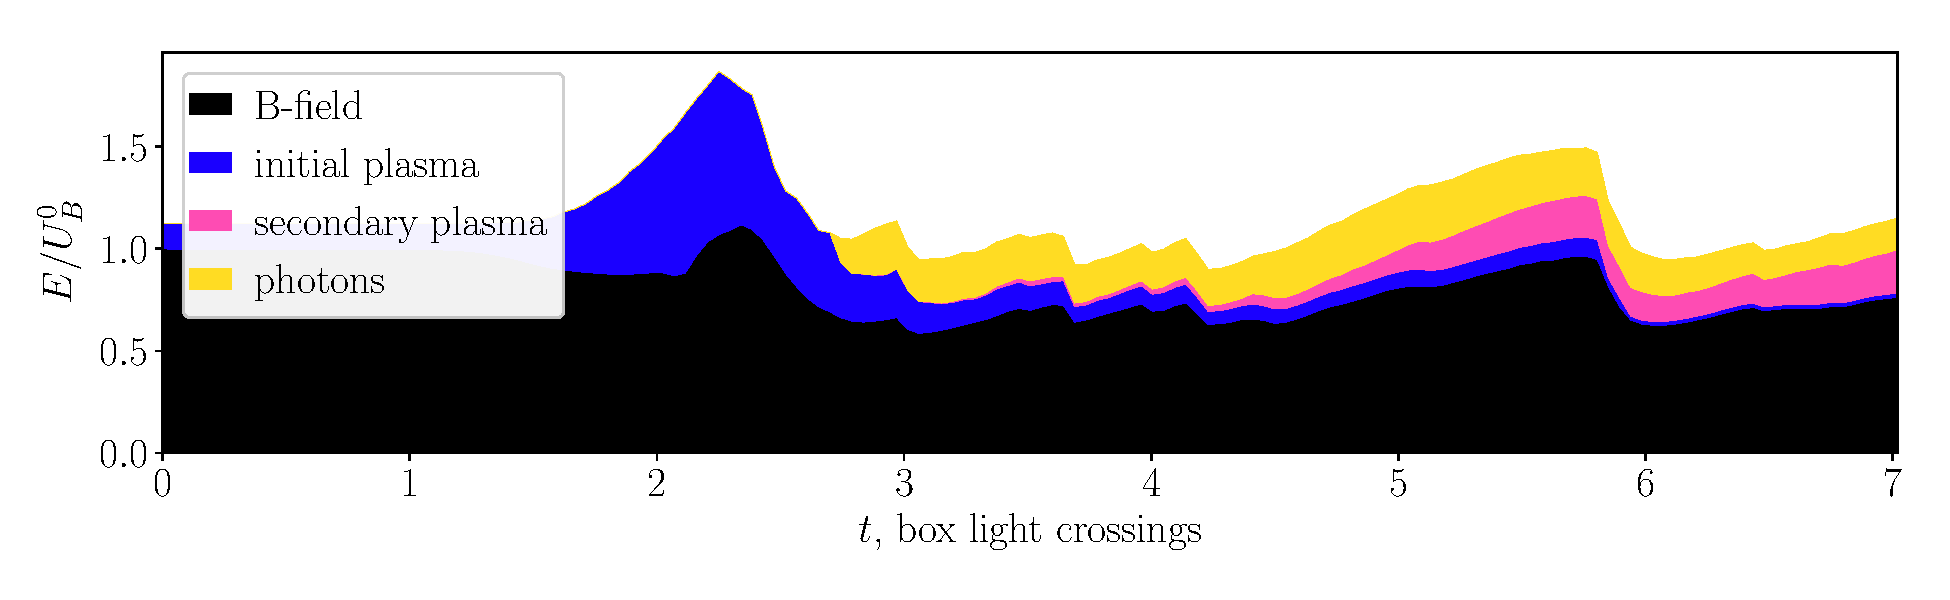
\includegraphics[width=0.9\textwidth]{figures/ch4-pairproduction/fig_b3.pdf}
    \caption{Energy partition in the simulation with $\sigma_{\rm c}=5000$, $\gamma_c=50$, $\gamma_{\rm rad}=1000$, $p_0=10^{-5}$. The energy is normalized by the initial magnetic field energy. Cooling and pair production is turned on at around three light-crossing times of the box. Large ``waves" are due to plasmoids forming, evolving and leaving the box in a few light-crossing times. One should keep in mind that the total energy of the magnetic field depends on the size of the region around the current sheet, and in this context it is rather artificial.}
    \label{fig:pairprod-energy_vs_time}
\end{figure}

%\end{appendices}

\singlespacing


% \clearpage
\bibliography{references}
\addcontentsline{toc}{chapter}{References}
\bibliographystyle{apalike2}

%\newpage

% If you do want an image in the colophon:
\begin{figure}
  \vspace{50pt}
  \centering
    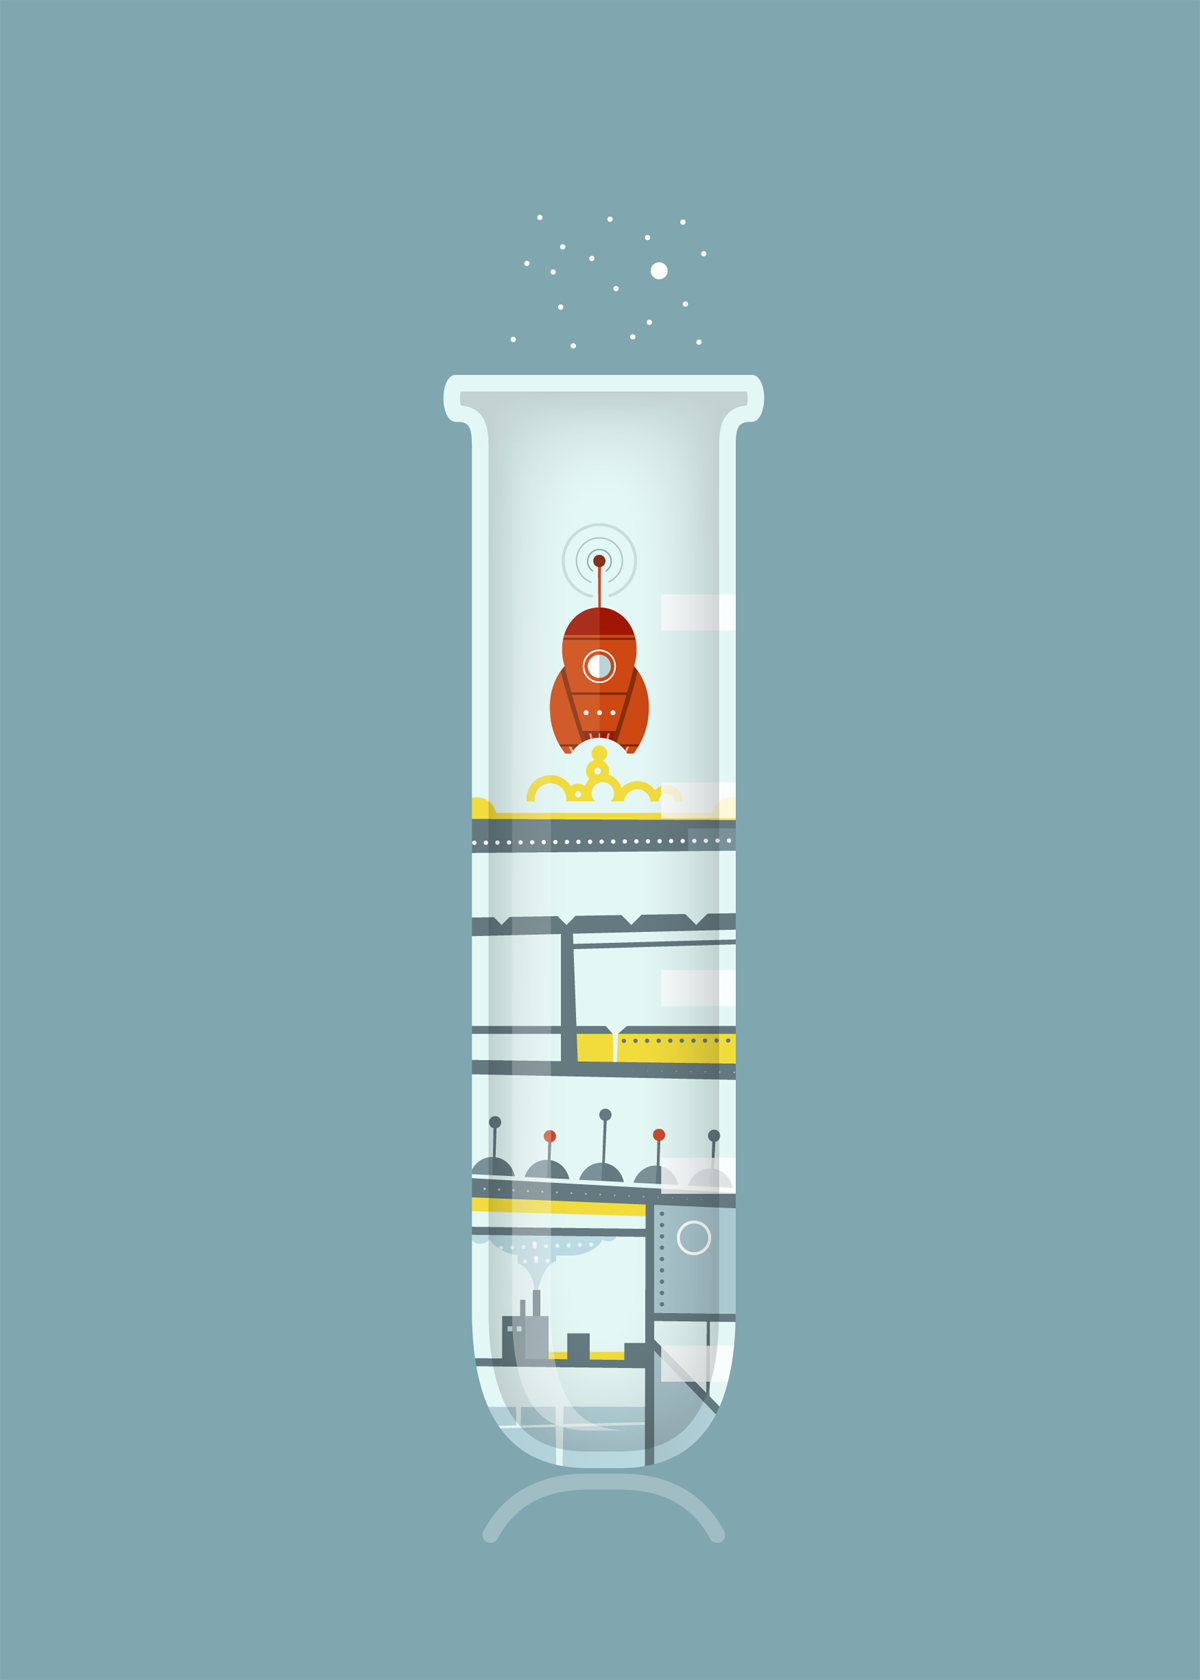
\includegraphics[width=0.51\textwidth]{endmatter/colophon.png}
\end{figure}

% If you don't want an image in the colophon:
% \vspace*{200pt}

\begin{center}
\parbox{200pt}{\lettrine[lines=3,slope=-2pt,nindent=-4pt]{\textcolor{SchoolColor}{T}}{his thesis was typeset} using \LaTeX, originally developed by Leslie Lamport and based on Donald Knuth's \TeX. The body text is set in 11 point Egenolff-Berner Garamond, a revival of Claude Garamont's humanist typeface. The above illustration, ``Science Experiment 02'', was created by Ben Schlitter and released under \href{http://creativecommons.org/licenses/by-nc-nd/3.0/}{\textsc{cc by-nc-nd 3.0}}. A template that can be used to format a PhD thesis with this look and feel has been released under the permissive \textsc{mit} (\textsc{x}11) license, and can be found online at \href{https://github.com/suchow/Dissertate}{github.com/suchow/Dissertate} or from its author, Jordan Suchow, at \href{mailto:suchow@post.harvard.edu}{suchow@post.harvard.edu}.}
\end{center}

\end{document}
